\documentclass[a4paper]{report}
\usepackage{amsmath}
\usepackage{amsfonts}
\usepackage{bm}
\usepackage{MnSymbol}
\usepackage{graphicx}
\usepackage{wrapfig}
\usepackage{enumitem}
\usepackage{comment}
\usepackage{import}
\usepackage{hyperref}
\usepackage{pgfplots}
\pgfplotsset{compat=1.18}
\title{MVE045 - Matematisk Analys}
\author{Max "Krysset" Hagman}
\begin{document}
\newcommand{\prim}[1]{#1^{\prime}}

\maketitle
\tableofcontents

%\chapter*{Introduktion}
\section*{föreläsningar}
Tre föreläsningar per vecka. På plats och ingen inspelning.\\
\\
Boken är Calculus av Adams. Upplaga 9 och 8 funkar också utav boken.
Kommer hålla sig 90-95\% av boken.\\
\\
Inga föreläsningsanteckningar.
Endast ifall inte allt material hinner täckas under föreläsningen.

\section*{Räkneövningar}
Två räkneövningar per vecka.\\
Det förväntas att man är aktiv på räkneövningar, annars är man inte välkommen.
Man ska inte sitta och vänta på lösningen och förväntas försöka lösa den.

\section*{Tenta}
Den 26 okt kl14:00 (antagligen), 8 uppgifter max 50p.
En av tentants frågor kommer vara att man ska bevisa en sats som har gåtts igenom under föreläsningarna.
Kursen har varit för lätt och dåligt formad.
Så tentan kommer inte vara typad.
Finns tentor från en systerkurs på data som man kommer kunna träna på.

\section*{Dugga}
Det kommer tre frivilliga duggor under kursen.
Klarar man alla frågorna på duggan får man ett extra poäng.
Man kan göra om duggorna flera gånger och får såklart använda boken.
Man får INTE sammarbeta på duggan eller hjälpa varandra.
Blir man tagen kan man skickas till disciplinnämnden.
Allt fusk kommer skickas till disciplinnämnden.

Kommer mer info om duggorna sen.\\

%Lessons
\chapter{Mängder och delmängder}
Mängder och delmängder är ett fundamentallt område inom matematik, alltså är det väldigt viktigt att kunna detta!

En mängd är en samling väldefinierade objekt.
Dessa objekt brukar kallas för \underline{element}.

En mängd $A$ bestående av elementen $a_1$, $a_2$, ... , $a_n$ skrivs som $A=[a_1,a_2, ... ,a_3]$
Om $A$ och $B$ är två olika mängder så betecknar $A\cup B$ alla element som tillhör $A$ eller $B$.
$A\cap B$ alla element som tillhör $A$ \underline{och} $B$.
Konstruktionen $A\cup B$ kallas för \underline{unionen} av $A$ och $B$ och $A\cap B$ kallas för \underline{snittet}.

Ett vanligt sätt att visualisera mängder är att genom så kallade \underline{venndiagram}:\\
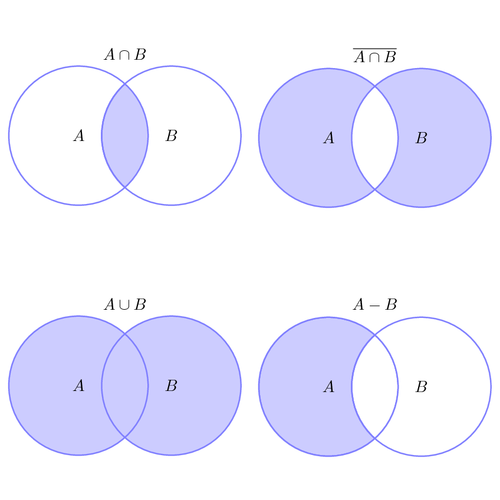
\includegraphics[scale=0.5]{lessons/lesson01/imgs/img01.png}
Ett par saker till
\begin{itemize}
    \item $\emptyset=\{\}$, den tomma mängden
    \item $A^c$ alla element som inte finns i $A$ (kallas \underline{komplementet})
\end{itemize}

\paragraph{Talmängder:} Mängder vars element är tal\\

Några viktiga talmängder som är grundläggande i matetmatik är:
\begin{itemize}
    \item $\mathbb{N}=\{0,1,2,3,...\}$ de \underline{naturliga talen}
    \item $\mathbb{Z}=\{...,-2-,-1,0,1,2,...\}$ \underline{heltalen}
    \item $\mathbb{Q}=\{\text{Alla talen på formen }\frac{p}{q}\}$, där $p,q\in\mathbb{Z},q\neq 0$
    \item $\mathbb{R}=\{\text{Alla decimaltal}\}$ de \underline{reella talen}
    \item $\mathbb{C}=\{\text{alla tal }a+ib\}$, de \underline{komplexa talen}
\end{itemize}

Inom matematisk analys är mängderna $\mathbb{R}$ och $\mathbb{C}$ speciellt i fokus.

\chapter{Intervall}
\paragraph{}
Ett \underline{intervall} är en delmängd av $\mathbb{R}$ som innehåller
minst två tal och \underline{alla} tal mellan två av sina element.\\
Mer konkret:\\
Öppet intervall
%\begin{wrapfigure}{l}{0.4\textwidth}
%bilder på respektive intervall
%infoga bild 2-4
, dvs $\{x\in\mathbb{R}:a<x<b\}$ skrivs $(a,b)$\\
, dvs $\{x\in\mathbb{R}:a\leq x\leq b\}$ skrivs $[a,]$\\
, dvs $\{x\in\mathbb{R}:a\leq x\leq b\}$ skrivs $[a,)$\\
%\end{wrapfigure}

\paragraph{Ex:}
Lös olikheten $\frac{x}{2}\geq 1+ \frac{4}{x}$ och uttryck svaret som ett intervall eller en union av flera intervall.
\paragraph{Lösning:}
Måste försöka skriva om olikheten till faktoriserad form!
\begin{equation*}
    \frac{x}{2}\geq 1+\frac{4}{x}\Leftrightarrow
    \frac{4+x}{x}\Leftrightarrow
    \frac{x}{2}-\frac{4+x}{x}\geq 0\Leftrightarrow
    \frac{x^2-2x-8}{2x}\geq 0
\end{equation*}
Hitta nollställena till $x^2-2x-8$ genom kvadratkomplettering!
\begin{equation*}
    x^2-2x-8=0 \Leftrightarrow
    x^2-2\cdot 1\cdot x+1-1-8=0 \Leftrightarrow
    (x-1)^2-9=0\Leftrightarrow
    x=1\pm \sqrt{9}=1\pm 3\Leftrightarrow
    x=4\text{ eller } x=-2
\end{equation*}
Kan nu skriva om $\frac{x^2-2x-8}{2x}\geq 0$ som $\frac{(x-4)(x+2)}{2x}\geq 0$.
Härifrån kan man använda metoden med teckenstudium:
$\begin{matrix}
                     &   & -2 &   & 0 &   & 4 &   \\
        \frac{1}{2}x & - & -  & - & | & + & + & + \\
        x-4          & - & -  & - & - & - & - & + \\
        x+2          & 0 & +  & + & + & + & + & + \\
        \text{Tot}   & - & 0  & + & | & - & 0 & +
    \end{matrix}$
Ser att $\frac{x^2-2x-8}{2x}\geq 0$ uppfylls i intervallen $[-2,0]$ och $[4,\infty)$ och kan skriva lösningen som $[-2,0)\cup[4,\infty)$.
\paragraph{\underline{Absolutbelopp}}
Absolutbelopp av ett tal $x\in\mathbb{R}$ definieras som:
\begin{equation*}
    %ska vara l-bracket
    |x|=\begin{matrix}
        x \text{, om } x\geq 0 \\
        -x \text{, om } x\leq 0
    \end{matrix}
\end{equation*}
Följande tolkning gäller:
Givet ett tal $a\in\mathbb{R}$ så gäller för alla $x\in\mathbb{R}$ att $|x-a|=$ avståndet mellan $x$ och $a$.
Vidare gäller också, givet ett fixt tal $D\geq 0$, att
$|x-a|\begin{matrix}< \\=\\>\end{matrix}D\Leftrightarrow$
mängden av alla $x\in\mathbb{R}$ vars avst. till $a$ är $\begin{matrix}<\\=\\>\end{matrix}D$,
dvs $|x-a|\begin{matrix}
        < \\=\\>
    \end{matrix}D\Leftrightarrow\begin{matrix}
        a-D<x<a+D \\
        x=a-D     \\
        x<a-D,x>a+D
    \end{matrix}$
\paragraph{Ex:} (P1.41)\\
Lös olikheten $|x+1| >|x-3|$ genom att tolka avs som ett avst. på talaxeln.
\paragraph{Lösning}
$|x+1| = |x-(-1)|=$ "avst mellan $x$ och $(-1)$"\\
$|x-3|=$ "avst. mellan $x$ och $3$"\\
Så "avst. mellan $x$ och $(-1)$" $ > $ "avst. mellan $x$ och $3$"
%infoga bild 5
Till höger om $1$ så kommer $x$ \underline{alltid} att vara längre från $(-1)$ än $3$.

\chapter{Komplexa tal}
Ett komplext tal $z\in\mathbb{C}$ kan alltid skrivas på formen $z=a+i\cdot b$ där\\
\begin{itemize}
    \item $a$ kallas för \underline{realdelen} av $z$ $Re(z)$
    \item $b$ kallas för \underline{imaginärdelen }av $z$ $Im(z)$
\end{itemize}

Den imaginära enheten $i$ löser definitionsmässigt ekv. $x^2+1=0$, dvs $i=\sqrt{-1}$
Rent visuellt kan man betrakta ett komplext tal $a + ib$ som en punkt i det komplexa talplanet.
%infoga bild 6
Det gäller att $r^2= |a+ib|^2= \vdots =a^2+b^2$.
Givet $r$ och argumentet $\theta$ kan \underline{alla} kompexa tal skrivas $z=r(cos(\theta)+i\cdot sin(\theta))$

\chapter{Funktioner}
\section{Funktioner och funktionsgrafer}
En funktion beskriver sambandet mellan in- och ut-data och kan bidra till ökad förståelse av hur olika processer hänger ihop.
%nästa mening är inte essentiell för kursen, kan antagligen raderas
Klassisk machine learning handlar mycket om att just hitta bra funktioner för att relatera in- och ut-data (supervised learning).

I envariabelanalys studeras funktioner som relaterar ett tal till ett annat.
Kan tänkas som en "regel" $f$ som \underline{avbildar} ett givet tal $x$ till ett annat tal $y$.

Alla de värdena som är tillåtna att mata in i $f$ kallas för funktionens \underline{definitionsmängd} och betecknas $D(f)$.
Mängden av alla $y$-värden som funktionen kan leverera kallas för \underline{värdemängden} och skrivs $R(f)$ (range).

\paragraph{Ex} Funktionen $f(x)=\frac{1}{x^2-1}$ har $D(f)=(-\infty,-1)\cup(-1,1)\cup(1,\infty)$.

\paragraph{} En funktionsgraf (eller bara en graf) givet en funktion $f$ utgörs av alla punkter $(x,y)=(x,f(x))$.
Några viktiga concept:
\begin{itemize}
    \item En funktion sägs vara \underline{jämn} om $f(-x)=f(x)$ då $(x\in D(f))$.\\
          Betyder att $f$ är symmetrisk m.a.p. y-axeln.
    \item En funktion sägs vara \underline{udda} om $f(-x)=-f(x)$.\\
          Betyder att $f$ är \underline{antispegelsymmetrisk} m.a.p. y-axeln.
    \item En funktion är \underline{injektiv} om det för varje par $x_1,x_2\in D(f)$ gäller att om $f(x_1)=f(x_2)$ så är $x_1=x_2$.
    \item En funktion $f$ som avbildar en mängd tal $\bm{x}$ på en annan mängd $\bm{y}$, dvs $f:\bm{x}\rightarrow\bm{y}$ sägs vara \underline{surjektiv} om $\bm{y}=R(f)$.
\end{itemize}

\section{Kompositioner}
En vanlig konstruktion är att kombinera två separata funktioner till en ny genom \underline{komposition}.
Kan göras på två sätt:
\begin{enumerate}
    \item $f\circ g(x):=f(g(x))$
    \item $g\circ f(x):=g(f(x))$
\end{enumerate}
Notera att $f\circ g\neq g\circ f$ i allmänhet!

\chapter{Polynom och rationella funktioner}
Ett polynom är en funktion som kan skrivas som:
$P(x)=a_1\cdot x^n+a_{n-1}\cdot x^{n-1}+...+ax+a_0$ där $a_n,... ,a_0\in\mathbb{R}$ kallas för polynomets \underline{koefficienter} och talet $n$ (positivt heltal) kallas för polynomets \underline{grad}.
En rationell funktion $R(x)$ är en funktion som kan skrivas som en kvot på två polynom $P(x)$ och $Q(x)$, dvs $R(x)=\frac{P(x)}{Q(x)}$.
Definitionsmängden $D(R)$ begränsas enbart av nollställena till $Q(x)$, dvs. $D(R)=\mathbb{R}\setminus \{x\in\mathbb{R}:Q(x)=0\}$.

\section{Polynomdivision}
Rationella tal kan alltid skrivas som en heltalsdel + rest:\\
$\frac{29}{6}=\frac{4*6+5}{6}=\frac{4*6}{6}+\frac{5}{6}=4+\frac{5}{6}$\\
Motsv. funkar även för rationella funktioner  och metoden för att hita "heltalsdelen" och "resten" kalla \underline{polynomdivison}.

\paragraph{Ex (P6.18)} Uttryck $\frac{x^4+x^2}{x^3+x^2+1}$ som summan av ett polynom och en rationell funktion.
\subparagraph{Lösning}~\\
\begin{wrapfigure}{l}{0.4\textwidth}
    \vspace{-15pt}
    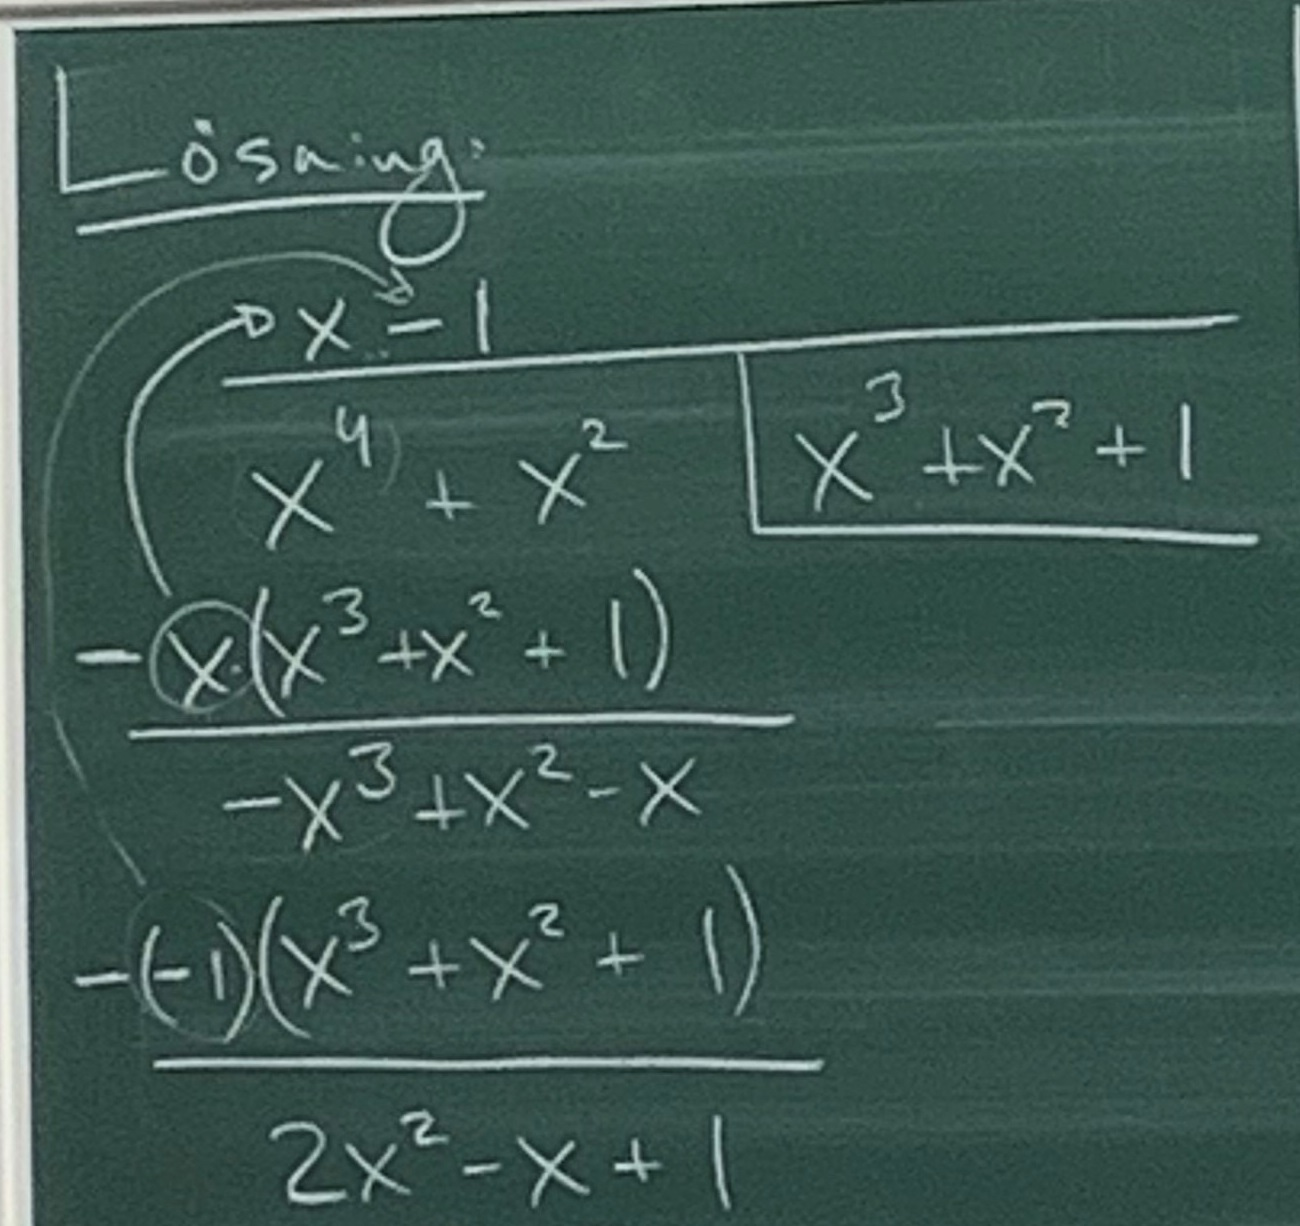
\includegraphics[scale=0.1]{lessons/lesson02/imgs/img01.jpg}\\
\end{wrapfigure}
Eftersom polynomet $2x^2-x+1$ har lägre grad än nämnaren $x^3+x^2+1$ tar divisionsalgo. slut.
Vi har fått att $\frac{x^4+x^2}{x^3+x^2+1}=(x-1)+\frac{2x^2-x+1}{x^3+x^2+1}\Box$.
\clearpage
\paragraph{} Enligt \underline{Aritmetikens fundamentalsats} så kan \underline{alla} positiva heltal alltid skrivas som en unik faktorisering av \underline{primtal}, t.ex $120=2^3\cdot 3\cdot 5$.
Liknande resultat finns för polynom! Algebrans fundementsats säger att varje polynom av grad $n$ har exakt $n$ st. nollställen (ev. komplexa och räknade med multiplicitet).
Vidare gäller också \underline{faktorsatsen}:
\paragraph{Sats} Talet $r$ är en \underline{rot} (dvs ett nollställe) till ett polynom $P$ av grad minst $1$ \underline{om och endast om} $(x-r)$ är en faktor av $P(x)$.
\\\\
Eftersom alla polynom $P$ av grad $\geq 1$ har precis $n$ st. nollställen säg $r_1,...,r_n$ kan man \underline{alltid} faktorisera ett polynom som $P(x)=(x-r_1)\cdot(x-r_2)\cdot ... \cdot(x-r_n)$.

\chapter{Grundläggande trigonometri}
De trigonometriska frunktionererna $\cos\theta$ och $\sin\theta$ def. som $x$- respektive y-koordinaten på den punkt på \underline{enhetscirkeln} som motsvaras av vinkeln $\theta$.
\begin{figure}[h!]
    \centering
    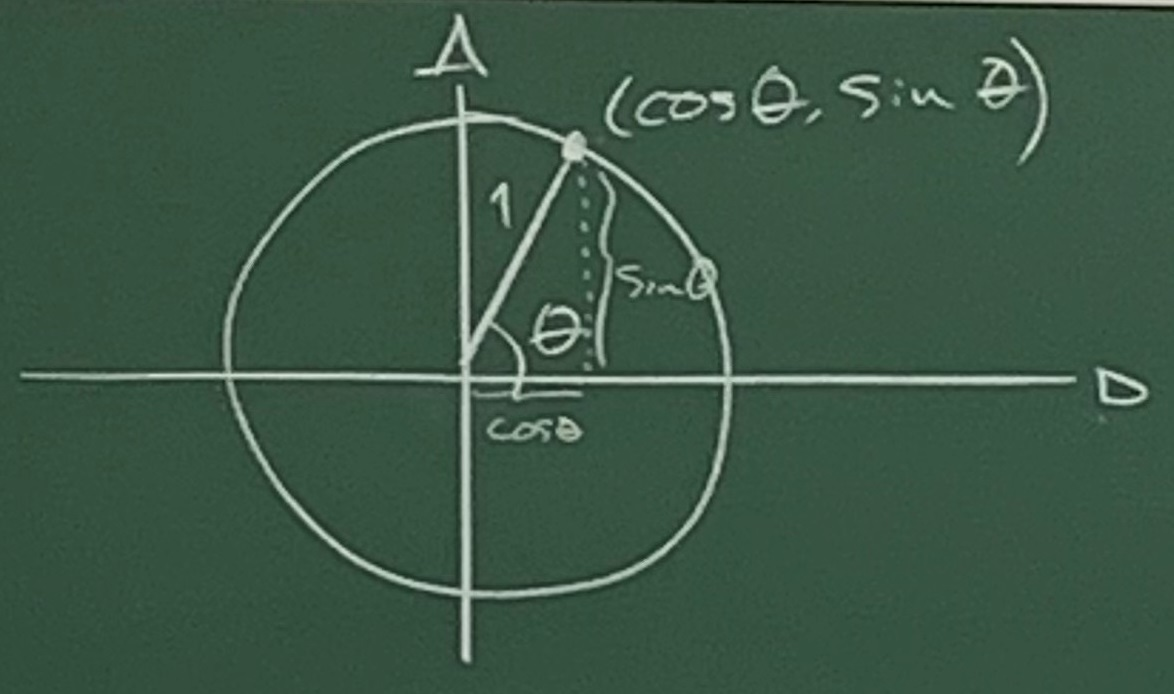
\includegraphics[scale=0.2]{lessons/lesson02/imgs/img02.jpg}
\end{figure}
Pythagoras sats ger omedelbart att $\cos^2\theta+\sin\theta=1$, även kallat trigonometriska ettan.
Vinkeln $\theta$ mäts oftast i radianer men kan också mätas i geader.
Det gäller att $\pi$ radianer motsvarar $180^\circ$ grader.

\paragraph{}Utifrån $\sin$ och $\cos$ definieras vidare funktionen tangens som $tan\theta:=\frac{\sin\theta}{\cos\theta}$.
Två trigonometriska samband som är viktiga är sinus- och cosinus-satsen:
%infoga bild 3
\begin{figure}[h!]
    \centering
    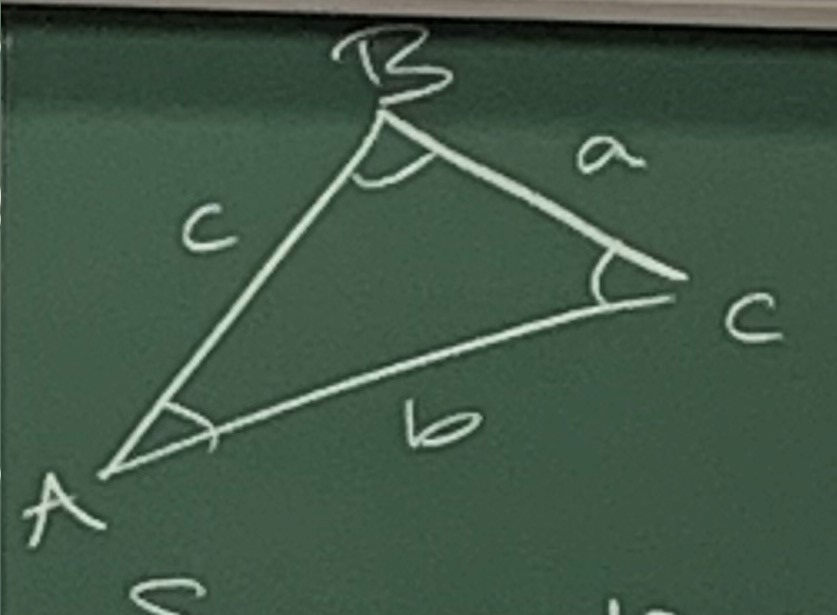
\includegraphics[scale=0.1]{lessons/lesson02/imgs/img03.jpg}
\end{figure}
\subparagraph{Sinussatsen} $\frac{\sin A}{a}=\frac{\sin B}{b}=\frac{\sin C}{c}$
\subparagraph{Cosinussatsen} $a^2=b^2+c^2-2b\cos A$

\paragraph{Ex (P6.53)} Visa att arean på en godtycklig triangel $ABC$ kan beräknas som $\frac{1}{2}bc\cdot\sin A=\frac{1}{2}ab\cdot\sin C=\frac{1}{2}ac\cdot\sin B$.
\subparagraph{Lösning}
Area$=\frac{x_z\cdot y}{2}+\frac{x_2\cdot y}{2}=\frac{x_1\cdot y + x_2\cdot y}{2}$.
Men $\sin A=\frac{y}{c}\Rightarrow y=c\cdot\sin A \Rightarrow Area=\frac{x_1\cdot c\sin A+x_2c\sin A}{2}=\frac{(x_1+x_2)\cdot c\cdot\sin A}{2}=\{x_1+x_2=b\}=\frac{1}{2}bc\sin A$.
De andra formulerna följer analogt. $\Box$
\begin{figure}[h!]
    \centering
    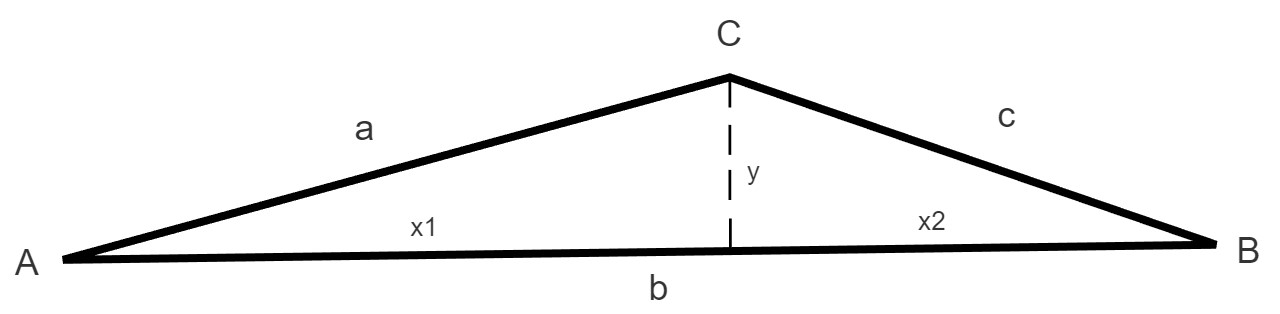
\includegraphics[scale=0.2]{lessons/lesson02/imgs/img04.jpg}
\end{figure}
\chapter{Talföljder och gränsvärden}
Studium av talföljder är ett av matematikens mest klassiska områden.
Vi har exempelvis:
\begin{itemize}
    \item Fibonacci-talföljden, $0,1,1,2,3,5,8,...$, återfinns i olika sammanhang i naturen.
    \item Primtalssekvensen, $2,3,5,7,11,13,17,...$, finns formel för att beskriva sekvensen? (olöst)
\end{itemize}
Ska försöka formalisera begreppen i synnerhet för oändligt långa talföljder.\\
Låt $\{a_1,a_2,a_3,...\}=\{a_n\}, n\in\mathbb{N}$ vara en godtycklig talföljd.
Man säger att $\{a_n\}$ är:
\begin{itemize}
    \item Begränsad ovan-/underifrån om det finns ett tal $L$ sådant att $a_n\leq L$/$a_n\geq L$ $\forall n=1,2,3,...$.
    \item Begränsad om den är begränsad \underline{både} ovan- och underifrån.
    \item Positiv/Negativ om $a_n\geq 0$/$a_n\leq 0, \forall n=1,2,...$
    \item Växande/Avtagande om $a_{n+1}\geq a_n$/$a_{n+1}\leq a_n,\forall n=1,2,3,...$
    \item Monoton om talföljden är antingen växande eller avtagande
    \item Alternerande om $a_{n+1}\cdot a_n <0,\forall n=1,2,3,...$
\end{itemize}
Ett viktigt begrepp för talföljder (och funktioner) är \underline{konvergens}, dvs. om talföljden "stannar av" och håller sig oförändrad om man bara kollar tillräckligt långt in i följden (dvs. n stort).
%infoga bild 1
Måste försöka precisera vad detta betyder ren matematiskt.
\paragraph{Definition} Konvergent talföld\\
Man säger att en talföljd ${a_n}$ konvergerar mot $L\in\mathbb{R}$ och skriver $\lim_{n \to \infty}a_n=L$, om det för varhe positivt tal $\varepsilon > 0 $ existerar ett positivt heltal $N$ så att det för alla $n\leq N$ gäller att $|a_n-L|\leq\varepsilon$.
\subparagraph{Intuitivt} $\{a_n\}$ konvergerar mot $L$ om \underline{alla} tal tillräckligt långt in i följden ligger godtyckligt nära talet $L$.
Av detta följder "enkelt" att:
\begin{itemize}
    \item om $\{a_n\}$ konvergerar så är den begränsad.
    \item om $\{a_n\}$ är begränsad ovanifrån och växande så är $\{a_n\}$ konvergent.
          Motsvarande för begränsad underifrån och avtagande.
\end{itemize}
Bra räknelagar:
\begin{itemize}
    \item $\lim_{n \to \infty}(\frac{a_n}{b_n})=\frac{\lim_{n \to \infty}a_n}{\lim_{n \to \infty}b_n}$, om $\lim_{n \to \infty}b_n\neq 0$
    \item om $a_n\leq b_n\leq c_n$ och $\lim_{n \to \infty}a_n=\lim_{n \to \infty}c_n=L\Rightarrow \lim_{n \to \infty}b_n=L$.
\end{itemize}

\paragraph{Ex (9.1.25)} Bestäm om möjligt det tal $L$ som $a_n=\sqrt{n^2+n}-\sqrt{n^2-1}$ konvergerar mot då $n\to\infty$
\subparagraph{Lösning} Det gäller att
\begin{equation*}
    \sqrt{n^2-n}-\sqrt{n^2-1}=\sqrt{(n+1)\cdot n}-\sqrt{(n+1)(n-1)}=\sqrt{n+1}\cdot(\sqrt{n}-\sqrt{n-1})=
\end{equation*}
\begin{equation*}
    \sqrt{n+1}\cdot\frac{(\sqrt{n}\sqrt{n-1})\cdot(\sqrt{n}+\sqrt{n-1})}{\sqrt{n}+\sqrt{n-1}}=\sqrt{n+1}\cdot\frac{(n-(n-1))}{\sqrt{n}+\sqrt{n-1}}=\frac{\sqrt{n+1}}{\sqrt{n}+\sqrt{n-1}}
\end{equation*}
\begin{equation*}
    \text{och } \frac{\sqrt{n+1}}{\sqrt{n}+\sqrt{n-1}}\leq\frac{\sqrt{n}}{\sqrt{n}+\sqrt{n}}=\frac{1}{2}
\end{equation*}
\begin{equation*}
    \frac{\sqrt{n+1}}{\sqrt{n}+\sqrt{n+1}}\leq\frac{\sqrt{n+1}}{\sqrt{n-1}+\sqrt{n-1}}\cdot\frac{\sqrt{n-1}}{\sqrt{n-1}}=\frac{\sqrt{n^2-1}}{2(n-1)}\leq\frac{\sqrt{n^2}}{2(n-1)}=
\end{equation*}
\begin{equation*}
    \frac{n}{2(n-1)}=\frac{1}{2(1-\frac{1}{n})}\overrightarrow{n\to\infty}\frac{1}{2}
\end{equation*}
så $\lim_{n\to\infty}\sqrt{n^2+n}-\sqrt{n^2-1}=\frac{1}{2}\Box$
\\
\paragraph{} Ett av de mest kraftfulla verktygen inom matematisk analys är \underline{gränsvärden} för funktioner, dvs $\lim_{x \to a}f(x),a\in\mathbb{R}$.
Det ger oss derivator, integraler, differentialekvationer, ...
Hur ska man definiera gränsvärdet $\lim_{x \to a}f(x)$?
Skulle kunna inspireras av definitionen för talföljder.
\paragraph{Definition (försök)} Man säger att $f(x)$ konvergerar mot värdet $L\in\mathbb{R}$ då $x$ går mot $a\in\mathbb{R}$ om det för varje talföljd $\{x_n\}$ s.a $\lim_{n\to\infty}x_n=a$ gäller att $\lim_{n\to\infty}f(x)=L$.
\\\\Bättre definition i liknande riktning är dock.
\paragraph{Definition} Man säger att $f(x)$ går mot gränsvärdet
$L\in\mathbb{R}$ då $x$ går mot $a\in\mathbb{R}$ och skriver
$\lim_{x\to a}f(x)=L$, om det för varje tal $\varepsilon > 0$
existerar ett annat tal $\delta > 0$ (som ev. beror av $\varepsilon$) s.a.
om $0< |x-a| <\delta$ så ligger $x$ i $f$s definitionsmängd och
$|f(x)-L|<varepsilon$.

\paragraph{Ex}
\begin{enumerate}
    \item $f\to L_1$, när $x\to a_1$?
          %infoga bild 2
          Ja! Går alltid att hitta $\delta>0$ s.a. $|f(x)-L_1|<\varepsilon$ oavsett $\varepsilon$.
    \item $f\to L_2$, när $x\to a_1$?
          %infoga bild 3
          Omöjligt att hitta $\delta>0$ s.a. $|f(x)-L_2|<\varepsilon$ om $\varepsilon$ litet.
\end{enumerate}

\paragraph{Ex (1.5.19)}Använd definitionen av gränsvärde för att bevisa att
\begin{equation*}
    \lim_{x\to 1}\sqrt{x}=1
\end{equation*}
\subparagraph{Lösning} Vill hitta $\delta > 0$ så att
$|\sqrt{x}-1|<\varepsilon$ så länge som $0< |x-1| <\delta$
(givet vilket $\varepsilon>0$ som helst).
Gäller att $|\sqrt{x}-1<\varepsilon\Leftrightarrow-\varepsilon<\sqrt{x}-1<\varepsilon\Rightarrow 1-\varepsilon<\sqrt{x}<1+\varepsilon$.
$\left\{\begin{matrix}
        \text{Om }0<\varepsilon<\sqrt{x}\leq 1: 1-\varepsilon<\sqrt{x}<1+\varepsilon\Rightarrow(1-\varepsilon)^2<x<(1+\varepsilon)^2 \\
        \text{Om }\varepsilon>1:1-\varepsilon<\sqrt{x}<1+\varepsilon\Rightarrow 0<x<(1+\varepsilon)^2
    \end{matrix}\right.$
Notera att $(1-\varepsilon)^2<x<(1+\varepsilon)^2$ \underline{alltid} implicerar att $1-\varepsilon<\sqrt{x}<1+\varepsilon$ dvs $|\sqrt{x}-1|<\varepsilon$.
\begin{equation*}
    (1-\varepsilon)^2<x<(1-\varepsilon)^2\Leftrightarrow 1-2\varepsilon+\varepsilon^3<x<1+2\varepsilon+\varepsilon^2\Leftrightarrow-\varepsilon(2-\varepsilon)<x-1<\varepsilon\cdot(2+\varepsilon)
\end{equation*}
%infoga bild 4
så \begin{equation*}
    -\varepsilon\cdot(2-\varepsilon)<x-1<\varepsilon\cdot(2-\varepsilon)\Rightarrow-\varepsilon(2-\varepsilon)<x-1<\varepsilon(2+\varepsilon)
\end{equation*}
om $\varepsilon<2$.
Välj därför $\delta=\varepsilon\cdot(2-\varepsilon)$ om $\varepsilon<2$.
För $\varepsilon\leq 2$, välj t.ex $\delta=1$ eftersom $|x-1|<1\Rightarrow-1<\sqrt{x}-1<0\Rightarrow-2<\sqrt{x}-1<2\Rightarrow|\sqrt{x}-1|<2\leq\varepsilon\Box$

\section{Kontinuitet}
Matematisk analys handlar om studier av funktioner (och ekvationer) definierade på $\mathbb{R}$ eller $\mathbb{C}$.\\
Frågeställningar och intuition för ämnet hämtas ofta från fysik/teknik där funktioner bär på någon form av information.\\
Vår definition av funktion är att det är "en regel" som avbildar ett tal $x$ i en given definitionsmängd $D(f)$ till ett annat tal $y$ i en värdemängd.
Gruppen av sådana regler är \underline{enorm}, dvs. det finns ett ouppräkneligt antal möjliga funktioner, och de flesta av dom skulle inte vara användabara för modellering av verkliga system.

\paragraph{Ex}
$f(x) = \begin{matrix}
        1\text{, om }x\in\mathbb{Q} \\
        0\text{, om }x\notin\mathbb{Q}
    \end{matrix}$ (Dirichlet-funktionen)\\
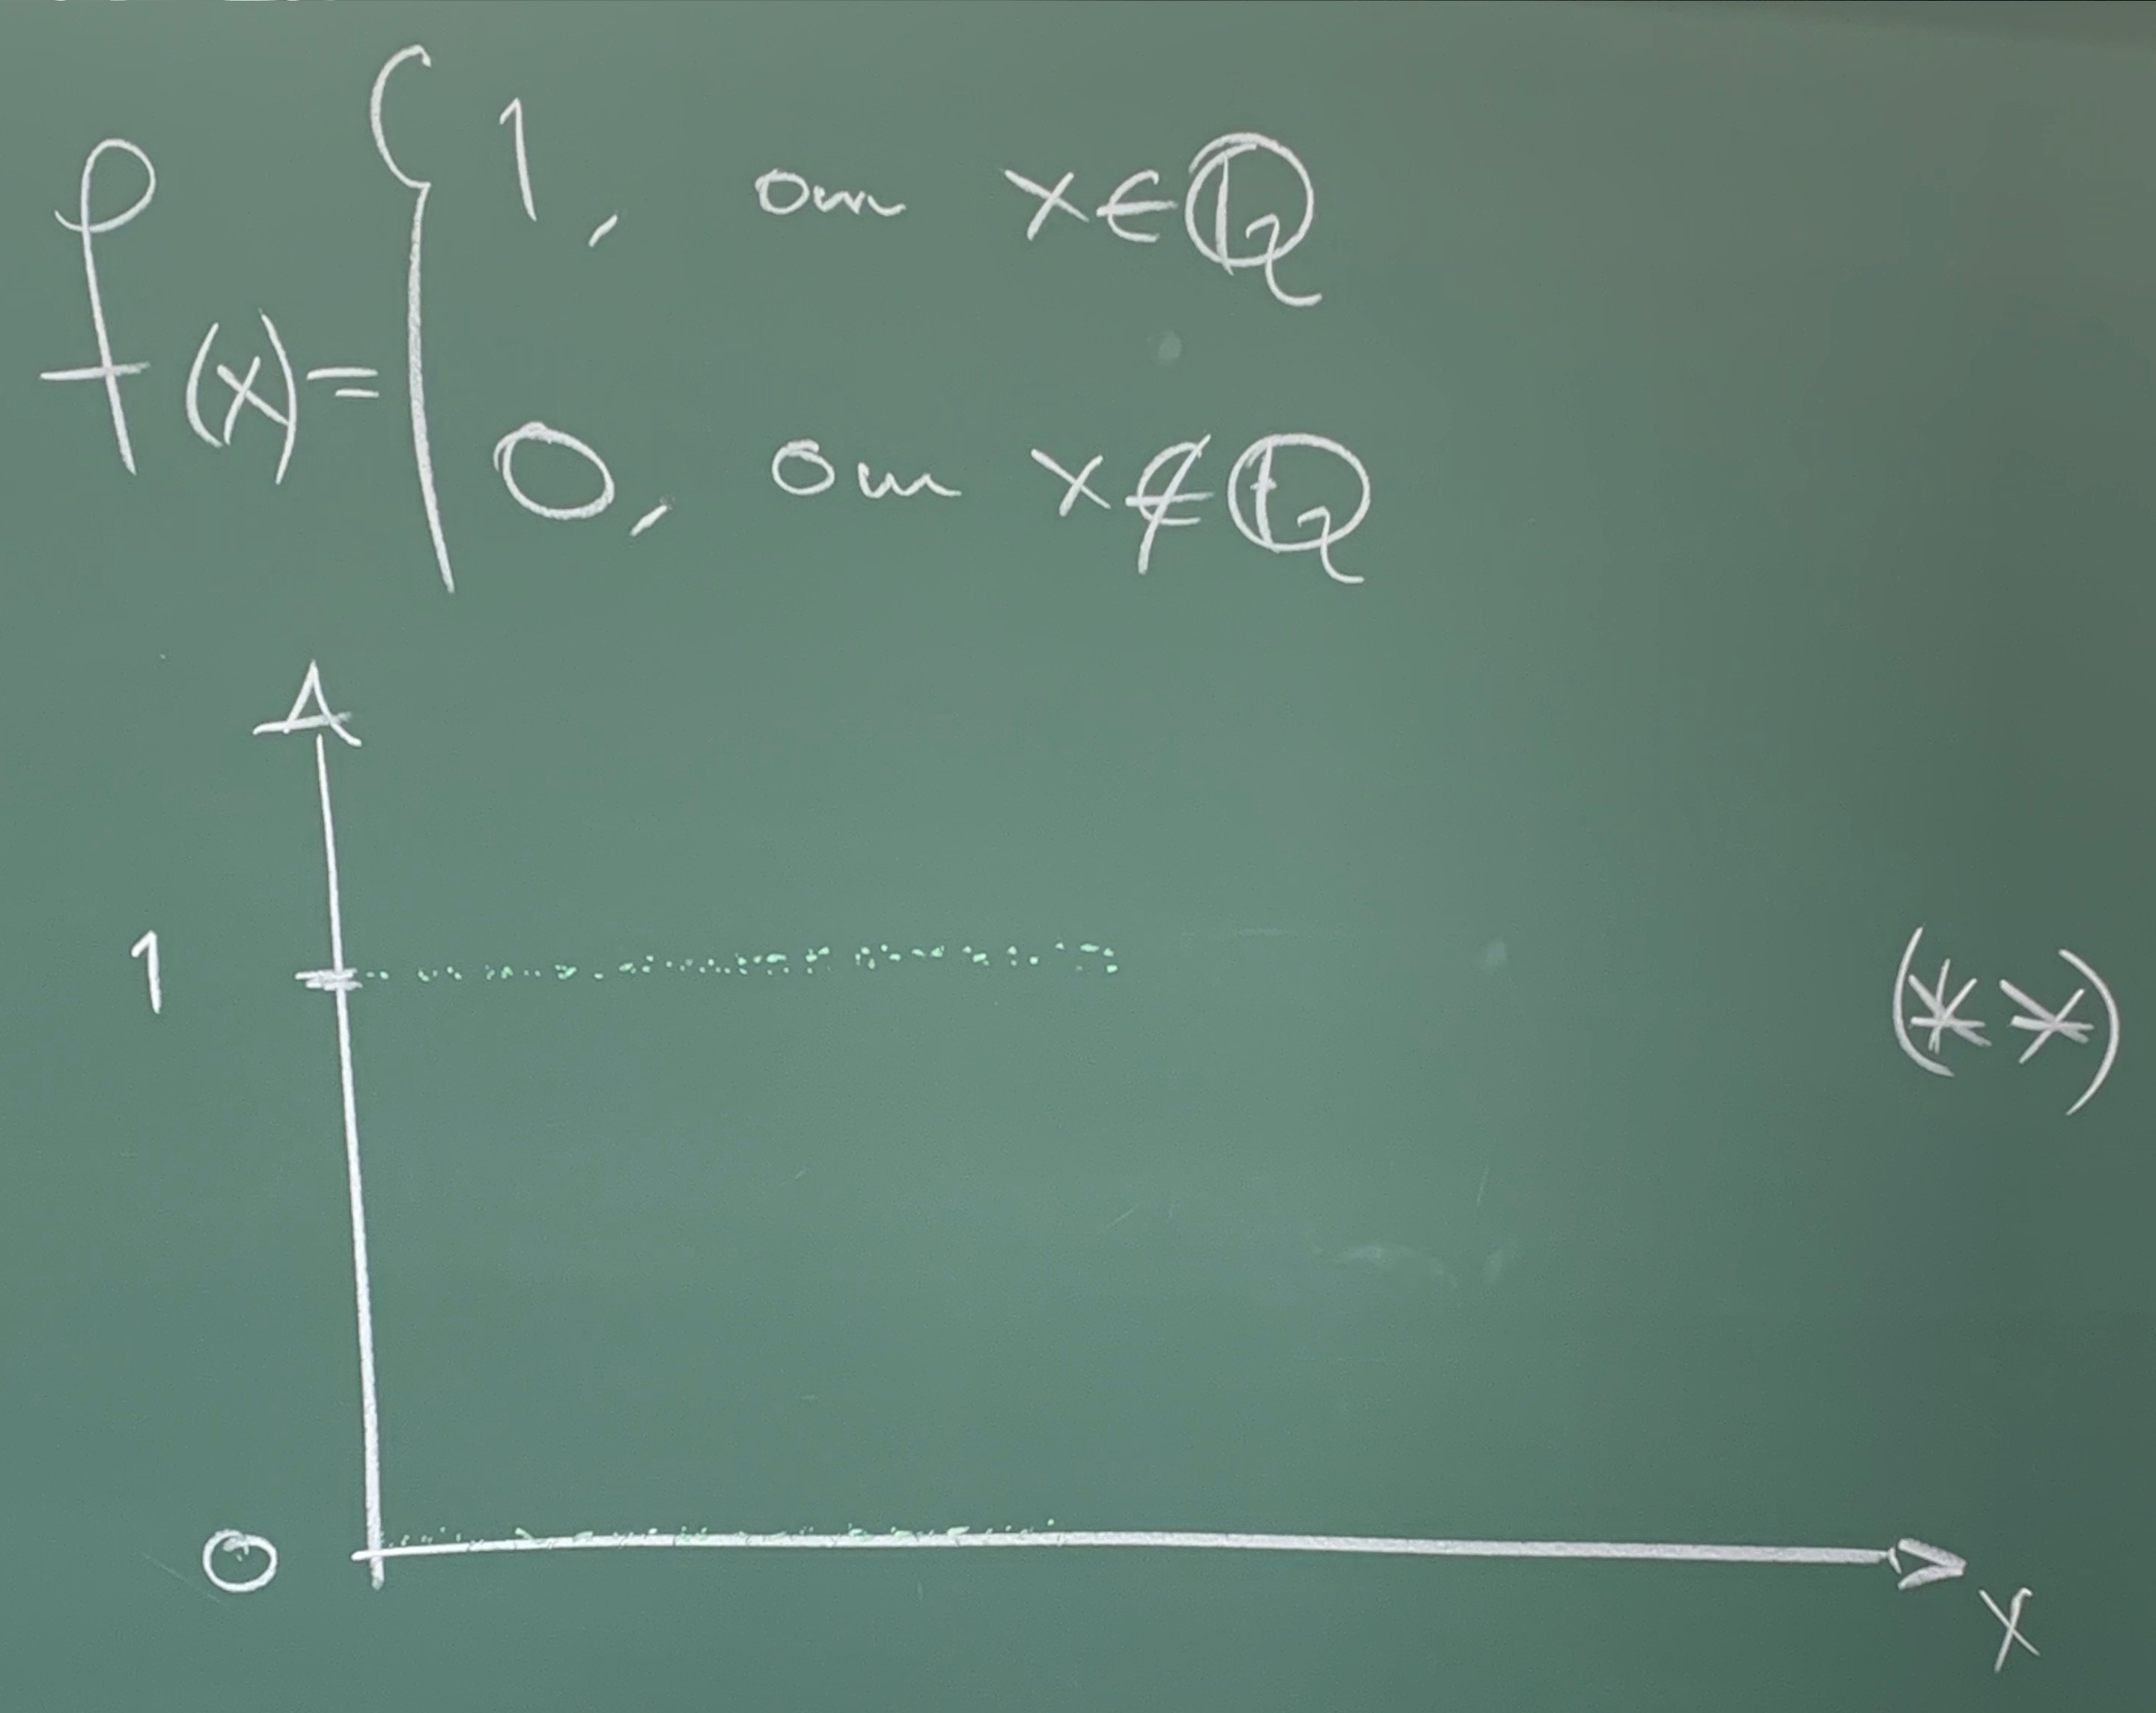
\includegraphics[scale=0.1]{lessons/lesson04/imgs/img01.jpg}

Om man drar en funktion slumpmässigt från mängden av alla funktioner så skulle man nästan säkert dra något i stil med dirichlet funktionen.
Måste därför hitta vettig begränsad klass av funktioner för att kunna hitta meningsfulla matematiska resultat.
En sådan klass är de \underline{kontinuerliga} funktionerna.

\paragraph{Definition} (Kontinuerlig funktion)
Man säger att en funktion $f$ är \underline{kontinuerlig} i punkten $x=c$ (som antas vara en mindre punkt i $D(f)$) om $\lim_{x\to c}f(x)=f(c)$.
Om antingen $\lim_{x\to c}f(x)$ inte existerar \underline{eller} existerar men inte är lika med $f(c)$ säger man att $f$ är \underline{diskontinuerlig} i $x=c$.
Vad betyder detta? Jo, det betyder att "funktionen hänger ihop" i $x=c$.\\
\includegraphics[scale=0.1]{lessons/lesson04/imgs/img02.jpg}\\
Man säger att en funktion $f$ är kontinuerlig på ett helt intervall $I$ om $f$ är kontinuerlig i varje punkt $x\in I$.\\
Hur hanterar man ändpunkterna i $I$? Till exempel om $I=[a,b]$, vad ska gäla för $x\to a$ och $x=b$?
Jo, $f$ ska vara \underline{högerkontinuerlig} i $x=a$ och \underline{vänsterkontinuerlig} i $x=b$.
\begin{itemize}
    \item Man säger att en funktion $f$ är vänsterkontinuerlig i en punkt $x=c$ om $\lim_{x\to c^-}f(x)=f(c)$.
    \item Man säger att en funktion $f$ är högerkontinuerlig i en punkt $x=c$ om $\lim_{x\to c^+}f(x)=f(c)$.
\end{itemize}
Så, $f$ benämns som kontinuerlig i \underline{randpunkter} till ett intervall (till exempel $a$ och $b$ för $[a,b]$) om den är höger- respektive vänsterkontinuerlig.\\
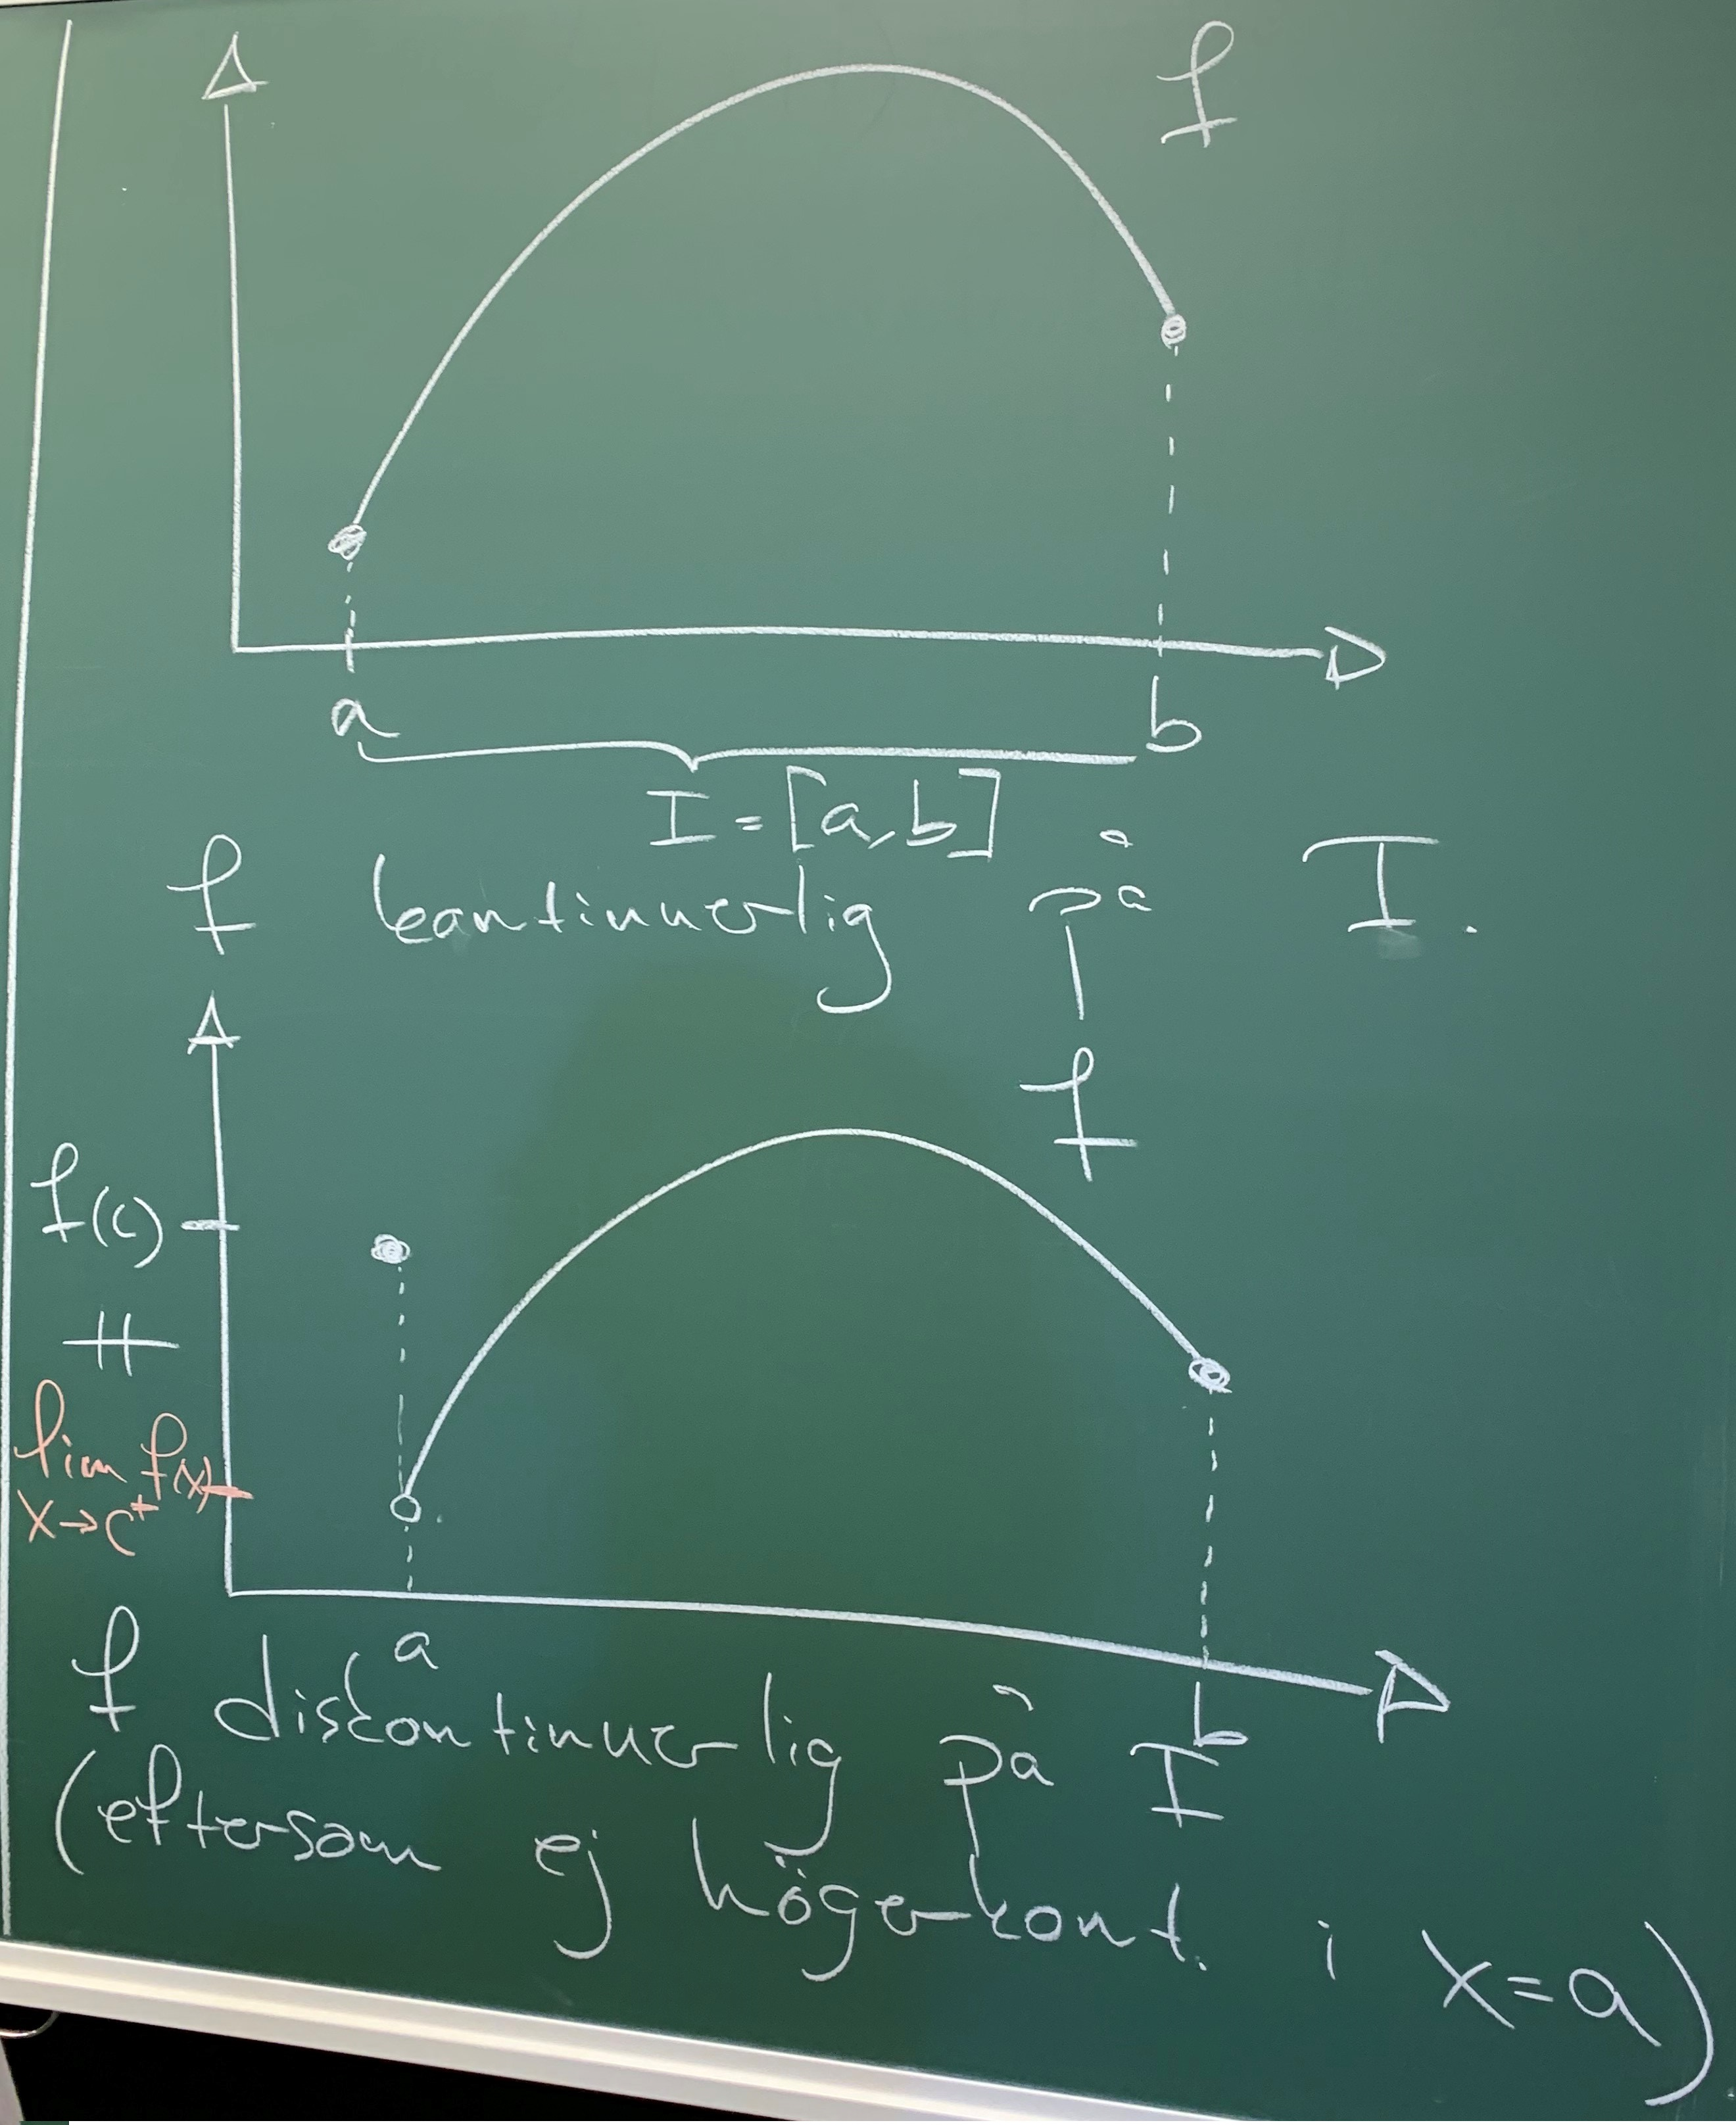
\includegraphics[scale=0.1]{lessons/lesson04/imgs/img03.jpg}\\

\paragraph{Ex (1.4.9)} Beskriv var i sin definitionsmängd som följande funktion är kontinuerlig, vänster- respektive högerkontinuerlig och diskontinuerlig.
\begin{equation*}
    f(x)=\begin{matrix}
        \frac{1}{x^2}\text{, om }x\neq 0 \\
        0\text{, om }x=0
    \end{matrix}
\end{equation*}
\subparagraph*{Lösning}
Försök att skissa funktionen.
\begin{itemize}
    \item funktionen $\frac{1}{x^2}$ är alltid positiv
    \item Om $x$ är \underline{stort} (antingen positivt eller negativt) så är $\frac{1}{x^2}\approx 0^+$
    \item Om $x$ är nära $0$ (antingen positivt eller negativt) så är $\frac{1}{x^2}\approx+\infty$
    \item Uppenbart tt $\frac{1}{x^2}$ är växande på $(-\infty,0)$ och avtagande på $(0,\infty)$.
\end{itemize}
%infoga bild 4
%\includegraphics[scale=0.1]{lessons/lesson04/imgs/img04.jpg}\\
Alltså, $f$ är kontinuerlig för alla $x\in\mathbb{R}\setminus \{0\}$ eftersom $\lim_{x\to a}\frac{1}{x^2}=\frac{1}{a^2}=f(x)$ för alla $a\in\mathbb{R}\setminus\{0\}$.
I $x=0$ är $f$ diskontinuerlig eftersom $\lim_{x\to 0}f(x)=\lim_{x\to 0}\frac{1}{x^2}=+\infty$ och $f(0)=0$ och $0\neq\infty\Box$

\paragraph{Ex (1.4.16)} Hur ska man definiera funktionen $f(x)=\frac{x^2-2}{x^4-4}$ i punkten $x=\sqrt{2}$ för att den ska bli kontinuerlig där?
\subparagraph{Lösning} Vad händer i $x=\sqrt{2}$?\\
\begin{equation*}
    f(\sqrt{2})=\frac{\sqrt{2}^2-2}{\sqrt{2}^4-4}=\frac{2-2}{4-4}=\frac{0}{0}\text{???}
\end{equation*}
Vill studera gränsvärdet $\lim_{x\to \sqrt{2}}f(x)$.
\begin{equation*}
    f(x)=\frac{\sqrt{2}^2-2}{\sqrt{2}^4-4}=\frac{x^2-2}{(x^2-2)(x^2+2)}=\frac{1}{x^2+2}\text{ }\overrightarrow{x\to\sqrt{2}}\text{ }\frac{1}{4}
\end{equation*}
Vi ser att $f$ kan naturligt definieras i punkten $x=\sqrt{2}$ även om det inte var uppenbart från början.
Genom att sätta $f(\sqrt{2})=\frac{1}{4}$ så blir funktionen kontinuerlig i $x=\sqrt{2}$, dvs.
$f(x)=
    \begin{matrix}
        \frac{x^2-2}{x^4-4}\text{, om } x\neq\sqrt{2} \\
        \frac{1}{4}\text{, om }x=\sqrt{2}
    \end{matrix}\Box$

\paragraph{Ex (1.5.3)} Beräkna gränsvärdet
\begin{equation*}
    \lim_{x\to 3}\frac{ |5-2x| - |x-2| }{ |x-5| - |3x-7| }
\end{equation*}
\subparagraph{Lösning} Måste reda ut hur det olika absolutbeloppen beter sig i en omgivning av $x=3$.
\begin{equation*}
    |5-2x|=
    \begin{matrix}
        5-2x\text{ om } 5-2x\geq 0 \Leftrightarrow x \leq \frac{5}{2}=2,5 \\
        -(5-2x)\text{ om } 5-2x < 0 \Leftrightarrow x > 2,5
    \end{matrix}
\end{equation*}
\begin{equation*}
    |x-2|=
    \begin{matrix}
        x-2\text{ om } x-2\geq 0 \Leftrightarrow x \geq 2 \\
        -(x-2)\text{ om } x-2 < 0 \Leftrightarrow x <2
    \end{matrix}
\end{equation*}
\begin{equation*}
    |x-5|=
    \begin{matrix}
        x-5\text{ om } x-5\geq 0 \Leftrightarrow x \geq 5 \\
        -(x-5)\text{ om } x-5 < 0 \Leftrightarrow x < 5
    \end{matrix}
\end{equation*}
\begin{equation*}
    |3x-7|=
    \begin{matrix}
        3x-7\text{ om } 3x-7 \geq 0 \Leftrightarrow x\geq \frac{7}{3}\approx 2,33 \\
        -(3x-7)\text{ om } 3x-7 < 0 \Leftrightarrow x < 2,33
    \end{matrix}
\end{equation*}
Vi kan alltså skriva gränsvärdet som:
\begin{equation*}
    \lim_{x\to 3}\frac{2x-5-x+2}{5-x-3x+7}=\lim_{x\to 3}\frac{x-3}{-4x+12}=\lim_{x\to 3}\frac{x-3}{-4(x-3)}=\frac{1}{4}\Box
\end{equation*}
Är alla kontinuerliga funktioner "välartade" och alltid lämpliga för att beskriva något slags verklighet?\\
Nej.
\begin{itemize}
    \item Finns massa verkliga situationer som kräver diskontinuerliga funktioner för att kunna beskrivas.
    \item finns väldigt "konstiga" kontinuerliga funktioner.
          %Infoga bild 1
\end{itemize}
Lite grundläggande egenskaper för kontinuerliga funktioner.\\
Om $f$ och $g$ är två kontinuerliga funktioner i $c\in\mathbb{R}$ så gäller att:\\
\begin{itemize}
    \item $f+g$, $f-g$ och $f\cdot g$ är kontinuerliga i $x=c$ och $\frac{f}{g}$, $\frac{g}{f}$ om $g(c)$ respektive $f(c)\neq 0$
    \item $k\cdot f$ är kontinuerlig i $x=c$ för alla konstanter $k\in\mathbb{R}$.
    \item $(f)^\frac{1}{n}$ är kontinuerlig i $x=c,n\in\mathbb{N}$ (givet att $f(c)\geq 0$ om $n$ är jämnt)
\end{itemize}
vad gäller om man vill kompononera ihop kontinuerliga funktioner?
\paragraph{Sats} (Komposition av kont. funktioner)\\
Om $f\circ g := f(g(x))$ är definierad på ett intervall som innehåller
$x=C$ och $f$ är kontinuerlig i $x=L$ och $\lim_{x\to c}g(x)=L$
så gäller att:
\begin{equation*}
    \lim_{x\to c}f(g(x))=f(L)=f(\lim_{x\to c}g(x))
\end{equation*}
Speciellt om $g$ är kontinuerlig i $x=c$ (dvs. $\lim_{x\to c}g(x)=g(c)$)
så är kompositionen $f\circ g$ också kontinuerlig i $x=c$.

\subparagraph{Bevis} Vill bevisa att om $f$ är kontinuerlig i $x=L$ och
$\lim_{x\to c}g(x)=L$ så är $\lim_{x\to c} f(g(x))=f(L)$ (Resten följer per automatik).\\
Använd definitionen av grändsvärde!\\
Vet att $f$ är kontinuerlig i $y=L$, dvs. $\lim_{y\to L}f(y)=f(L)$
vilket definitionsmässigt betyder att det för varje $\varepsilon > 0$
finns ett tal $\gamma > 0$ s.a. om $|y-L|<\gamma$ så är $|f(y)-f(L)|<\varepsilon$.\\
Vidare, eftersom $\lim_{x\to c}g(x)=L$ så finns det ett tal $\delta > 0$
sådant att om $|x-c|<\delta$ så är $|g(x)-L|<\gamma$ för vilket $\gamma>0$ som helst.
I vårt fall är vi intresserade av fallet där $y=g(x)$ och av tidigare
gäller således att om bara $0< |x-c| <\varepsilon$ så kommer
$|f(g(x))-f(L)|<\varepsilon$ oavsett hur vi väljer $\varepsilon>0$.\\
Men detta betyder att $\lim_{x\to c}f(g(x))=f(L)$ och vi har därmed visat att
$\lim_{x\to c}f(g(x))=f(L)=f(\lim_{x\to c}g(x))$ och speciellt att
$f\circ g$ är kontinuerlig i $x=c$ om $g$ är kontinuerlig i $x=c$. $\Box$

~\\
Vi förstätter med lite allmänna egenskaper för kontinuerliga funktioner.
\paragraph{Sats} (kontinuerliga funktioner är begränsade) (tenta)\\
Om $f$ är kontinuerlig på intervallet $[a,b]$ så är $f$ begränsad över samma intervall.\\\\
För att bevisa detta ska vi använda Bolzano-Weierstrass sats.
\paragraph{Sats} (Bolzano-Weierstrass) (tenta)\\
Låt $\{a_n\}$ vara en oändlig och begränsad talföljd.
Då finns en delföljd av $\{a_n\}$ som är konvergent!\\
Intuition: Givet att $\{a_n\}$ är begränsad så kan man alltid plocka
ihop en ny talföljd med element tagna i ordning från $\{a_n\}$,
säg $\{a_{n_k}\}$, så att denna följd konvergerar.

\paragraph{Bevis} (kontinuerliga funktioner är begränsade)\\
Använder ett så kallad "motsägelsebevis", dvs. antag att satsen inte stämmer och visar att detta leder till något orimligt eller omöjligt.\\
Antag att $f$ är kontinuerlig på $[a,b]$ men \underline{inte} begränsad ovanifrån på $[a,b]$.
I så fall gäller att det för varje heltal $k>0$ finns ett $x_k\in[a,b]$ så att $f(x_k)>k$ (eftersom $f$ växer obegränsat på $[a,b]$ enligt antagande).
Alltså kan vi konstruera en talföljd $\{x_n\}$ där \underline{alla} $x_n\in[a,b]$ och $f(x_n)>n$.
Men om alla $x_n\in[a,b]$ så måste talföljden $\{x_n\}$ vara begränsad (eftersom $a\leq x_ \leq b$).
Av Bolzano-Weierstrass stats finns därför en delföljd till $\{x_n\}$ säg $\{x_{n_k}\}$ som är konvergent.
Beteckna denna delföljds gränsvärde med $x$, dvs $\lim_{k\to \infty}x_{n_k}=x$.
Eftersom $x\in[a,b]$ och $f$ är kontinuerlig i $x$ (eftersom $f$ kontinuerlig på hela $[a,b]$ enligt förutsättning) så gäller per definition att $\lim_{h\to \infty}f(x_{n_k})=f(x)$.
Men eftersom $f(x_n)>n$ så måste $\lim_{k\to\infty}f(x_{n_k})=\infty$.
Detta motsäger att $f$ är kontinuerlig på $[a,b]$!\\
Slutsats: $f$ måste vara begränsad ovanifrån.\\
Liknande resonemang gäller för att visa att $f$ även är måste vara begränsad underifrån och därmed begränsad. $\Box$

\paragraph{Sats} (min-max-satsen)\\
Låt $f$ vara en kontinuerlig funktion på $[a,b]$ (där $|a|,|b|<\infty$).
Då existerar \underline{alltid} tal $p,q\in[a,b]$ sådana att för alla $x\in[a,b]$, $f(p)\leq f(x)\leq f(q)$ dvs. $f$ har ett minimum $m=f(p)$ och ett maximum $M=f(q)$.
%infoga bild 2

\paragraph{Sats} (satsen om mellanliggande värden)\\
Låt $f$ vara en kontinuerlig funktion på $[a,b]$ och låt $s$ vara ett tal mellan $f(a)$ och $f(b)$.
Då existerar det alltid ett tal $c\in[a,b]$ så att $f(c)=s$.

\chapter{Derivatan}
Ett av de mest fundamentala koncepten inom matematisk analys är \underline{derivata}.
Handlar om hur snabbt en given funktion förändras i närheten av en punkt $x$.
Kan hämta inspiration från medelhastigheter.\\
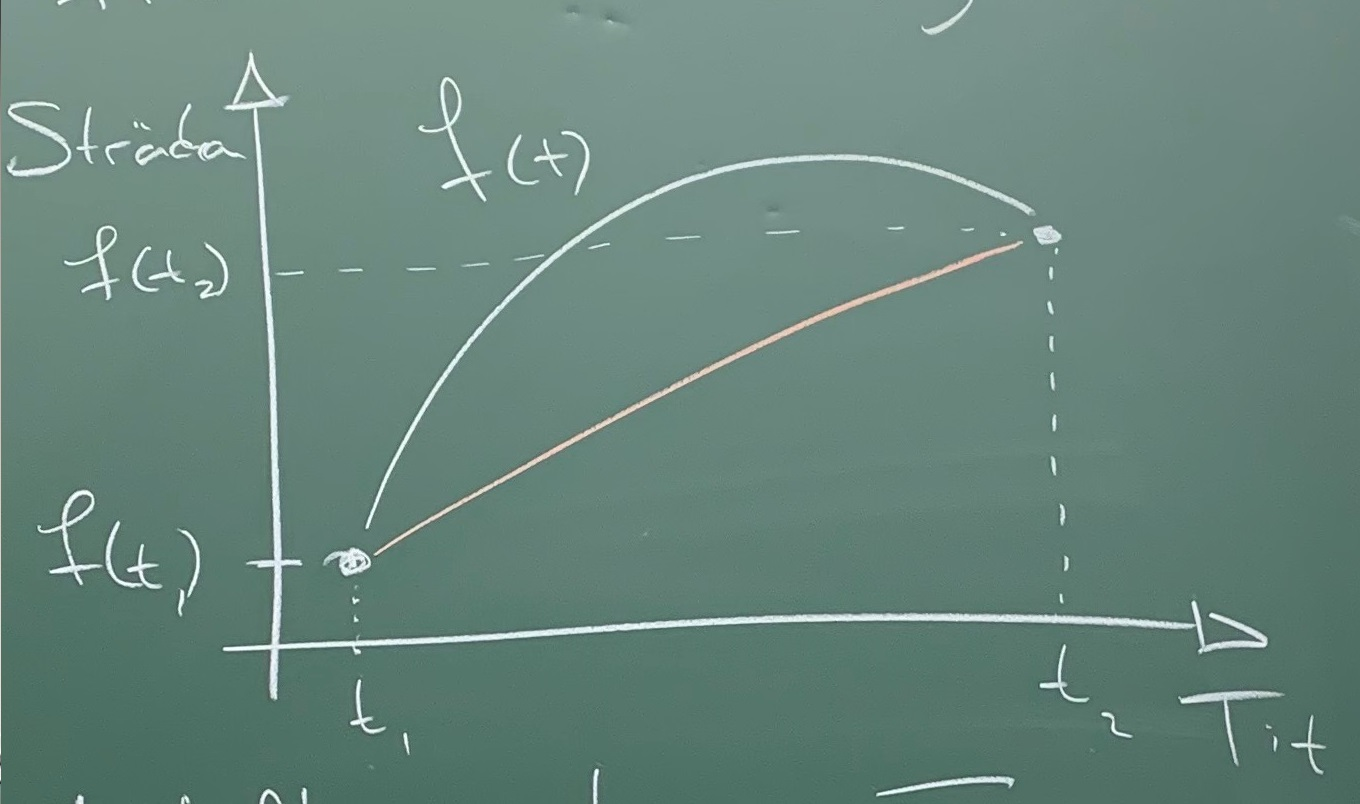
\includegraphics[scale=0.2]{lessons/lesson06/imgs/img01.jpg}\\
Medelhastigheten $\overline{v}$ mellan $t_1$ och $t_2$ är $\overline{v}=\frac{f(t_2)-f(t_1)}{t_2-t_1}$.
Just $\overline{v}$ är dessutom lutningen på den linje som går från $(t_1,f(t_1))$ till $t_2,f(t_2)$.
\begin{equation*}
    \overline{v}=\frac{y-f(t_1)}{x-t_1}\Leftrightarrow y=\overline{v}(x-t_1)+f(t_1)
\end{equation*}
Uppenbart att ju närmre $t_2$ är $t_1$ desto mer kan $\overline{v}$ tolkas som den momentana hastigheten i $t_1$
och "snittlinjen" övergår till att bli en tangent.\\
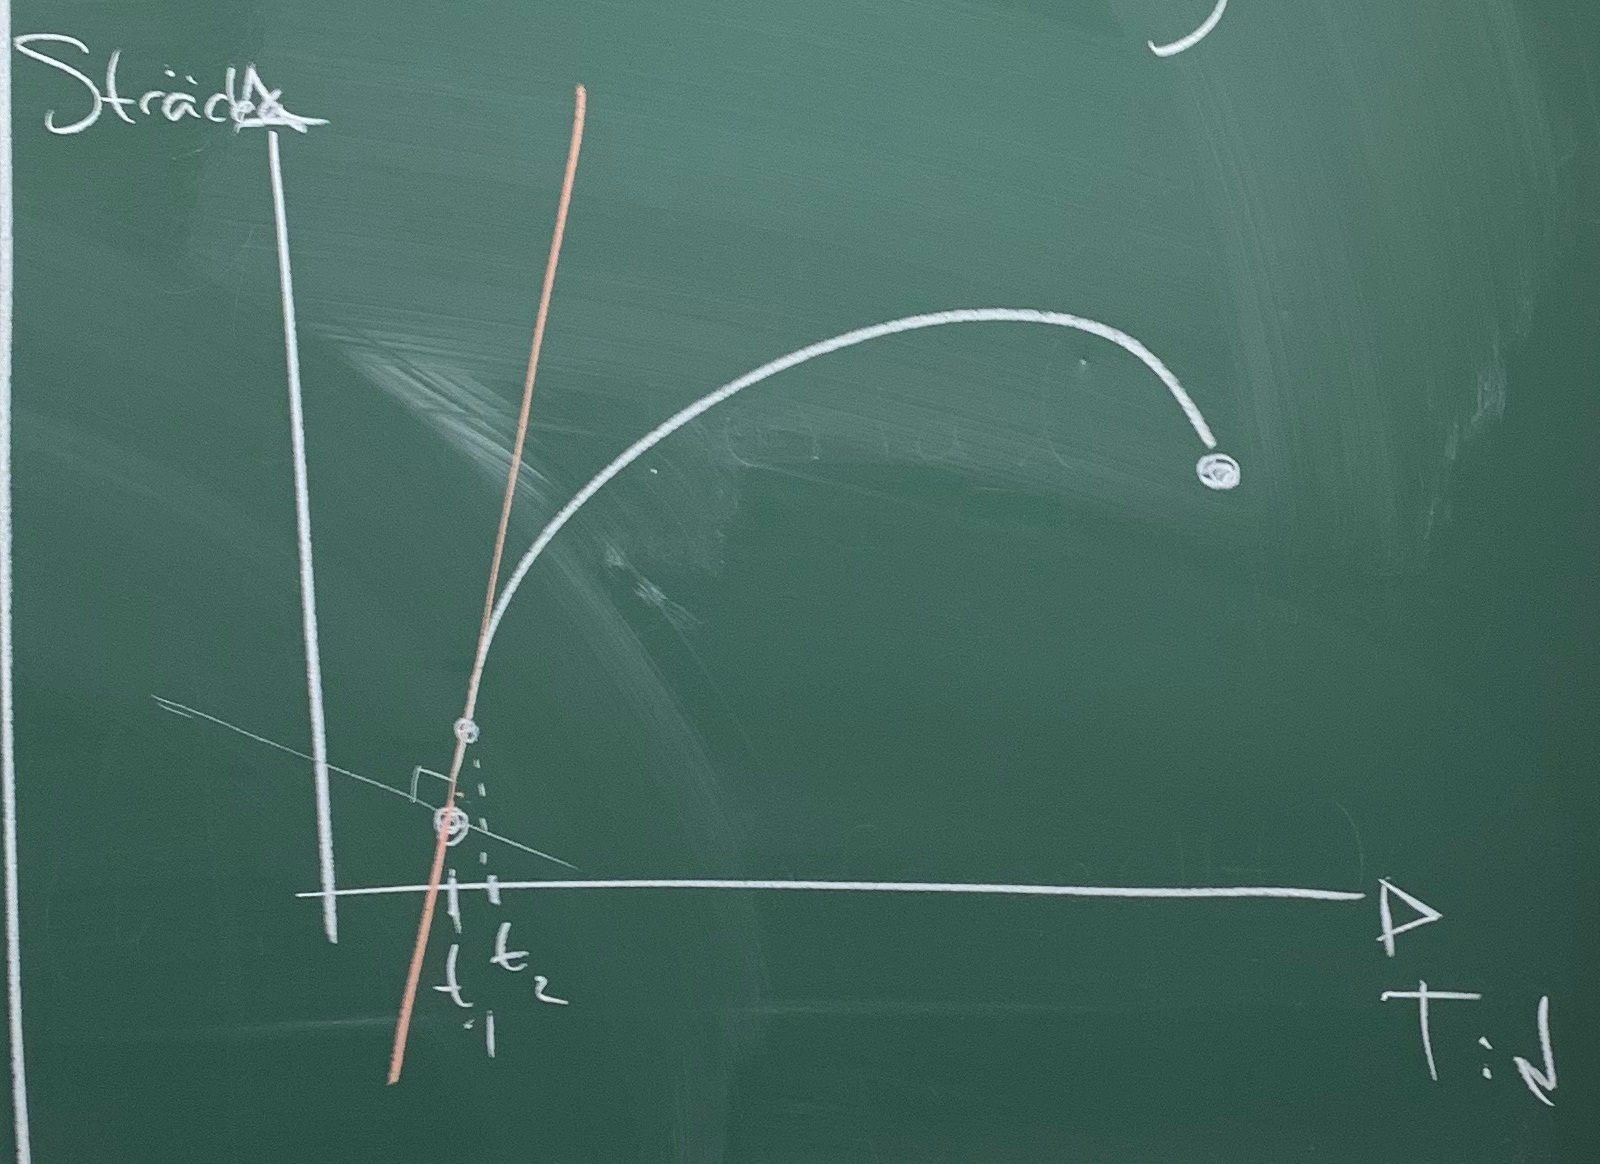
\includegraphics[scale=0.2]{lessons/lesson06/imgs/img02.jpg}\\
\\
Naturligt  att definiera den momentana hastigheten i en punkt $x_0$ för en given funktion $f$ som
\begin{equation*}
    \lim_{h\to 0}\frac{f(x_0+h)-f(x_0)}{(x_0+h)-x_0}=\lim_{h\to 0}\frac{f(x_0+h)-f(x_0)}{h}
\end{equation*}
Om detta gränsvärde existerar så kallas det för \underline{derivatan} av $f$ i $x=x_0$ och betecknas som $f^\prime(x_0)$.
Geometriskt så kan $f^\prime(x_0)$ tolkas som tangentlinjens lutning i $x=x_0$ för grafen till $f$.

Precis som för gränsvärden kan man definiera höger- och vänsterderivatan som:
\begin{equation*}
    f_+^\prime(x_0^+)=\lim_{h\to 0}\frac{f(x_0+h)-f(x_0)}{h}
\end{equation*}
\begin{equation*}
    f_-^\prime(x_0^-)=\lim_{h\to 0}\frac{f(x_0+h)-f(x_0)}{h}
\end{equation*}
En funktion $f$ sägs vara deriverbar på ett intervall $[a,b]$ om den är deriverbar i varje punkt $x\in[a,b]$
och höger- respektive vänsterderiverbar i $a$ respektive $b$.

från derivatan kan man enkelt beräkna lutningen för \underline{normalen}, dvs. den linjen som är vinkelrät mot tangenten som:
\begin{equation*}
    \text{Normalens lutning i }x_0=-\frac{1}{f^\prime(x_0)}
\end{equation*}
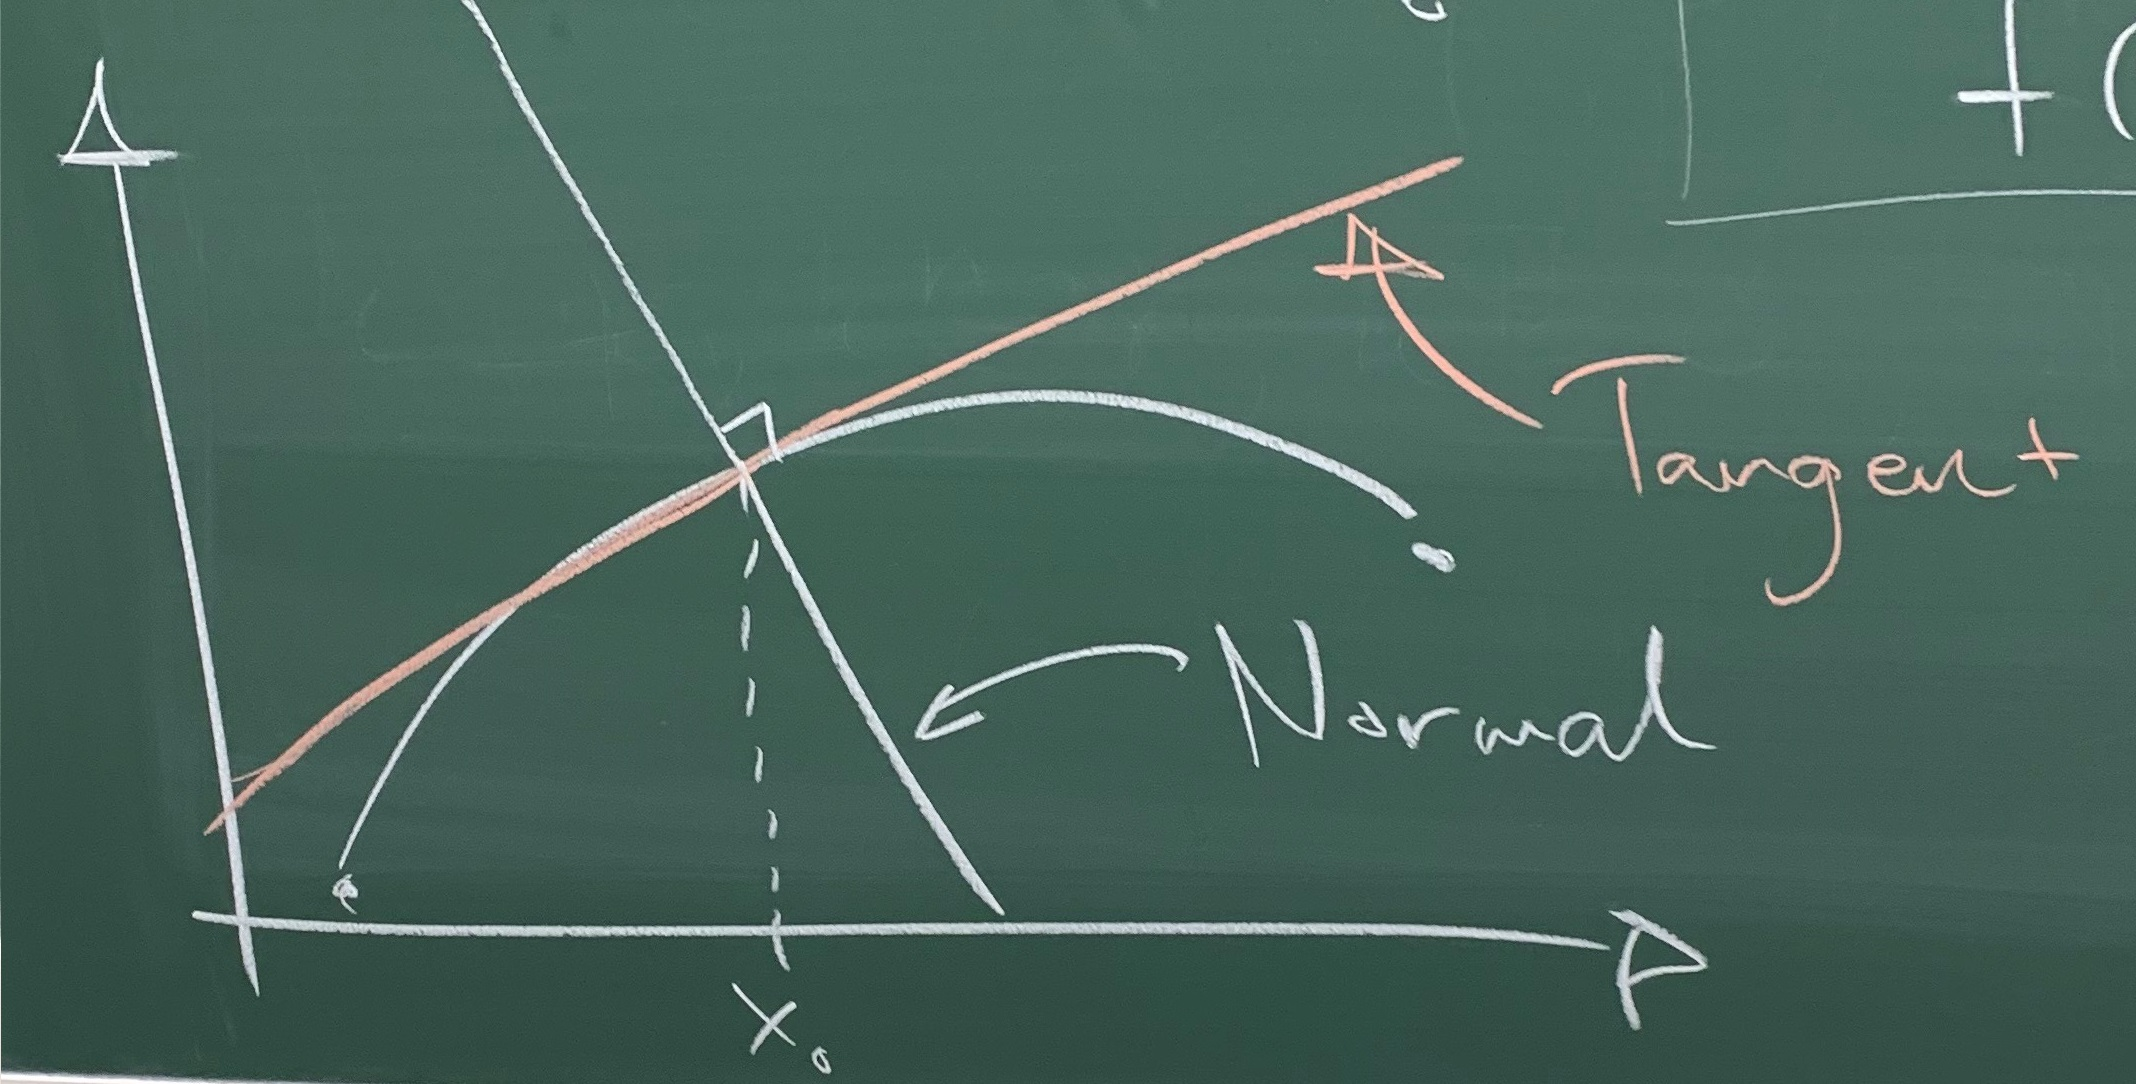
\includegraphics[scale=0.2]{lessons/lesson06/imgs/img03.jpg}

\paragraph{Ex}(2.2.21)\\
Använd derivatans definition och beräkna $f^\prime(x)$ givet funktionen $f(x)=\frac{1}{\sqrt{1+x^2}}$.
\subparagraph{Lösning}
Vi måste beräkna följande gränsvärde då $h\to 0$:
\begin{equation*}
    \frac{f(x+h)-f(h)}{h}=
    \frac{1}{\sqrt{1+(x+h)^2}}-\frac{1}{\sqrt{1+x^2}}=
    \frac{\frac{\sqrt{1+x^2}-\sqrt{1+(x+h)^2}}{\sqrt{1+(x+h)^2}\cdot\sqrt{1+x^2}}}{h}=
\end{equation*}
\begin{equation*}
    \frac{\sqrt{1+x^2}-\sqrt{1+(x+h)^2}}{h\sqrt{1+(x+h)^2}\sqrt{1+x^2}}\cdot\frac{\sqrt{1+x^2}+\sqrt{1+(x+h)^2}}{\sqrt{1+x^2}+\sqrt{1+(x+h)^2}}=
\end{equation*}
\begin{equation*}
    \frac{(1+x^2)-(1+(x+h)^2)}{h\sqrt{1+(x+h)^2}\sqrt{1+x^2}(\sqrt{1+x^2}+\sqrt{1+(x+h)^2})}=
\end{equation*}
\begin{equation*}
    \frac{1+x^2-(1+x^2+2xh+h^2)}{h\sqrt{1+(x+h)^2}\sqrt{1+x^2}(\sqrt{1+x^2}+\sqrt{1+(x+h)^2})}=
\end{equation*}
\begin{equation*}
    \frac{-h(2x+h)}{h\sqrt{1+(x+h)^2}\sqrt{1+x^2}(\sqrt{1+x^2}+\sqrt{1+(x+h)^2})}=
\end{equation*}
\begin{equation*}
    \frac{-2x-h}{\sqrt{1+(x+h)^2}\sqrt{1+x^2}(\sqrt{1+x^2}+\sqrt{1+(x+h)^2})}
\end{equation*}
Då $h\to 0$ får vi:
\begin{equation*}
    -\frac{2x}{\sqrt{1+x^2}\sqrt{1+x^2}(\sqrt{1+x^2}+\sqrt{1+x^2})}=
    -\frac{2x}{2(1+x^2)^3}=
    \frac{x}{(1+x^2)^(\frac{3}{2})}
\end{equation*}

\section{Räkneregler och standard derivator}
Några standard derivator:
\begin{itemize}
    \item $f(x)=c \Rightarrow f^\prime(x)=0$
    \item $f(x)=x^r \Rightarrow f^\prime(x)=r\cdot x^{r-1}$
    \item $f(x)=c \Rightarrow f^\prime(x)=0$
\end{itemize}
Genom derivatans definition visar amn enkelt att
\begin{itemize}
    \item $(f\pm g)^\prime(x)=f^\prime(x)\pm g^\prime(x)$
    \item $(c\cdot f)^\prime(x)=c \cdot f^\prime(x)$
\end{itemize}
Två andra \underline{extremt} viktiga räkneregler för derivator är produktregeln och kedjeregeln.
\paragraph{Produktregeln}
\begin{equation*}
    (f\cdot g)^\prime(x)=f^\prime(x)\cdot g(x)+f(x)\cdot g^\prime(x)
\end{equation*}
(Ur denna får man öven "kvotregeln" genom att sätta $\frac{f(x)}{g(x)}=f(x)\cdot g^{-1}(x)$)

\paragraph{Kedjeregeln}
\begin{equation*}
    (f\circ g)^\prime(x)=
    f(g(x))^\prime=
    f^\prime(g(x))\cdot g^\prime(x)
\end{equation*}
Kedjregeln ligger till grund för alla implementationer av träningssteget för neurala nätverk
(typ av AI agloritm) nämligen genom så kallad "backwards propogation".
\\\\
Intuitivt motsvarar derivatan $f^\prime(x)$ tangentlinjens lutning för $f$ i $x$.
Borde betyda att $f$ "hänger ihop" i $x$, dvs att $f$ är kontinuerlig i $x$?

\paragraph{Sats} Deriverbarhet ger kontinuitet (tenta)\\
Om $f$ är deriverbar i $x$ så är $f$ också kontinuerlig i $x$.
\subparagraph{Bevis} Att $f$ är deriverbar i $x$ betyder att gränsvärdet
$\lim_{h\to 0}\frac{f(x+h)-f(x)}{h}$ existerar.
Men det betyder att $\lim_{h\to 0}(f(x+h)-f(x))=\lim_{h\to 0}(f(x+h)-f(x)\frac{h}{h})=\lim_{h\to 0}\frac{f(x+h)-f(x)\cdot h}{h}=0$
så $\lim_{h\to 0}(f(x+h)-f(x))=0\Leftrightarrow\lim_{h\to 0}f(x+h)=f(x)$.
Låt $x+h=y\Rightarrow\lim_{y\to x}f(y)=f(x)$, dvs. $f$ är kontinuerlig i $x$. $\Box$

Gäller det motsatta, dvs. att om $f$ är kontinuerlig i $x$ så är $f$ deriverbar i $x$?
Nej! Till exempel är så kallade
\paragraph{Browask rörelse} B(t) (slumpfunktion)
Kontinuerlig i alla punkter men ej deriverbar någonstans.
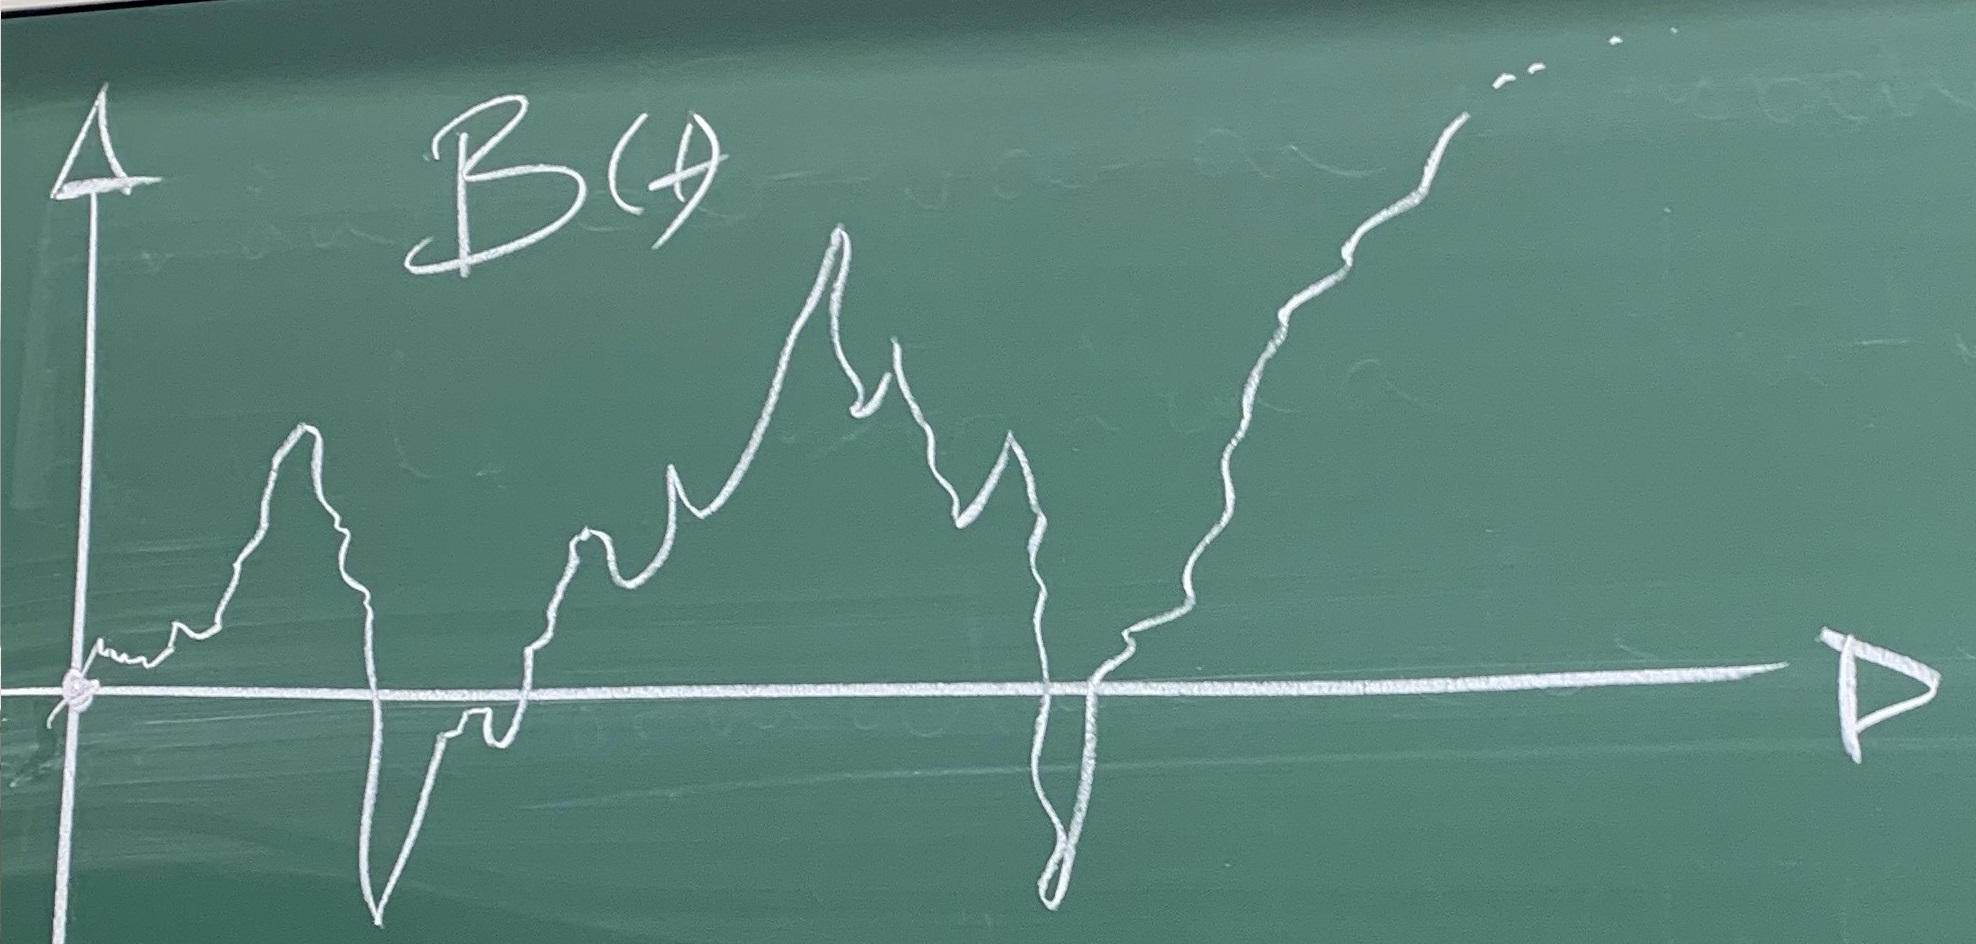
\includegraphics[scale=0.2]{lessons/lesson06/imgs/img04.jpg}\\
Browask rörelse används bland annat inom signalbehandling och inom
matematisk finans (för att modellera aktieprisutveckling).

\paragraph{Derivatan av trigonometriska funktioner}
\begin{itemize}
    \item $\frac{d}{dx}sin(x)=cos(x)$
    \item $\frac{d}{dx}cos(x)=-sin(x)$
    \item $\frac{d}{dx}tan(x)=\frac{1}{cos^2(x)}=\frac{1}{1-sin^2(x)}=\{\frac{cos^2(x)+sin^2(^x)}{cos^2(x)}\}=1+tan^2(x)$
\end{itemize}
Alla dessa bygger på beviset att $\lim_{x\to 0}\frac{sin(x)}{x}=1$

\paragraph{Ex} (2.4.12)
Beräkna derivatan av $f(x)=(2+|x|^3)^{\frac{1}{3}}$.
\subparagraph{Lösning}
Tänk på $2+|x|^3$ som en inre funktion och använd kedjeregeln!
\begin{equation*}
    f^\prime(x)=\frac{1}{3}\cdot (2+|x|^3)^{\frac{1}{3}-1}\cdot(2+|x|^3)^\prime=
    \frac{1}{3}(2+|x|^3)^{-\frac{2}{3}}\cdot(2+|x|^3)^\prime
\end{equation*}
Vad är derivatan av $2+|x|^3$?
\begin{equation*}
    (2+|x|^3)^\prime=0+(|x|^3)^\prime=
    3\cdot|x|^2\cdot(|x|)^\prime
\end{equation*}
Vad är $(|x|)^\prime$?
\begin{equation*}
    |x|=\left\lbrace\begin{matrix}
        x\text{, om } x\geq 0 \\
        -x\text{, om} x < 0
    \end{matrix}\right.
    \Rightarrow
    \underbrace{(|x|)^\prime=\left\lbrace\{\begin{matrix}
            1\text{, om } > 0 \\
            -1\text{, om } < 0
        \end{matrix}\right.}
\end{equation*}
$=sgn(x) \text{(sign function)}$

så $f^\prime(x)=\frac{1}{3}(2+|x|^3)^\frac{-2}{3}\cdot 3\cdot|x|^3\cdot sgn(x)=
    \frac{x^2}{(2+|x|^3)^\frac{2}{3}}\cdot sgn(x),x\neq 0$
Om en funktion $f$ beskriver hur värdet $y$ av någon typ av process beror av en inparameter $x$,
dvs. $y=f(x)$ så beskriver derivatan $f^\prime(x)$ hur snabbt eller långsamt motsvarande process förändras givet indata $x$.
$f^prime(x)$ kan tolkas som förändringshastigheten av $f$ i punkten $x$.

\paragraph{Ex}~\\
$x=$"Framlednings temperatur för radiatorvatten"\\
$f(x)=$"Inomhus temperatur givet framlednings temperatur $x$"\\
$\Rightarrow f^\prime(x)=$ "Förändringshastighet i inomhustemperetaur givet förändring i framledningstemperatur $x$".\\
\\Derivator används och tolkas på liknande sätt i en mängd olika sammanhang för ekonomi/samhällsvetenskap till fysik/teknik/naturvetenskap.

Måste förstå möjligheter, begränsningar och egenskaper för $f^\prime$.

\paragraph{Ex (2.7.20)} Bestäm förändringshastigheten för sidorna av en kub som funktion av kubens volym.
\subparagraph{Lösning} Kalla kubens sidlängd för $s$ och dess volym för $V$.\\
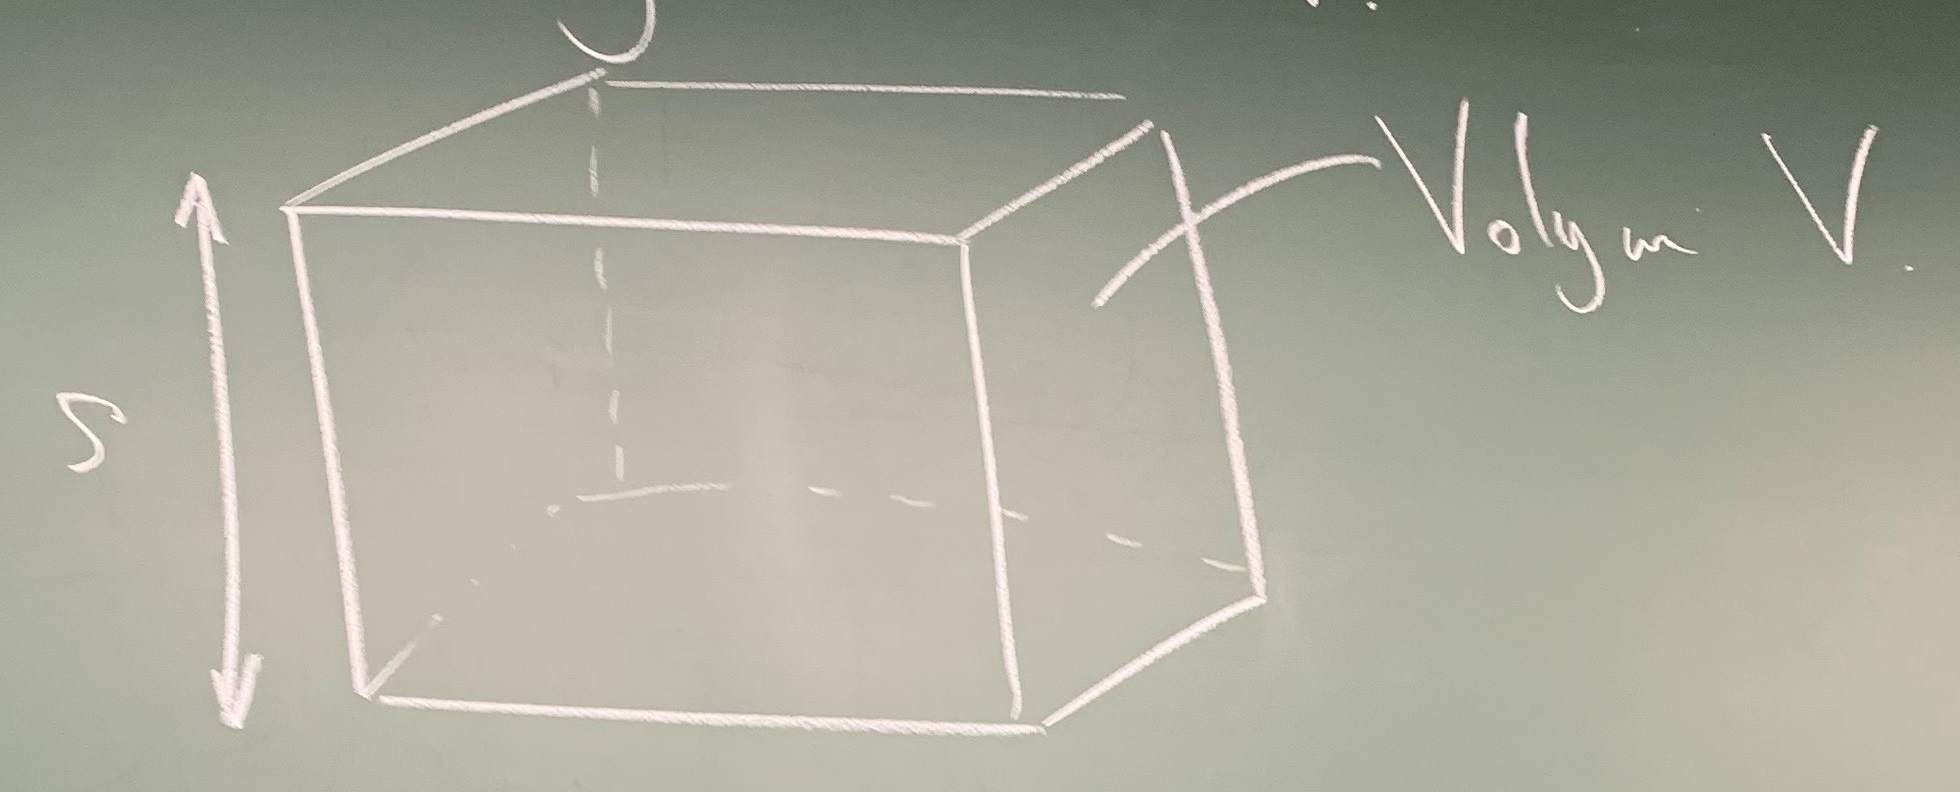
\includegraphics[scale=0.1]{lessons/lesson07/imgs/img01.jpg}\\
Vi villa hitta ett explicit uttryck för $s'(V)$.
Vet att $V=s^3\Leftrightarrow s=\sqrt[3]{V}=V^\frac{1}{3}$.
Alltså är $s'(V)=\frac{1}{3}\cdot V^{\frac{1}{3}-1}=\frac{1}{3}\cdot V=\frac{1}{3\cdot V^{\frac{2}{3}}}$ $\Box$

\paragraph{Ex (2.7.29)} Om det kostar en fabrikör $C(x)$ kr att tillverka $x$ enheter av något så innebär detta en snittkostnad per enhet av $\frac{C(x)}{x}$ (Kr/enhet).
Visa att det antal enheter $x$ som minimerar snittkostnaden gör snitt- och marginalkostnad lika (dvs $C^\prime(x)$).
\subparagraph{Lösning} Låt $A(x)$ beteckna snittkostnad. Dvs. $A(x)=\frac{C(x)}{x}$.\\
Då gäller att:
\begin{equation*}
    A^\prime(x)=\frac{d}{dx}[\frac{C(x)}{x}]=\{\text{prod.reg.}\}=C^\prime(x)\cdot x^{-1}+C(x)\cdot (-1)\cdot x^{-2}=\frac{C^\prime(x)\cdot x-C(x)}{x^2}
\end{equation*}
Vi ser att
\begin{equation*}
    A^\prime(x)=0\Leftrightarrow C^\prime(x)\cdot x-C(x)=0\Leftrightarrow\text{marginalkost.}=C^\prime(x)=\frac{C(x)}{x}=\text{snittkost. }\Box
\end{equation*}
Varför sattes $A^\prime(x)=0$ som en garant för att minimum?
Rent generellt så betyder $f^\prime(x_0)=0$ att en given funktion $f$ har horizontell tangent i $x=x_0$.
Sådana punkter $x=x_0$ kallas för \underline{kritiska punkter} och man säger att $f$ är \underline{stationär} för sådana $x$.
Geometriskt kan detta bara betyda något av följande:\\
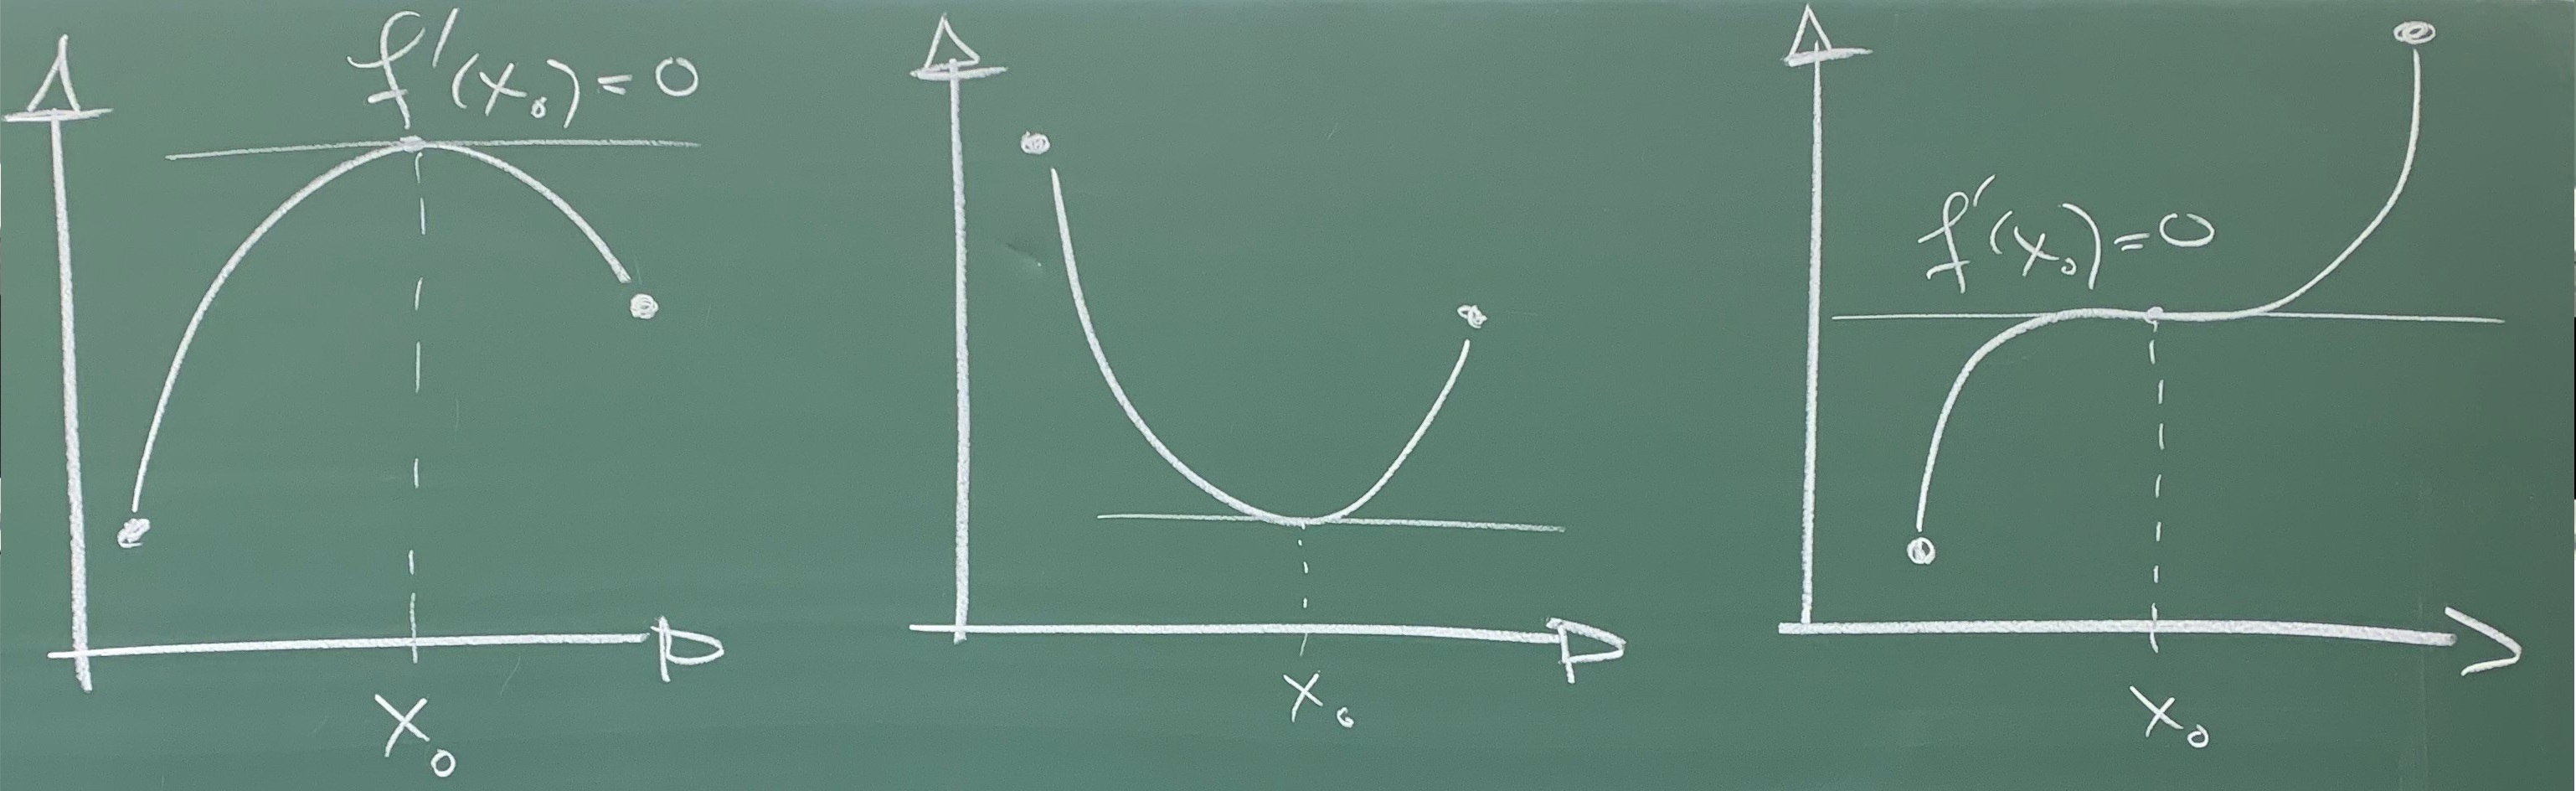
\includegraphics[scale=0.1]{lessons/lesson07/imgs/img02.jpg}\\
Hur visste man att $A^\prime(x)=0$ skulle motsvara en kritisk punkt flr ett minvärde av $A(x)$?
Rimligt att anta att $C(x)=K+c(x)$ där $K$ är en konstant, fast kostand, och $c(x)$ är enhetskostnaden
\begin{itemize}
    \item $A(x)\approx \frac{K}{x}$, om $x$ litet $\Rightarrow$ avtagande.
    \item $A(x)\approx \frac{c(x)}{x}$, om $x$ stort $\Rightarrow$ konstant eller växande.
\end{itemize}
$\Rightarrow A(x)$ har ett minimimum?\\
Smidigt att kika på högre ordning av derivator!\\
Givet en funktion $f$ kan man definiera \underline{andraderivatan} $f^{\prime\prime}$ som $^{\prime\prime}=(f^\prime)^\prime$.
På liknande sätt definieras tredje, fjärde och högre ordnings derivator som $f^{(n)}=((...(f^\prime)^\prime...))^\prime$.
andraderivatan bär precis som förstaderivatan både på teknisk- och geometrisk information om $f$.
Om $x=$tid och $f(x)=$tillryggalagd sträcka så motsvarar $f^\prime(x)$ momentanhastighet och $f^{\prime\prime}(x)$ momentanacceleration.
Geometriskt så kan $f^{\prime\prime}(x_0)$ tolkas som \underline{krökningen} av grafen till $f$ i punkten $x=x_0$.
Det gäller att om
\begin{itemize}
    \item $f^{\prime\prime}(x_0)>0\Rightarrow f$ \underline{konvex} i $x_0$
    \item $f^{\prime\prime}(x_0)<0\Rightarrow f$ \underline{konkav} i $x_0$
    \item $f^{\prime\prime}(x_0)=0\Rightarrow f$ kan vara konvex, konkav eller inget (och kan vara en så kallad \underline{inflektionspunkt}.)
\end{itemize}

Speciellt gäller för stationära punkter där $f^\prime(x_0)=0$ att:
\begin{itemize}
    \item $f^{\prime\prime}(x_0)>0\Rightarrow f$ har ett lokalt minimum i $x_0$
    \item $f^{\prime\prime}(x_0)<0\Rightarrow f$ har ett lokalt maximum i $x_0$
\end{itemize}

\paragraph{Sats} (Rolles sats)\\
Antag att $g$ är konstinuerlig på $[a,b]$ och deriverbar på $(a,b)$.
Om $g(a)=g(b)$ så finns en punkt $c\in(a,b)$ sådan att $g^\prime(c)=0$.
\subparagraph{Notera} Rolles sats är ett specialfall av medelvärdessatsen för derivator.

\paragraph{Sats} (Medelvärdessatsen för derivator) (tenta)\\
Antag att $f$ är en kontinuerlig funktion på $[a,b]$ och deriverbar på $(a,b)$.
Då existerar minst en punkt $c\in(a,b)$ sådan att $\frac{f(b)-f(a)}{b-a}=f^\prime(c)$.\\
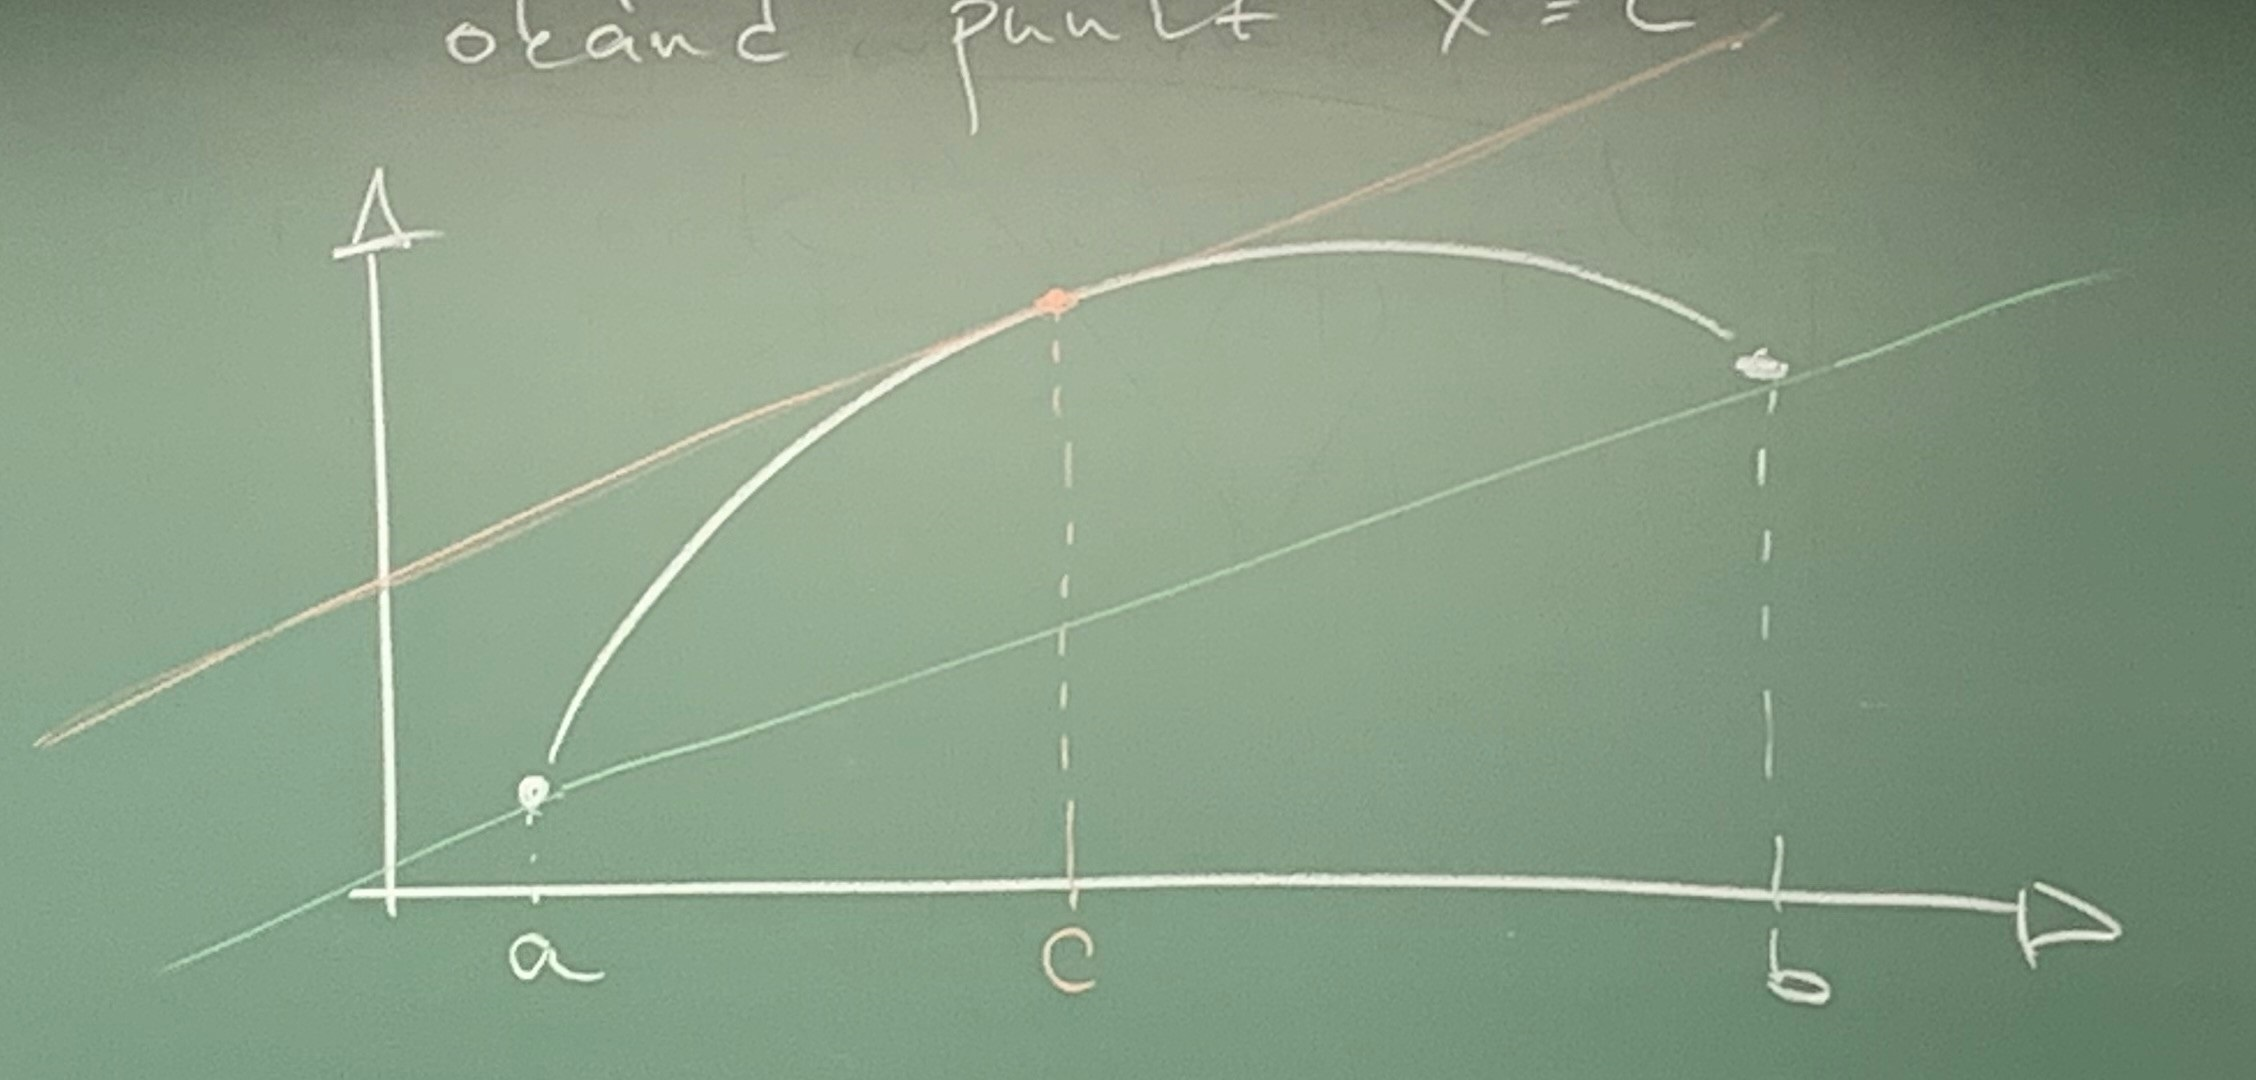
\includegraphics[scale=0.1]{lessons/lesson07/imgs/img03.jpg}\\
\subparagraph{Bevis}
Givet en funktion $f$ som uppfyller villkoren för satsen så kan vi konstruera funktionen $g$ som $g(x)=f(x)-(f(a)+\frac{f(b)-f(a)}{b-a})\cdot (x-a)$.
Uppenbart att $g$ är kontinuerlig på $[a,b]$ och deriverbar på $(a,b)$ då $f$ är det.
Alltså är $g(a)=g(b)$ och $g^\prime(x)=f^\prime(x)-0-\frac{f(b)-f(a)}{b-a}$.
Enligt Rolles sats finns då en punkt $c\in(a,b)$ så att $g^\prime(c)=f^\prime(c)-\frac{f(b)-f(a)}{b-a}$ $\Box$

\paragraph{Sats}
Låt $J$ vara ett öppet intervall och $I$ vara $J$ med eller utan ändpunkter.
Om $f$ är kontinuerlig på $I$ och deriverbar på $J$ gäller att:
\begin{itemize}
    \item $f^\prime(x)\begin{matrix}
                  > \\
                  <
              \end{matrix}\text{ }0\text{, }\forall x\in J \Rightarrow f \begin{matrix}
                  \text{strängt växande} \\
                  \text{strängt avtagande}
              \end{matrix}$ på $I$
    \item $f^\prime(x)\begin{matrix}
                  \geq \\
                  \leq
              \end{matrix}\text{ }0\text{, }\forall x\in J \Rightarrow f \begin{matrix}
                  \text{växande} \\
                  \text{avtagande}
              \end{matrix}$ på $I$
\end{itemize}
\section{Implicit derivering}
Att derivera en given funktion $f(x)$ är lätt med hjälå av regler som till exempel produktregeln och kedjeregeln.
Ibland vill man dock beräkna derivator för kurvor som \underline{inte} är funktionsgrafer,
till exempel\\
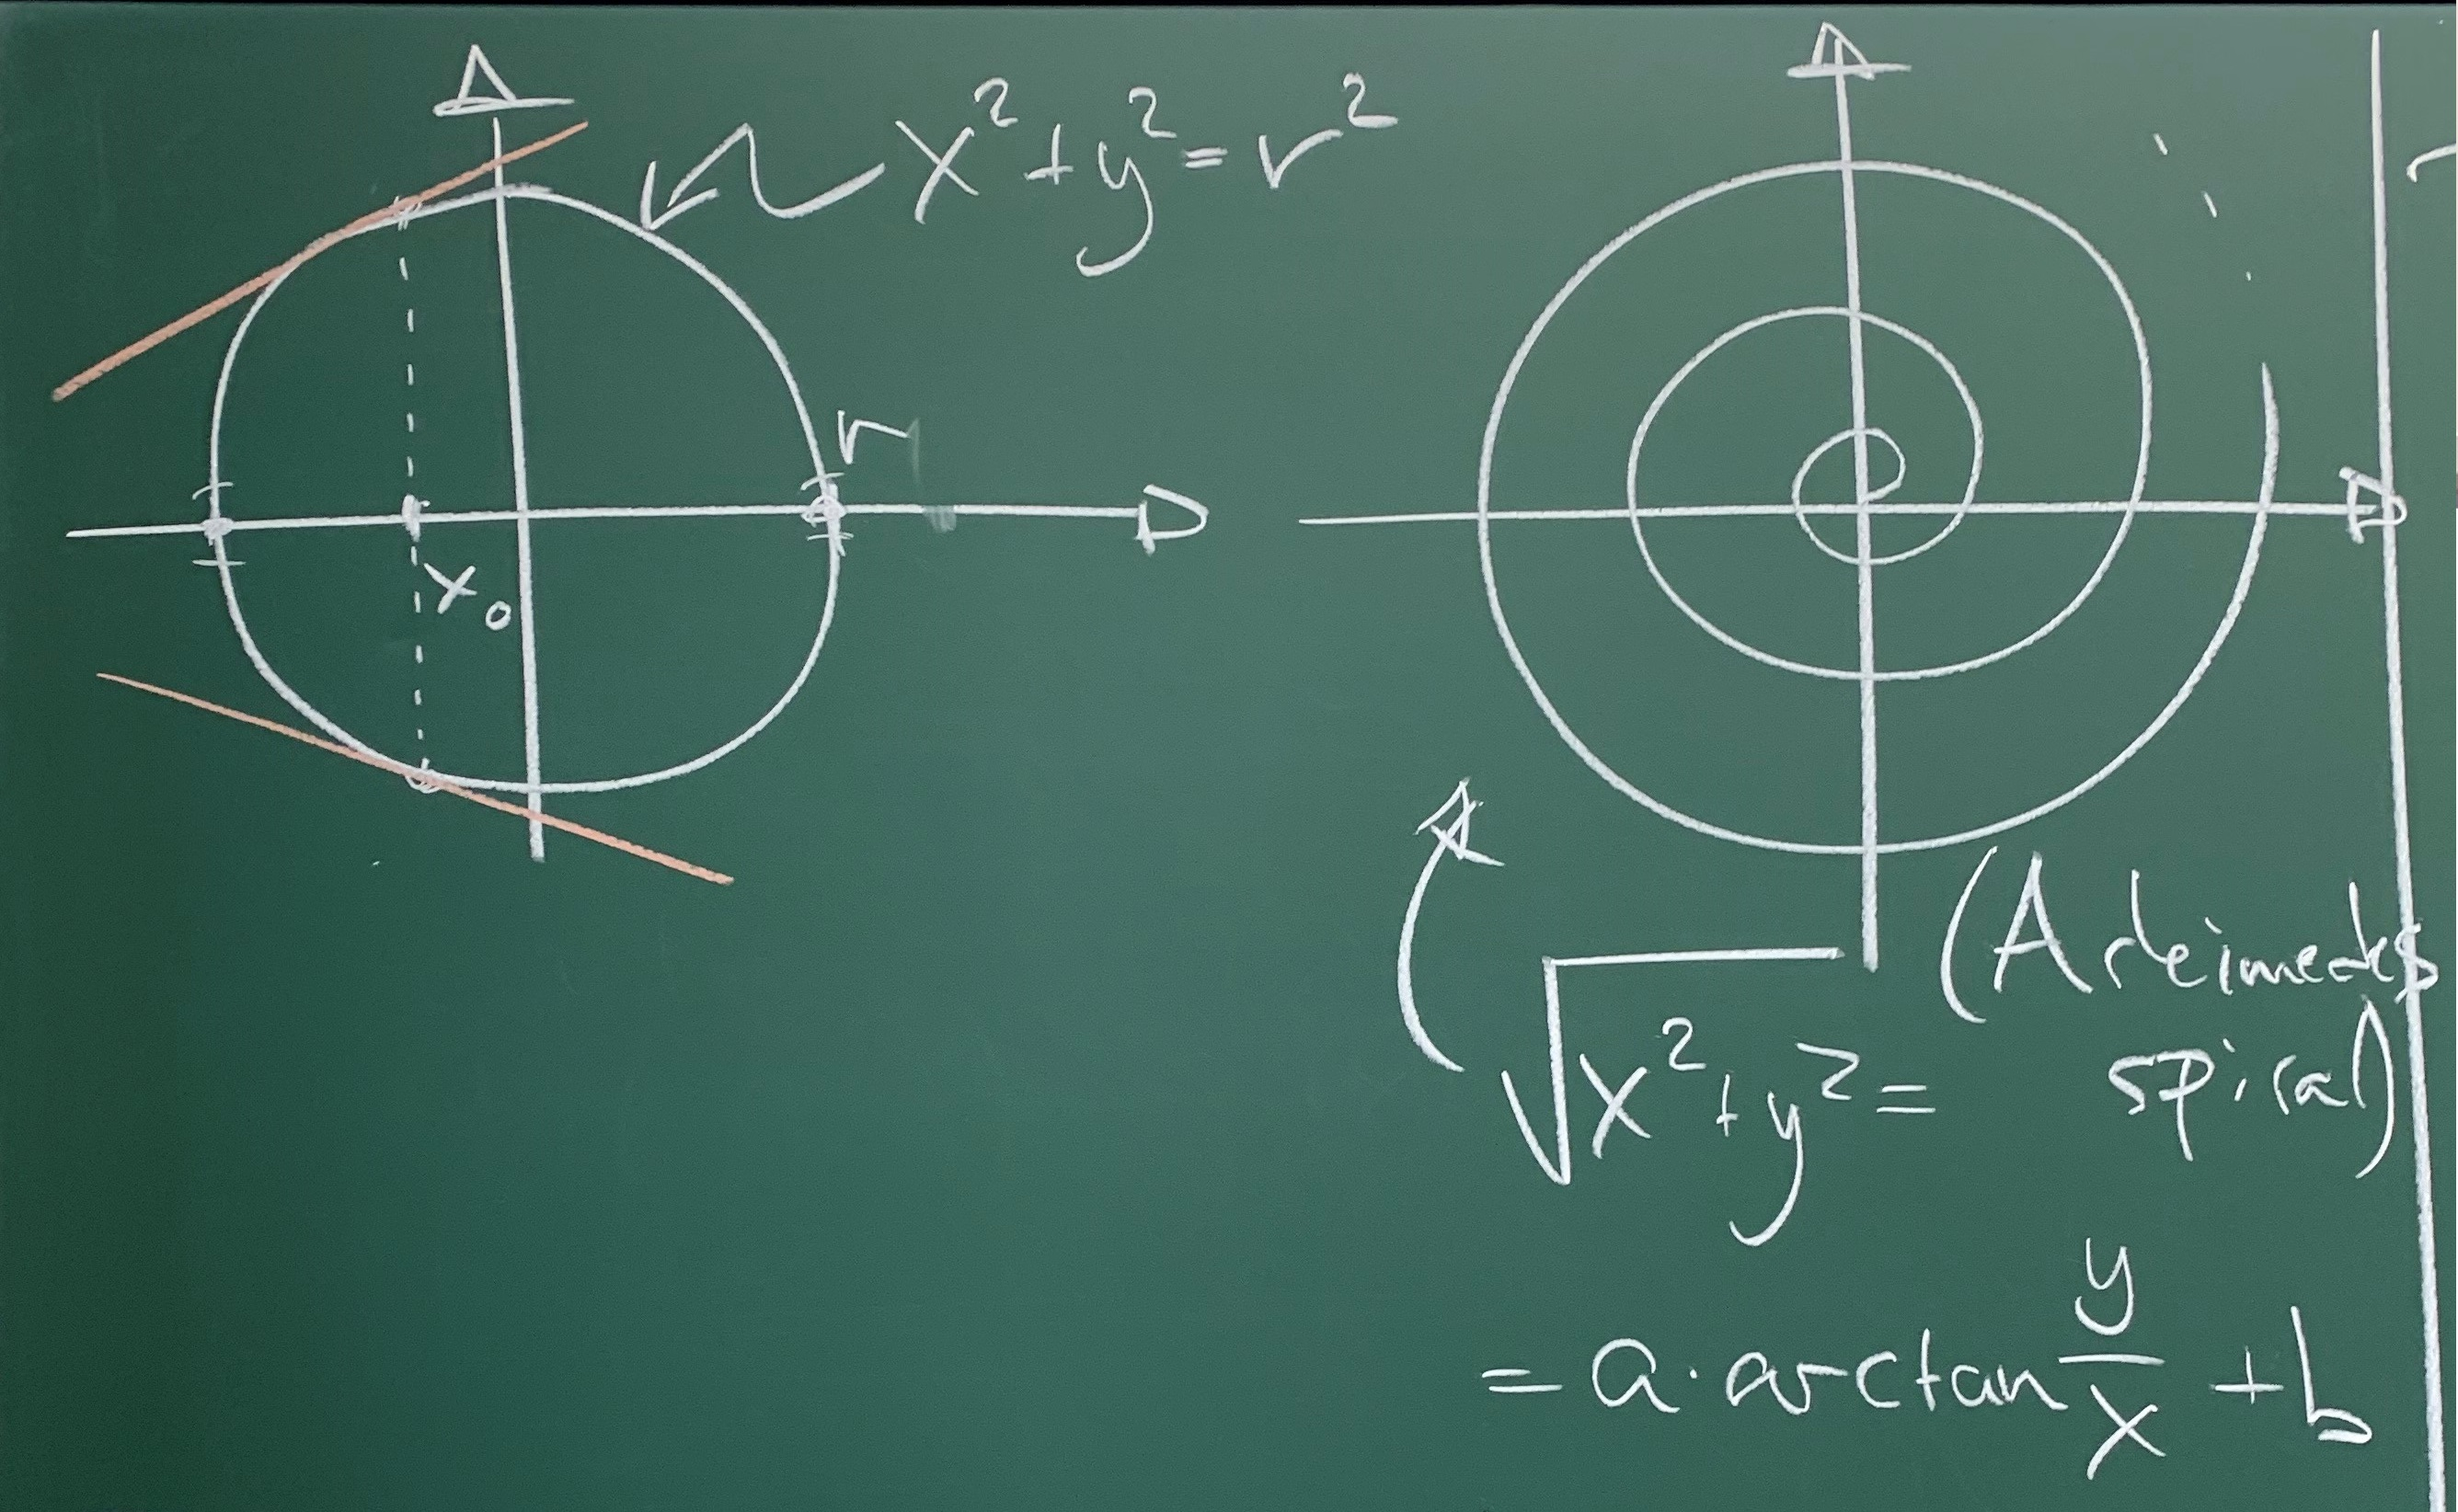
\includegraphics[scale=0.1]{lessons/lesson08/imgs/img01.jpg}\\
Denna typ av kurvor kan inte skrivas på formen $y=f(x)$,
men däremot som $F(x,y)=0$.

\paragraph{Ex} Archimedes spiral kan skrivas $F(x,y)=\sqrt{x^2+y^"}-a\cdot \arctan{\frac{y}{x}}-b$\\
\\
Hur beräknar man kurvan $F(x,y)=0$ i punkten $x=x_0$?
Notera att det mycket väl kan finnas \underline{flera} derivator tillhörande en given punkt $x=x_0$.
Man kan använda kedjeregeln för att beräkna $F^\prime(x,y)$.

\paragraph{Ex (2.9.5)} Givet kurvan $x^2y^3=2x-y$, bestäm $y^\prime$ uttryckt i termer av $x$ och $y$.
\subparagraph{Lösning}
\begin{equation*}
    x^2y^3=2x-y\Leftrightarrow F(x,y)=x^2y^3-2x+y=0
\end{equation*}
\begin{equation*}
    F^\prime(x,y)=\frac{d}{dx}[F(x,y)]=\frac{d}{dx}[x^2y^3-2x+y]=\frac{d}{dx}(x^2y^3)-\frac{d}{dx}(2x)+\frac{d}{dx}(y)=
\end{equation*}
\begin{equation*}
    \{\frac{d}{dx}(2x)=2,\frac{d}{dx}(y)=\frac{dy}{dx}=y^\prime\}=\frac{d}{dx}(x^2x^3)-2+y^\prime=\{\text{produktregeln}\}=
\end{equation*}
\begin{equation*}
    2x\cdot y^3+x^2\cdot\frac{d}{dx}(y^3)-2+y^\prime=\{\text{kedjeregeln}\}=2x\cdot y^3+x^2\cdot 3\cdot y^2\cdot y^\prime-2+y^\prime
\end{equation*}
För kurvan gäller att:
\begin{equation*}
    F(x,y)=0\Rightarrow F^\prime(x,y)=0\Rightarrow 2xy^3+3x^2y^2y^\prime-2+y^\prime=0\Leftrightarrow y^\prime=\frac{2-2xy^3}{1+3x^2y^2}\text{ }\Box
\end{equation*}
\\
Vid implicit derivering måste man vara noga med att ha koll på punkter där derivatan eventuellt inte existerar.

\chapter{Primitiva funktioner och indefinita integraler}
Med en primitiv funktion (antiderivata) till en funktion $f$ definierad på ett intervall $I$ menas \underline{en} funktion $F$ sådan att
\begin{equation*}
    F^\prime(x)=f(x)\text{ }\forall x\in I
\end{equation*}
Eftersom derivatan av alla konstantfunktioner är $g(x)=c$ är $0$ ($g^\prime(x)=0$) så finns oändligt många primitiva funktioner till $f$ eftersom alla $G(x)=F(x)+C$ funkar.
Den \underline{indefinita integralen} av $f$ innefattar alla dessa!

\paragraph{Definition} Givet en funktion $f$ definieras den indefinita integralen som $\int f(x),dx:=F(x)+C,x\in I$ där $C$ är en godtycklig konstant och $F$ är en primitivv funktion till $f$, dvs $F^\prime(x)=f(x)\forall x\in I$.
\\\\
Integraler är en hörnsten inom matematisk analys och anvönds i en mängd olika sammanhang.

\paragraph{Ex (2.10.30)} Lös begynnelseproblemet $\left\lbrace\begin{matrix}
        y^\prime=x^\frac{1}{3} \\
        y(0)=5
    \end{matrix}\right.$
\subparagraph{Lösning} Att lösa begynnelseproblemet innebär att bestämma $y(x)$.\\
Om $y^\prime=\frac{1}{3}$ så måste $y=\int x^\frac{1}{3}dx=\{\frac{4}{3}x^\frac{1}{3}\}=\frac{3}{4}x^\frac{4}{3}$.
Vidare så vet vi att $y(0)=5$ så $\Rightarrow \frac{3}{4}\cdot 0+c=5\Leftrightarrow C=5$ och vi får att $y=\frac{3}{4}x^\frac{4}{3}+5$ $\Box$

\chapter{L'Hôpital regler}
L'Hôpitals regeler är en strategi som ibland kan användas för att lösa icketriviala gränsvärdesproblem,
dvs gränsvärden av typen
\begin{equation*}
    \lim_{x\to ...}=\frac{"0"}{0},\frac{"\pm\infty"}{\pm\infty},"0\cdot\infty", "\infty-\infty"
\end{equation*}
L'Hôpitals regler kan funka för gränsvärden för de två första typerna.
Reglerna använder derivator!

\paragraph{L'Hôpitals första regel}~\\
Antag att $f$ och $g$ är deriverbara på $(a,b)$ och att $g^\prime(x)\neq 0$.
Antag också att
\begin{enumerate}
    \item $\lim_{x\to c}f(x)=\lim_{x\to c}g(x)=0,c\in(a,b)$
    \item $\lim_{x\to c}\frac{f^\prime(x)}{g^\prime(x)}=L$ (där $L$ kan vara ändligt eller oändligt)
\end{enumerate}
Då är $\lim_{x\to c}\frac{f(x)}{g(x)}=L$.\\
(Funkar även för $\lim_{x\to a^+},\lim_{x\to b^-}$ och om $a,b=\pm\infty$)

\paragraph{L'Hôpitals andra regel}~\\
Antag att $f$ och $g$ är deriverbara på $(a,b)$ ohc att $g^\prime(x)\neq 0$.
Antag också att
\begin{itemize}
    \item $\lim_{x\to c}g(x)=\pm\infty,c\in(a,b)$
    \item $\lim_{x\to c}\frac{f^\prime(x)}{g^\prime(x)}=L$ ($L$ är ändlig)
\end{itemize}
Då är gränsvärdet $\lim_{x\to c}\frac{f(x)}{g(x)}=L$.

\paragraph{Ex (4.3.6)} Bestäm $\lim_{x\to 1}\frac{x^\frac{1}{3}-1}{x^\frac{2}{3}-1}$
\subparagraph{Lösning} Gränsvärde av typen $"\frac{0}{0}"$.
Om $f(x)=x^\frac{1}{3}-1$ och $g(x)=x^\frac{2}{3}-1$ så är $g^\prime(x)=\frac{2}{3}x^{-\frac{1}{3}}$ och därmed $g^\prime(x)\neq 0$ i en omgivning av $x=1$,
dvs $(1-\varepsilon,1+\varepsilon)$ för $\varepsilon>0$.
Gäller också att $\lim_{x\to 1}f(x)=\lim_{x\to 1}g(x)=0$ och att
\begin{equation*}
    \lim_{x\to 1}\frac{f^\prime(x)}{g^\prime(x)}=\lim_{x\to 1}\frac{\frac{1}{3}x^\frac{-2}{3}}{\frac{2}{3}x^\frac{-1}{3}}=\lim_{x\to 1}\frac{1}{3}x^\frac{-2}{3}\frac{3}{2}x^\frac{1}{3}=\lim_{x\to 1}\frac{1}{2}x^\frac{-1}{3}=\frac{1}{2}
\end{equation*}
och enligt L'Hôpitals första regel gäller att
\begin{equation*}
    \lim_{x\to 1}\frac{x^\frac{1}{3}-1}{x^\frac{2}{3}-1}=\frac{1}{2}\text{ }\Box
\end{equation*}

\chapter{Standardgränsvärden}
Förutom L'Hôpitals regeler finns en samling Standardgränsvärden som man
\underline{alltid} kan ta för givna (om inte annat anges) när man löser gränsvärdesproblem.
\begin{itemize}
    \item $\lim_{x\to 0}\frac{\sin(x)}{x}=1$
    \item $lim_{x\to \infty}\frac{x^b}{a^x}=0$, om $a>1$ och $b\in\mathbb{R}$
    \item $\lim_{n\to \infty} \sqrt[n]{a}=1$, om $a>0$
    \item $\lim_{n\to \infty} \sqrt[n]{n}=1$
\end{itemize}
\chapter{Funktioner}
För ala reella tall $a\neq 0$ gäller att $a\cdot \frac{1}{a}=1$.
Talet $1/a$ kallas för den \emph{multiplikativa inversen} till $a$.
Den multiplikativa inversen definieras med hjälp av det speciellt talet 1 (ettan) som har den \emph{unika} egenskapen att $a\cdot 1 = 1\cdot a=a$ $\forall a\in \mathbb{R}$.
Om vi istället för de reella talen nu tänker oss funktioner och istället för multiplikation tänker oss komposition, alltså $f\circ g$, finns det då en "etta"?
Ja! Funktionen $e(x)=x$ blir en etta eftersom $f\circ e(x)=f(e(x))=f(x)$ och $e\circ f(x)=e(f(x))=f(x)$ så alltså gäller att $f\circ e=e\circ f=f$ för alla funktioner $f$.
Med $e(x)=x$ som "etta" är det naturligt att fråga sig; givet en funktion $f$, finns det då en annan funktion $g$ så att $f\circ g=g\circ f=e$?
Ja! Funktionen $g(x)=\frac{1}{f(x)}$ blir en sådan funktion eftersom $f\circ g(x)=f(\frac{1}{f(x)})=\frac{1}{f(x)}$ och $g\circ f(x)=\frac{1}{f(f(x))}=\frac{1}{f(x)}$ så alltså gäller att $f\circ g=g\circ f=e$.
Detta gäller dock endast om $f$ är injektiv, alltså om $x_1\neq x_2\Rightarrow f(x_1)\neq f(x_2)$.
Funktionen $g$ kallas då för \emph{inversen} till $f$ och skrivs $f^{-1}$.
Geometriskt så representeras $f^{-1}$ som en spegelbild av $f$ i linjen $y=x$.
Lite grundläggande egenskaper för inverser:
\begin{itemize}
    \item $y=f^{-1}(x) \Leftrightarrow x=f(y)$
    \item $f\circ f^{-1}=f^{-1}\circ f=x$
    \item $(f^{-1})^{-1}(x)=f(x)$
\end{itemize}
Man kan också beräkna derivata av inversfunktionen som $\frac{d}{dx}(f^{-1}(x))=\frac{1}{f'(f^{-1}(x))}$
eftersom vi vet att $f(f^{-1}(x))=x\Rightarrow \frac{d}{dx}(f(f^{-1}(x)))=\frac{d}{dx}(x)=1$ och $\frac{d}{dx}(f(f^{-1}(x)))=$ \{kedjeregeln\} $=f'(f^{-1}(x))\cdot \frac{d}{dx}f^{-1}x\Rightarrow \frac{d}{dx}f^{-1}(x)=\frac{1}{f'(x^{-1}(x))}$.
\emph{Behöver inte bevisas på tentan.}
\section{Exponentialfunktioner}
En exponentialfunktion är en funktion på formen $f(x)=a^x$ där $a>0$.
Det gäller att $a^0=1$, $a^{x+y}=a^x\cdot a^y$, $a^{-x}=\frac{1}{a^x}$ och $(a^x)^y=a^{x\cdot y}$.
Vidare är funktionen $f(x)=a^x$ en \emph{injektiv} funktion, och därmed finns alltid en invers.
Denna invers kallas för \emph{$a$-logaritmen} och skrivs $f^{-1}(x)=\log_a(x)$.
För alla $a$-logaritmer gäller att
\begin{itemize}
    \item $y=\log_a(x) \Leftrightarrow x=a^y$
    \item $\log(1)=0$
    \item $\log_a(x\cdot y)=\log_a(x)+\log_a(y)$
    \item $\log_a(\frac{x}{y})=\log_a(x)-\log_a(y)$
    \item $\log_a(\frac{1}{x})=-\log_a(x)$
    \item $\log_a(x^y)=y\cdot \log_a(x)$
    \item $\log_a(x)=\frac{\log_b(x)}{\log_b(a)}$, om $a>0$ och $b>0$
\end{itemize}
Derivatan av $f(x)=a^x$ är $f'(x)=a^x\cdot \log_a(x)$.
Finns det ett tall $a$ så att $C=1$?
Ja, och det kallas $e\approx 2,718281828\ldots$.
Motsvarande $e$-logaritmen kallas för den \emph{naturliga logaritmen} och betecknas $\ln(x)$.
Genom detta fås att $\frac{d}{dx}a^x=\frac{d}{dx}e^{\ln(a^x)}=\frac{d}{dx}e^{x\cdot\ln(a)}=\ln(a)\cdot a^x$.
På motsvarande sätt gäller att $\frac{d}{dx}\ln(x)=\frac{1}{x}$, och $\frac{d}{dx}\log_a(x)=\frac{1}{x\cdot \ln(a)}$.
Exponentialfunktioner och logaritmer är oumbärliga för att modellera en mängd olika processer.
I synnerhet tillväxt-/avtagande-modellering.
\begin{figure}[h]
    \centering
    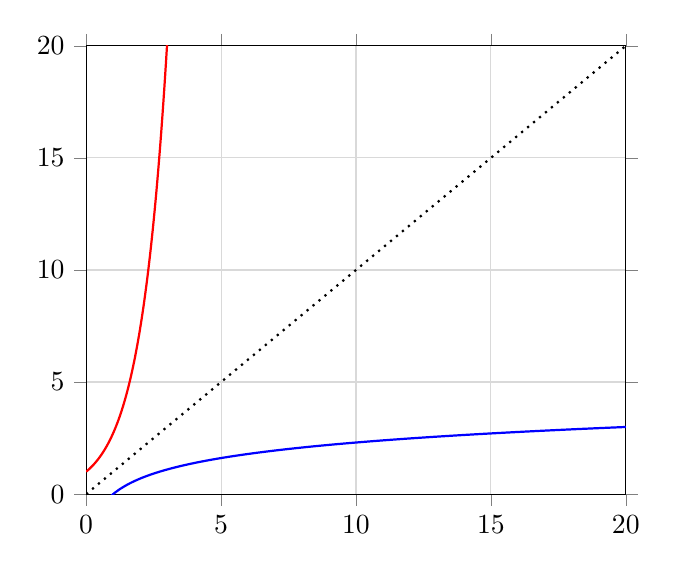
\begin{tikzpicture}
        \begin{axis}[
                xmin=0, xmax=20,
                xticklabel style={/pgf/number format/.cd,fixed},
                grid = major,
                grid style={gray!30},
                ymin=0,
                ymax= 20,
                axis background/.style={fill=white},
                tick align=outside
            ]
            \addplot[domain=0:3.5, red, thick, samples=200] {e^x};
            \addplot[domain=0.1:20, blue, thick, samples=200] {ln(x)};
            \addplot[domain=0:20, black, thick, dotted] {x};
        \end{axis}
    \end{tikzpicture}
    \caption{Kurvorna $y=e^x$ och $y=\ln(x)$}
\end{figure}
Jämfört med potensfunktionen $x^n$, $n>0$, så växer/avtar $e^x$ alltid snabbare och tvärtom för $\ln(x)$:
$\lim_{x\to \infty}\frac{x^n}{e^x}=0$, $\lim_{x\to -\infty}|x^n|e^x=0$, $\lim_{x\to\infty}\frac{\ln x}{x^n}=0$, $\lim_{x\to 0^+}x^n\cdot \ln x=0$.
Vad gäller för de primitiva funktionerna (indefinita integralerna) av $e^x$ och $\ln(x)$?
$\int e^x dx=e^x+C$, $\int \ln(x)dx=x\ln(x)-x+C$ (primitiv av $\ln(x)$ kan vi egentligen inte än).
För $\ln |x|$ gäller att $\frac{d}{dx}\ln |x|=\frac{1}{x}\cdot sgn(x)=\frac{1}{x}$, så $\int \frac{1}{x}dx=\ln |x|+C$.
Talet $e$ är intressant i sig, och omgärdas än idag av flera olösta matimatiska problem.
Det kan formuleras som följande kända gränsvärde: $e=\lim_{x\to\infty}(1+\frac{1}{n})^n$ och således gäller att $e^x=\lim_{x\to\infty}(1+\frac{x}{n})^n$.
\section{Inversa trigonometriska funktioner}
Funktionerna $\sin x$, $\cos x$ och $\tan x$ är periodiska och därmed inte injektiva på $\mathbb{R}$.
Av den anledningen saknas inversfunktioner.
Det går dock att begränsa dem så att de blir injektiva på ett kortare intervall.
$\arcsin x$, $\arccos x$ och $\arctan x$ har följande definitions- och värdemängder:
\begin{itemize}
    \item $\arcsin x$ $\mathcal{D}=[-1,1]$, $\mathcal{R}=[-\frac{\pi}{2},\frac{\pi}{2}]$
    \item $\arccos x$ $\mathcal{D}=[-1,1]$, $\mathcal{R}=[0,\pi]$
    \item $\arctan x$ $\mathcal{D}=[-\infty,\infty]$, $\mathcal{R}=[-\frac{\pi}{2},\frac{\pi}{2}]$
\end{itemize}
Man har följande derivator:
\begin{itemize}
    \item $\frac{d}{dx} \arcsin x=\frac{1}{\sqrt{1-x^2}}$
    \item $\frac{d}{dx} \arccos x=\frac{1}{\sqrt{1-x^e}}$
    \item $\frac{d}{dx} \arctan x=\frac{1}{1+x^2}$
\end{itemize}
\section{De hyperboliska funktionerna}
Släktingar till de trigonometriska funktionerna med många liknande egenskaper.
$\sinh x = \frac{e^x-e^{-x}}{2}$, $\cosh x = \frac{e^x+e^{-x}}{2}$
Precis som för $\sin$ och $\cos$, så är $\sinh$ en udda funktion och $\cosh$ en jämn funktion.
Den trigonometriska ettan gäller nästan (hyperboliska ettan!): $\cosh^2 x - \sinh^2 x = 1$.
För derivatorna gäller att $\frac{d}{dx}\sinh x = \cosh x$, $\frac{d}{dx}\cosh x = \sinh x$.
Man definierar $\tanh = \frac{\sinh}{\cosh}$och får att $\frac{d}{dx}$
\paragraph{Ex (4.1.11)} Hur snabbt förändras volymen av en rektangulär
låda då höjden är $6$ cm, bredden är $5$ cm och djupet är $4$ cm om både
höjd och djup ökar med $1$ cm/s och bredden minskar med $2$ cm/s?
\subparagraph{Lösning} Rita!\\
%infoga bild 1
%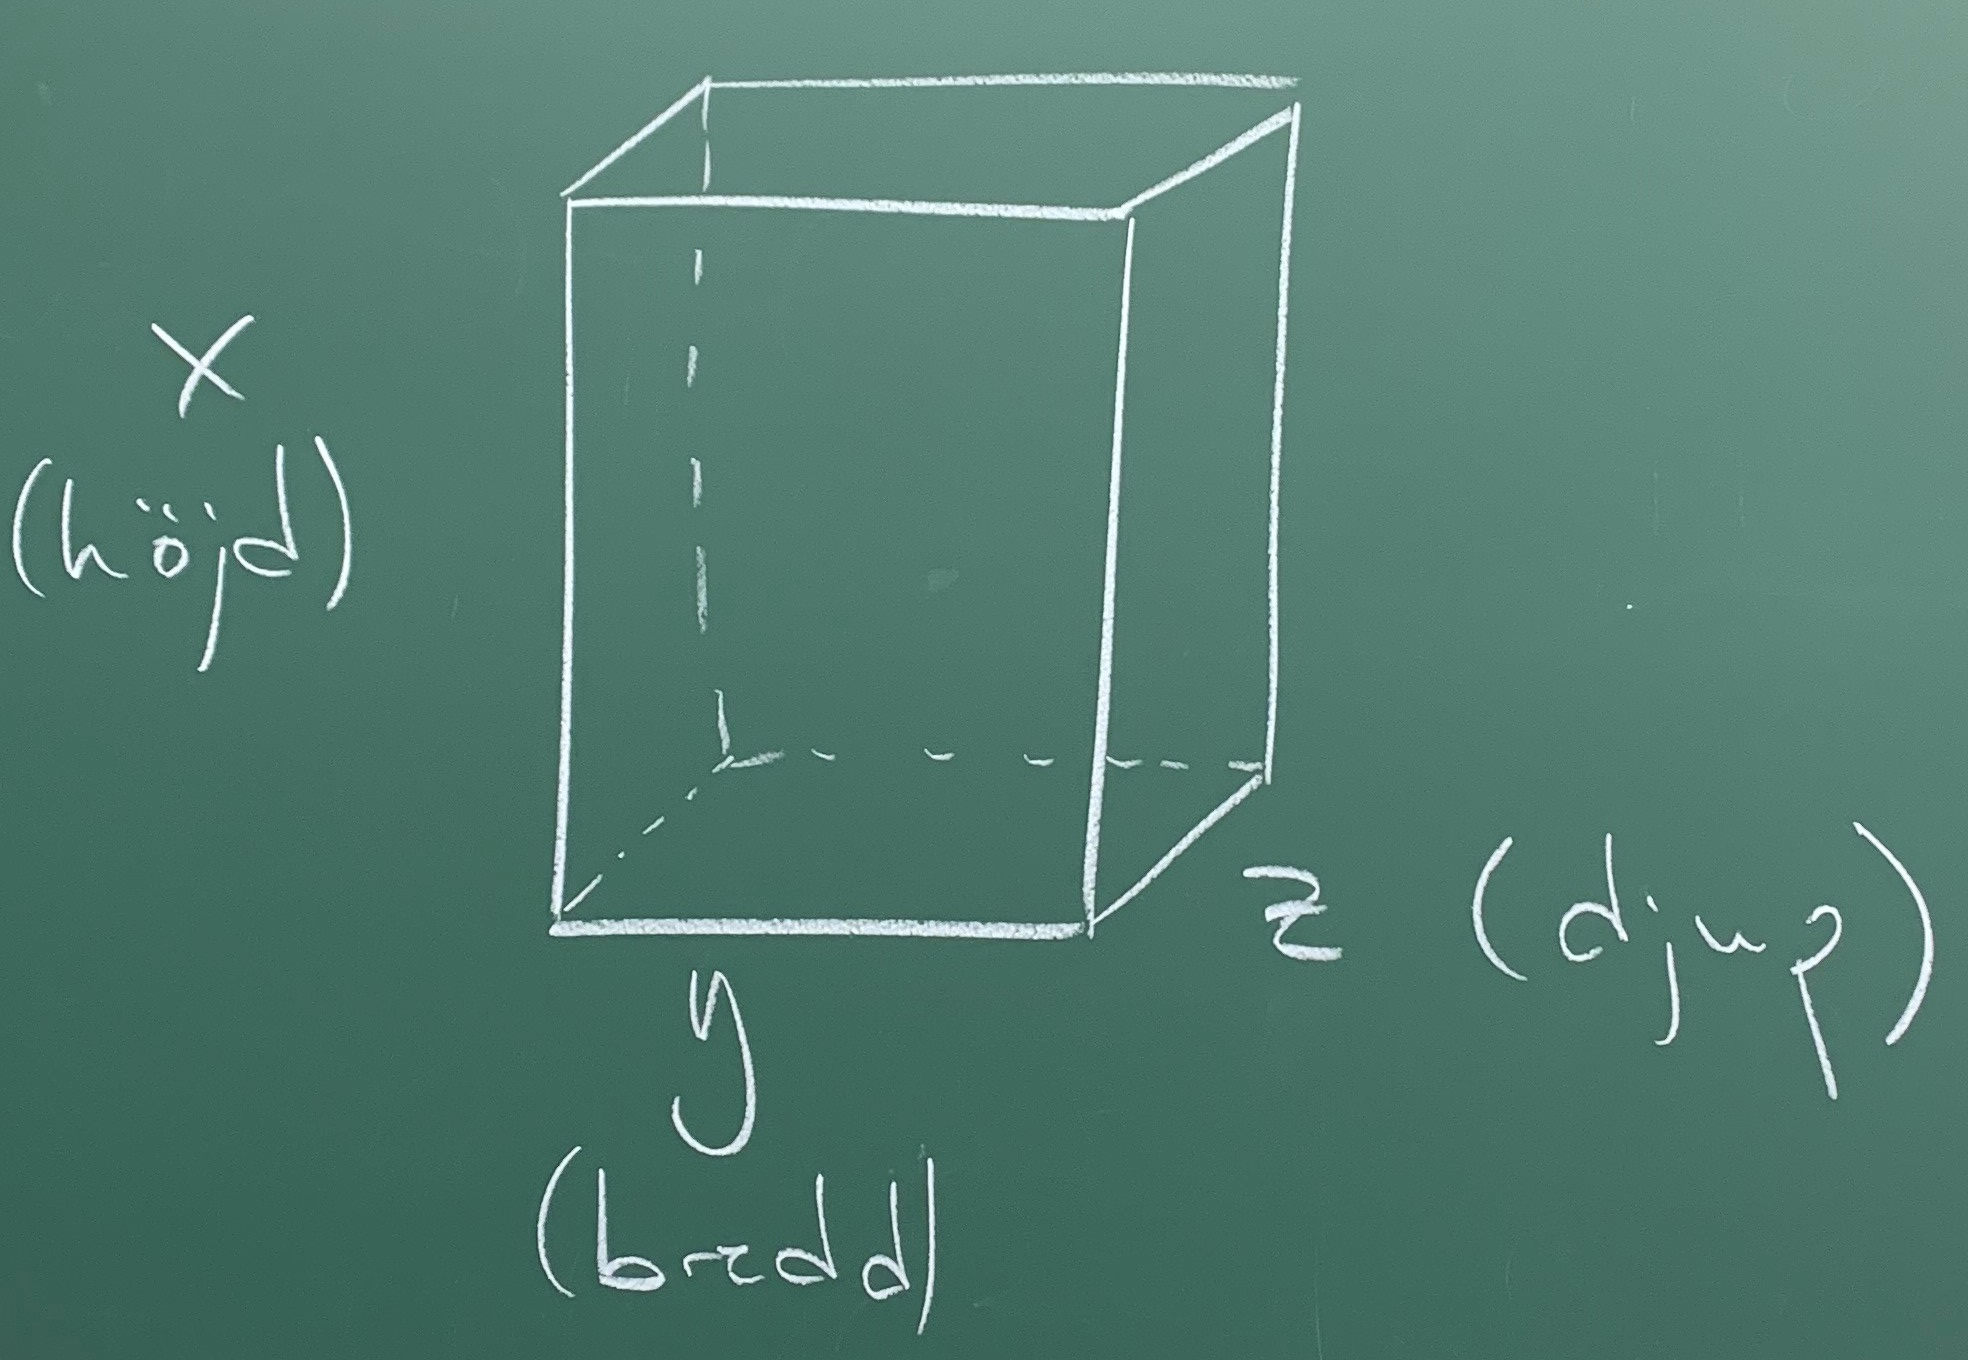
\includegraphics[scale=0.1]{lessons/lesson10/imgs/img01.jpg}\\
Lådans dimensioner beror av tiden så $x=x(t)$, $y=y(t)$ och $z=z(t)$.
Det gäller för volymen $V(t)$ att $V(t)=x(t)\cdot y(t)\cdot z(t)$
och vid tiden $t=t_0$ vet vi att $x(t_0)=6,y(t_0)=5,z(t_0)=4,x^\prime(t_0)=<^\prime(t_0)=1$ och $y^\prime(t_0)=-2$.
Vad blir $V^\prime(t_0)$?
\begin{equation*}
    V^\prime(t)=\frac{d}{dt}(x(t)\cdot y(t)\cdot z(t))=
    \{\text{prod.regeln}\}=
\end{equation*}
\begin{equation*}
    x^\prime(t)\cdot y(t)\cdot z(t) + x(t)\cdot y^\prime(t)\cdot z(t) + x(t)\cdot y(t)\cdot z^\prime(t)
    \Rightarrow V^\prime(t_0)=
\end{equation*}
\begin{equation*}
    1\cdot 5\cdot 4 + 6\cdot (-2)\cdot 4 + 6\cdot 5 \cdot 1=
    20-48+30=2\text{ cm}^3\text{/s}
\end{equation*}
så lådans volym \underline{ökar} med $2$ cm$^3$/s $\Box$

\paragraph{Ex (4.1.38)} Två tunga lådor är sammankopplade med ett $15$ m långt och starkt (icke-elastiskt) rep enligt figur\\
%infoga bild 2
%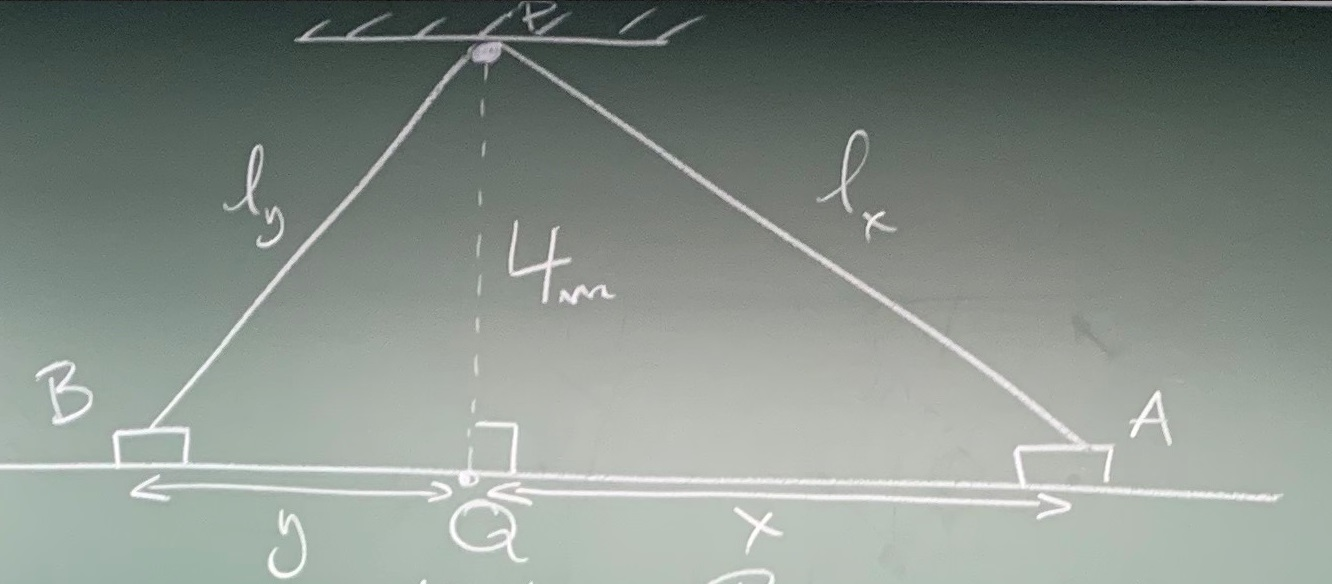
\includegraphics[]{lessons/lesson10/imgs/img02.jpg}\\
Hur snabbt rör sig låda $B$ mot punkten $Q$ då låda $A$ befinner sig $3$ m
från $Q$ och rör sig bort från denna punkt med en fart av $0.5$ m/s?
\subparagraph{Lösning}
Beteckna repets längd $l$ och de båda dellängderna $l_x$ och $l_y$.\\
Då gäller att:
$l(t)=l_x(t)+l_y(t)=\sqrt{x^2(t)+4^2}+\sqrt{y^2(t)+4^2}$ och
\begin{equation*}
    0=l^\prime(t)=\frac{1}{2}(x^2(t)+16)^{-\frac{1}{2}}\cdot 2x(t)\cdot x^\prime(t)+\frac{1}{2}(y^2(t)+16)^{-\frac{1}{2}}\cdot 2y(t)\cdot y^\prime(t)=
\end{equation*}
\begin{equation*}
    \frac{x(t)\cdot x^\prime(t)}{\sqrt{x^2(t)+16}}+\frac{y(t)\cdot y^\prime(t)}{\sqrt{y^2(t)+16}}
\end{equation*}
Vi vet att vid $t=t_0$ så är $x(t_0)=3,x^\prime(t_0)=0.5$ och \\
$y(t_0)=\sqrt{l_y^2-16}=\sqrt{(l-l_x)^2-16}=\sqrt{(15-\sqrt{16-9})^2-16}=\sqrt{84}$så \\
$0=\frac{3\cdot 0.5}{\sqrt{9+16}}+\frac{\sqrt{84}\cdot y^\prime(t_0)}{\sqrt{84+16}}\Rightarrow y^\prime(t_0)=-\frac{3}{\sqrt{84}}\approx -0.327\text{m/s }\Box$

\chapter{Numerisk ekvationslösning}
Handlar om att på numerisk väg lösa ekvationen $f(x)=0$.
Om till exempel $f$ är kontinuerlig kan man anvönda \underline{bisektionsalgoritmen}, dvs. hitta två tal $a$ och $b$ så att $f(a)<0$ och $f(b)>0$ (eller tvärt om!).
Då ligger åtminstone ett nollställe mellan $a$ och $b$.
Beräkna $f(\frac{a+b}{2})$, dvs. värdet i mittpunkten och avgör sedan om nollställe ligger i antingen intervallet $[a,\frac{a+b}{2}]$ eller i $[\frac{a+b}{2}, b]$.
Fortsätt på samma vis i delintervallen\dots

\paragraph{Fixpunktsiteration} Formulera om $f(x)=0$ som $g(x)=x$ (om möjligt).
Till exempel $f(x)=3\sin^2(x)+x^2-x=0$ blir då $g(x)=3\sin^2(x)+x^2=x$.
Tag sedan ett tal $x=x_0$ som troligtvis ligger nära det $x$ som löser ekvationen och sätt in i $g(x)$.
$x_0\rightarrow g(x_0)=x_1\rightarrow g(x_1)=x_2\rightarrow g(x_2)...$ dvs. beräkna $x_0,x_1,x_2,...$ enligt $g(x_n)=x_{n+1}$.
Under vissa förutsättningar konvergerar talföljden $\lim_{n\to\infty}x_n$ och man hittar en lösning till $g(x)=x$ dvs. $f(x)=0$.
Gränsvärdet $lim_{n\to\infty}x_n=x$ kallas \underline{fixpunkt} till $g(x)$.

\paragraph{Sats} Antag att $g$ är definierad på intervallet $I=[a,b]$ och uppfyllet att:
\begin{enumerate}
    \item $f(x)\in I$ om $x\in I$
    \item Det finns en konstant $0<k<1$ så att för att $u,v\in I$ gäller att $|f(u)-f(v)|\leq k\cdot|u-v|$ (lipschitz-kontinuitet).
          Då har $g$ en unik fixpunkt $r\in I$, dvs. $g(r)=r$, och oavsett val av $x_0\in I$ så är $\lim_{n\to\infty}x_n=r$.
\end{enumerate}

\paragraph{Newtons metod} Funkar bra om man söker nollställen $f(x)=0$ där $f$ är en deriverbar funktion.
Går ut på att iterativt hitta nollställen till tangentlinjer!\\
%infoga bild 3
%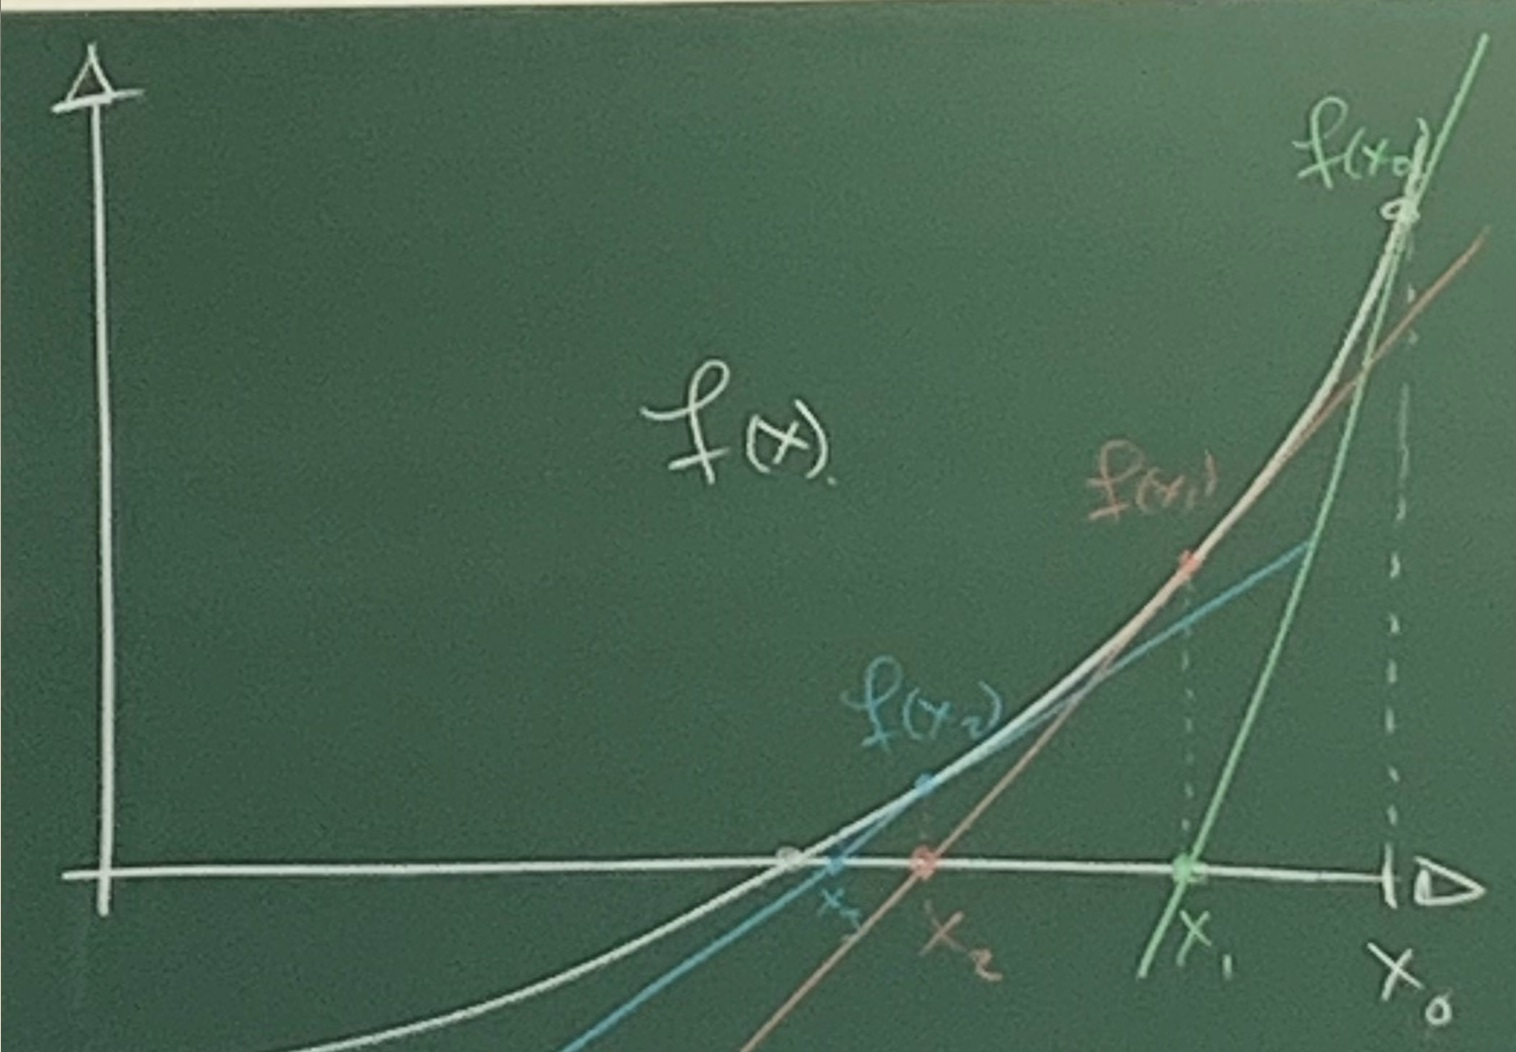
\includegraphics[scale=0.1]{lessons/lesson10/imgs/img03.jpg}\\
För $x=x_n$ har man tangentlinjen $\frac{y-f(x_n)}{x-x_n}=f^prime(x_n)$ och nollstället till denna ges av $\frac{0-f(x_n)}{x_{n+1}-x_n}=f^\prime(x_n)$ dvs $x_{n+1}=x_n-\frac{f(x_n)}{f^\prime(x_n)}$.
Newtons metod kan fallera om $f$ inte ör överallt deriverbar eller om det finns horizontella/vertikala tangenter.

\chapter{Extremvärden}
Ett extremvärde av en funktion $f$ är en punkt där värdet av $f$ är \\
maximalt/minimalt, antingen globalt eller lokalt.

\paragraph{Definition (globalt extremvärde)} En funktion $f$ har ett eller flera globalt maximum/minimum i $x=x_0$ (där $x_0\in D(f)$) om $f(x)\begin{matrix}\geq\\\leq\end{matrix}f(x_0)$ för alla $x\in D(f)$.

\paragraph{Definition (lokalt extremvärde)} En funktion $f$ har ett lokalt \\
maximum/minimum i $x=x_0$ (där $x_0\in D(f)$) om det finns ett tal $h>0$ så att $f(x)\begin{matrix}\geq\\\leq\end{matrix} f(x_0)$ för att $x\in D(f)$ så att $|x-x_0|<h$.\\
I en bild:\\
%ingoga bild 4
%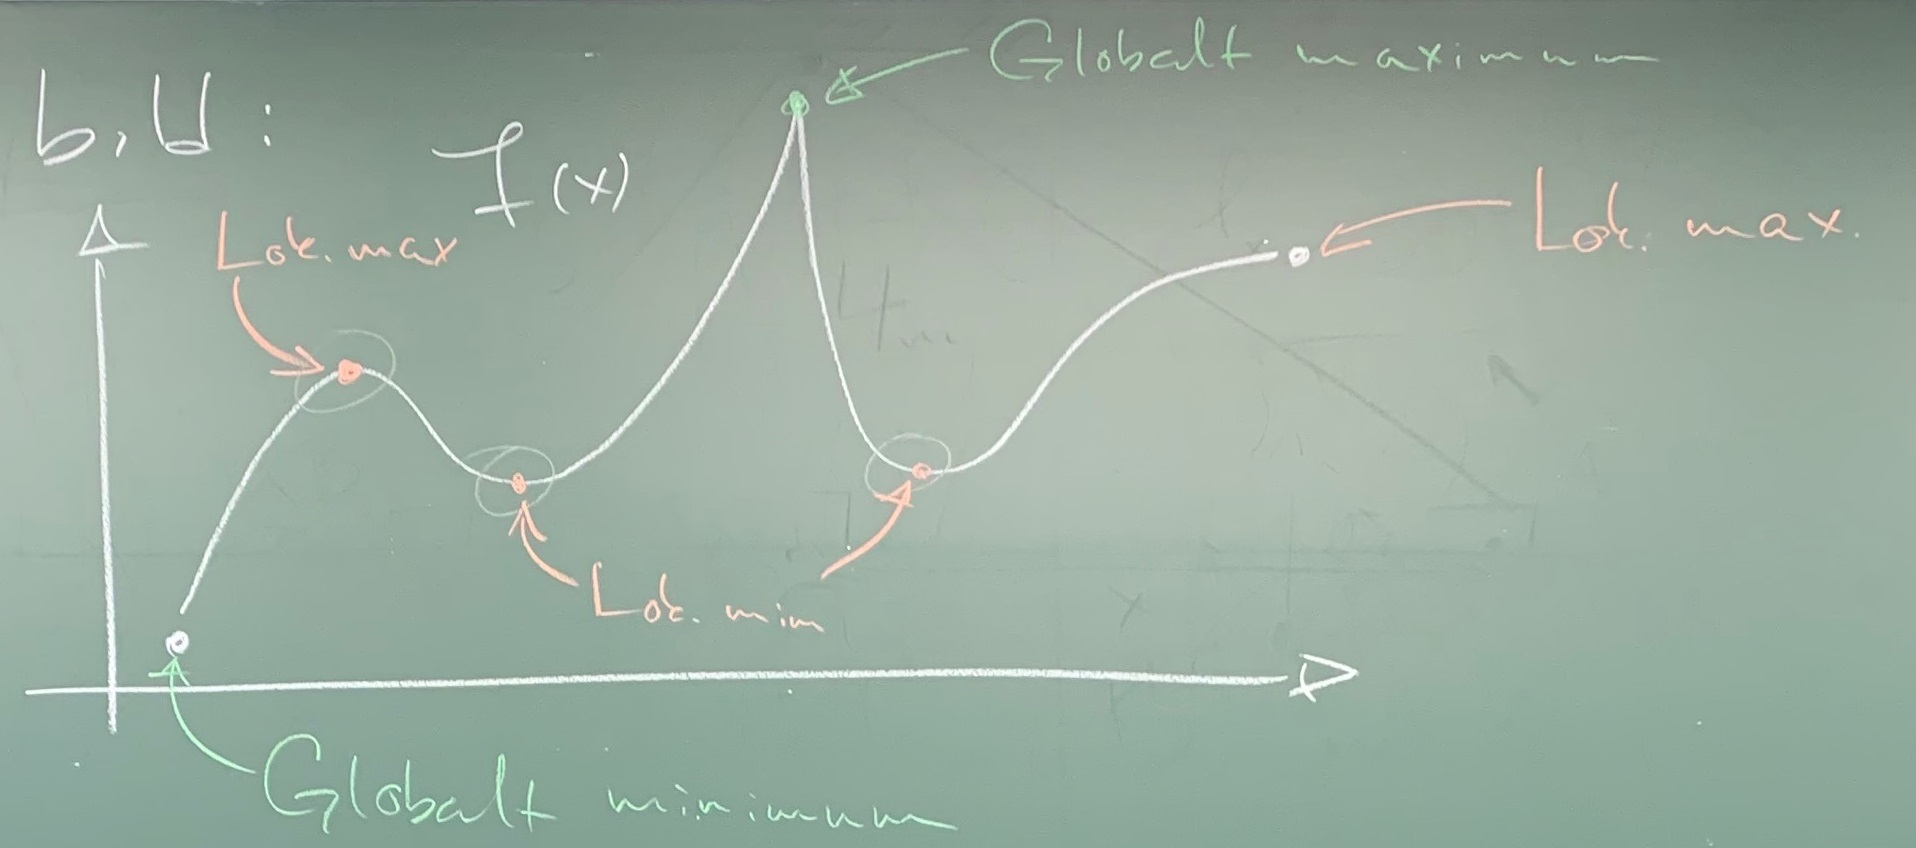
\includegraphics[sacle=0.1]{lessons/lesson10/imgs/img04.jpg}\\
Lokala (och globala) extrempunkter kan hittas i tre olika typer av fall:
\begin{enumerate}
    \item Kritiska punkter, dvs. i $x$ sådana att $f^\prime(x)=0$.
    \item Singulär punkter, dvs i $x$ sådana att $f^\prime(x)$ ej existerar.
    \item Ändpunkter av $D(f)$
\end{enumerate}

\paragraph{Ex (4.4.13)} Hitta alla globala och lokala extrempunkter till $f(x)= |x-1|$, $x\in[-2,2]$
\subparagraph{Lösning} $f$ saknar kritiska punkter (eftersom $f^\prime(x)=sgn(x-1)$).
Har singulär punkt i $x=1$ där $f(1)=0$ och i ändpunkterna gäller att:
\begin{itemize}
    \item $f(-2)= | -2-1| = | -3|=3$
    \item $f(2)= | 2-1| = |1| = 1$
\end{itemize}
så globalt minimum i $x=1$, globalt maximum i $x=-2$ och lokalt maximum i $x=2$.
%infoga bild 5
%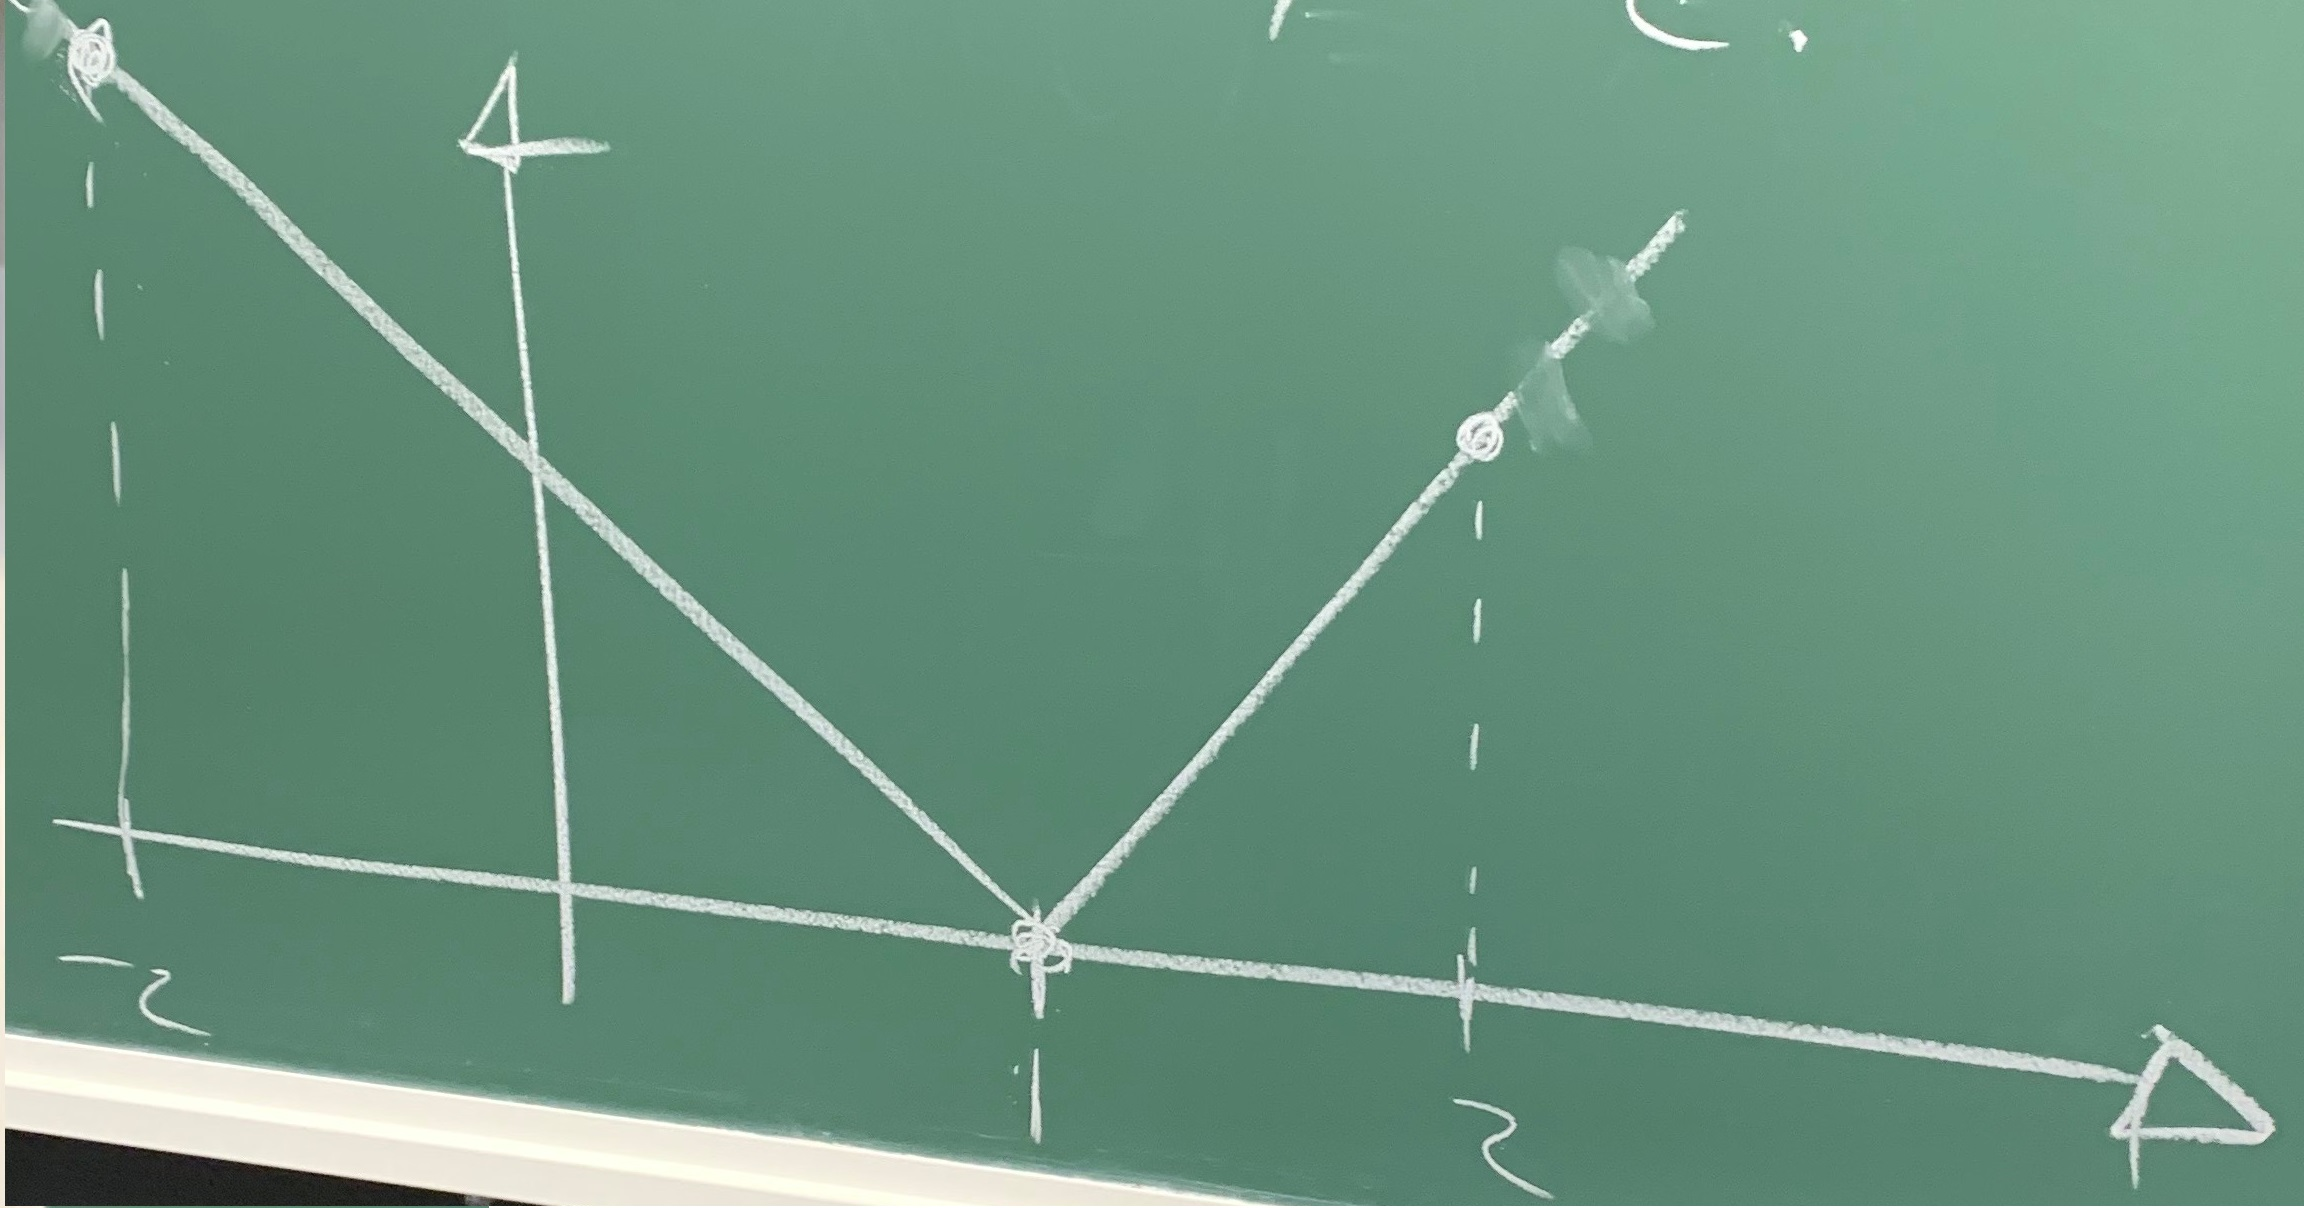
\includegraphics[scale=0.1]{lessons/lesson10/imgs/img05.jpg}\\

%\chapter{Linjär approximation och Taylorutveckling}
Det är vanligt att funktioner modellerar de globala egenskaperna av olika system när teori för tillämpningar utvecklas.
Detta leder ofta till hög komplexitet.
Ibland är man dock bara intresserad av hur systemet beter sig av en viss punkt, säg $x=a$.
Vi kan då använda oss av linjär approximation för att underlätta beräkningar.
Vi vet att den linjära approximationen av $f$ i $x=a$, alltså tangentlinjen, går igenom punkten $(a,f(a))$ och har lutning $f'(a)$.
Detta innebär att $\frac{y-f(a)}{x-a}=f'(a)\Leftrightarrow y=f(a)+f'(a)\cdot (x-a)$.
Alltså, givet en deriverbar funktion $f$ så gäller för $x$-värden "nära" $a$ att $f(x)\approx L(x)=f(a)+f'(a)\cdot (x-a)$.
Hur stort fel innebär denna approximation?
Vi behöver den generaliserande medelvärdessatsen för derivator för att besvara detta.

\paragraph{Sats}
Om $f$ och $g$ är kontinuerliga på $[a,b]$, deriverbar på $(a,b)$ samt att $g'(x)\neq 0$ i $(a,b)$ så finns ett tal så att $\frac{f(b)-f(a)}{g(b)-g(a)}=\frac{f'(c)}{g'(c)}$.

Felet av att approximationen $f(b)$ genom linjen approx $L$ i $x=a$ ges av:
$$E=f(b)-L(b)=f(f)-f(a)-f'(a)\cdot (b-a)$$
Tänk på $E$ som en funktion av $b$ och notera att $E(a)=0$ (dvs $b=a$).
Använd den genom medelvärdessatsen för $E(b)$ och $(b-a)^2$ genom kvoten:
$$\frac{E(b)}{(b-a)^2}=\{E(a)=0\}=\frac{E(b)-E(a)}{(b-a)^2-(a-a)^2} \Rightarrow E(b)=\frac{f''(s)}{2}\cdot (b-a)^2$$
Alltså, felet i att approximera $f(x)$ med $L(x)$ kan beräknas som $E(x)=\frac{f''(x)}{2}(x-a)^2$ för något tal $s$ mellan $a$ och $x$ ($a<s<x$ eller $x<s<a$).
\paragraph{Ex 4.9.12} En kub har sidlängden 20cm.
Ungefär hur mycket måste denna minska om volymen ska minska med 12 cm$^3$?\\
\textbf{Lösning:} Vi vet att $x=20$ cm och vill att $\Delta V=-12$ cm$^3$.
Vi använder linjär approximation av $V$ kring $x=20$ cm.
$L(x)=V(20)+V'(20)\cdot(x+20)$, $\Delta V = V(20)-L(x)=V'(20)\cdot(x-20)=V'(20)\cdot\Delta x$. (\dots)
Kubens sidlängd ska alltså minska ed cirka $1/100=0.01$ cm.

Går det att approximera en funktion $f$ i omgivningen av en punkt $x=a$ på ett bättre sätt än linjärisering?
Vilka egenskaper hos linjäriseringen $L(x)$ gör den till en bra approximation?
$L(x)=f(a)+f'(a)\cdot(x-a)\Rightarrow L(a)=f(a)$ och $L'(a)=f'(a)$.
Kan man hitta en approximation där även andraderivatan stämmer? Ja!
$P(x)=f(a)+f'(a)\cdot(x-a)+\frac{f''(a)}{2}(x-a)^2\Rightarrow P(a)=f(a)$, $P(a)=f'(a)$\\
$P''(a)=0+0+\frac{f''(a)}{2}\cdot 2=f''(a)$
På liknande sätt kan man fortsätta att bygga på med högre ordningens termer.
Det gäller att $\frac{d^n}{dx^n}[(x-a)^n]=\{$kedjeregeln$\}=n\cdot\frac{d^{n-1}}{dx^{n-1}}[(x-a)^{n-a}]=\dots=3\cdot 2\cdot 1$.
Talet $n\cdot (n-1)\cdot\dots\cdot 2\cdot 1$ för $n\in\mathbb{N}$ kallas för $n$-fakultet och skrivs enklare som $n!$.
Man definierar $0!=1$.
Detta gör att man enkelt hittar en approximation $P_n$ till $f$ nära vilken punkt $x=a$ som helst (givet att $f$ är $n$ gånger deriverbar där)
där alla derivator upp till ordning $n$ överensstämmer som $P_n(x)=f(a)+f'(a)\cdot(x-a)+\frac{f''(a)}{2}(x-a)^2+\dots +\frac{f^{(n)}}{n!}(x-a)^n$.
(=$\sum^n_{i=0}\frac{f^{(i)}(a)}{i!}\cdot(x-a)^i$).
Approximation $P_n$ kallas för Taylorpolynomet av grad $n$ runt punkten $x=a$ (eller $n$:te gradens Taylorutveckling).
I specialfallet då $a=0$ kallar man ibland Taylorutvecklingen för Maclaurinutveckling.
Högre ordningens Taylorutvecklingar innebär bättre ock bättre approximationer av $f$ runt $x=a$ som också funkar längre och längre från $x=a$.
Givet $n$:te gradens Taylorpolynom runt $x=a$, alltså $P(x)$, hur bra är approximationen $P(x)\approx f(x)$?
Vi kan visa att feltermer $E_n(x)=\frac{f^{(n+1)}(s)}{(n+1)!}\cdot (x-a)^{n+1}$ för något tal tal $s$ mellan $a$ och $x$.
$E_n(x)$ kallas för Lagranges restterm.

\paragraph{Ex 4.10.10} Använd andra ordningens Taylorpolynom $P_2(x)$ för att approximera $\sqrt{61}$.
Uppskatta även storleken av felet och ge ett intervall där det sanna värdet ligger.\\
%\textbf{Lösning:} Låt $f(x)=\sqrt{}$
\chapter{Linjär approximation och Taylorutveckling}
Det är vanligt att funktioner modellerar de globala egenskaperna av olika system när teori för tillämpningar utvecklas.
Detta leder ofta till hög komplexitet.
Ibland är man dock bara intresserad av hur systemet beter sig av en viss punkt, säg $x=a$.
Vi kan då använda oss av linjär approximation för att underlätta beräkningar.
Vi vet att den linjära approximationen av $f$ i $x=a$, alltså tangentlinjen, går igenom punkten $(a,f(a))$ och har lutning $f'(a)$.
Detta innebär att $\frac{y-f(a)}{x-a}=f'(a)\Leftrightarrow y=f(a)+f'(a)\cdot (x-a)$.
Alltså, givet en deriverbar funktion $f$ så gäller för $x$-värden "nära" $a$ att $f(x)\approx L(x)=f(a)+f'(a)\cdot (x-a)$.
Hur stort fel innebär denna approximation?
Vi behöver den generaliserande medelvärdessatsen för derivator för att besvara detta.

\paragraph{Sats}
Om $f$ och $g$ är kontinuerliga på $[a,b]$, deriverbar på $(a,b)$ samt att $g'(x)\neq 0$ i $(a,b)$ så finns ett tal så att $\frac{f(b)-f(a)}{g(b)-g(a)}=\frac{f'(c)}{g'(c)}$.

Felet av att approximationen $f(b)$ genom linjen approx $L$ i $x=a$ ges av:
$$E=f(b)-L(b)=f(f)-f(a)-f'(a)\cdot (b-a)$$
Tänk på $E$ som en funktion av $b$ och notera att $E(a)=0$ (dvs $b=a$).
Använd den genom medelvärdessatsen för $E(b)$ och $(b-a)^2$ genom kvoten:
$$\frac{E(b)}{(b-a)^2}=\{E(a)=0\}=\frac{E(b)-E(a)}{(b-a)^2-(a-a)^2} \Rightarrow E(b)=\frac{f''(s)}{2}\cdot (b-a)^2$$
Alltså, felet i att approximera $f(x)$ med $L(x)$ kan beräknas som $E(x)=\frac{f''(x)}{2}(x-a)^2$ för något tal $s$ mellan $a$ och $x$ ($a<s<x$ eller $x<s<a$).
\paragraph{Ex 4.9.12} En kub har sidlängden 20cm.
Ungefär hur mycket måste denna minska om volymen ska minska med 12 cm$^3$?\\
\textbf{Lösning:} Vi vet att $x=20$ cm och vill att $\Delta V=-12$ cm$^3$.
Vi använder linjär approximation av $V$ kring $x=20$ cm.
$L(x)=V(20)+V'(20)\cdot(x+20)$, $\Delta V = V(20)-L(x)=V'(20)\cdot(x-20)=V'(20)\cdot\Delta x$. (\dots)
Kubens sidlängd ska alltså minska ed cirka $1/100=0.01$ cm.

Går det att approximera en funktion $f$ i omgivningen av en punkt $x=a$ på ett bättre sätt än linjärisering?
Vilka egenskaper hos linjäriseringen $L(x)$ gör den till en bra approximation?
$L(x)=f(a)+f'(a)\cdot(x-a)\Rightarrow L(a)=f(a)$ och $L'(a)=f'(a)$.
Kan man hitta en approximation där även andraderivatan stämmer? Ja!
$P(x)=f(a)+f'(a)\cdot(x-a)+\frac{f''(a)}{2}(x-a)^2\Rightarrow P(a)=f(a)$, $P(a)=f'(a)$\\
$P''(a)=0+0+\frac{f''(a)}{2}\cdot 2=f''(a)$
På liknande sätt kan man fortsätta att bygga på med högre ordningens termer.
Det gäller att $\frac{d^n}{dx^n}[(x-a)^n]=\{$kedjeregeln$\}=n\cdot\frac{d^{n-1}}{dx^{n-1}}[(x-a)^{n-a}]=\dots=3\cdot 2\cdot 1$.
Talet $n\cdot (n-1)\cdot\dots\cdot 2\cdot 1$ för $n\in\mathbb{N}$ kallas för $n$-fakultet och skrivs enklare som $n!$.
Man definierar $0!=1$.
Detta gör att man enkelt hittar en approximation $P_n$ till $f$ nära vilken punkt $x=a$ som helst (givet att $f$ är $n$ gånger deriverbar där)
där alla derivator upp till ordning $n$ överensstämmer som $P_n(x)=f(a)+f'(a)\cdot(x-a)+\frac{f''(a)}{2}(x-a)^2+\dots +\frac{f^{(n)}}{n!}(x-a)^n$.
(=$\sum^n_{i=0}\frac{f^{(i)}(a)}{i!}\cdot(x-a)^i$).
Approximation $P_n$ kallas för Taylorpolynomet av grad $n$ runt punkten $x=a$ (eller $n$:te gradens Taylorutveckling).
I specialfallet då $a=0$ kallar man ibland Taylorutvecklingen för Maclaurinutveckling.
Högre ordningens Taylorutvecklingar innebär bättre ock bättre approximationer av $f$ runt $x=a$ som också funkar längre och längre från $x=a$.
Givet $n$:te gradens Taylorpolynom runt $x=a$, alltså $P(x)$, hur bra är approximationen $P(x)\approx f(x)$?
Vi kan visa att feltermer $E_n(x)=\frac{f^{(n+1)}(s)}{(n+1)!}\cdot (x-a)^{n+1}$ för något tal tal $s$ mellan $a$ och $x$.
$E_n(x)$ kallas för Lagranges restterm.

\paragraph{Ex 4.10.10} Använd andra ordningens Taylorpolynom $P_2(x)$ för att approximera $\sqrt{61}$.
Uppskatta även storleken av felet och ge ett intervall där det sanna värdet ligger.\\
%\textbf{Lösning:} Låt $f(x)=\sqrt{}$
Givet en funktion $f$ och en punkt $x=a$,
där $f$ är tillräckligt många gånger deriverbar, lärde vi oss att:
\begin{equation*}
    f(x)=p_n(x)+E_n(x)=f(a)+f^\prime(a)(x-a)+...+\frac{f^{(n)}(a)}{n!}(x-a)^n+\frac{f^{n+1}(s)}{(n+1)!}(x-a)^{n+1}
\end{equation*}
för något tal $s$ mellan $a$ och $x$.
Polynomet $P_n(x)$ approx. funktionen $f$ i närheten av $x=a$.
Ofta är man inte intresserad av det exakta uttrycket för felet $E_n(x)$,
utan bara "hur snabbt det växer" i takt med att $x$ rör sig från $a$.
Smidigt att använda så kallad O-notation (dvs. ordo-notation eller stora O-notation).\\
Man skriver att $f(x)=O(u(x))$ då $x\to a$ om det finns tal $K>0$ och $\delta>0$ sådana att $|f(x)|\leq K\cdot|u(x)|$ då $0< |x-a| <\delta$.
På liknande sätt, om $f(x)=g(x)+O(u(x))$ då $x\to a$ så betyder det att $f(x)-g(x)=O(u(x))$.
För Taylor-utv. gäller alltså att $f(x)=P_n(x)+O((x-a)^{n+1})$.\\
Några räkneregler för O:
\begin{itemize}
    \item $C\cdot O(u(x))=O(u(x)),\forall C>0$
    \item $O(f(x))\cdot O(g(x))=O(f(x)\cdot g(x))$
    \item $O(x^m)+O(x^n)=O(x^n)$ om $n\geq m$ och $x\to\infty$
    \item $O(x^m)+O(x^n)=O(x^m)$ om $n\geq m$ och $x\to 0$
    \item Om $f(x)=O((x-a)^k\cdot u(x))$ då $x\to a$ så är $\frac{f(x)}{(x-a)^k}=O(u(x))$ då $x\to a$.
\end{itemize}

\paragraph{Sats (Om taylor-polynom och O)}
Om $f(x)=Q_n(x+O((x-a)^{n+1}))$ då $x\to a$ och $Q_n$ är ett polynom av grad $n$ så är $Q_n=$Taylorpolynomet av $f$ runt $x=a$.
\\\\
Kan förstå l'hopitals regel bättre med hjälp av taylor-polynom och O-notation!
Vi har lärt oss att om gränsvärdet $\lim_{x\to a}\frac{f(x)}{g(x)}$ är av typen $\frac{0}{0}$ och $g^\prime\neq 0$ i en omgivning av $x=a$ så kan man istället föröska beräkna $\lim_{x\to a}\frac{f^\prime(x)}{g^\prime(x)}$.
Om det senare gränsvärdet konvergerar och \underline{inte} är av typen $\frac{0}{0}$ så konvergerar det förra mot samma sak.
\paragraph*{Varför?}~\\
Betrakta första ordningens Taylorutveckling av $f$ och $g$ runt $x=a$:
\begin{equation*}
    f(x)=f(a)+f^\prime(a)\cdot (x-a)+O((x-a)^2)
\end{equation*}
\begin{equation*}
    g(x)=g(a)+g^\prime(a)\cdot (x-a)+O((x-a)^2)
\end{equation*}
\begin{equation*}
    \Rightarrow\lim_{x\to a}\frac{f(x)}{g(x)}=\lim_{x\to a}\frac{f(a)+f^\prime(a)\cdot (x-a)+O((x-a)^2)}{g(a)+g^\prime(a)\cdot (x-a)+O((x-a)^2)}=
\end{equation*}
\begin{equation*}
    =\{f(a)=g(a)=0 \text{ enl. förutsättning}\}=\lim_{x\to a}\frac{f^\prime(a)\cdot (x-a)+O((x-a)^2)}{g^\prime(a)\cdot (x-a)+O((x-a)^2)}=
\end{equation*}
\begin{equation*}
    =\{\text{Bryt ut }(x-a)\text{ ur täljare och nämnare}\}=\lim_{x\to a}\frac{f^\prime(a)+O(x-a)}{g^\prime(a)+O(x-a)}=\frac{f^\prime(a)}{g^\prime(a)}
\end{equation*}
Och om l'Hopital inte funkar, dvs. $\lim_{x\to a}\frac{f^\prime(x)}{g^\prime(x)}$ är av typen $\frac{0}{0}$?
Texta då istället $\lim_{x\to a}\frac{f^{\prime\prime}(x)}{g^{\prime\prime}(x)}$.
Om det gränsvärdet inte är av typen $\frac{0}{0}$ så kommer $\lim_{x\to a}\frac{f(x)}{g(x)}=\lim_{x\to a}\frac{f^{\prime\prime}(x)}{g^{\prime\prime}(x)}$.
\paragraph*{Varför?}~\\
Taylorutveckling till andra ordningen runt $x=a$ ger:
\begin{equation*}
    f(x)=f(a)+f^\prime(a)(x-a)+\frac{f^{\prime\prime}(a)}{2}(x-a)^2+O((x-a)^3)
\end{equation*}
\begin{equation*}
    g(x)=g(a)+g^\prime(a)(x-a)+\frac{g^{\prime\prime}(a)}{2}(x-a)^2+O((x-a)^3)
\end{equation*}
Samma räkning som innan ger att $\lim_{x\to a}\frac{f(x)}{g(x)}=...=\frac{f^{\prime\prime}(a)}{g^{\prime\prime}(a)}$

\paragraph{Ex (kompendie övn. 9.5)} Beräkna gränsvärdet $\lim_{x\to 0}(\frac{1}{sin^2(x)}-\frac{1}{x^2})$
\subparagraph{Lösning} Gränsvärdet är icke-trivialt då direkt insättning av $x=0$ ger $\infty-\infty$.
Börja med lite omskrivningar.
\begin{equation*}
    \frac{1}{sin^2(x)}-\frac{1}{x^2}=\frac{x^2}{x^2sin^2(x)}-\frac{sin^2(x)}{x^2sin^2(x)}=\frac{x^2-sin^2(x)}{x^2sin^2(x)}=
\end{equation*}
\begin{equation*}
    \{cos(2x)=cos^2(x)-sin^2(x)=(1-sin^2(x))-sin^2(x)=1-2sin^2(x)
\end{equation*}
\begin{equation*}
    \text{ så } sin^2(x)=\frac{1-cos^2(x)}{2}\}=\frac{x^2-\frac{1-cos(2x)}{2}}{x^2\frac{1-cos(2x)}{2}}=\frac{2x^2-1+cos(2x)}{x^2-x^2cos(2x)}
\end{equation*}
Från standardutvecklingar vet vi att
\begin{equation*}
    cos(x)=1-\frac{x^2}{2!}+\frac{x^4}{4!}-\frac{x^6}{6!}+...+O(x^{2n+2})
\end{equation*}
\begin{equation*}
    \Rightarrow cos(2x)=1-\frac{(2x)^2}{2!}+\frac{(2x)^4}{4!}-...
\end{equation*}
Använd denna utveckling till ordning 4 i täljaren och ordning 2 i nämnaren!
\begin{equation*}
    \lim_{x\to 0}(\frac{1}{sin^2(x)}-\frac{1}{x^2})=\lim_{x\to 0}\frac{2x^2-1+cos(2x)}{x^2-x^2cos(2x)}=
\end{equation*}
\begin{equation*}
    \lim_{x\to 0}\frac{2x^2-1+(1-\frac{(2x)^2}{2!}+\frac{(2x)^4}{4!}+O(x^6))}{x^2-x^2(1-\frac{(2x)^2}{2!}+O(x^4)}=\lim_{x\to 0}\frac{2x^2-1+1-2x^2+\frac{2}{3}x^4+O(x^6)}{x^2-x^2+2x^4+O(x^6)}=
\end{equation*}
\begin{equation*}
    \lim_{x\to 0}\frac{\frac{2}{3}x^4+O(x^6)}{2x^4+O(x^6)}=\lim_{x\to 0}\frac{x^4}{x^4}\cdot\frac{\frac{2}{3}+O(x^2)}{2+O(x^2)}=\frac{\frac{2}{3}}{2}=\frac{1}{3} \text{ }\Box
\end{equation*}

\paragraph{Ex} Använd Maclaurinutveckling för $sin(x)$ för att beräkna Maclaurinpolynomet av ordning 4 till funktionen $arcsin(x)$.
\begin{equation*}
    sin(x)=x-\frac{x^3}{3!}+\frac{x^5}{5!}-\frac{x^7}{7!}+...+O(x^{2n+1})
\end{equation*}
\subparagraph{Lösning}
Eftersom att $arcsin$ är invers funktion till $sin$ (på intervallet $-\frac{\pi}{2}\leq x \leq \frac{\pi}{2}$) så gäller per definition att:
$arcsin(sin(x))=sin(arcsin(x))=x$ och $arcsin(-sin(x))=arcsin(sin(-x))=-x=\{arcsin(sin(x))=x\}=-arcsin(sin(x))$ så $arcsin(-sin(x))=arcsin(sin(x))=\{sin(x)=z\}$
dvs. $arcsin(-z)=arcsin(z)$.
Detta betyder att $arcsin$ är en udda funktion och utvecklingen vi söker måste därför vara på formeln $a_1x+a_3x^3+O(x^5)$ för några tal $a_1$ och $a_3$.
Vi vet att $sin(arcsin(x))=x$ eftersom (åter igen) $arcsin$ är invers till $sin$,
och vi vet att $sin(x)=x-\frac{x^3}{3!}+O(x^5)$ vilket leder till att
\begin{equation*}
    x=sin(arcsin(x))=(a_1x+a_3x^3+O(x^5))-\frac{(a_1x+a_3x^3+O(x^5))}{6}+O((a_1+a_3x^3+O(x^5))^5)
\end{equation*}
\begin{equation*}
    =(a_1x+a_3x^3+O(x^5))-(\frac{a_1^3}{6}x^3+O(x^5))+O(x^5)=a_1x+(a_3-\frac{a_1^3}{6})x^3+O(x^5)
\end{equation*}
Vilket bara kan vara sant om $a_1=1$ och $a_3-\frac{a_1^3}{6}=0\Rightarrow a_3=\frac{1}{6}$ och vi får att $\arcsin(x)=x+\frac{x^3}{6}+O(x^5)\Box$
\chapter{Summationsnotation}
En summa av tal $a_1+a_2+...+a_n$ skrivs smidigare med summationsnotation:
\begin{equation*}
    a_1+a_2+...+a_n=\sum^n_{i=1} a_i
\end{equation*}
Indexet $i$ kallas för \underline{summationsindex} och existerar bara i själva summationen.
Summering är en linjär operation, dvs superpositionsprincipen gäller:
\begin{equation*}
    \sum_{i=1}^n(\alpha\cdot a_i+\beta\cdot b_i)=\alpha\sum_{i=1}^n a_i + \beta\sum_{i=1}^n b_1
\end{equation*}

Några viktiga standard summor är:
\begin{itemize}
    \item $\begin{matrix}
                  \sum_{i=1}^n 1= & \underbrace{1+1+...+1} & =n \\
                                  & n\text{ ggr}           &
              \end{matrix}$
    \item $\sum_{i=1}^n i=1+2+3+...+n=\frac{n\cdot(n+1)}{2}\text{ (aritmetisk)}$
    \item $\sum_{i=1}^n i^2=1^2+2^2+3^2+...+n^2=\frac{n(n+1)(2n+1)}{6}$
    \item $\sum_{i=1}^n r^{i-1}=1+r+r^2+...+r^{n-1}=\frac{r^n -1}{r-1},r\neq 1 \text{ (geometriskt)}$
\end{itemize}

Vill kunna beräkna arean under funktionsgrafer.
Strategin är att dela upp ytan i mindre bitar för vilka arean är lätt att beräkna och sedan summera alla bidrag.\\
%infoga bild 1
%\includegraphics[scale=0.1]{lessons/lesson14/imgs/img01.jpg}
Dela upp intervallet $[a,b]$ i mindre delintervall med ändpunkter i $a=x_0<x_1<x_2<...<x_n=b$.
Varje delintervall är av bredden $\Delta x=x_1-x_0,\Delta x_2=x_2-x_1,$ osv.
Beräkna (t.ex) areorna av alla rektanglar med bred $\Delta x_i$ och höjd $\frac{f(x_i)+f(x_i+1)}{2}$ (medelvärdet).
Då borde $A\approx \sum_{i=0}^{n-1}\frac{f(x_1)+f(x_{i+1})}{2}\cdot\Delta x_i=\sum_{i=0}^{n-1} A_i$.
Approximationen \underline{borde} bli bättre och bättre i takt med att delintervallen blir mindre och mindre och det borde gälla att
\begin{equation*}
    A=\begin{matrix}
        lim        \\
        n\to\infty \\
        \Delta x_i\to 0
    \end{matrix}\sum_{i=0}^{n-1}A_i
\end{equation*}
Detta måste dock preciseras för att bli matematiskt relevant.

\paragraph{Ex (5.2.5)} Beräkna areorna under grafen till $y=x^2$ mellan $x=1$ och $x=3$.
\subparagraph*{Lösning}
%infoga bild 2
%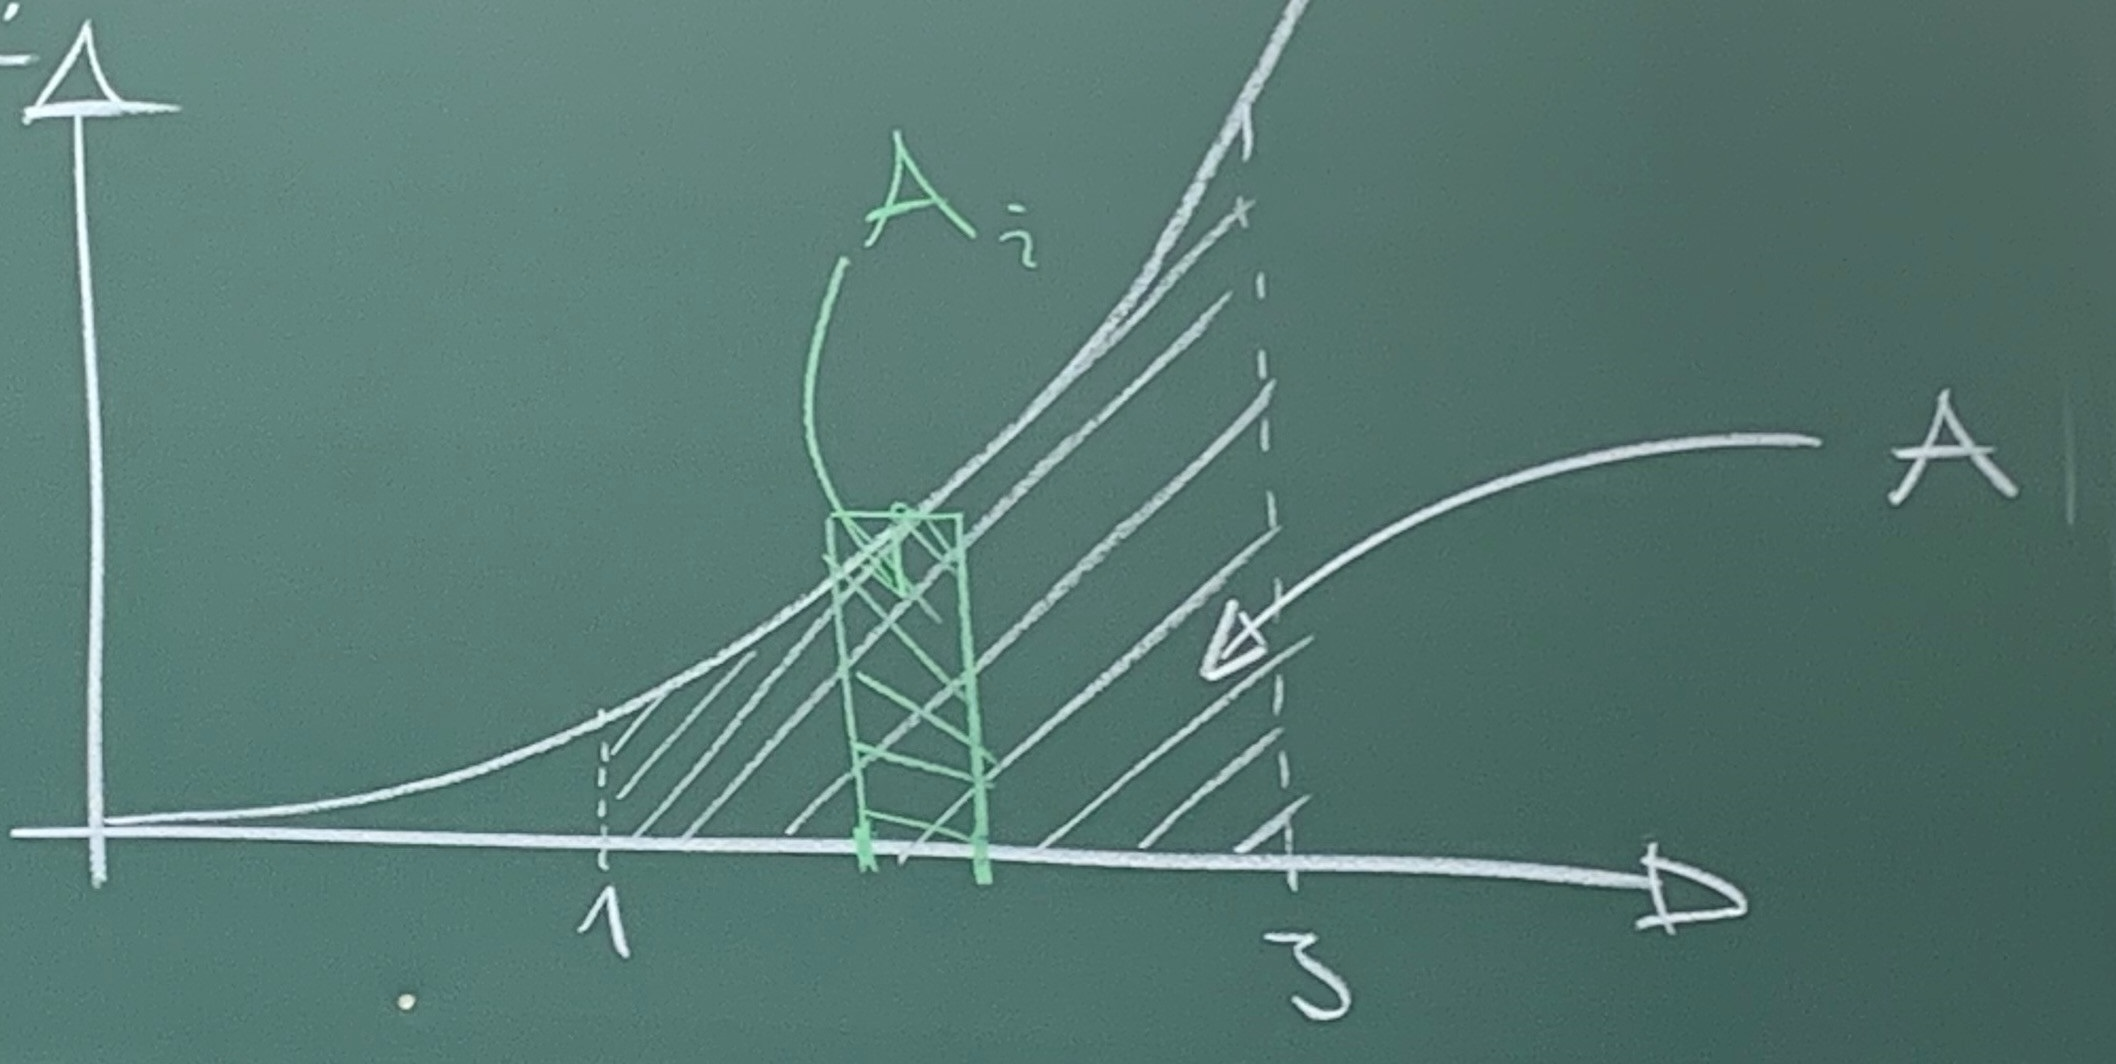
\includegraphics[scale=0.1]{lessons/lesson14/imgs/img02.jpg}
Dela upp intervallet $[1,3]$ i $n$ stycken lika stora delar.
Delintervallets bredd blir då $\Delta x=\frac{3-1}{n}=\frac{2}{n}$ med ändpunkter i $1,1+\frac{2}{n},1+2\frac{2}{n},...,1+(n-2)\frac{2}{n},3$.
Om vi använder funktionens medelvärde i varje delintervall som höjd för att approximerande rektanglar får vi att:
\begin{equation*}
    A=\lim_{n\to\infty}\sum_{i=1}^n \frac{f(x_i)+f(x_{i-1})}{2}\cdot\delta x=
    \lim_{n\to\infty}\sum_{i=1}^n \frac{(1+i\cdot\frac{2}{n})^2+(1+(i-1)\frac{2}{n})^2}{2}\cdot\frac{2}{n}=
\end{equation*}
\begin{equation*}
    \lim_{n\to\infty}\sum_{i=1}^n\frac{1+\frac{4i}{n^2}+\frac{4i^2}{n^2}+1+\frac{4i}{n}-\frac{4}{n}+\frac{4i^2}{n^2}-\frac{8i}{n^2}+\frac{4}{n^2}}{2}\frac{2}{n}=
    \lim_{n\to\infty}\sum_{i=1}^n\frac{2}{n}+\frac{8i}{n^2}+\frac{8i^2}{n^3}-\frac{4}{n^2}-\frac{8i}{n^3}+\frac{4}{n^3}=
\end{equation*}
\begin{equation*}
    \lim_{n\to\infty}(\frac{2}{n}\cdot n+\frac{8}{n^2}\cdot\frac{n(n+1)}{2}+\frac{8}{3}\cdot\frac{n(n+1)(2n+1)}{6}-\frac{4}{n^2}\cdot n-\frac{8}{n^3}\cdot\frac{n(n+1)}{n}+\frac{4}{n^3}\cdot n=
\end{equation*}
\begin{equation*}
    2+4+\frac{16}{6}=6+\frac{8}{3}=\frac{26}{3}\text{ a.e }\Box
\end{equation*}
~\\
För att areaberäkning genom approx. med staplar ska vara "vettig" mpste det gälla att resultatet är oberoende av:
\begin{enumerate}
    \item hur $x$-axeln styckas upp
    \item vilken stapelhöjd som väljes i varje delintervall (dvs overoende av $f(s)$ där $s\in[x_i,x_{i+1}]$)
\end{enumerate}
En uppdelning av ett intervall $[a,b]$ i disjunkta delintervall $[x_0,x_1],(x_1,x_2],...,(x_{n-1},x_n]$ kallas för en \underline{partition} av $[a,b]$ och kan refereras till som mängden av ändpunkter:
\begin{equation*}
    P=\{x_0,x_1,...,x_n\}
\end{equation*}
Varje delintervall i $P$ har en längd $\Delta x_i=x_{i-1}-x_i$ och man definierar \underline{normen} som längden av det längsta delintervallet:
\begin{equation*}
    ||P||:=\begin{matrix}
        \text{max} \\
        1\leq i \leq n
    \end{matrix}\Delta x_i
\end{equation*}
Om $f$ är en kontinuerlig funktion så antas både ett maximalt och ett minimalt värde någonstans i varje delintervall, säg i $x=u_i$ och $x=l_i$ för delintervallet $[x_i,x_{i+1}]$.
% infoga bild 3
%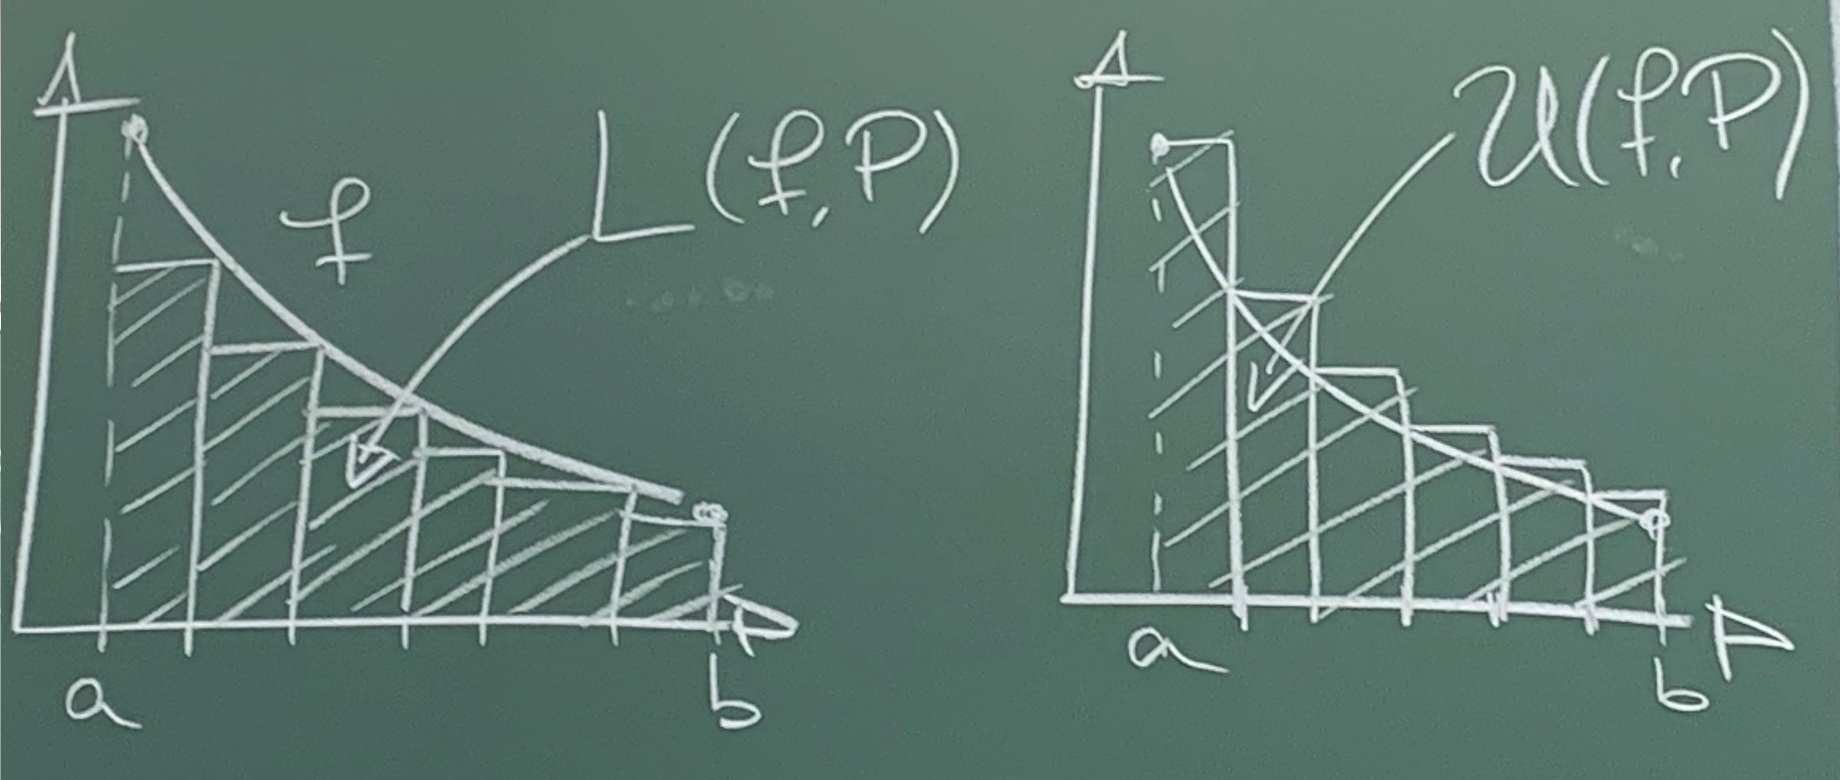
\includegraphics[scale=0.1]{lessons/lesson14/imgs/img03.jpg}
Dvs. om $x\in[x_i,x_{i+1}]$ så gäller att $f(l_i)\leq f(x)\leq f(u_i)$.
Det betyder att en godtycklig stapel över intervallet $[x_i,x_{x+i}]$ \underline{alltid} kommer att ha en area $A_i$ så att
\begin{equation*}
    f(l_i)\cdot\Delta x_i\leq A_i\leq f(u_i)\cdot\Delta x_i
\end{equation*}
Givet en partition $P$ kan vi definiera den nedåt begränsande Riemann-summan $L(f,P)$ och den övre begränsande $U(f,P)$ som:
\begin{equation*}
    L(f,P)=\sum_{i=1}^n f(l_i)\cdot\Delta x
\end{equation*}
\begin{equation*}
    U(f,P)=\sum_{i=1}^n f(u_i)\cdot\Delta x
\end{equation*}
%infoga bild 4
%\includegraphics[scale=0.1]{lessons/lesson14/imgs/img04.jpg}
Om $f$ beter sig "vettigt" och $P$ blir en finare och finare partion av intervallet $[a,b]$ där $||P||\overrightarrow{n\to\infty}0$ så \underline{borde} $\lim_{n\to\infty}L(f,P)=\lim_{n\to\infty}U(f,P)$ oavsett val av partition $P$.
I så fall är det ett rimligt mått av arean under funktionsgrafen.
Detta definierar den \underline{definita intergralen} av $f$ mellan $a$ och $b$.

\paragraph{Definition (definit integral) (tenta)} Antag att det finns precis ett enda tal $I$ så att det för varje partition $P$ av $[a,b]$ gäller att: $L(f,P)\leq I\leq U(f,P)$\\
I så fall säger man att $f$ är \underline{intergrerbar} över $[a,b]$ och vi kallar talet $I$ för den \underline{definita integralen} av $f$ över $[a,b]$.
Detta skrivs symboliskt som
\begin{equation*}
    I=\int_{a}^{b} f(x) \,dx
\end{equation*}
Notera att $\int_{a}^{b} f(x) \,dx$ är ett \underline{tal} och inte en funktion.
"Variabeln" $x$ existerar endast inuti integralen och kallas för \underline{integrationsvariabel}.
Talen $a$ och $b$ kallas nedre- och övre-integransgräns.
Funktionen $f$ kallas för \underline{integrand} och $dx$ för \underline{differntialen}.


Definierade utifrån Riemann-summor är en hörnsten inom matematisk analys tillsammans med definitionen av derivatan och definitionen av gränsvärde.
Räcker gott och väl för praktiska tillämpningar men ej för vidare teoretiskt arbete (då används Lebesque integralen).
\chapter{Definita integraler}
Den efinita integralen $\int_a^b f(x)\, dx$ av en kontinuerlig funktion
$f$ över ett intervall $[a,b]$ definieras som det \underline{unika tal}
$I$ som alltid ligger mellan godtycklig nedåt begränsad- och övrebegränsad Riemannsumma (om det finns):
\begin{equation*}
    L(f,P)\leq I \leq U(f,P)
\end{equation*}
för \underline{alla} tänkbara partitioner $P$ av $[a,b]$.\\
Geometriskt tolkas $\int_a^b f(x)\, dx$ som "arean under grafen till $f$ med tecken".\\
%infoga bild 1
% 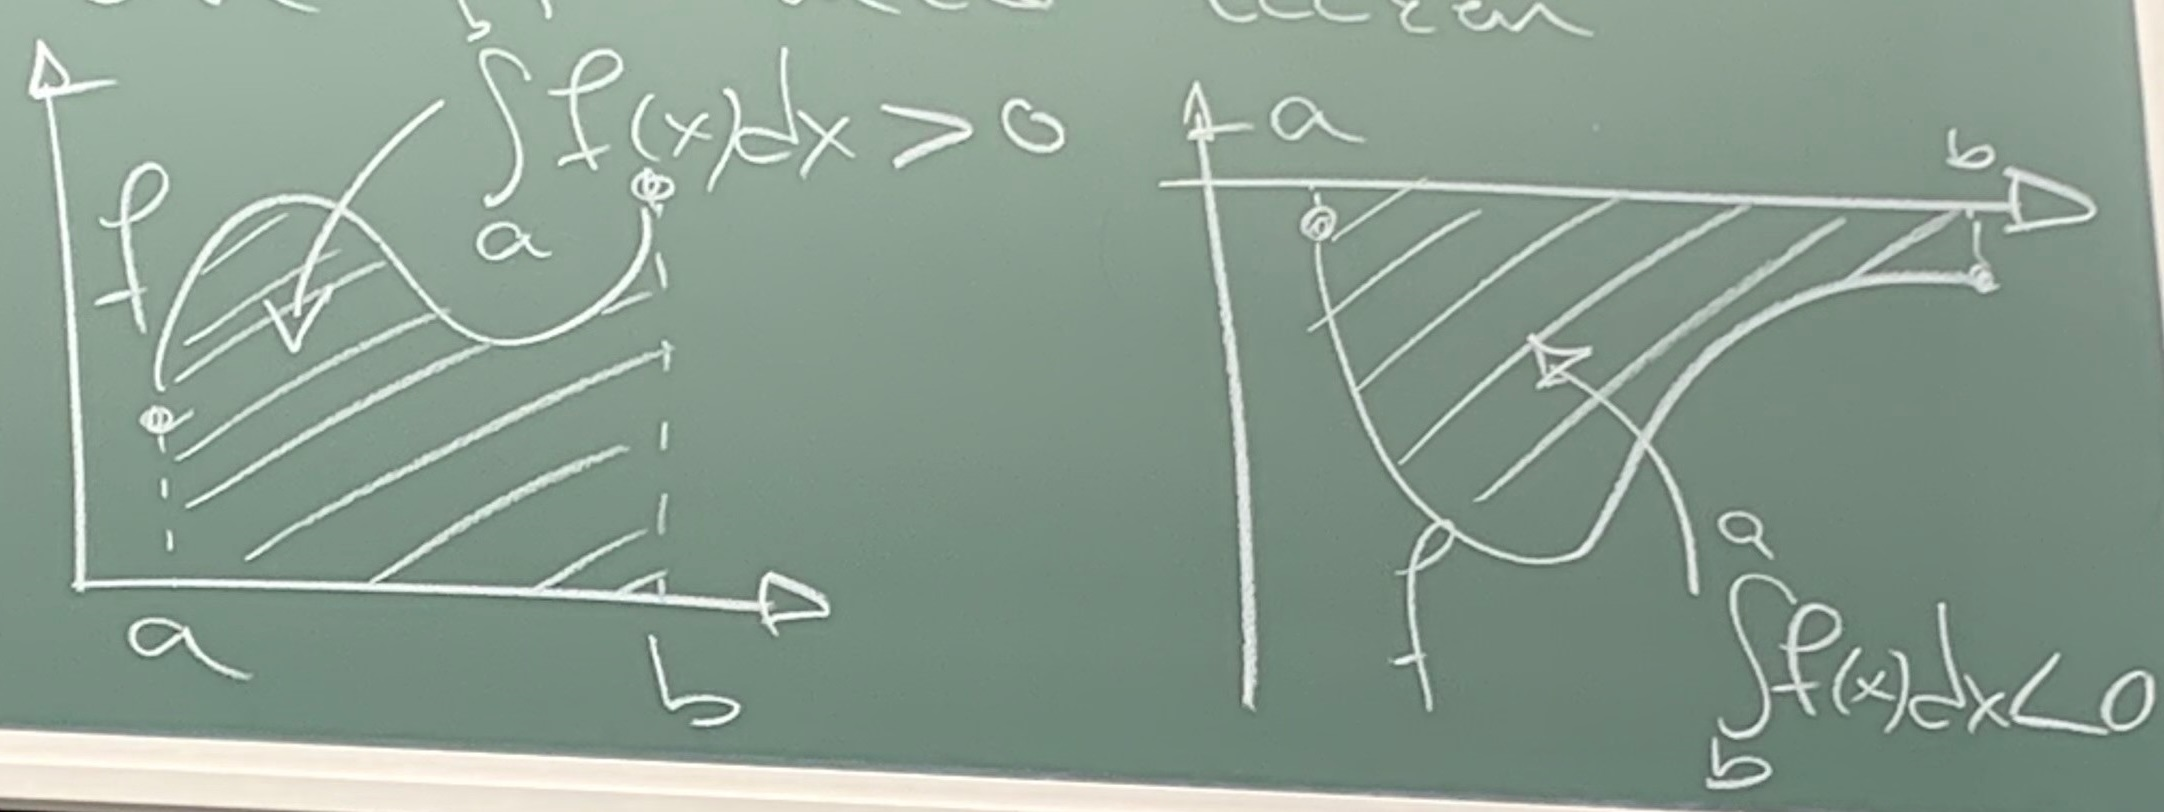
\includegraphics{lessons/lesson15/imgs/img01.jpg}\\

Har här förutsatt att $a<b$, men är naturligt att utvidga konceptet med definit intergral genom följande definitioner:
\begin{itemize}
    \item $a=b\Rightarrow \int_a^b f(x)\, dx = 0$
    \item $a>b\Rightarrow \int_a^b f(x)\, dx = - \int_a^b f(x)\, dx$
\end{itemize}
Integrering är en \underline{linjär} operation, dvs. superpositionsprincipen gäller:
\begin{equation*}
    \int_{a}^{b} \alpha \cdot f(x) +\beta \cdot g(x) \, dx =
    \alpha \int_{a}^{b} f(x)\, dx + \beta \int_{a}^{b} g(x)\, dx
\end{equation*}
för alla $\alpha,\beta\in\mathbb{R}$.
Rent geometriskt gäller också följande:
\begin{itemize}
    % infoga bild 2
    \item $\Rightarrow \int_a^c f(x)\, dx = \int_a^b f(x)\, dx + \int_b^c f(x)\, dx$
          % infoga bild 3
    \item $\Rightarrow \int_a^b f(x)\, dx \leq \int_a^b g(x)\, dx$
          % infoga bild 4
    \item $\Rightarrow |\int_a^b f(x)\, dx| \leq \int_a^b |f(x)|\, dx$ (triangelolikheten)
          %infoga bild 5
    \item $\Rightarrow \int_{a-b}^{a+b} f(x)\, dx = 2\cdot\int_{a-b}^{a} f(x)\, dx = 2\cdot\int_{a}^{a+b} f(x)\, dx$\\
          $f$ \underline{jämn} med avseende på $x=a$
          %infoga bild 6
    \item $\Rightarrow \int_{a-b}^{a+b} f(x)\, dx = 0$\\
          $f$ \underline{udda} med avseende på $x=a$
\end{itemize}

För kontinuerliga funktioner och för derivator gäller "medelvärdessatser".
\begin{itemize}
    \item $f$ kontinuerlig på $[a,b] \Rightarrow$ det finns en punkt $c\in[a,b]$ där $f$ antar värdet $\frac{f(a)-f(b)}{2}$
    \item $f$ deriverbar på $(a,b)\Rightarrow$ det finns en punkt $c\in(a,b)$ där derivatan av $f$ motsvarar snittlutningen på intervallet,
          dvs. $f^\prime(c)=\frac{f(b)-f(a)}{b-a}$
\end{itemize}

Analog medelvärdessats finns också för definita integraler!

\paragraph*{Sats (Medelvärdessatsen för definita integraler)}
Om $f$ är kontinuerlig på $[a,b]$ så finns en punkt $c\in[a,b]$ så att
\begin{equation*}
    \int_a^b f(x)\, dx = (b-a) \cdot f(c)
\end{equation*}
Medelvärdessatsen för integraler säger att det finns en rektangel med bred $b-a$ och höjd $f(c)$ (för något $c\in[a,b]$) vars area är precis $\int_a^b f(x)\, dx$.\\
%infoga bild 7
% 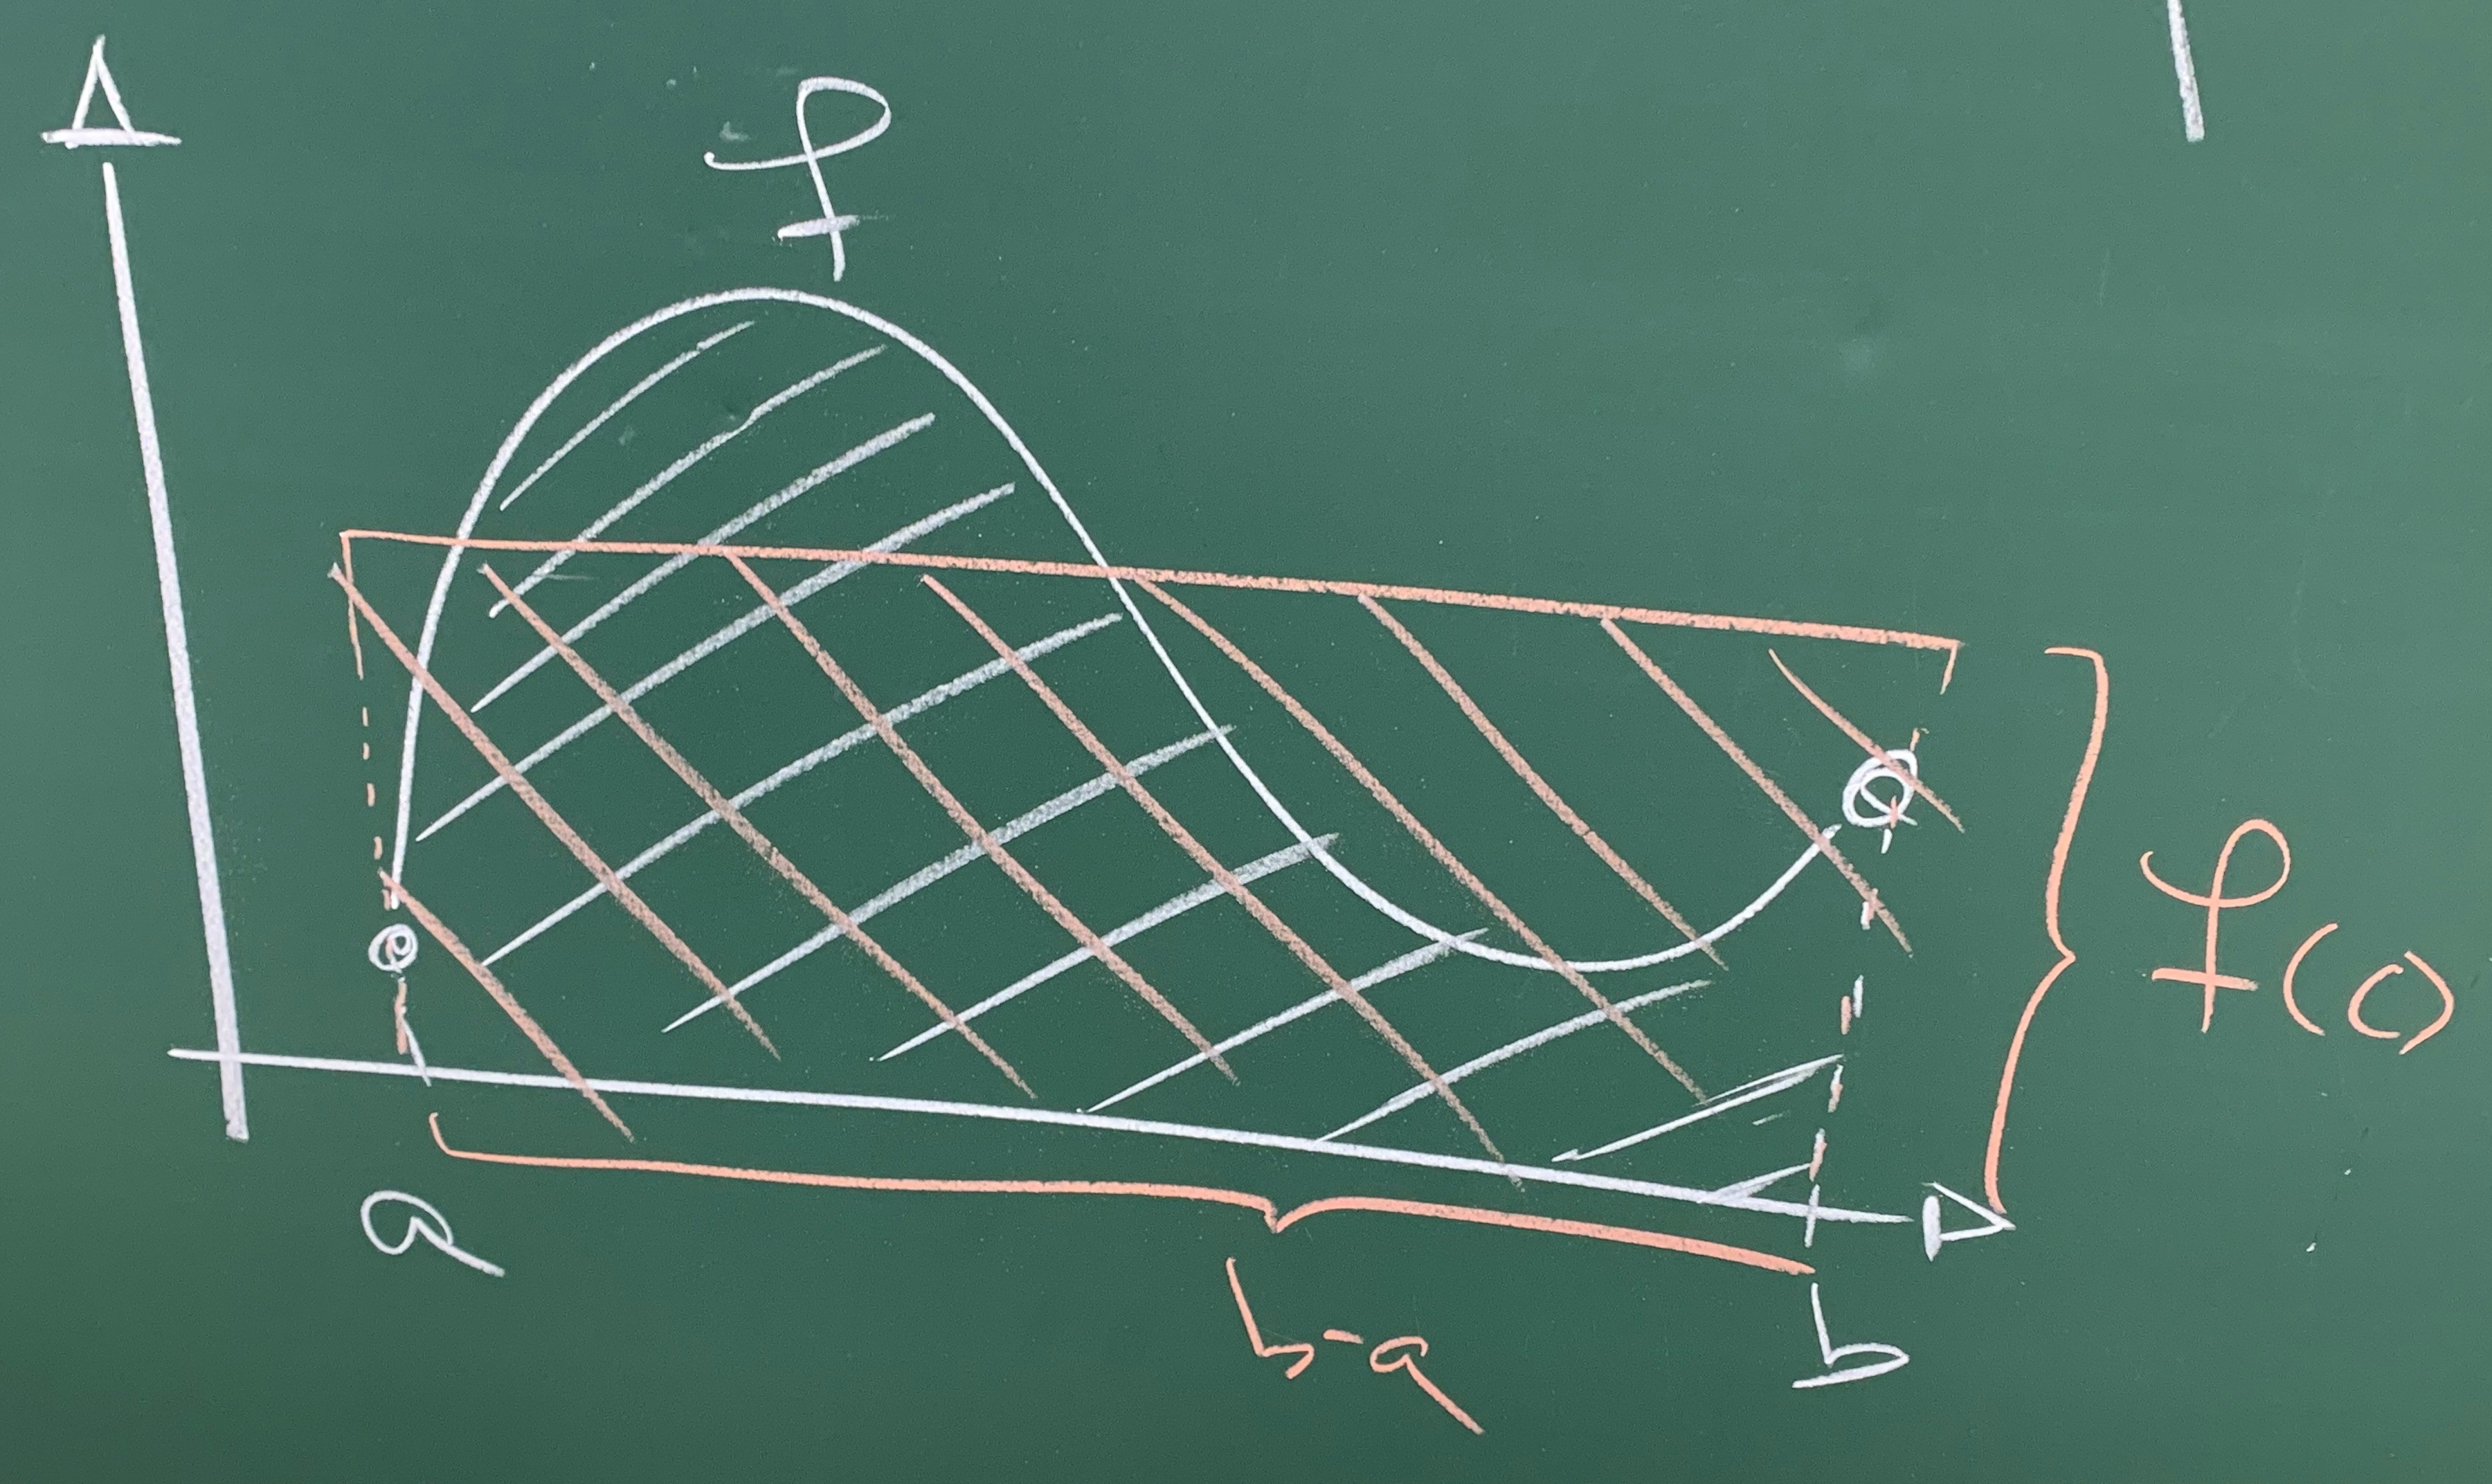
\includegraphics[]{lessons/lesson15/imgs/img07.jpg}\\
Ur detta resultat \underline{definieras} medelvärdet av en funktion $f$ (integrerbar) på ett intervall $[a,b]$ som:
$\overline{f}\frac{1}{b-a}\cdot \int_a^b f(x)\, dx$ (rimligare än t.ex. att sätta medelvärdet som $\frac{f(a)+f(b)}{2}$ eftersom integralen tar hänsyn till $f$ över \underline{hela} intervallet $[a,b]$ och inte bara ändpunkterna).

\chapter{Analysens huvudsats}
Att definiera integraler genom Riemann-summor är bra på många sätt, inte minst för att det är intuitivt, men vi måste ha ett smidigare sätt att beräkna $\int_a^b f(x)\, dx$ (håller ej att behöva beräkna gränsvärdet $L(f,P)$ och $U(f,P)$).
Detta löser delvis analysens huvudsats.

\paragraph*{Sats (Analysen huvudsats) (tenta)}
Antaga att funktionen $f$ är kontinuerlig på ett intervall $I$ som innehåller punkten $a$.
\begin{enumerate}
    \item Låt $F$ vara en funktion på $I$ definierat som $F(x)=\int_a^xf(t)\, dt$
          Då är $F$ deriverbar på $I$ och $F^\prime(x)=f(x)$, dvs.
          \begin{equation*}
              \frac{d}{dx}\int_a^x f(t)\,dt=f(x)
          \end{equation*}
          (så derivering är "antioperationen" till integrering!)
    \item Om $G(x)$ är en primitiv funktion till $f(x)$ på $I$,
          dvs. $G^\prime(x)=f(x)$ så gäller för varje $b\in I$ att:
          \begin{equation*}
              \int_a^b f(x)\,dx=G(b)-G(a)
          \end{equation*}
          (dvs. en beräkningsformel för integraler)
\end{enumerate}
\subparagraph{Bevis}

\begin{enumerate}
    \item Med definitionen av funktionen $F$ enligt satsen gäller att:
          \begin{equation*}
              F^\prime(x)=\lim_{h\to 0}\frac{F(x+h)-F(x)}{h}=
              \lim_{h\to 0}\frac{1}{h}(\int_a^{x+h}f(t)\, dt - \int_a^x f(t)\, dt)=
          \end{equation*}
          \begin{equation*}
              lim_{h\to 0}\frac{1}{h}\in_x^{x+h} f(t)\, dt=
              \{\text{medelvärdessatsen för integraler}\}=
          \end{equation*}
          \begin{equation*}
              \lim_{h\to 0}\frac{1}{h}(x+h-x)\cdot f(c)=
              \lim_{h\to 0}\frac{1}{h}\cdot h\cdot f(c)=\lim_{h\to 0}f(c)
          \end{equation*}
          för något tal $c\in[x,x+h]$.
          Men vi vet att $f$ är kontinuerlig på intervallet $I$ och
          därmed att $\lim_{h\to 0}f(c)=f(x)$ och alltså är
          $F^\prime(x)=f(x)$ dvs. att $\frac{d}{dx}\int_a^xf(t)\, dt= f(x)$ $\Box$
    \item Om $G^\prime = f(x)$ så är $F(x)=G(x)+C$ på $I$ för något tal
          $C\in\mathbb{R}$ (eftersom två olika primitiva funktioner till
          $f$ endast kan skilja på konstanten).
          Alltså gäller att $\int_a^x f(t)\, dt=G(x)+C$ och om $x=a\Rightarrow 0=G(a)-C$ så $C=-G(a)$-
          Om vi nu sätter $x=b$ får vi att $\int_a^b f(x)\, dx=G(b)-G(a)$ $\Box$
\end{enumerate}

\paragraph{Ex (5.5.15)} Beräkna $\int_0^e a^x\, dx$ $a>0$
\subparagraph{Lösning}
För att lösa problemet vill vi hitta en primitiv funktion till $a^x$,
dvs. $\int a^x\, dx$.
Det gäller att $a^x=e^{ln(a^x)}=e^{x\cdot ln(a)}$. Men $\frac{d}{dx}(e^{x\cdot ln(a)})=ln(a)\cdot e^{x\cdot ln(a)}$
så $\int e^{x\cdot ln(a)}\, dx= \frac{1}{ln(a)}\cdot x^{x\cdot ln(a)}=\frac{a^x}{ln(a)}$.
Så enligt analysens huvudsats gäller $\int_0^e a^x\, dx=[\frac{a^x}{ln(a)}]_0^e=\frac{e^e}{ln(a)}-\frac{a^0}{ln(a)}=\frac{1}{ln(a)}\cdot (a^e-1) \Box$
\chapter{Att integrera}
Analysen huvudsats gör det möjligt att beräkna integraler på ett vettigt sätt (utan att konkret jobba med Riemann-summor).
Jan dock vara mycket svårt ändå!

För att lösa olika typer av integrationsproblem behövs:
\begin{enumerate}
    \item Erfarenhet och mycket träning!
    \item En samling metoder och trix.
\end{enumerate}

\section*{Variabelsubstitution}
Grundläggande och viktig metod för att beräkna vissa typer av integraler.
Utgår från kedjeregeln, fast "baklänges":
\begin{equation*}
    \frac{d}{dx}(fg(x))=f^\prime(g(x))\cdot g^\prime(x)\Rightarrow
    \int f^\prime(g(x))\cdot g^\prime(x)\, dx=
    \left\lbrace\begin{matrix}
        u=g(x) \\
        du=g^\prime\, dx
    \end{matrix}\right\rbrace =
\end{equation*}
\begin{equation*}
    \int f^\prime(u)\, dx=
    f(u)+C=\{u=g(x)\}=f(g(x))+C\text{ för } C\in\mathbb{R}
\end{equation*}
Så, om man vill lösa en integral där integranden är på formen $f^\prime(g(x))\cdot g\prime(x)$ för några funktioner $f(x)$ och $g(x)$ (kan vara svåra att identifiera!),
prova att byta variabel från $x$ till $u=g(x)$.

Funkar även för definita integraler:
\begin{equation*}
    \int_a^b f^\prime(g(x))\cdot g^\prime(x)\, dx=
    \left\lbrace\begin{matrix}
        u=g(x)              &  & x=a\Rightarrow u=g(a) \\
        du=g^\prime(x)\, dx &  & x=b\Rightarrow u=g(b)
    \end{matrix}\right\rbrace =
    \int_{g(a)}^{g(b)}f^\prime(u)\, du
\end{equation*}

\paragraph*{Ex (5.6.4)} Lös integralen $\int e^{2x}\cdot \sin(e^{2x})\, dx$.
\subparagraph*{Lösning}
Observera att $\frac{d}{dx}(e^{2x})=2\cdot e^{2x}$ så vi kan skriva
\begin{equation*}
    \int e^{2x}\sin(e^{2x})\, dx=
    \frac{1}{2}\int 2e^{2x}\sin(e^2x)\, dx
\end{equation*}
Använd Variabelsubstitution med $f(x)=sin(x)$ och $g(x)=e^{2x}$.
\begin{equation*}
    \frac{1}{2}\int sin(e^{2x})\cdot 2e^{2x}\, dx=
    \begin{bmatrix}
        u=e^{2x} \\
        du=2e^{2x}\, dx
    \end{bmatrix}=
    \frac{1}{2}\int \sin(u)\, du=
\end{equation*}
\begin{equation*}
    \frac{1}{2}(-cos(u))+C=
    C-\frac{1}{2}cos(e^{2x}), C\in\mathbb{R}
\end{equation*}

\paragraph*{Ex (5.6.41)} Beräkna integralen $\int_0^{\frac{\pi}{2}}\sin^4(x)\, dx$.
\subparagraph{Lösning}
Inte uppenbart på förhand.
Krävs erfarenhet och trigonometri:
\begin{equation*}
    \int_0^{\frac{\pi}{2}}\sin^4(x)\, dx=
    \int_0^{\frac{\pi}{2}}(sin^2(x))^2\, dx=
\end{equation*}
\begin{equation*}
    \{\cos 2x=1-2\sin^2(x)\Leftrightarrow sin^2(x)=\frac{1-cos(2x)}{2}\}=
    \int_0^{\frac{\pi}{2}}(\frac{1-cos(2x)}{2})^2\, dx=
\end{equation*}
\begin{equation*}
    \frac{1}{4}\int_0^{\frac{\pi}{2}}1-2\cos(2x)+cos^2(2x)\, dx=
\end{equation*}
\begin{equation*}
    \frac{1}{4}\int_0^{\frac{\pi}{2}}\, dx-\frac{2}{4}\int_0^{\frac{\pi}{2}}cos(2x)\, dx+\frac{1}{4}\int_0^{\frac{\pi}{2}}cos^2(2x)\, dx=
\end{equation*}
\begin{equation*}
    \{cos(4x)=2cos^2(2x)-1\Leftrightarrow cos^2(2x)=\frac{cos(4x)+1}{2}\}=
\end{equation*}
\begin{equation*}
    \frac{1}{4}[x]_0^{\frac{\pi}{2}}-\frac{1}{2}[\frac{1}{2}\sin(2x)]_0^\frac{\pi}{2}+\frac{1}{8}\int_0^\frac{\pi}{2}\cos(4x)+1\, dx=
\end{equation*}
\begin{equation*}
    \frac{\pi}{8}+\frac{1}{8}(\frac{1}{4}\sin(2\pi)+\frac{\pi}{2}-\frac{1}{4}\sin(0)-0)=
    \frac{\pi}{8}+\frac{\pi}{16}=
    \frac{2\pi}{16}+\frac{\pi}{16}=
    \frac{3\pi}{16}
\end{equation*}
Formlerna för "dubbla vinkeln" är väldigt ofta användbara om integranden involverar \underline{jämna potenser} av $\sin(x)$ och $\cos(x)$!

\section{Partiell integration}
En mycket användbar metod för att lösa integraler som fås ur produktregeln för derivator:
\begin{equation*}
    \frac{d}{dx}(f(x)\cdot g(x))=f^\prime(x)\cdot g(x)+f(x)\cdot g^\prime(x)
\end{equation*}

Om $F(x)$ är en primitiv funktion till $f(x)$ så kan vi stället skriva:
\begin{equation*}
    \frac{d}{dx}(F(x)\cdot g(x))=F^\prime(x)\cdot g(x)+F(x)\cdot g^\prime(x)=
    \{F^\prime(x)=f(x)\}=f(x)\cdot g(x)+F(x)\cdot g^\prime(x)
\end{equation*}
Omskrivet får vi:
\begin{equation*}
    f(x)\cdot g(x)=\frac{d}{dx}(F(x)\cdot g(x))-F(x)\cdot g^\prime(x)
\end{equation*}
\begin{equation*}
    \text{Med def. intervall } \int_a^b f(x)\cdot g(x)=[F(x)\cdot g(x)]_a^b-\int_a^b F(x)\cdot g^\prime(x)\, dx
\end{equation*}
och om vi integrerar båda sidor och använder analysens huvudsats finner man att:
\begin{equation*}
    \int f(x)\cdot g(x) = \int\frac{d}{dx}(F(x)\cdot g(x))\, dx - \int F(x)\cdot g^\prime(x)\, dx=
    F(x)\cdot g(x)-\int F(x)\cdot g^\prime(x)\, dx
\end{equation*}

Detta samband kallas för \underline{partiell integration}.
Användbart när integralen $\int F(x)\cdot g^\prime(x)\, dx$ är lättare än $\int f(x)\cdot g(x)\, dx$.

\paragraph*{Ex (6.1.6)} Lös integralen $x(ln(x))^3\, dx$.
\subparagraph{Lösning}
Använd partiell integration med $f(x)=x$ och $g(x)=(ln(x))^3$.
\begin{equation*}
    \Rightarrow\int x(ln(x))^3\, dx=
    \frac{x^2}{2}(\ln(x))^3-\int \frac{x^2}{2}\cdot 3(\ln(x))^2\frac{1}{x}\, dx=
\end{equation*}
\begin{equation*}
    \frac{x^2}{2}(\ln(x))^3-\frac{3}{2}\int x(\ln(x))^2\, dx=
    \{\text{part. int.}\}=
\end{equation*}
\begin{equation*}
    \frac{x^2}{2}(\ln(x))^3-\frac{3}{2}(\frac{x^2}{2}(\ln(x))^2-\int \frac{x^2}{2}\cdot 2(\ln(x))\frac{1}{x}\, dx)=
\end{equation*}
\begin{equation*}
    \frac{x^2}{2}(\ln(x))^3-\frac{3}{4}x^2(\ln(x))^2+\frac{3}{2}\int x\ln(x)\, dx=
    \{\text{parti. int.}\}=
\end{equation*}
\begin{equation*}
    \frac{x^2}{2}(\ln(x))^3-\frac{3}{4}x^2(\ln(x))^2+\frac{3}{2}(\frac{x^2}{2}\ln(x)-\int \frac{x^2}{2}\cdot\frac{1}{x}\, dx)-\frac{3}{4}\int x\, dx=
\end{equation*}
\begin{equation*}
    \frac{x^2}{2}(\ln(x))^3-\frac{3}{4}x^2(\ln(x))^2+\frac{3}{4}x^2\ln(x)-\frac{3}{4}\cdot\frac{x^2}{2}+C, C\in\mathbb{R}
\end{equation*}
så $\int x(\ln(x))^3\, dx=\frac{x^2}{2}(\ln(x))^3-\frac{3}{4}x^2(\ln(x))^2+\frac{3}{4}x^2\ln(x)-\frac{3}{8}x^2+C,C\in\mathbb{R}$.\\
Kontroller att det stämmer!

\paragraph{Ex (6.1.23)} Lös integralen $\int arcos(x)\, dx$.
\paragraph{Lösning}
Använd partiell integration och ett klassiskt trix!
\begin{equation*}
    \int \arccos(x)\, dx=
    \int 1\cdot \arccos(x)\, dx=
    \{f(x)=1, g(x)=\arccos(x)\}=
\end{equation*}
\begin{equation*}
    x\cdot \arccos(x)-\int x\cdot (-\frac{1}{\sqrt{1-x^2}})\, dx=
    x\cdot \arccos(x)+\int \frac{1}{\sqrt{1-x^2}}x\, dx=
\end{equation*}
\begin{equation*}
    \begin{bmatrix}
        u=x^2 \\
        du=2x\, dx\Leftrightarrow \frac{1}{2}du=x\, dx
    \end{bmatrix}=
    x\cdot\arccos(x)+\int\frac{1}{\sqrt{1-u}}\frac{1}{2}\, du=
\end{equation*}
\begin{equation*}
    \{\frac{d}{du}\sqrt{1-u}=-\frac{1}{2}\frac{1}{\sqrt{1-u}}\}=
    x\cdot\arccos(x)-\sqrt{1-u}+C=
    \{u=x^2\}=
\end{equation*}
\begin{equation*}
    x\cdot\arccos(x)-\sqrt{1-x^2}+C,c\in\mathbb{R}
\end{equation*}
så $\int\arccos(x)\, dx=x\cdot\arccos(x)-\sqrt{1-x^2}+C$ för $C\in\mathbb{R}$.
\subparagraph{Kontroll}
\begin{equation*}
    \frac{d}{dx}[x\cdot\arccos(x)-\sqrt{1-x^2}+C]=
    1\cdot\arccos(x)+x\cdot(-\frac{1}{1-x^2})-\frac{1}{2}\cdot\frac{1}{\sqrt{1-x^2}}\cdot(-2x)+0=
\end{equation*}
\begin{equation*}
    arccos(x)-\frac{x}{\sqrt{1-x^2}}+\frac{x}{\sqrt{1-x^2}}
    =\arccos(x)\, \Box
\end{equation*}

\chapter{Partialbråksuppdelning}
\paragraph*{Ex (6.2.16)} Beräkna $\int\frac{x^3+1}{12+7x+x^2}\, dx$.
\paragraph{Lösning}
Eftersom täljaren har en högre grad än nämnaren $(3>2)$ kan vi skriva om den rationella funktionen i integranden med hjälp av polynomdivision.
%infoga bild 1, longdivision
%\includegraphics[]{lessons/lesson17/imgs/img01.jpg}
och alltså får vi att
\begin{equation*}
    \int\frac{x^3+1}{12+7x+x^2}\, dx=
    \int (x-7) + \int\frac{37x+85}{12+7x+x^2}\, dx=
    \frac{x^2}{2}-7x+\int\frac{37x+85}{12+7x+x^2}\, dx
\end{equation*}
Hur löser man den nya integralen som uppstår?
Polynomdivvision hjälper ej eftersom täljaren har lägre grad än nämnaren.
Faktorisera nämnaren genom att hitta dess nollställen!
\begin{equation*}
    12+7x+x^2=0\Rightarrow
    x^2+2\cdot \frac{7}{2}x+(\frac{7}{2})^2-(\frac{7}{2}^2)+12=0\Leftrightarrow
    (x+\frac{7}{2}^2)-\frac{49}{4}+12=0\Leftrightarrow
\end{equation*}
\begin{equation*}
    (x+\frac{7}{2}^2)=\frac{49}{4}-\frac{48}{4}=\frac{1}{4}\Leftrightarrow
    x=-\frac{7}{2}\pm\sqrt[]{\frac{1}{4}}=-\frac{7}{2}\pm\frac{1}{2}\Rightarrow
    \begin{matrix}
        x_1=-\frac{6}{2} \\
        x_2=-\frac{8}{2}=4
    \end{matrix}
\end{equation*}
Så $x^2+7x+12=(x+3)\cdot(x+4)$ så alltså
\begin{equation*}
    \int\frac{37x+85}{12+7x+x^2}\, dx=
    \int\frac{37x+85}{(x+3)\cdot(x+4)}\, dx=?
\end{equation*}
Prova följande \underline{ansats}:
\begin{equation*}
    \frac{37x+85}{(x+3)\cdot(x+4)}=
    \frac{A}{x+3}+\frac{B}{x+4},A,B\in\mathbb{R}
\end{equation*}
Finns talen $A$ och $B$ så att detta stämmer? Ja!
\begin{equation*}
    \frac{A}{x+3}+\frac{B}{x+4}=
    \frac{A(x+4)}{(x+3)(x+4)}+\frac{B(x+3)}{(x+3)(x+4)}=
    \frac{(A+B)x+(4A+3B)}{(x+3)(x+4)}
\end{equation*}
Alltså måste:
\begin{equation*}
    \left\lbrace
    \begin{matrix}
        A+B=37 \\
        4A+3B=85
    \end{matrix}
    \right.
    \Rightarrow...\Rightarrow
    \left\lbrace
    \begin{matrix}
        A=-26 \\
        B=63
    \end{matrix}
    \right.
\end{equation*}
$A$ och $B$ hittas dock enklast med den så kallade "handpåläggningsmetoden".
Börja med:
\begin{equation*}
    \frac{37x+85}{(x+3)(x+4)}=\frac{A}{x+3}+\frac{B}{x+4}
\end{equation*}
Multiplicera sedan med en nämnare:
\begin{equation*}
    \frac{37x+85}{(x+3)(x+4)}\cdot(x+3)=
    \frac{A(x+3)}{(x+3)}+\frac{B}{x+4}\cdot(x+3)=
    A+\frac{B}{x+4}\cdot(x+3)
\end{equation*}
När vi då sätter $x=-3$ försvinner $B$ och vi får värdet på $A$.
Gör likadant för andra värden.

Så
\begin{equation*}
    \int\frac{37x+85}{(x+3)(x+4)}\, dx=
    \int\frac{(-26)}{x+3}+\frac{63}{x+4}\, dx=
    63\int\frac{1}{x+4}\, dx -26\int\frac{1}{x+3}\, dx=
\end{equation*}
\begin{equation*}
    \{\int\frac{1}{x}\, dx=ln(|x|)+C\}=
    63\ln(|x+4|)-26\ln(|x+3|)+C,C\in\mathbb{R}
\end{equation*}
och vi har då alltså till slut fått:
\begin{equation*}
    \int\frac{x^3+1}{12+7x+x^2}\, dx=
    \int x-7+\frac{37x+85}{12+7x+x^2}\, dx=
    \frac{x^2}{2}-7x+63\ln(|x+4|)-26\ln(|x+3|)+C,C\in\mathbb{R}
\end{equation*}
Denna metod för att lösa integraler av typen $\int\frac{P(x)}{Q(x)}\, dx$ där $P$ och $Q$ är polynom kallas för \underline{partialbråksuppdelning}.
(Oftast underförstått att graden av $P$ är lägre än graden av $Q$).

\section{Sammanfattande om partialbråksuppdelning}
Om graden av $P$ är lägre än graden av $Q$ och $Q$ kan faktoriseras som \\
$Q(x)=(x-x_1)\cdot ... \cdot(x-x_n)$ så funkar ansatsen:
\begin{equation*}
    \frac{P(x)}{Q(x)}=\frac{A_1}{x-x_1}+\frac{A_2}{x-x_2}+...+\frac{A_n}{x-x_n}, A_1,A_2,...,A_n\in\mathbb{R}
\end{equation*}
förutsatt att alla nollställen $x_1,x_2,...,x_n$ är unika.\\
Talen $A_1,A_2,...A_n$ kan beräknas genom handpåläggning, dvs.
\begin{equation*}
    A_i=\lim_{x\to x_i}(x-x_i)\frac{P(x)}{Q(x)}
\end{equation*}
för alla $i=1,2,...,n$.\\
Vad händer om några av faktorerna $(x-x_1),(x-x_2),...,(x-x_n)$ är samma?
Till exempel om $Q(x)=(x-1)(x-2)^2(x-3)^3$?
Då gäller ansatsen:
\begin{equation*}
    \frac{P(x)}{Q(x)}=\frac{A_1}{(x-x_1)}+\frac{A_2}{(x-x_2)}+\frac{A_3}{(x-x_2)^2}+\frac{A_4}{(x-x_4)}+\frac{A_5}{(x-x_3)^2}+\frac{A_6}{(x-x_3)^3}
\end{equation*}
I dessa fall funkar ej handpåläggning och man måste lösa det linjära ekvationssystem enligt tidigare exempel.\\
Om $Q$ inte faktoriserar till linjära termer?
Till exempel $Q(x)=(x-1)(x^2+1)$?
Då gäller
\begin{equation*}
    \frac{P(x)}{Q(x)}=\frac{A}{x-1}+\frac{Bx+C}{x^2+1}
\end{equation*}
Osv... Läs vidare i kap 6.3.

\chapter{Inverssubstitutioner}
Variant av variabelsubstitution där man istället för att ersätta en funktion av $x$ med en ny variabel $u$ ersätter $x$ men en ny funktion av $u$.
Alltså:
\begin{equation*}
    \left\lbrace
    \begin{matrix}
        u=f(x) \\
        du=f^\prime(x)\, dx
    \end{matrix}
    \right. \underrightarrow{invers substitution}
    \begin{matrix}
        x=g(u) \\
        dx=g^\prime(u)\, du
    \end{matrix}
\end{equation*}
Gör integralen till synes svårare, men underlättar i vissa speciella situationer.

\paragraph{Ex (6.3.5)} Beräkna $\int\frac{dx}{x^2\sqrt{9-x^2}}$.
\subparagraph{Lösning} För integrander som innehåller
$\sqrt{a^2-x^2}, (a>0)$ brukar Inverssubstitutionen $x=a\sin(u)$ vara bra.
\begin{equation*}
    \int\frac{dx}{x^2\sqrt{9-x^2}}=
    \left\lbrace
    \begin{matrix}
        x=3\sin(u) \\
        dx=3\cos(u)
    \end{matrix}
    \right.=
    \int\frac{3\cos(u)\, du}{9\sin^2(u)\sqrt{9-9\sin^2(u)}}=
\end{equation*}
\begin{equation*}
    \int\frac{\cos(u)}{9\sin^2(u)\sqrt{1-sin^2(u)}}\, du=
    \{1-\sin^2(u)=\cos^2(u)\}=
\end{equation*}
\begin{equation*}
    \int\frac{\cos(u)}{9\sin^2(u)\sqrt(cos^2(u))}\, du=
\end{equation*}
\begin{equation*}
    \{\frac{1}{\sqrt{9-x^2}}\Rightarrow
    -3<x<3\Rightarrow -1<sin(u)<1\Rightarrow
    -\frac{\pi}{2}<u<\frac{\pi}{2}\Rightarrow
    cos(u)>0\}=
\end{equation*}
\begin{equation*}
    \int\frac{\cos(u)}{9\sin^2(u)\cdot\cos(u)}\, du=
    \int\frac{1}{9sin^2(u)}\, du=
    \frac{1}{9}\int\frac{1}{\frac{\sin^2(u)}{\cos^2(u)}}\cdot\frac{1}{cos^2(u)}\, du=
\end{equation*}
\begin{equation*}
    \frac{1}{9}\int\frac{1}{tan^2(u)}\cdot\frac{1}{\cos^2(u)}\, du=
    \left\lbrace
    \begin{matrix}
        tan(u)=w \\
        \frac{1}{\cos^2(u)}\, du=dw
    \end{matrix}
    \right.=
    \frac{1}{9}\int\frac{1}{w^2}\, dw=
    \frac{1}{9}(-\frac{1}{w})+C=
\end{equation*}
\begin{equation*}
    -\frac{1}{9}\cdot\frac{1}{\tan(u)}+C, C\in\mathbb{R}
\end{equation*}
Hur uttrycks detta i termer av $x$?
Använd rätvinkliga trianglar!
Vi satte $x=3\sin(u)$, dvs. $sin(u)=\frac{x}{3}$.
Betrakta följande triangel:\\
%infoga bild 2
%\includegraphics[]{lessons/lesson17/imgs/img02.jpg}
Här är uppenbarligen $\sin(u)=\frac{x}{3}$ dvs. $x=3\sin(u)$ (inv. subst.),
men även $\tan(u)=\frac{x}{\sqrt{9-x^2}}$.
Använd detta!
\begin{equation*}
    \Rightarrow\int\frac{dx}{x^2\sqrt{9-x^2}}=...=
    -\frac{1}{9}\cdot\frac{1}{\tan(u)}+C=
    -\frac{1}{9}\cdot\frac{\sqrt(9-x^2)}{x}+C,C\in\mathbb{R} \Box
\end{equation*}
\chapter{Generaliserade integraler}
Vilka funktioner går att derivera?
Kontinuerliga?
Självklart, men behöver inte ens kontinuitet.
Till exempel:\\
% infoga bild 1
%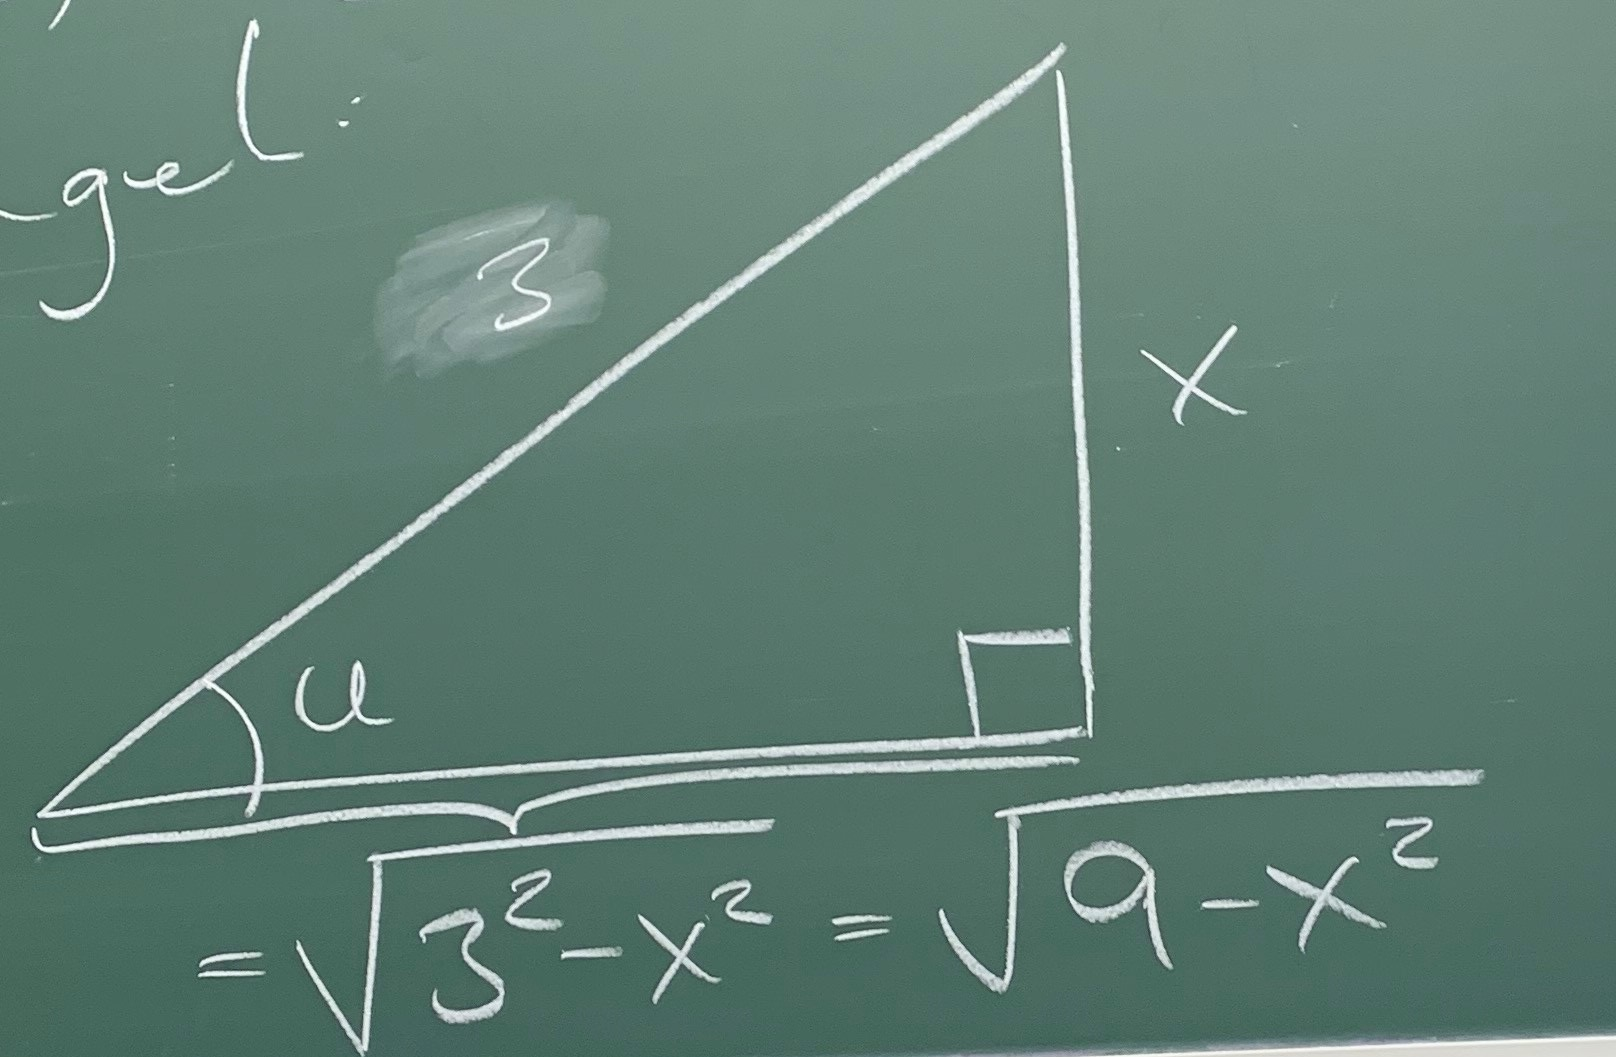
\includegraphics[scale=0.1]{lessons/lesson18/imgs/img01.jpg}

Värre kan det dock bli om antingen:
\begin{itemize}
    \item $f$ är obegränsad i någon punkt $x\in[a,b]$ %infoga bild 2 här
    \item $"a=-\infty"$ eller $b=\infty$ % infoga bild 3 här
\end{itemize}
Integraler som involverar någon eller båda egenheterna ovan kallas för \\
\underline{generaliserade integraler}.
De definieras naturligt genom gränsvärden.
Om $f$ är obegränsad i en punkt $c\in[a,b]$ så definieras integralern $\int_a^b f(x)\, dx$ som:
\begin{equation*}
    \int_a^b f(x)\, dx =\lim_{z\to c^-}\int_a^z f(x)\, dx+ \lim_{z\to c^+}\int_z^b f(x)\, dx
\end{equation*}
Om några av integrationsgränserna är obegränsad definieras integralen $\in_{-\infty}^b f(x)\, dx$
och $\int_a^\infty f(x)\, dx$ som:
\begin{equation*}
    \int_{-\infty}^b f(x)\, dx=\lim_{R\to \infty}\int_R^b f(x)\, dx\text{ och }\int_a^\infty f(x)\, dx=\lim_{R\to \infty}\int_a^R f(x)\, dx
\end{equation*}
För generaliserade integraler kan en av tre olika fall inträffa:
\begin{enumerate}
    \item Integralen existerar (blir ett tal)
    \item Integralen existerar inte (gränsvärdet går inte att beräkna)
    \item Integralen $=\infty$ eller $-\infty$
\end{enumerate}
Om $1.$ så kallas integralen \underline{konvergent}.
För $2.$ så säger man att integralen är \underline{divergent} och för $3.$ divergent mot $\infty$ eller $-\infty$.
Går ibland att avgöra konvergens/divergent genom att jämföra generaliserade integraler mot varandra.
Om $-\infty\leq a<b \leq\infty$ och $f$ och $g$ är kontinuerliga på $(a,b)$ så att $0\leq f(x)\leq g(x)$ så konvergerar $\int_a^b f(x)\, dx$ om $\int_a^b g(x)\, dx$ gör det.
På samma sätt om $\int_a^b f(x)\, dx$ divergerar mot $\infty$ så gör också $\int_a^b g(x)\, dx$ det.

\paragraph{Ex (6.5.17)} Beräkna $\int_1^e\frac{dx}{x\sqrt{\ln(x)}}$
\subparagraph{Lösning}
Integralen är generaliserad eftersom $\ln(1)=0\Rightarrow\frac{1}{1\cdot\ln(1)}=\infty$.
Det gäller att
\begin{equation*}
    \frac{d}{dx}(\sqrt{ln(x)})=
    \frac{1}{2}\cdot(\ln(x))^{-\frac{1}{2}}\cdot\frac{1}{x}=
    \frac{1}{2}\frac{1}{x\sqrt{\ln(x)}}
\end{equation*}
\begin{equation*}
    \text{så }\int_1^e\frac{dx}{x\sqrt{\ln(x)}}=
    \lim_{z\to 1^+}\int_z^e\frac{dx}{x\sqrt{\ln(x)}}=
    \lim_{z\to 1^+}[2\sqrt{\ln(x)}]_z^e=
\end{equation*}
\begin{equation*}
    \lim_{z\to 1^+}2(\sqrt{\ln(e)}-\sqrt{\ln(z)})=
    2(1-0)=2\Rightarrow\text{Konvergent! }\Box
\end{equation*}

\paragraph{Ex (6.5.18)} Samma som innan för $\int_e^\infty\frac{dx}{x(\ln(x))^2}$
\subparagraph{Lösning}
\begin{equation*}
    \int_e^\infty\frac{dx}{x(\ln(x))^2}=
    \left\lbrace
    \begin{matrix}[c|c]
        u=\ln(x)            & x=e\Rightarrow u=1           \\
        du=\frac{1}{x}\, dx & x=\infty\Rightarrow u=\infty
    \end{matrix}
    \right.=
    \int_1^\infty\frac{1}{u^2}\, du=
\end{equation*}
\begin{equation*}
    \lim_{R\to\infty}\int_1^R\frac{1}{u^2}\, du=
    \lim_{R\to\infty}\int_1^R[-\frac{1}{u}]_1^R=
    \lim_{R\to\infty}((-\frac{1}{R})-(-\frac{1}{1}))=
    1\Rightarrow\text{Konvergent! }\Box
\end{equation*}
~\\
Några generaliserade integraler som är bra att känna till för att avgöra konvergens/divergens genom jämförelse är det så kallade "p-integralerna".
\begin{enumerate}
    \item $\int_a^\infty x^{-p}\, dx=
              \left\lbrace
              \begin{matrix}
                  \text{konvergerar mot }\frac{a^{1-p}}{p-1}\text{\underline{ om }} p>1 \\
                  \text{divergerar mot }\infty \text{ om } 0<p\leq 1
              \end{matrix}
              \right.$
    \item $\int_0^a x^{-p}\, dx=
              \left\lbrace
              \begin{matrix}
                  \text{konvergerar mot }\frac{a^{1-p}}{1-p}\text{\underline{ om }} 0<p<1 \\
                  \text{divergerar mot }\infty \text{ om } p\geq 1
              \end{matrix}
              \right.$
\end{enumerate}
för $0<a<\infty$.\\
%infoga bild 4
%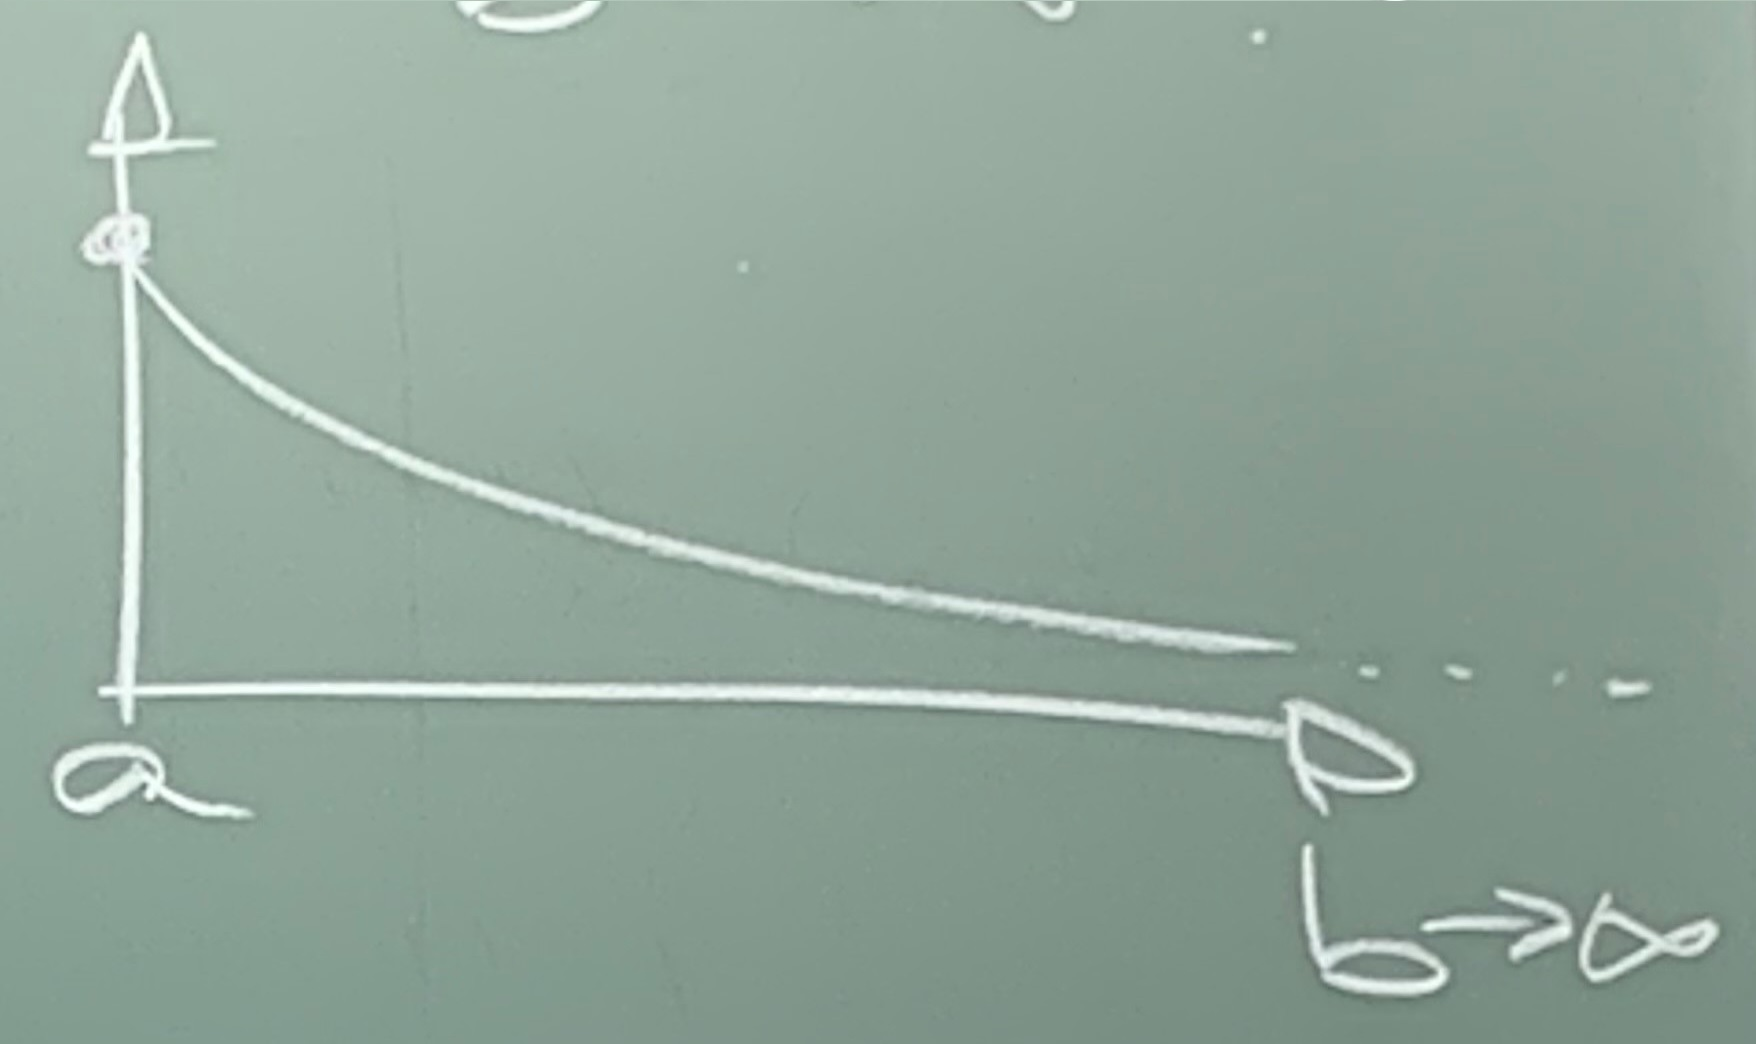
\includegraphics[scale=0.1]{lessons/lesson18/imgs/img04.jpg}

\chapter{Numerisk integration}
%Numerisk integration kommer inte på tentan 👀
Viktigt att kunna beräkna bra approximationer av integraler numeriskt.
Finns olika typer av algoritmer/metoder.

\section{Mittpunktsmetoden}
Approximera $\int_a^b f(x)\, dx$ som en Riemann-summa av staplar av samma bredd vars höjd motsvarar funktionens värde vid stapelns mittpunkt.\\
%infoga bild 5
%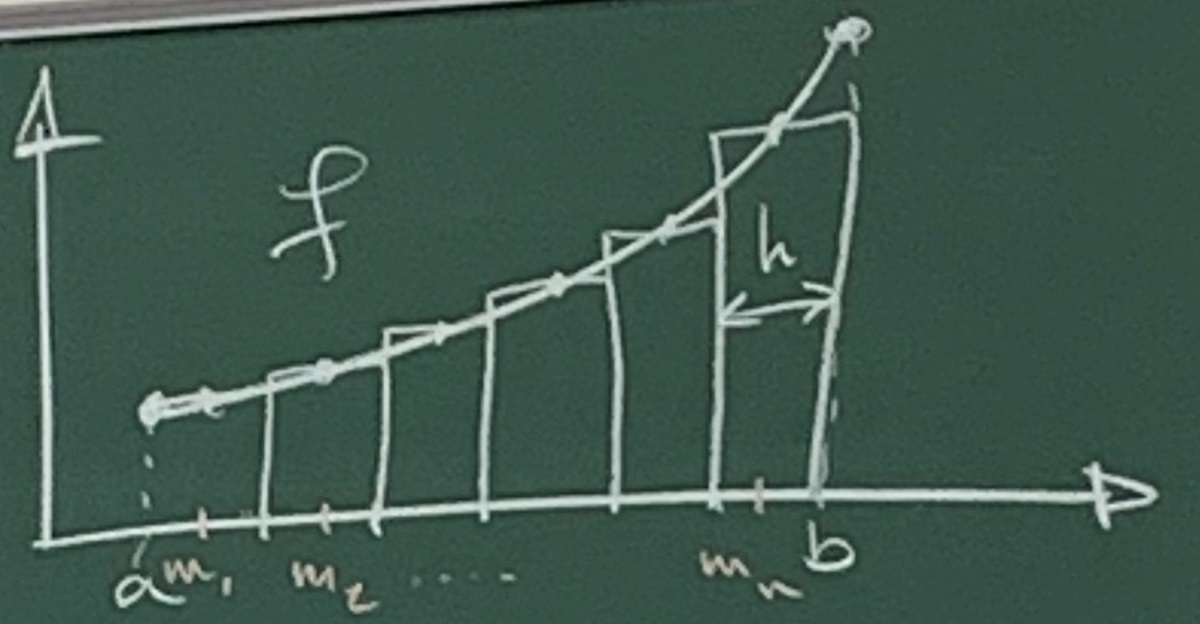
\includegraphics[]{lessons/lesson18/imgs/img05.jpg}
\begin{equation*}
    \Rightarrow \int_a^b f(x)\, dx \approx
    f(m_1)\cdot h+f(m_2)\cdot h+...+f(m_n)\cdot h=
    h\cdot\sum_i^n f(m_i)=
    M_n
\end{equation*}
Ju mindre bredd $h>0$ desto bättre approximation.

\section{Trapetsmetoden}
Istället för att som i mittpunktsmetoden använda en punkt per stapel för höjden (mittpunkten), används stapelsn ändpunkter och linjärapprox. funktionen.\\
%infoga bild 6
%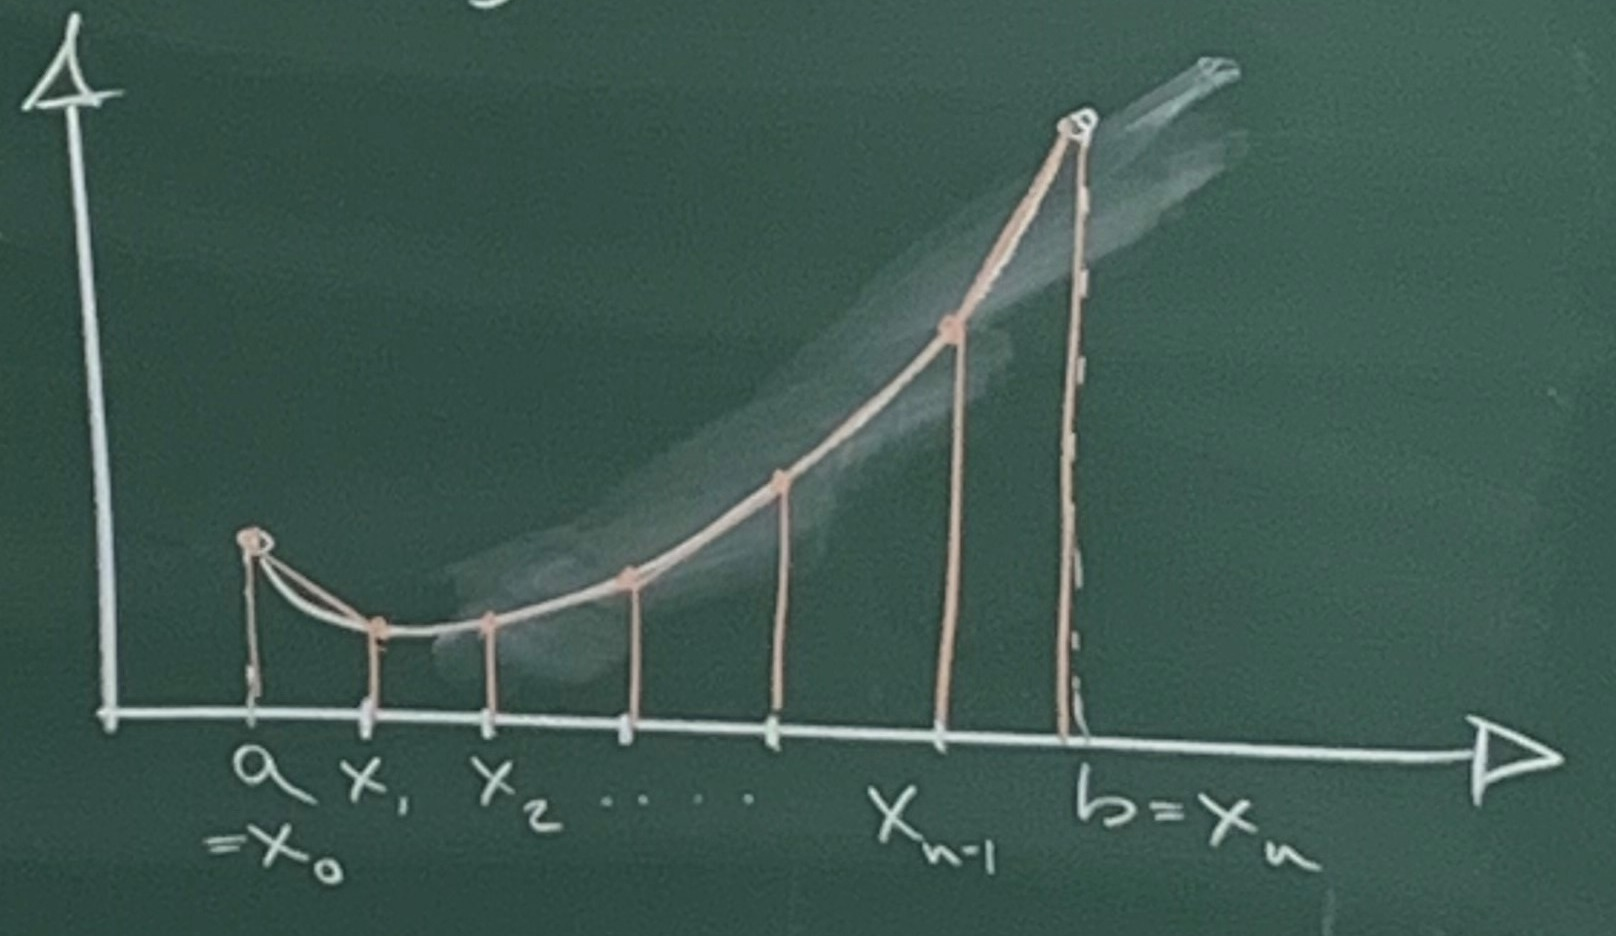
\includegraphics[scale=0.1]{lessons/lesson18/imgs/img06.jpg}\\
För stapel $i$ $(0<i<n)$ gäller:
%infoga bild 7
%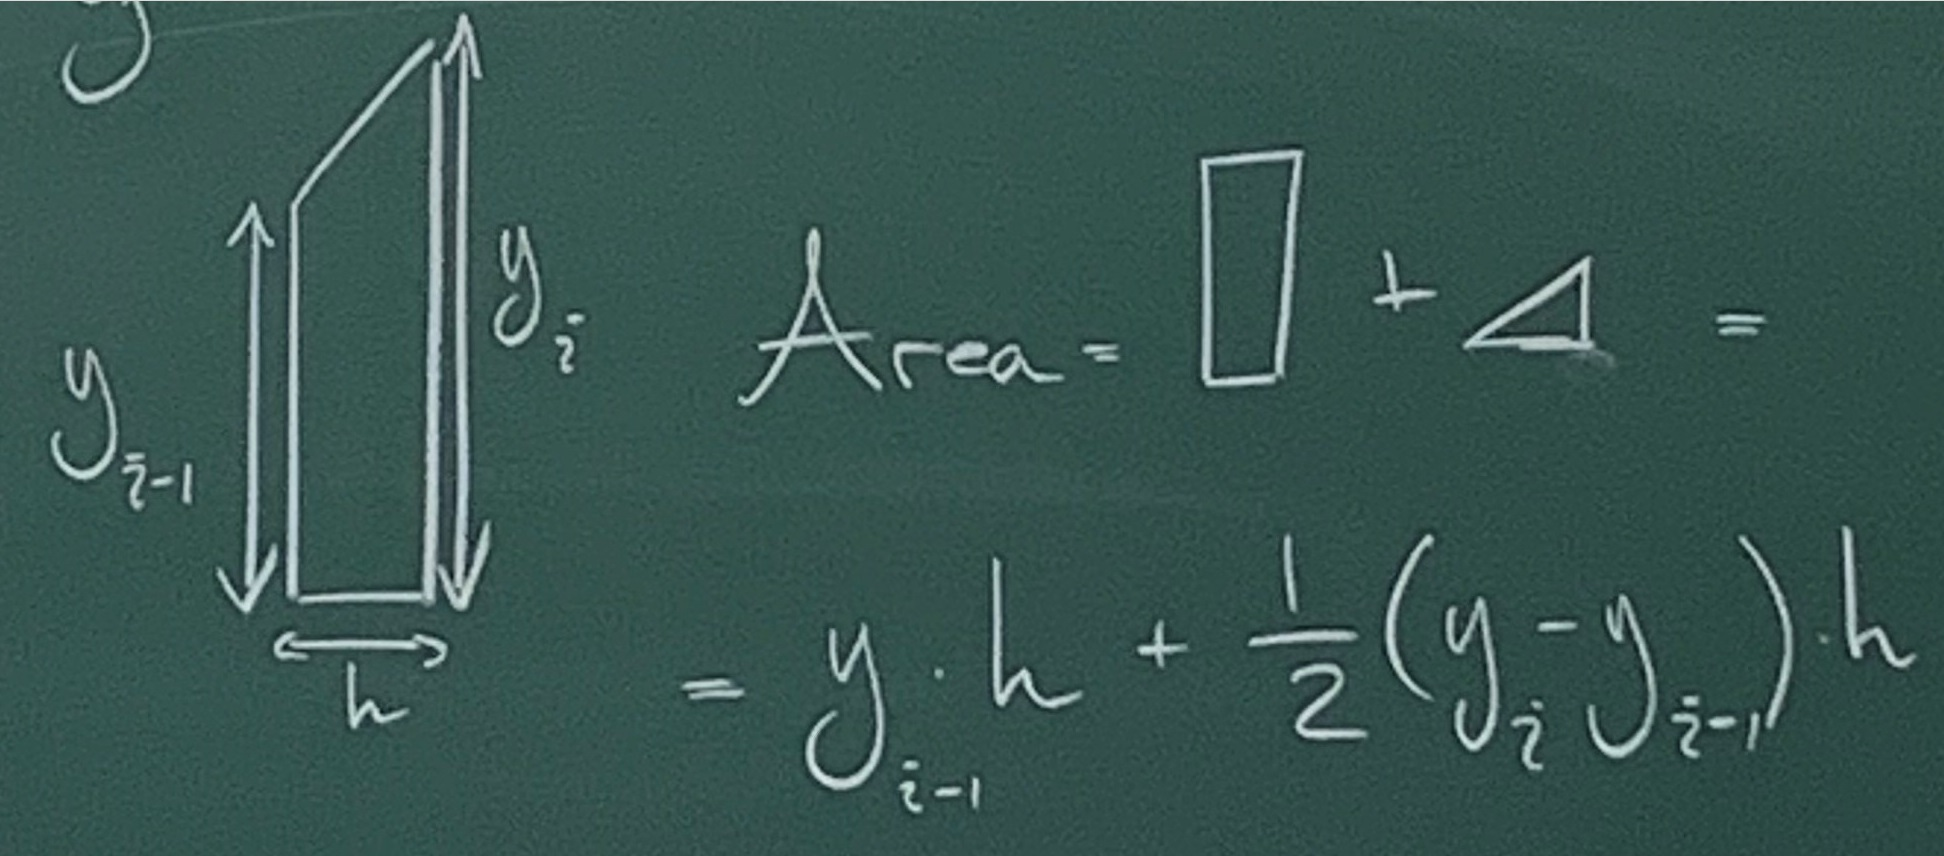
\includegraphics[scale=0.1]{lessons/lesson18/imgs/img07.jpg}
\begin{equation*}
    \Rightarrow \int_a^b f(x)\, dx\approx
    y_0\cdot h+\frac{1}{2}(y_1-y_0)\cdot h+y_1\cdot h+\frac{1}{2}(y_2-y_1)\cdot h+...=
\end{equation*}
\begin{equation*}
    h\cdot(\frac{1}{2}y_0+y_1+y_2+...+y_{n-1}+\frac{1}{2}y_n)=T_n
\end{equation*}
Vilken metod är bäst?
Man kan visa att:
\begin{itemize}
    \item Trapetsmetoden $|\int_a^b f(x)\, dx-M_n|\leq \frac{k\cdot(b-a)^3}{12n^2}$
    \item Mittpunktsmetoden $|\int_a^b f(x)\, dx-T_n\leq\frac{k\cdot(b-a)^3}{24n^2}$
\end{itemize}
för ett tal $K$ som hänger ihop med $f$.
Alltså är:
\begin{itemize}
    \item Trapetsmetoden $\int_a^b f(x)\, dx=M_n+O(\frac{1}{n^2})$
    \item Mittpunktsmetoden $\int_a^b f(x)\, dx=T_n+O(\frac{1}{n^2})$
\end{itemize}
dvs. dom är lika bra!\\
klar förbätttring fås genom att använda både mittpunkten och ändpunkterna och approximera $f$ i stapeln med en andragradskurva genom punkterna.
\section{Simpsons regel}
%infoga bild 8
%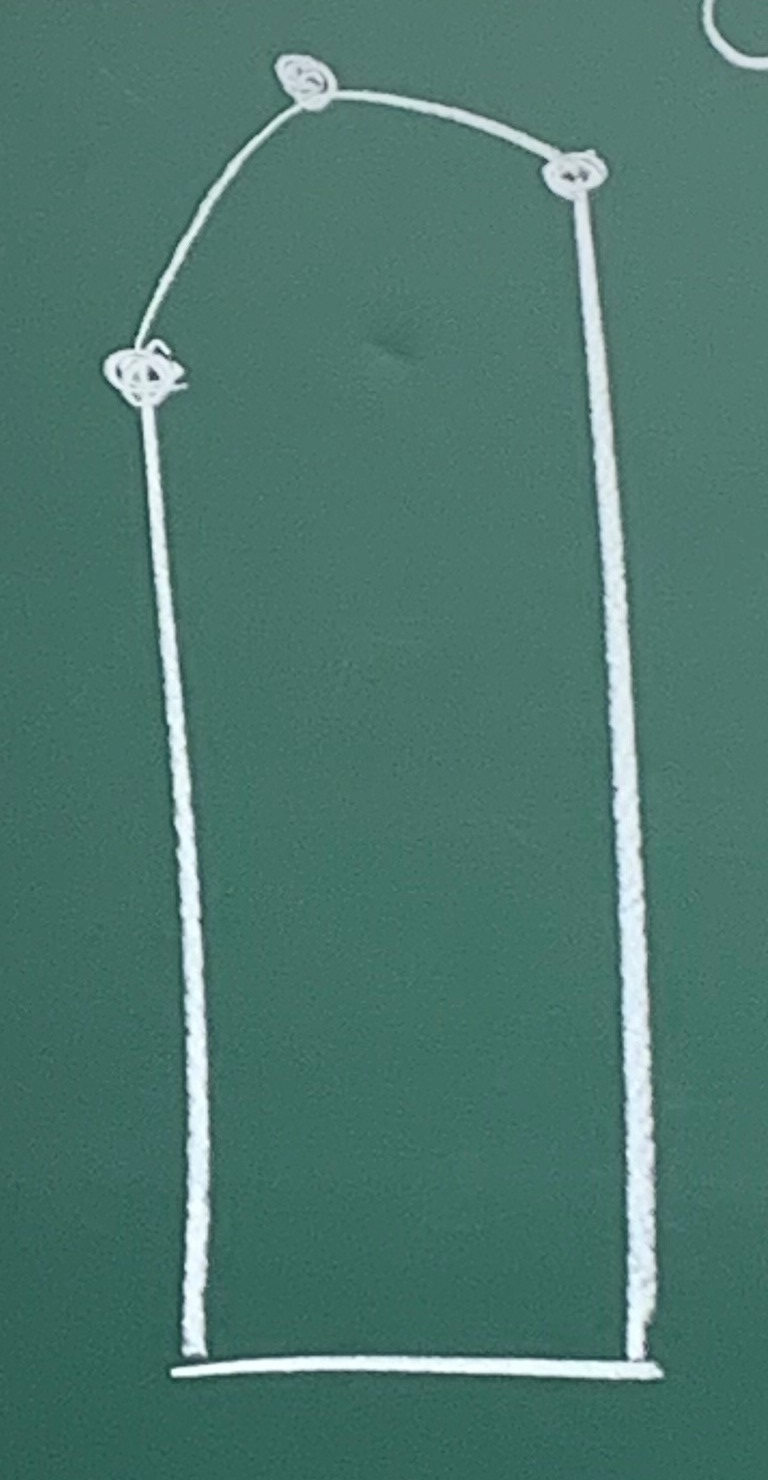
\includegraphics[scale=0.1]{lessons/lesson18/imgs/img08.jpg}
Man kan visa att Simpson-approximation innebär ett fel av storleksordning $O(\frac{1}{n^4})$ dvs.
\begin{equation*}
    \int_a^b f(x)\, dx=S_n+O(\frac{1}{n^4})
\end{equation*}
\chapter{Tillämpningar av integraler}
Vi har följande geometriska tolkning av integraler:\\
$\int_a^bf(x)\, dx=$"arean med tecken under grafen till $f(x)$ begränsad av $x$-axeln"\\
%infoga bild 1
%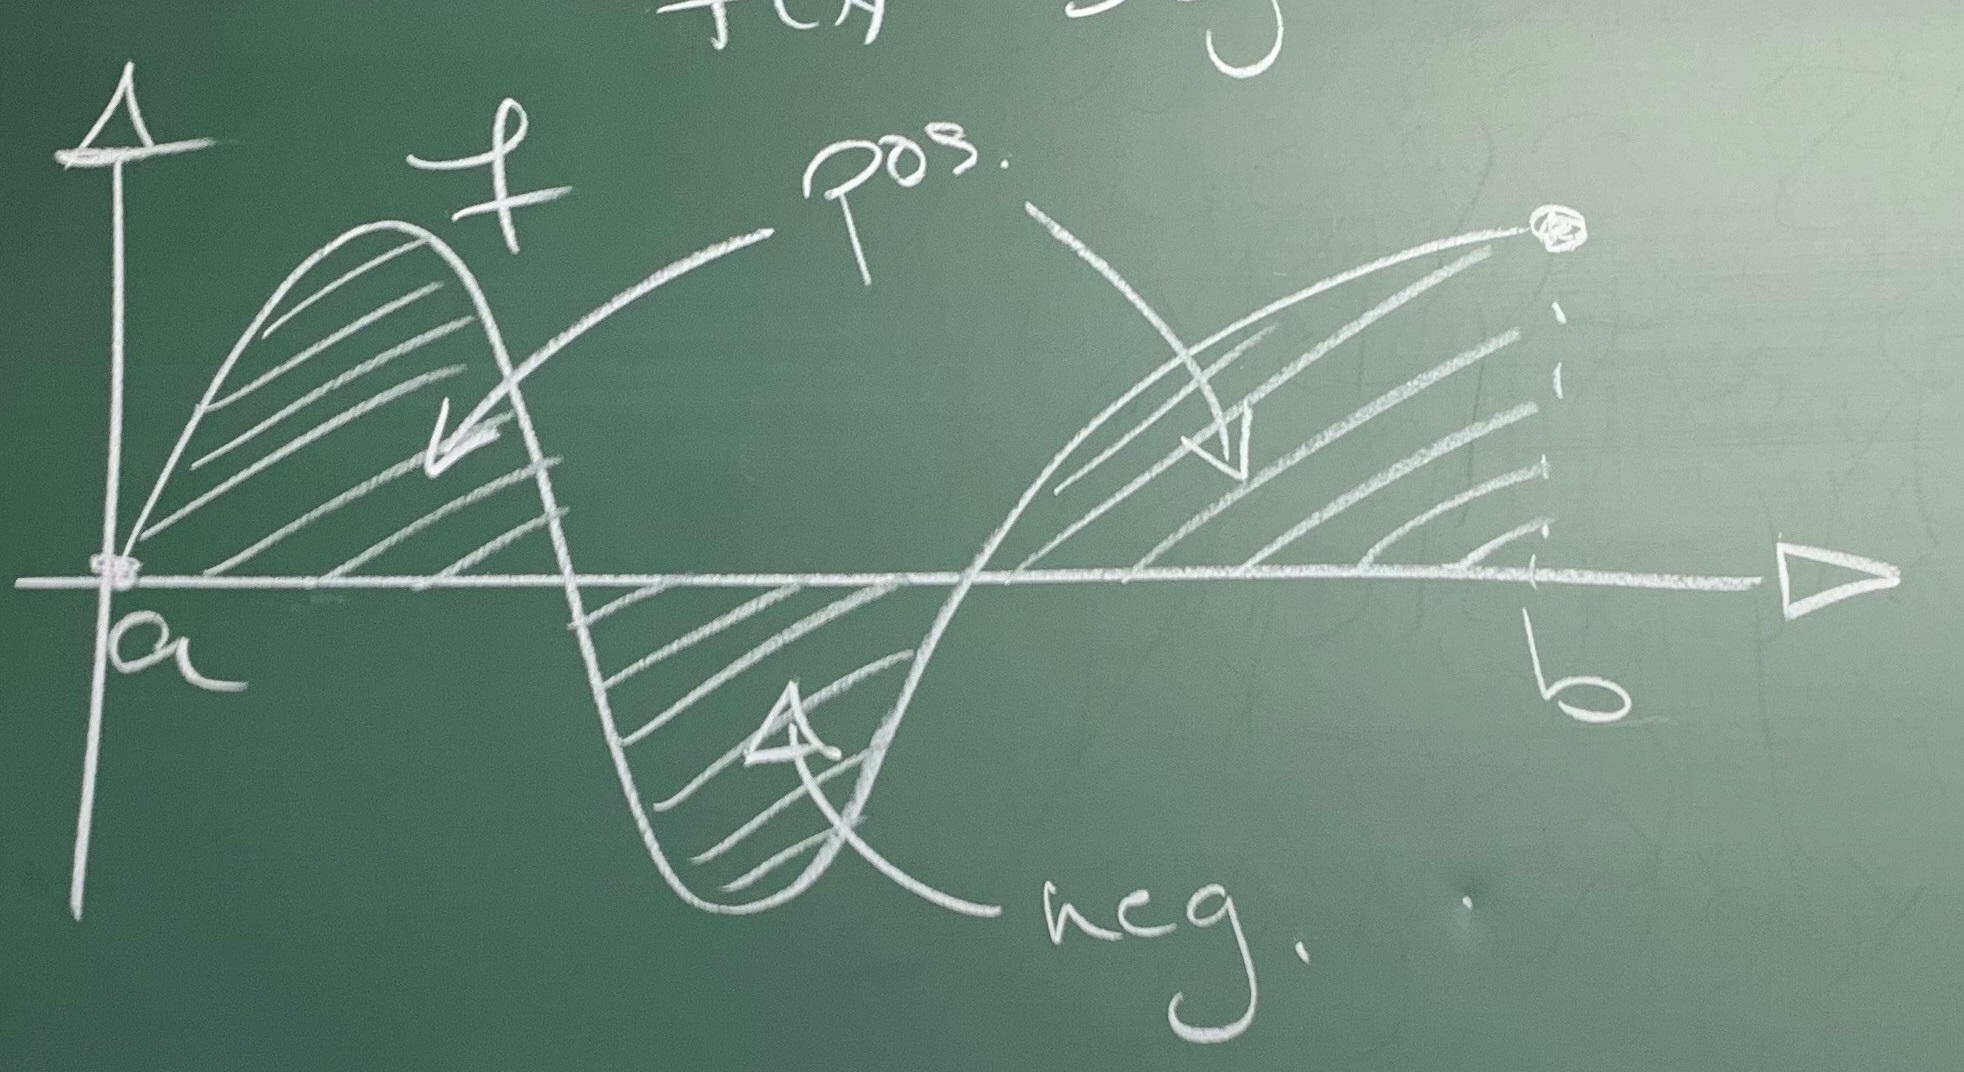
\includegraphics[scale=0.1]{lessons/lesson19/imgs/img01.jpg}
Om man vill ha totalarean (dvs arean utan tecken) är det bara att integrera $|f(x)|$ istället.
\begin{equation*}
    \int_a^b|f(x)|\, dx=\text{"totala arean under grafen"}
\end{equation*}
På liknande sätt kan man beräkna arean mellan två grafer.
%infoga bild 2
%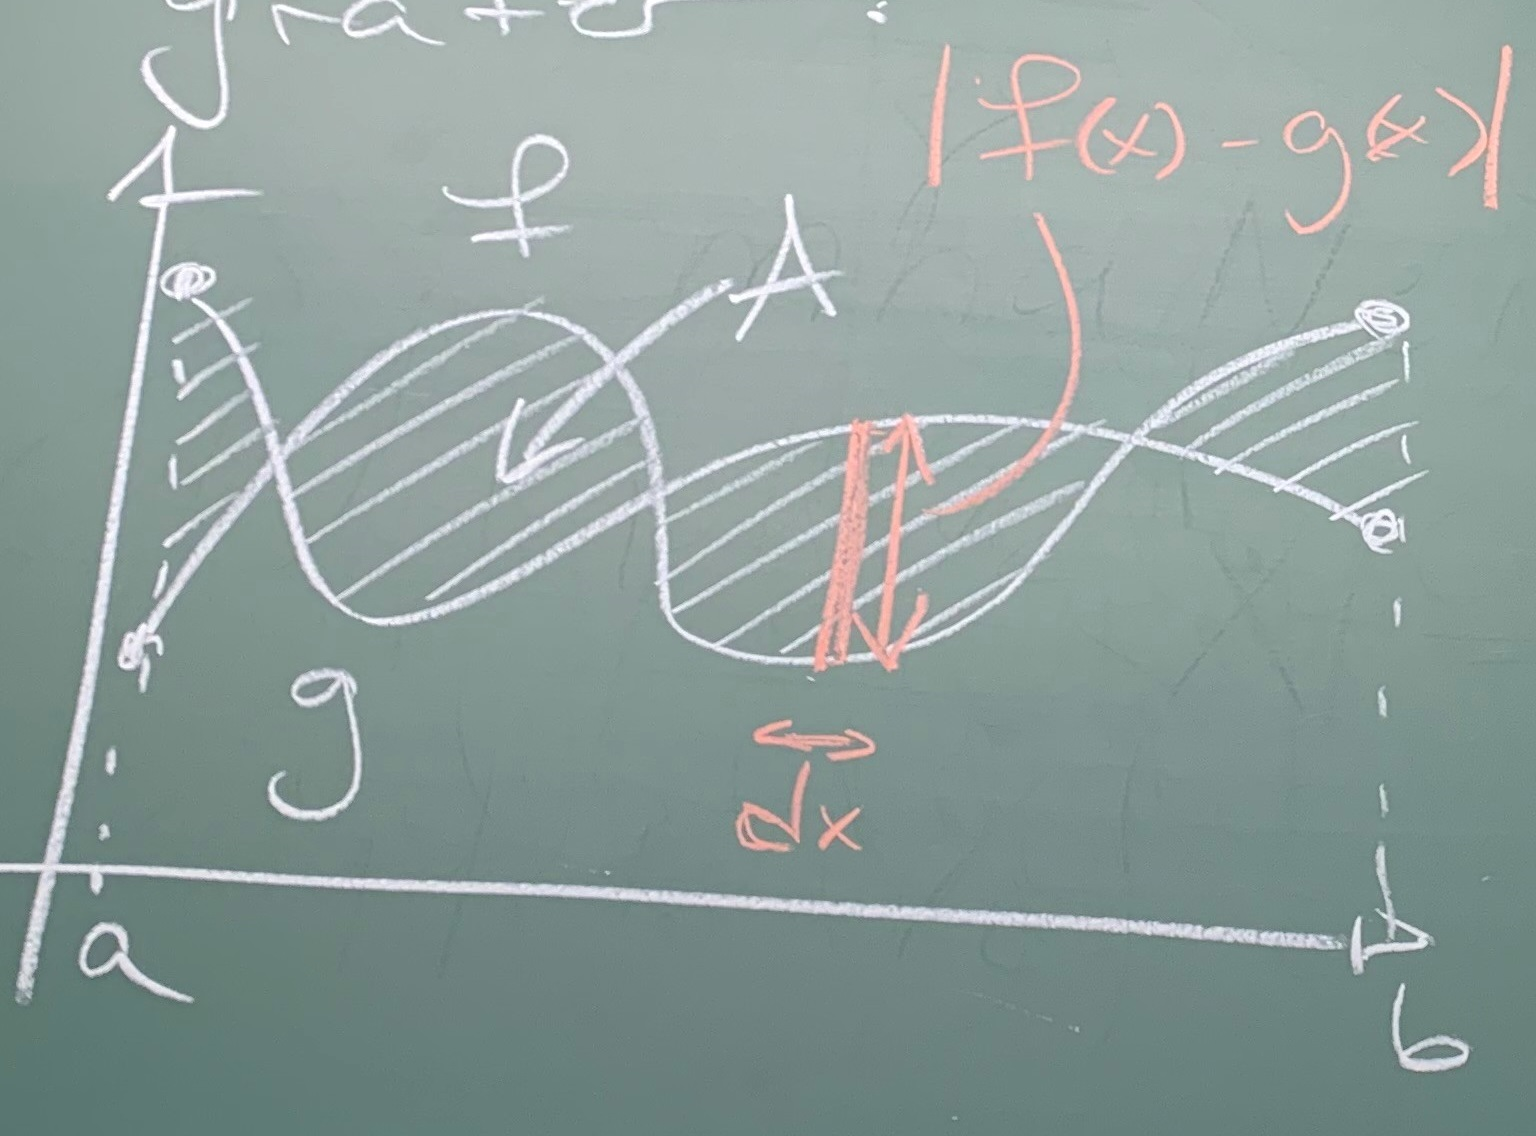
\includegraphics[scale=0.1]{lessons/lesson19/imgs/img02.jpg}
\begin{equation*}
    A=\int_a^b|f(x)-g(x)|\, dx
\end{equation*}
Metoden med att integrera infinitesimala element, som till exempel $|f(x)-g(x)|\,dx$, är mycket användbar.

\section{Volymberäkning}
Att beräkna volymer med integraler kräver i allmänhet teori från från flervariabelanalys eftersom det grundläggande infinitesimala elementet är en liten kub med volym $dV=dx\,dy\,dz$.
%infoga bild 3
%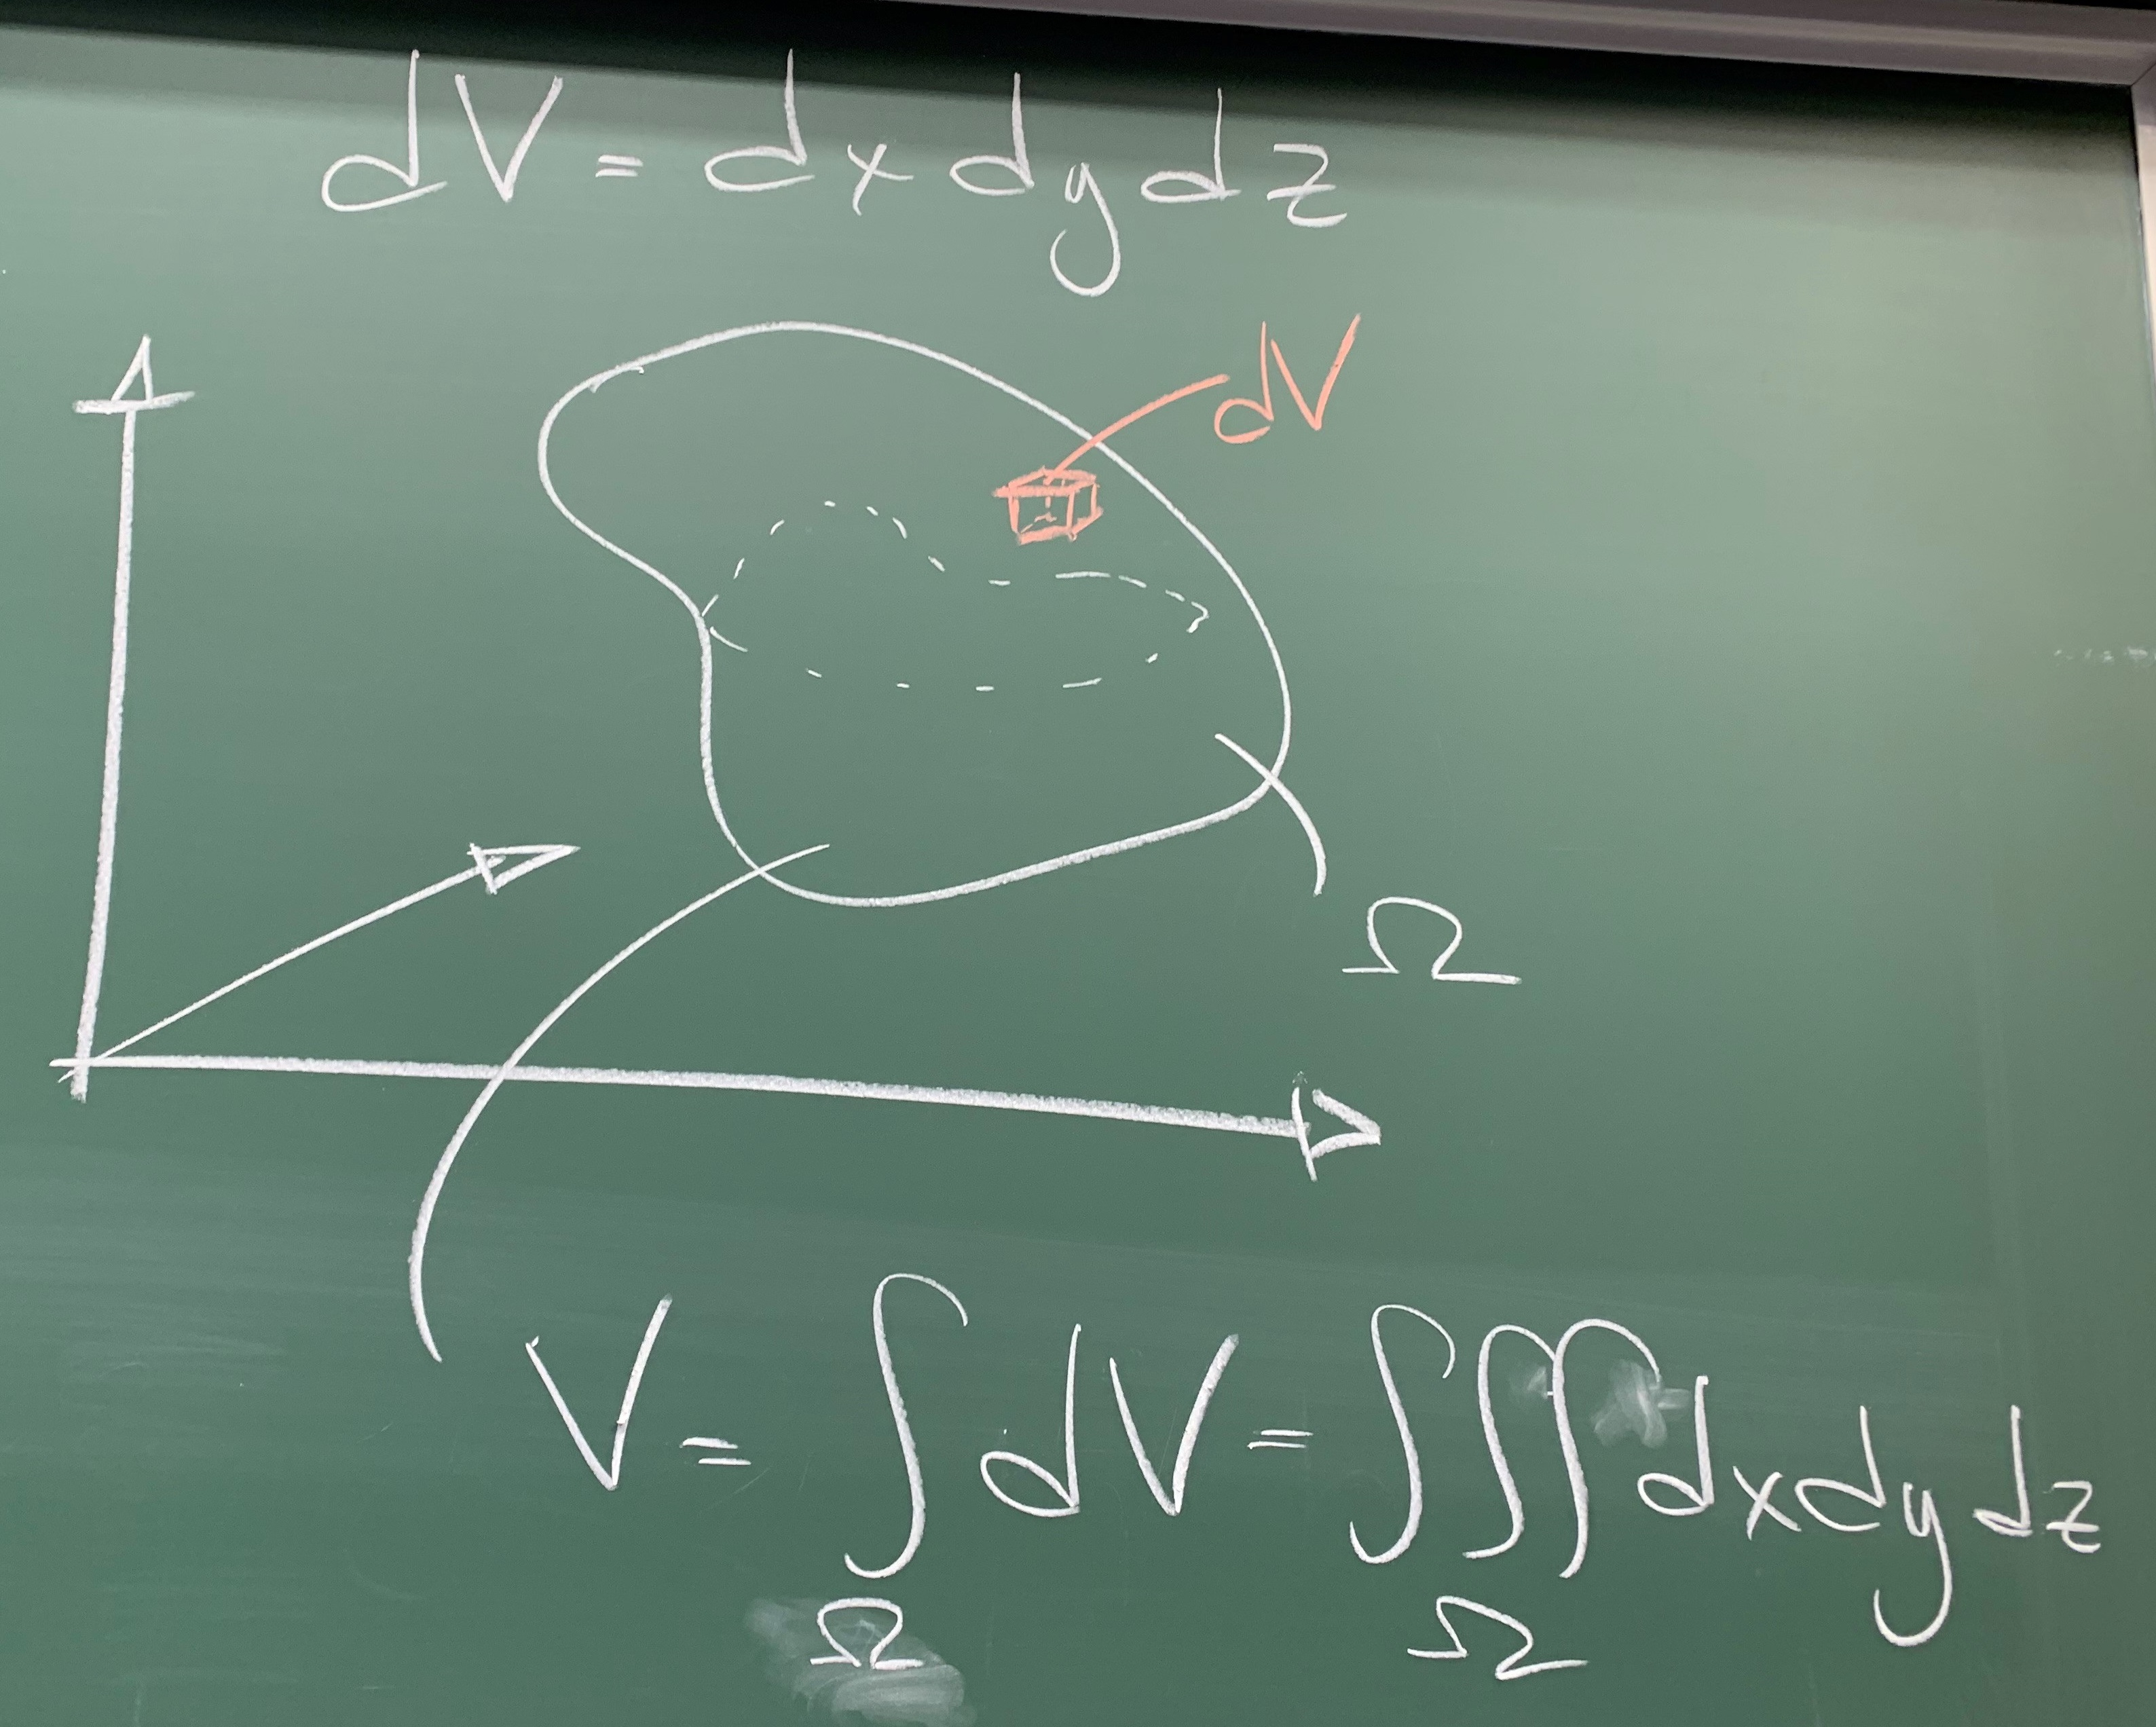
\includegraphics[scale=0.1]{lessons/lesson19/imgs/img03.jpg}
Ibland klarar man sig dock med vanliga enkelintegraler om man kan skriva $dV=A(x)dx$, där $A(x)$ beskriver arean av en "skiva" och $dx$ är skivans tjocklek.
Går om volymen man vill beräkna uppvisar någon form av symmetri.
%infoga bild 4
%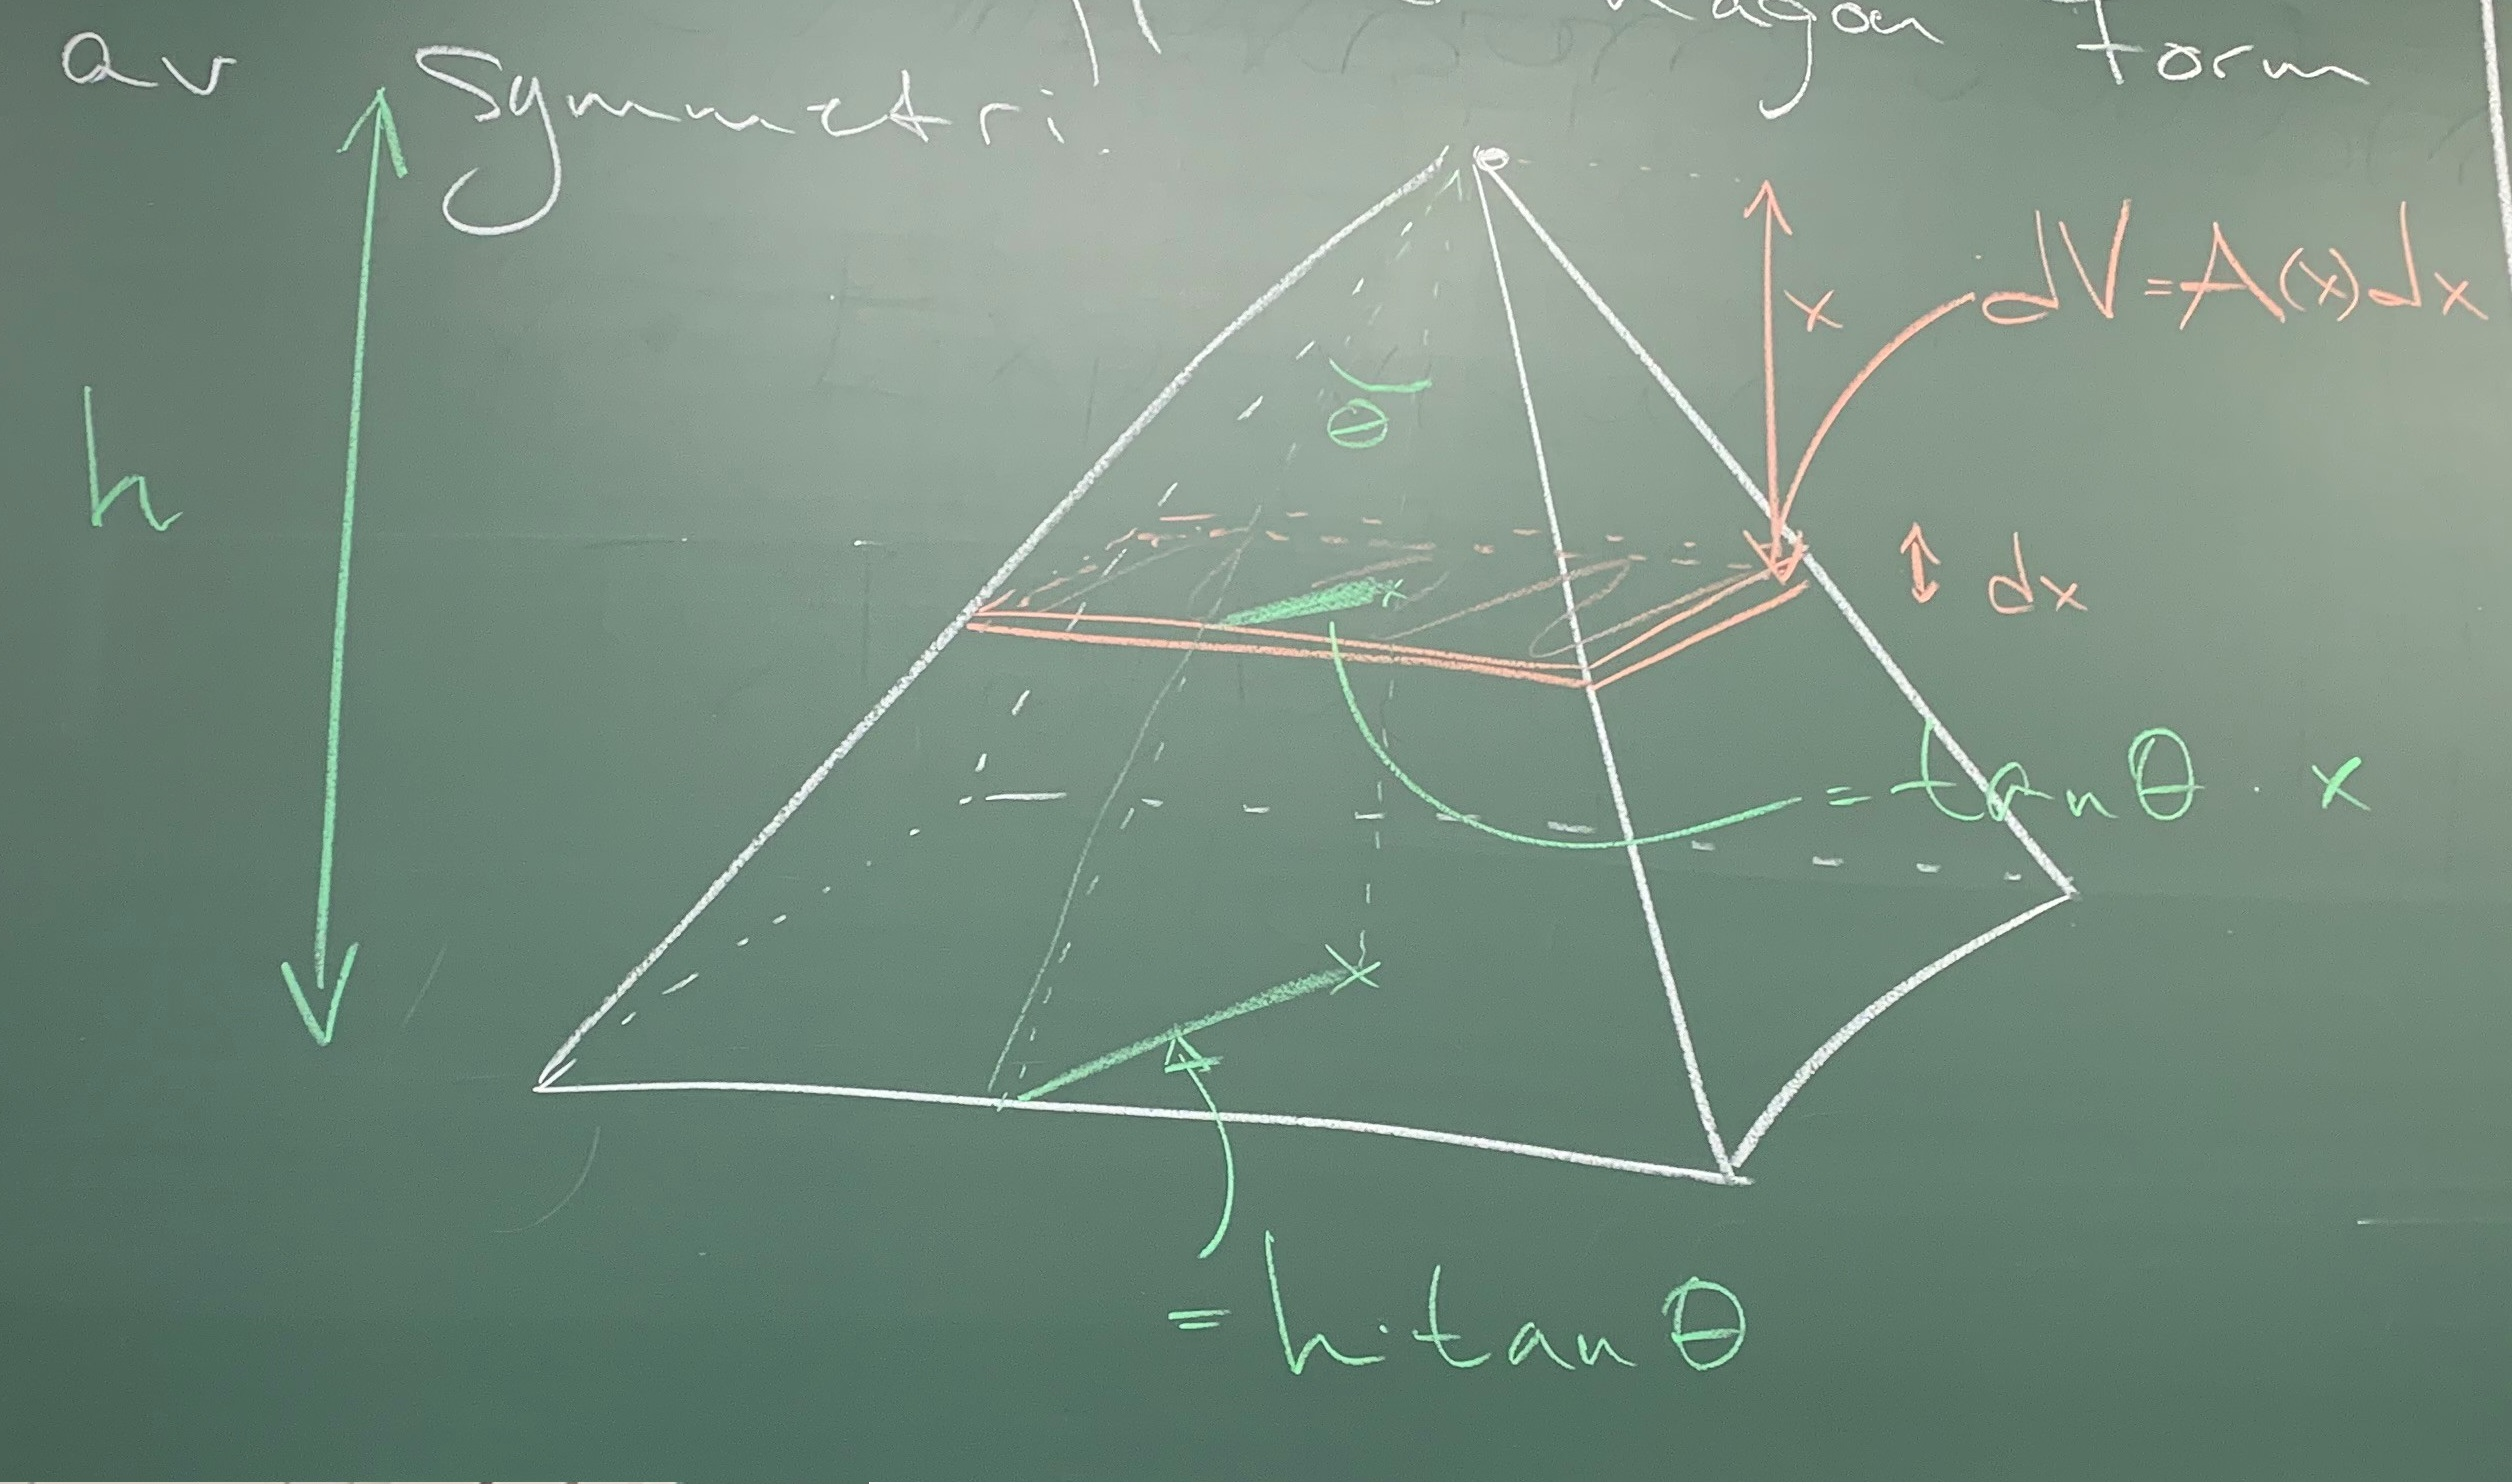
\includegraphics[scale=0.1]{lessons/lesson19/imgs/img04.jpg}
\begin{equation*}
    A(x)=(2\cdot x\cdot\tan(\theta))^2=4x^2\tan^2(\theta)\Rightarrow
    V=\int\, dV=
    \int A(x)\, dx=
\end{equation*}
\begin{equation*}
    \int_0^h 4x^2\tan^2(\theta)\, dx=
        [\frac{4}{3}x^3\tan^2(\theta)]_0^h=
    \frac{4}{3}h^3\cdot\tan^2(\theta)=
    \frac{h}{3}4h^2\tan^2(\theta)=
\end{equation*}
\begin{equation*}
    \{4h^2\tan^2(\theta)="basytan"=b\}=
    \frac{h\cdot b}{3}
\end{equation*}
Ibland uppvisar volymer rotationssymmetri med antingen $x$- eller $y$-axeln och då utnyttjas detta genom rotationssymmetriska element.
%infoga bild 5
%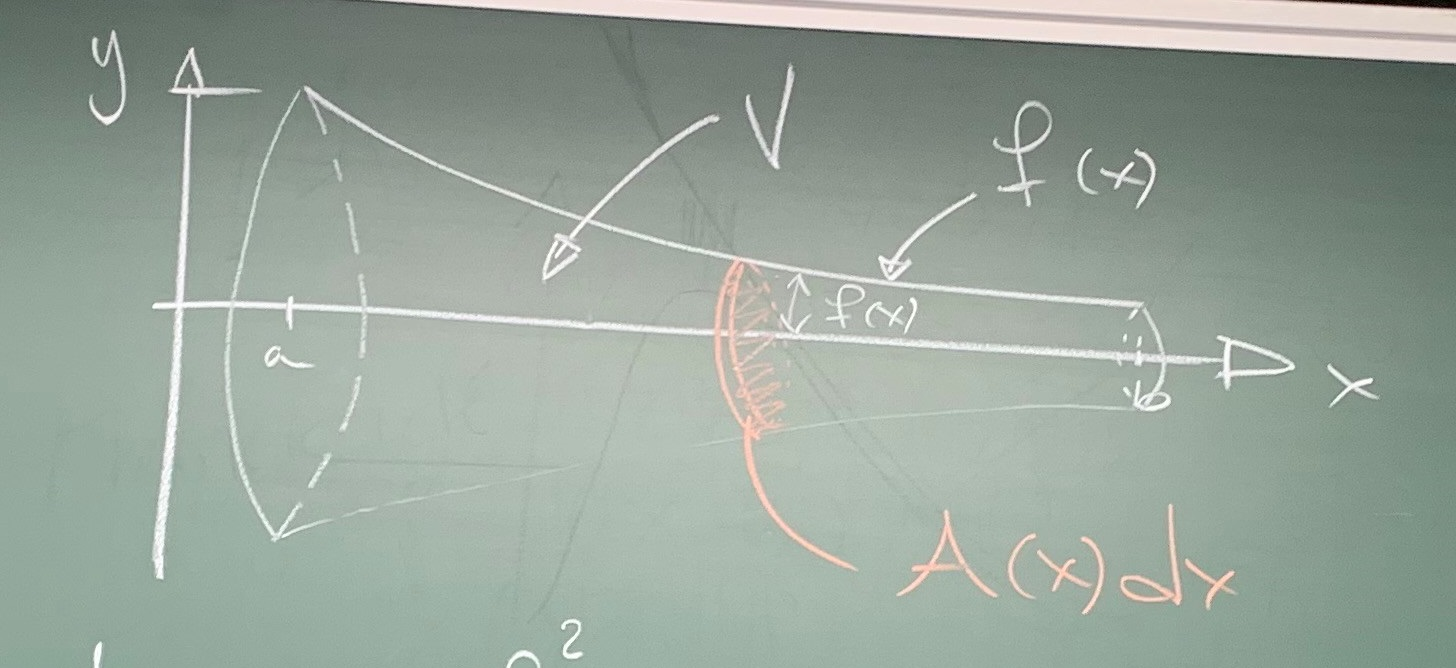
\includegraphics[scale=0.1]{lessons/lesson19/imgs/img05.jpg}
\begin{equation*}
    A(x)=f^2(x)\cdot\pi\Rightarrow
    V=\int dV=\int_a^bf^2(x)\overline{u}\, dx
\end{equation*}
Liknande konstruktion runt $y$-axeln.

\paragraph*{Ex (7.1.16)} Bestäm volymen av den kropp som fås genom att rotera en cirkelskiva runt en godtycklig tangentlinje.
\subparagraph{Lösning}
%infoga bild 6
%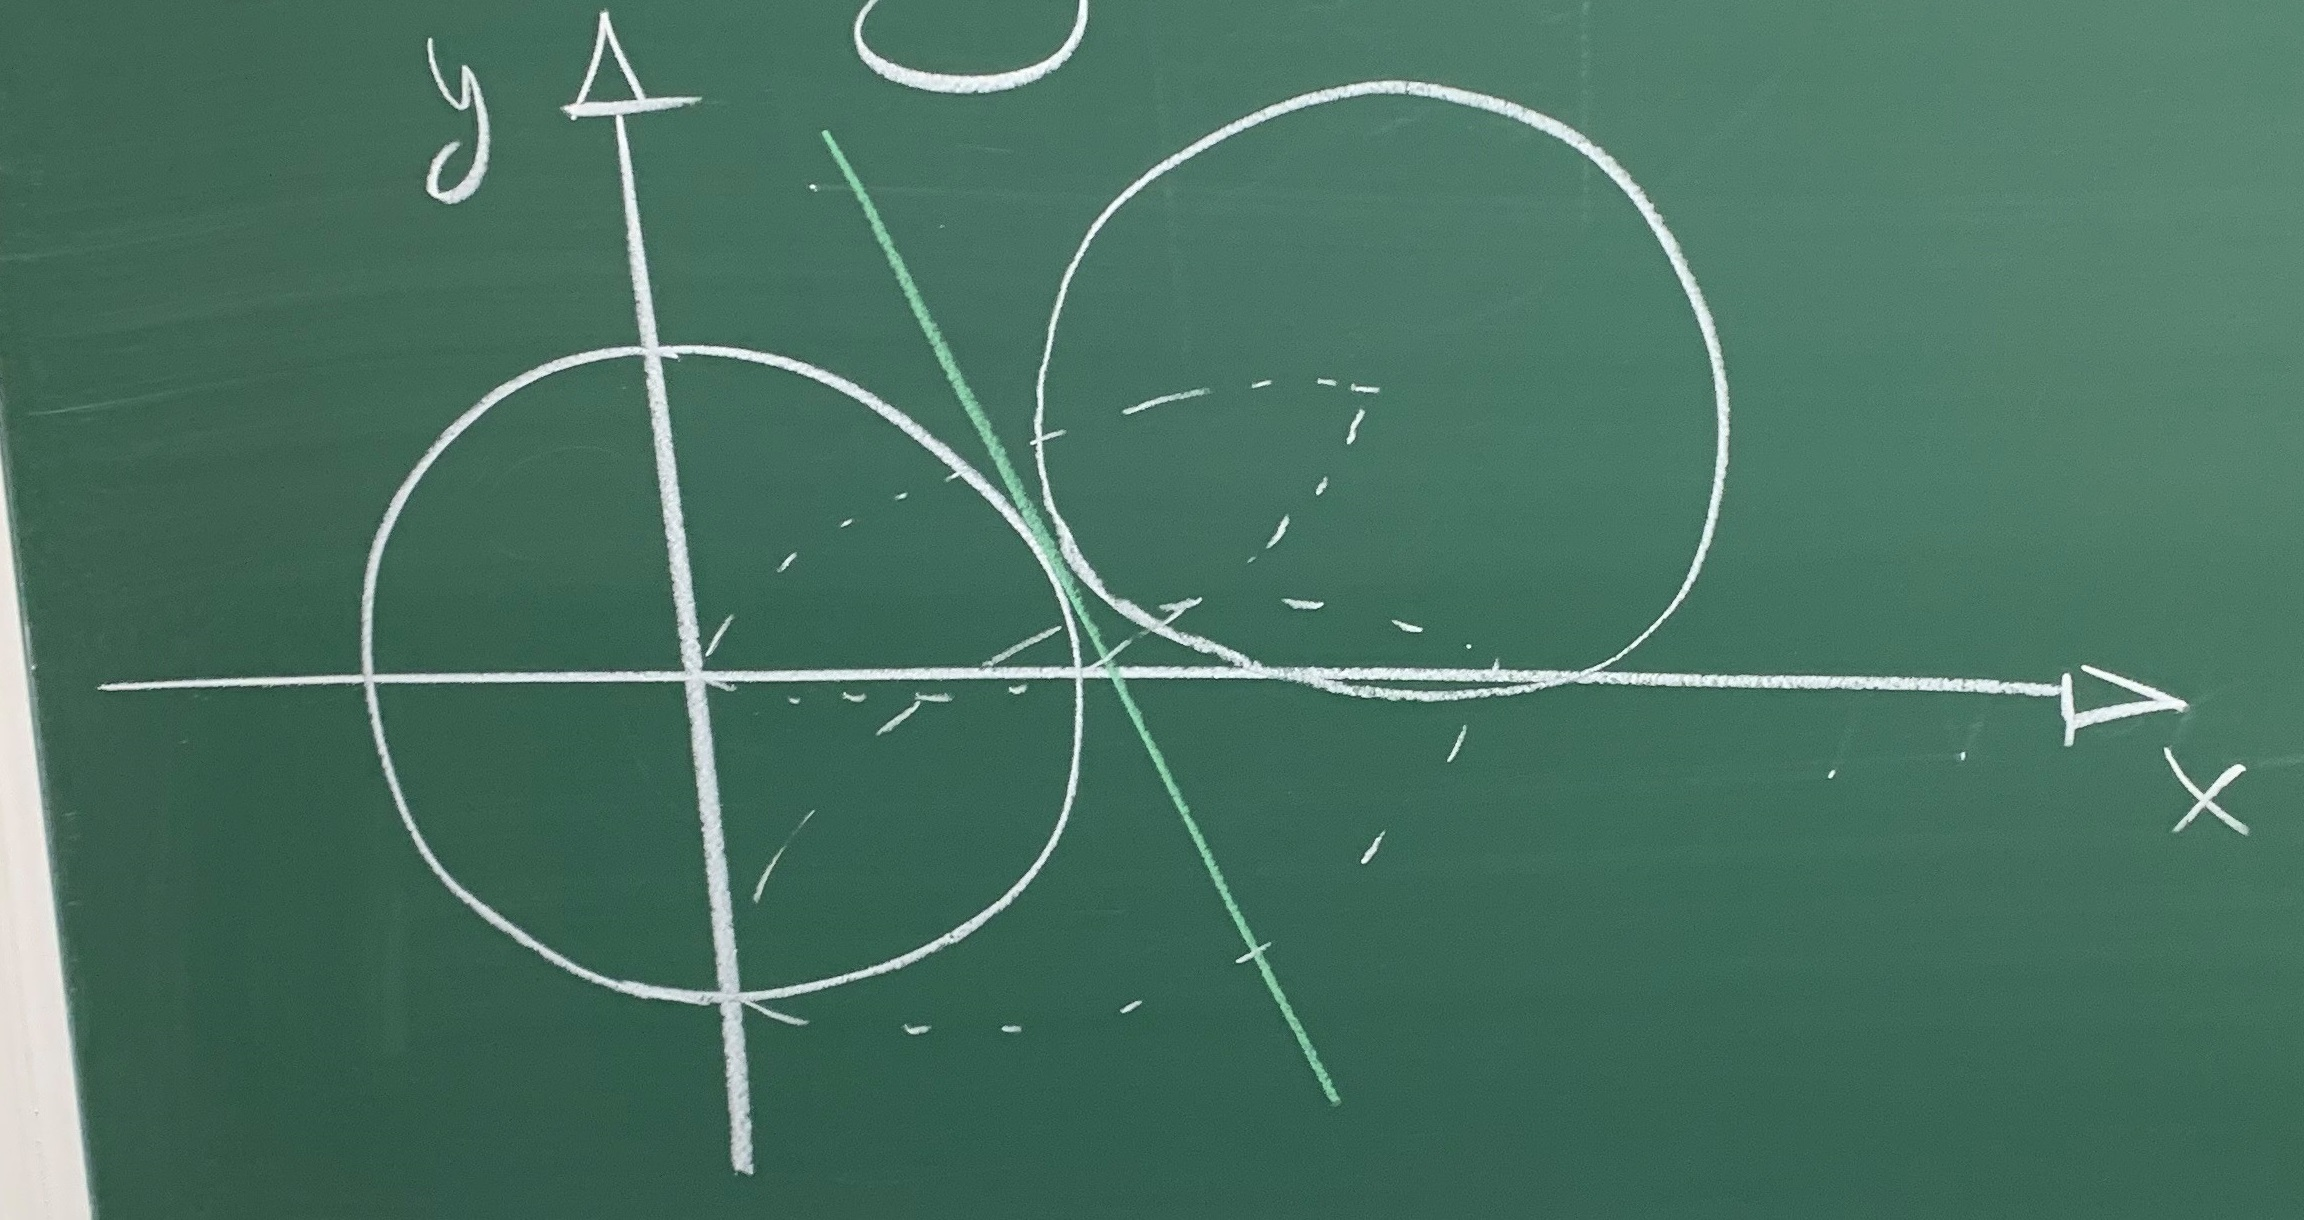
\includegraphics[scale=0.1]{lessons/lesson19/imgs/img06.jpg}
Volymen är av symmetriskäl oberoende av tangentlinje, så välj linjen $x=r$, där $r$ är cirkelskivans radie.
%infoga bild 7
%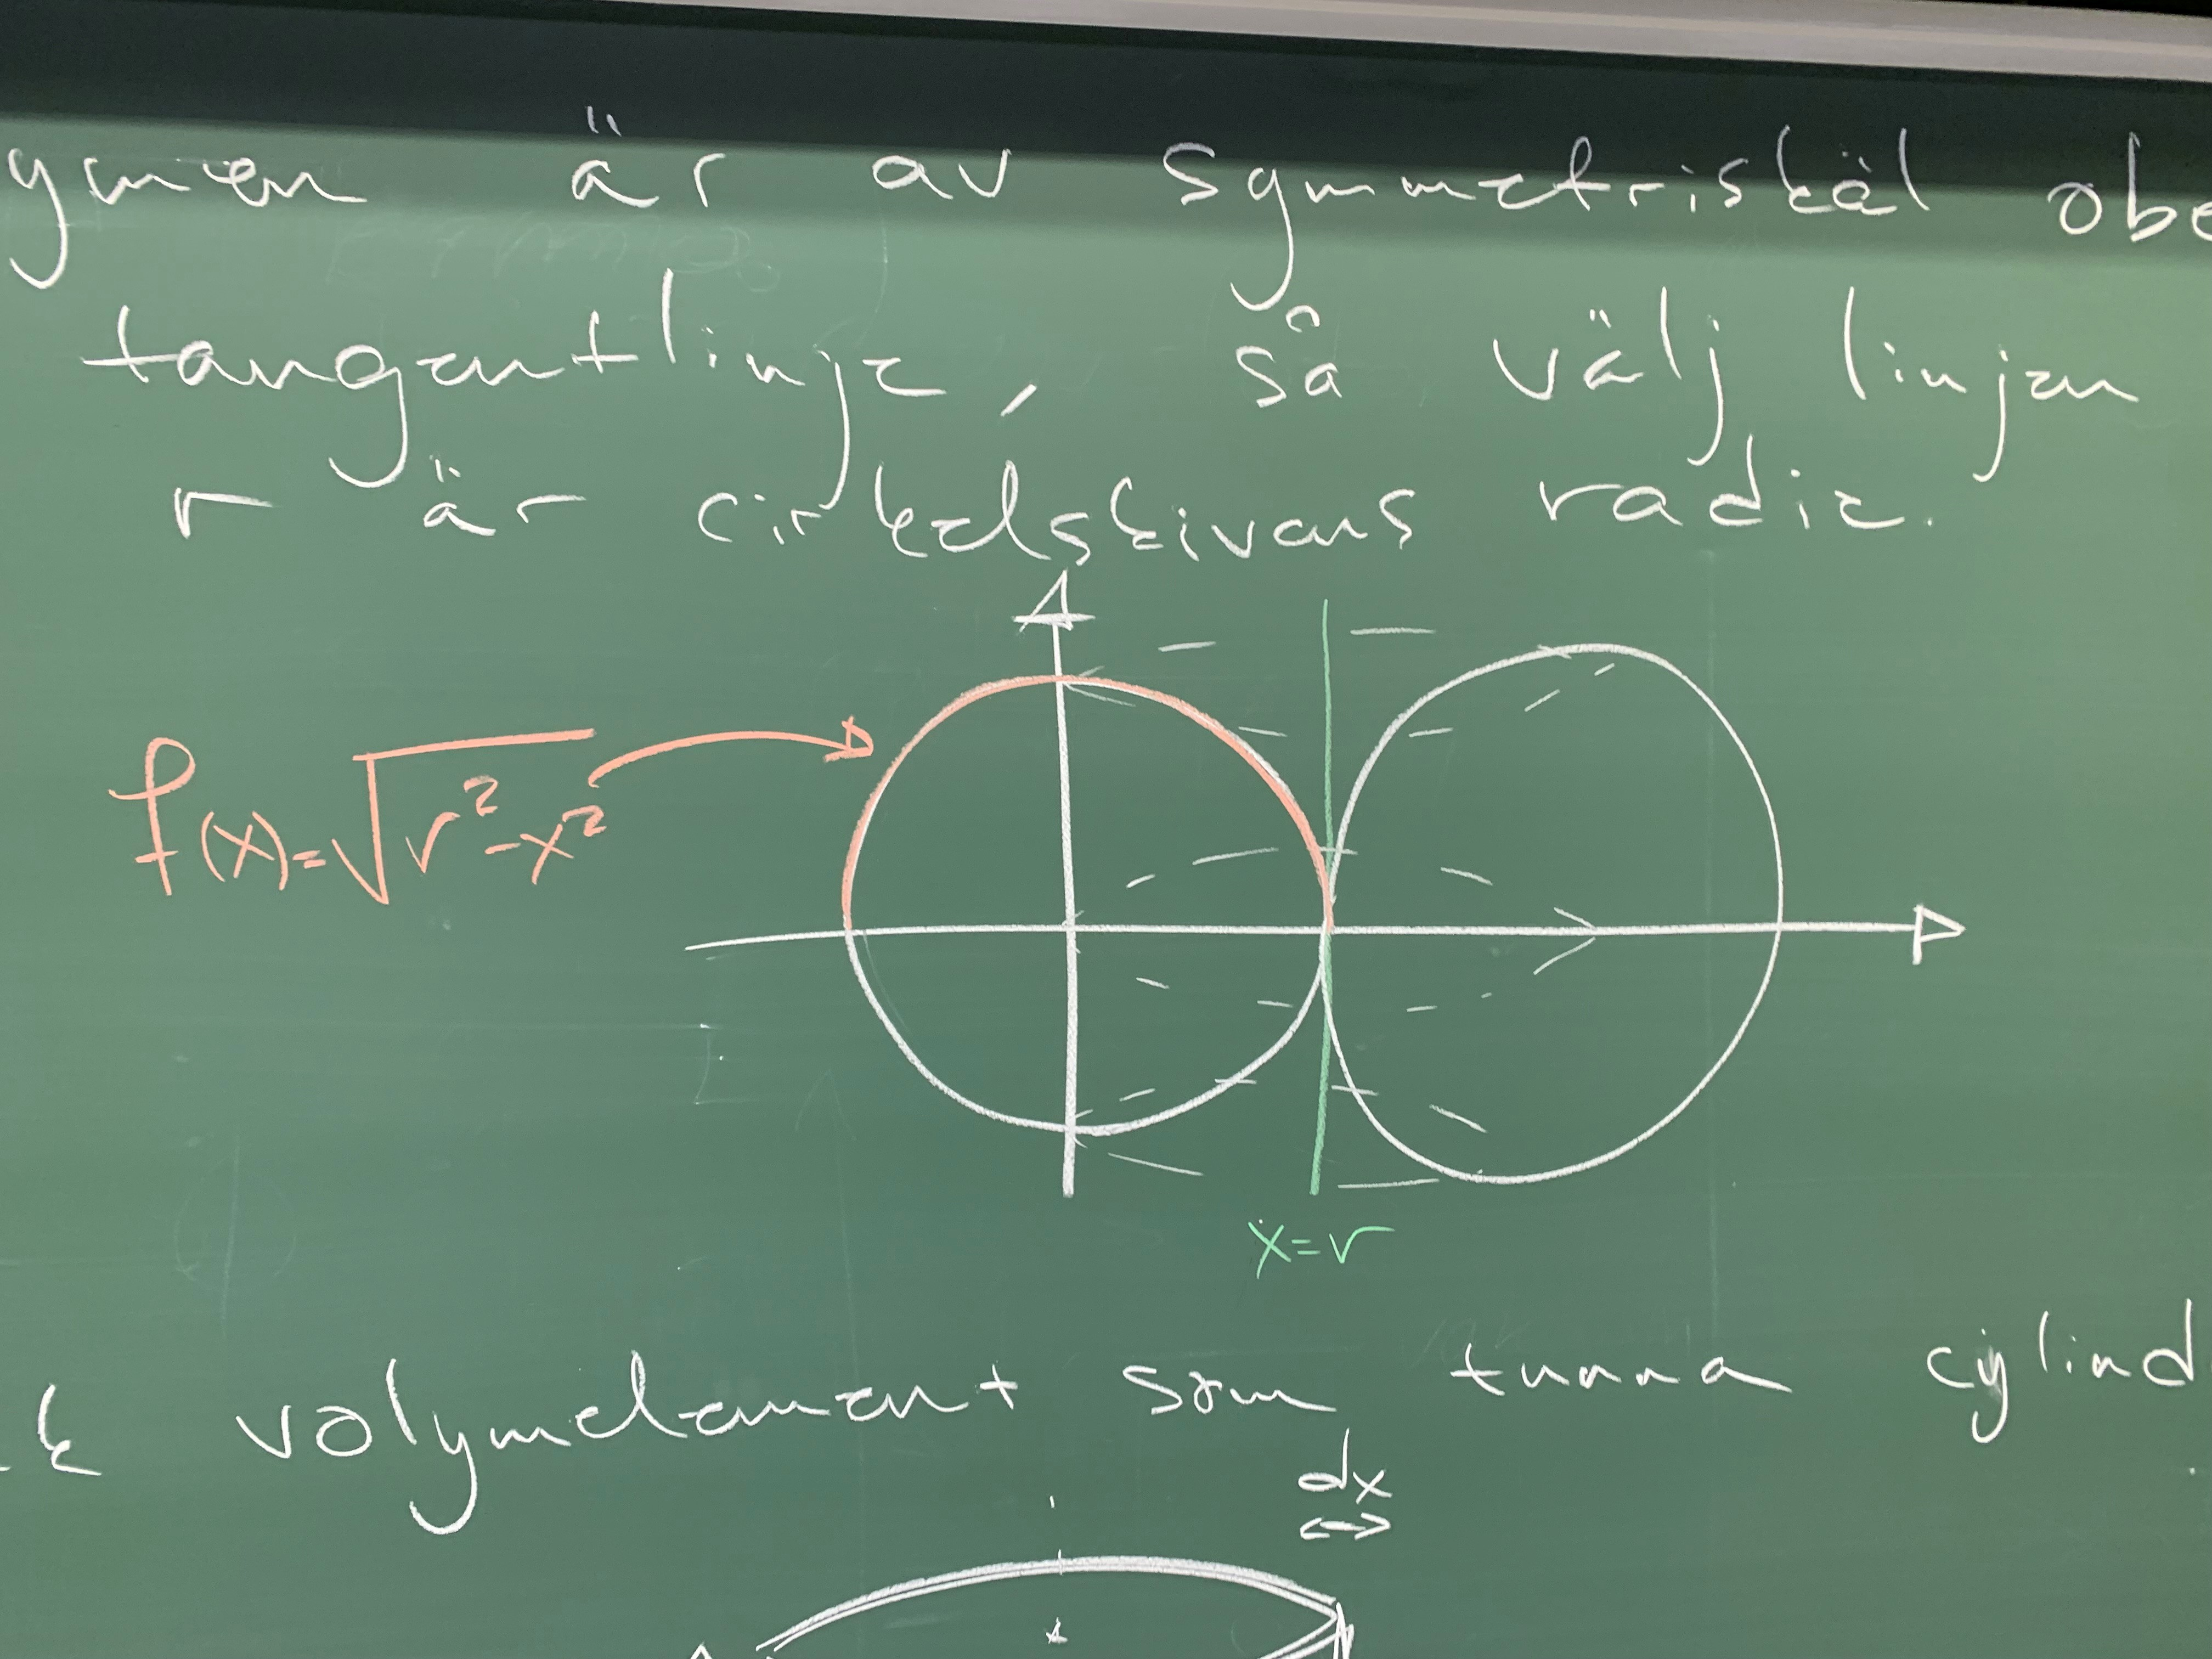
\includegraphics[scale=0.1]{lessons/lesson19/imgs/img07.jpg}
Tänk volym element som tunna cylindrar:
%infoga bild 8
%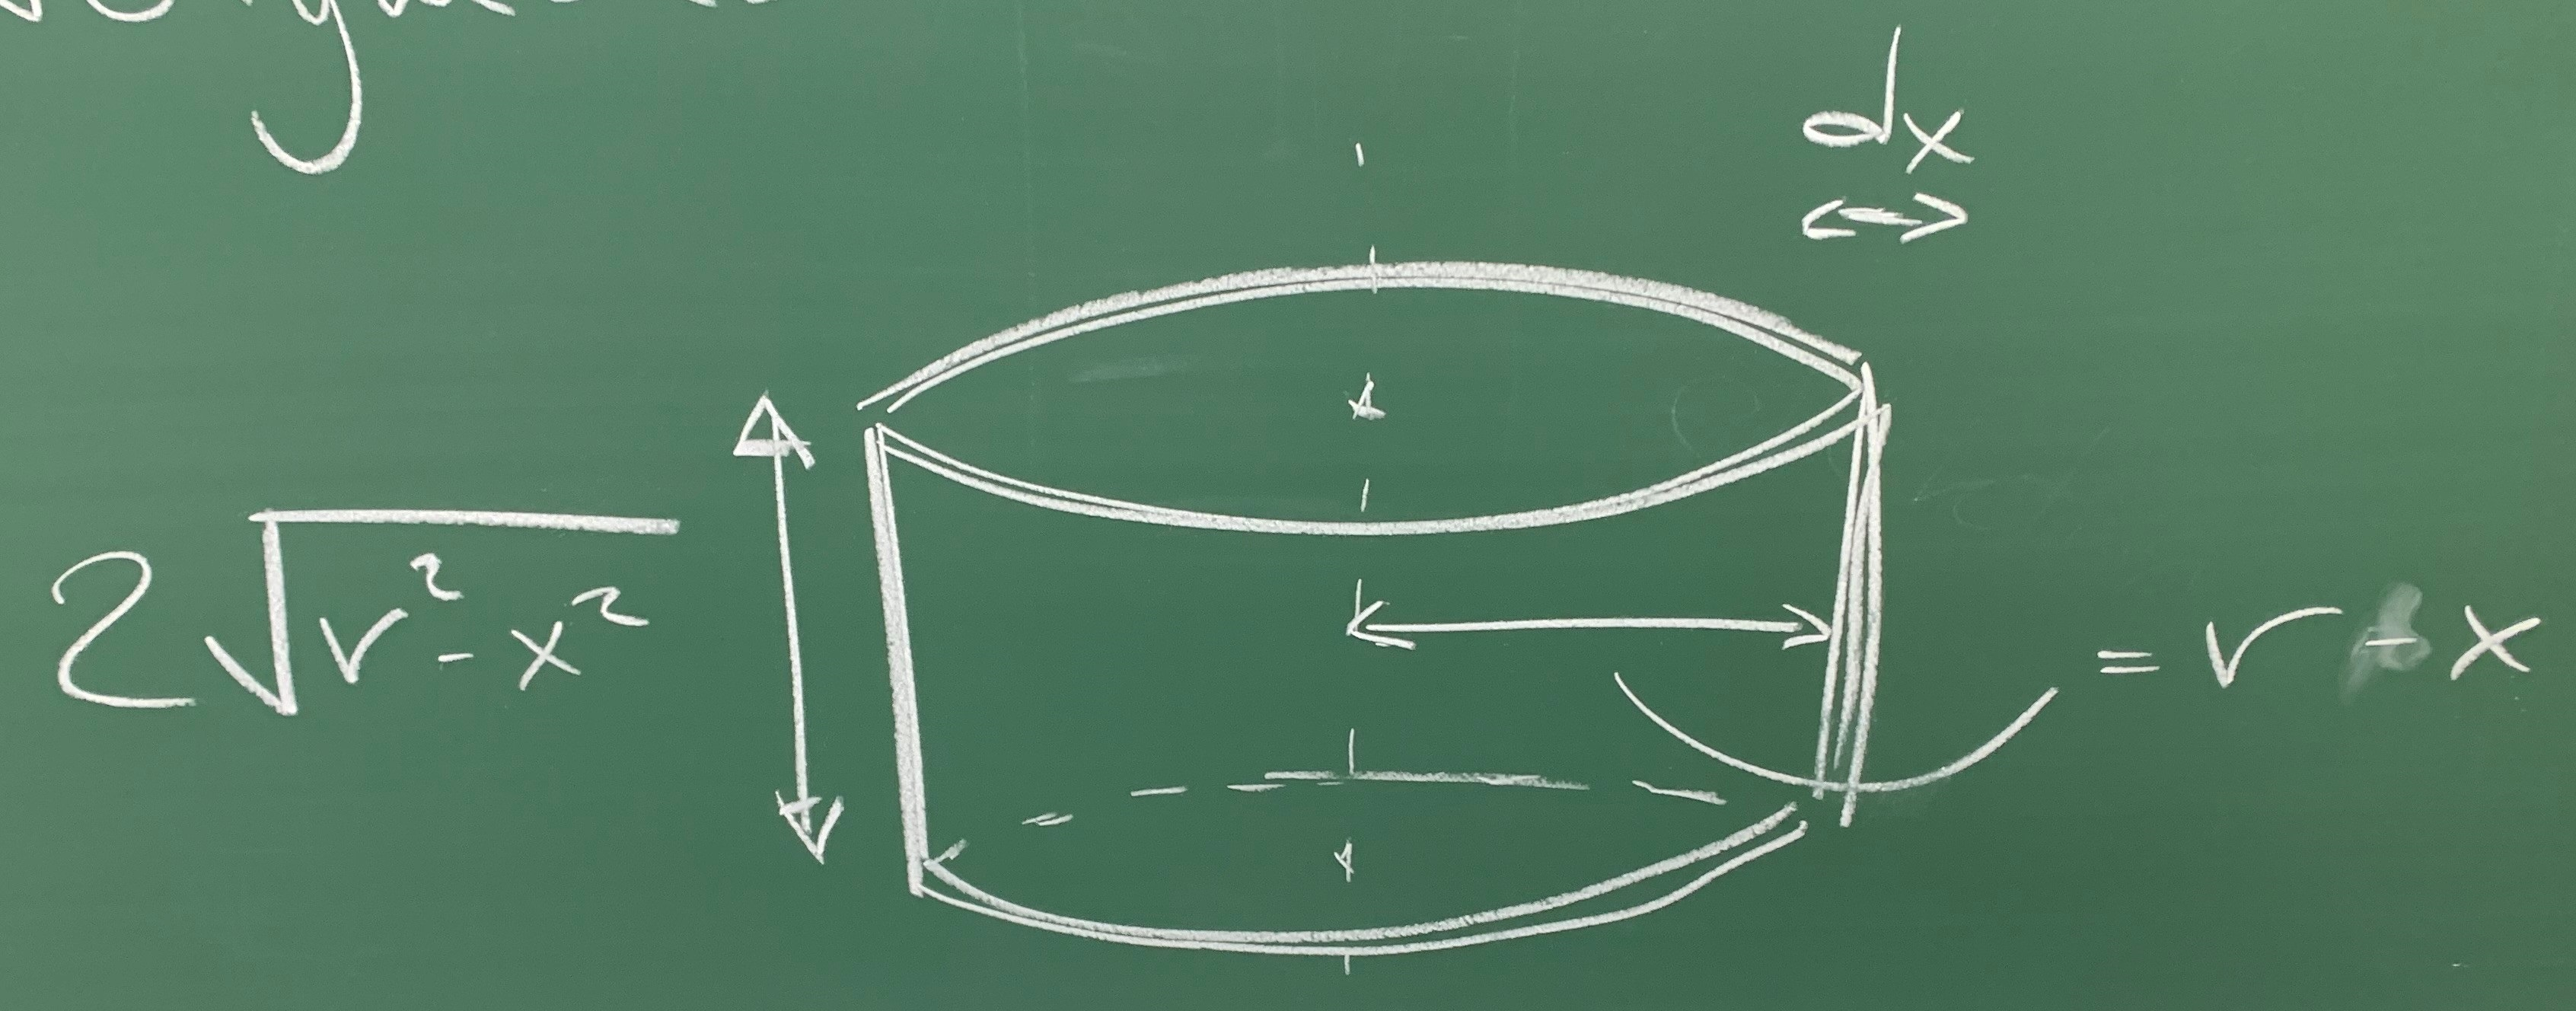
\includegraphics[scale=0.1]{lessons/lesson19/imgs/img08.jpg}
\begin{equation*}
    \rightarrow V=\int dV=\int_{-r}^r A(x)\, dx=
    \int_{-r}^r2\pi(r-x)\cdot 2\sqrt{r^2-x^2}\, dx=
\end{equation*}
\begin{equation*}
    4\pi[r\int_{-r}^r]\sqrt{r^2-x^2}\, dx - \int_{-r}^r x\sqrt{r^2-x^2}\, dx=
    4\pi r\int_{-r}^r\sqrt{r^-x^2}\, dx=
\end{equation*}
\begin{equation*}
    \{\text{arean av halvcirkeln}=\frac{\pi r^2}{2}\}=
    4\pi r\cdot\frac{\pi r^2}{2}=
    2\pi^2r^3 \Box
\end{equation*}

\section{Kurvlängd och mantelarea}
Kan approximera en kurva $C$ genom ett så kallat "polygontåg".\\
%infoga bild 9
%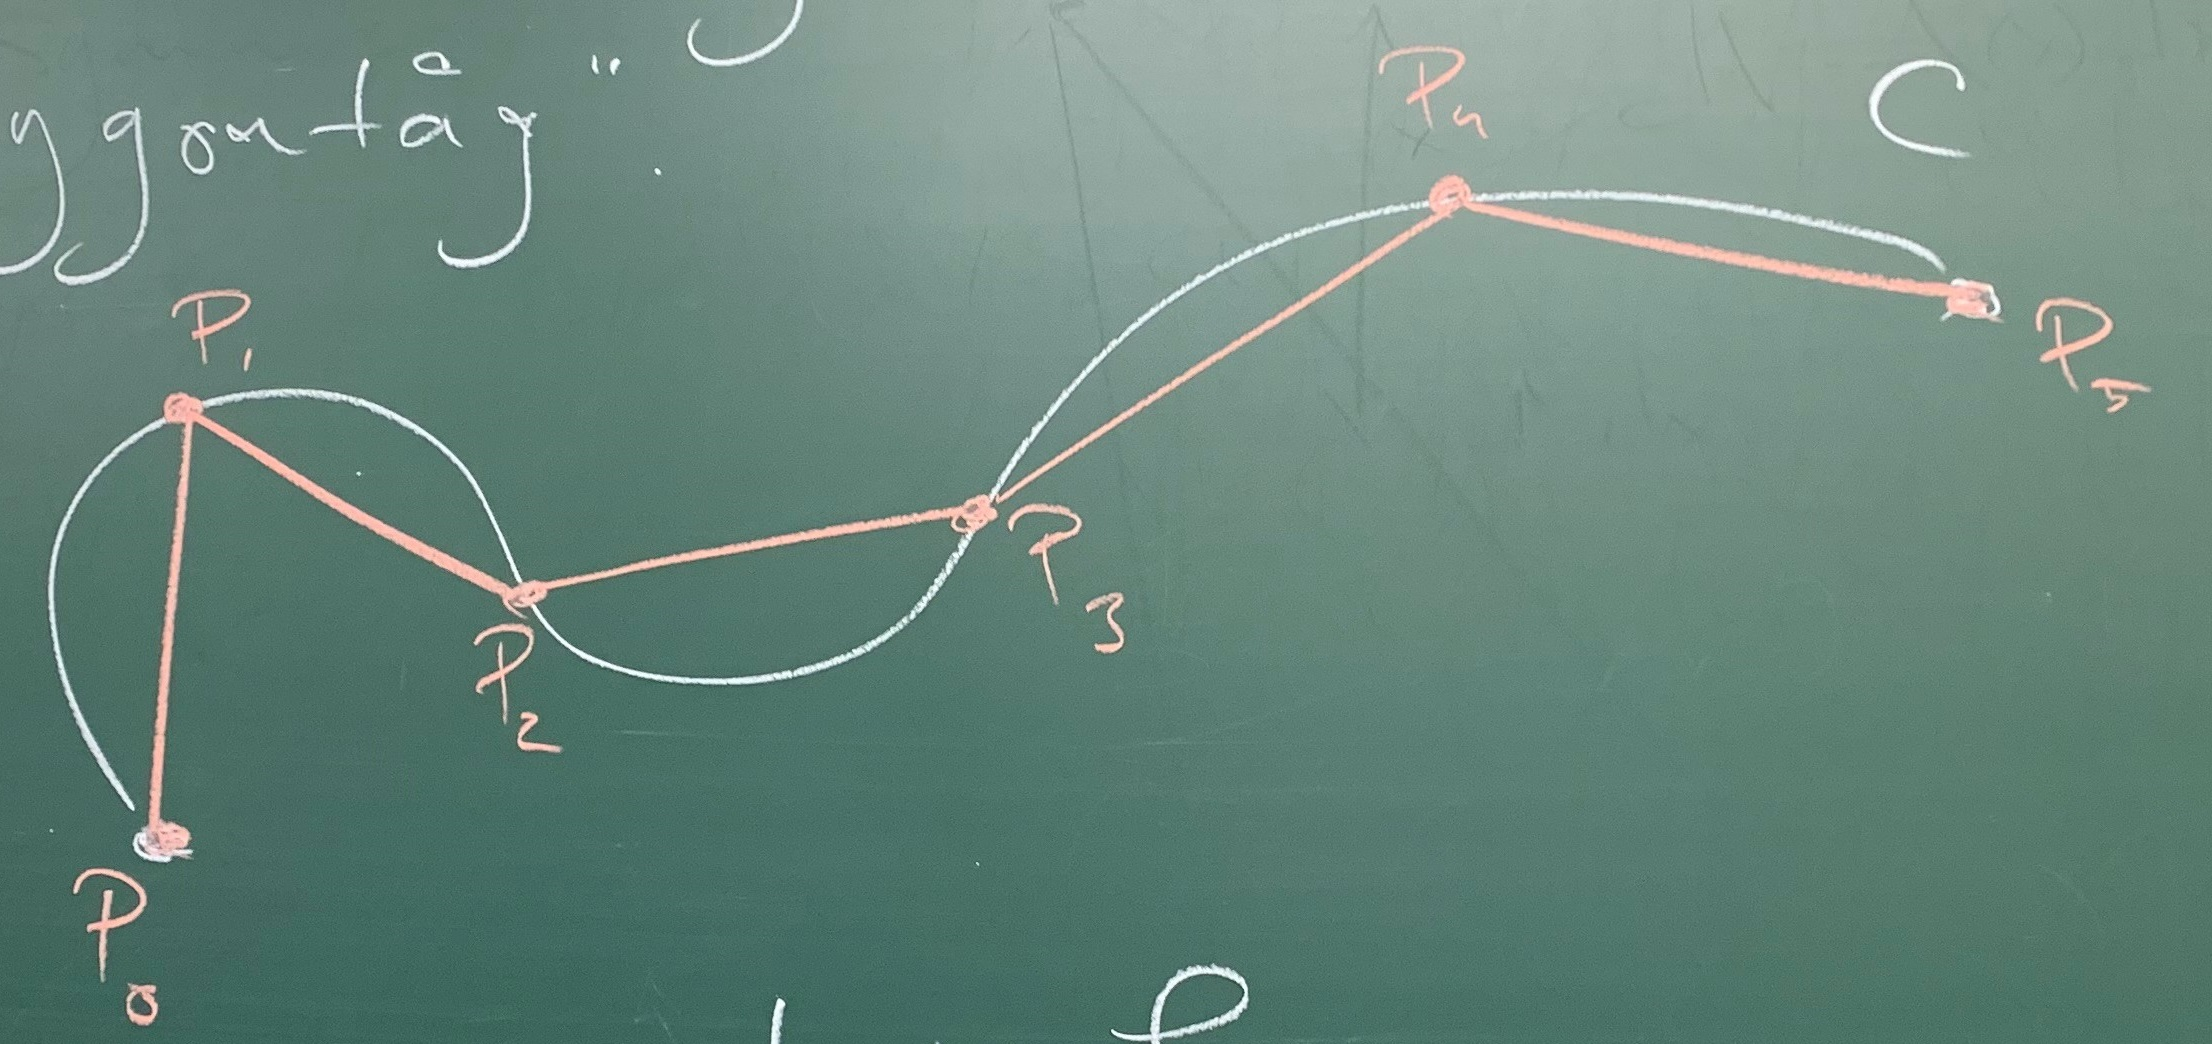
\includegraphics[scale=0.1]{lessons/lesson19/imgs/img09.jpg}
klart att det för varje polygontåg definierat av punkterna $\{P_0,P_1,...,P_n\}$ gäller att dess längd $L_n$ är kortare än den verkliga längden av $C$.
Man \underline{definierar} längden av $C$ som det minsta tal $s\in\mathbb{R}$ så att $L_n\leq s$ för alla polygontåg $\{P_0,P_1,...,P_n\}$.
Längden för ett linjesegment, säg mellan $P_i$ och $P_{i+1}$, blir:
%infoga bild 10
%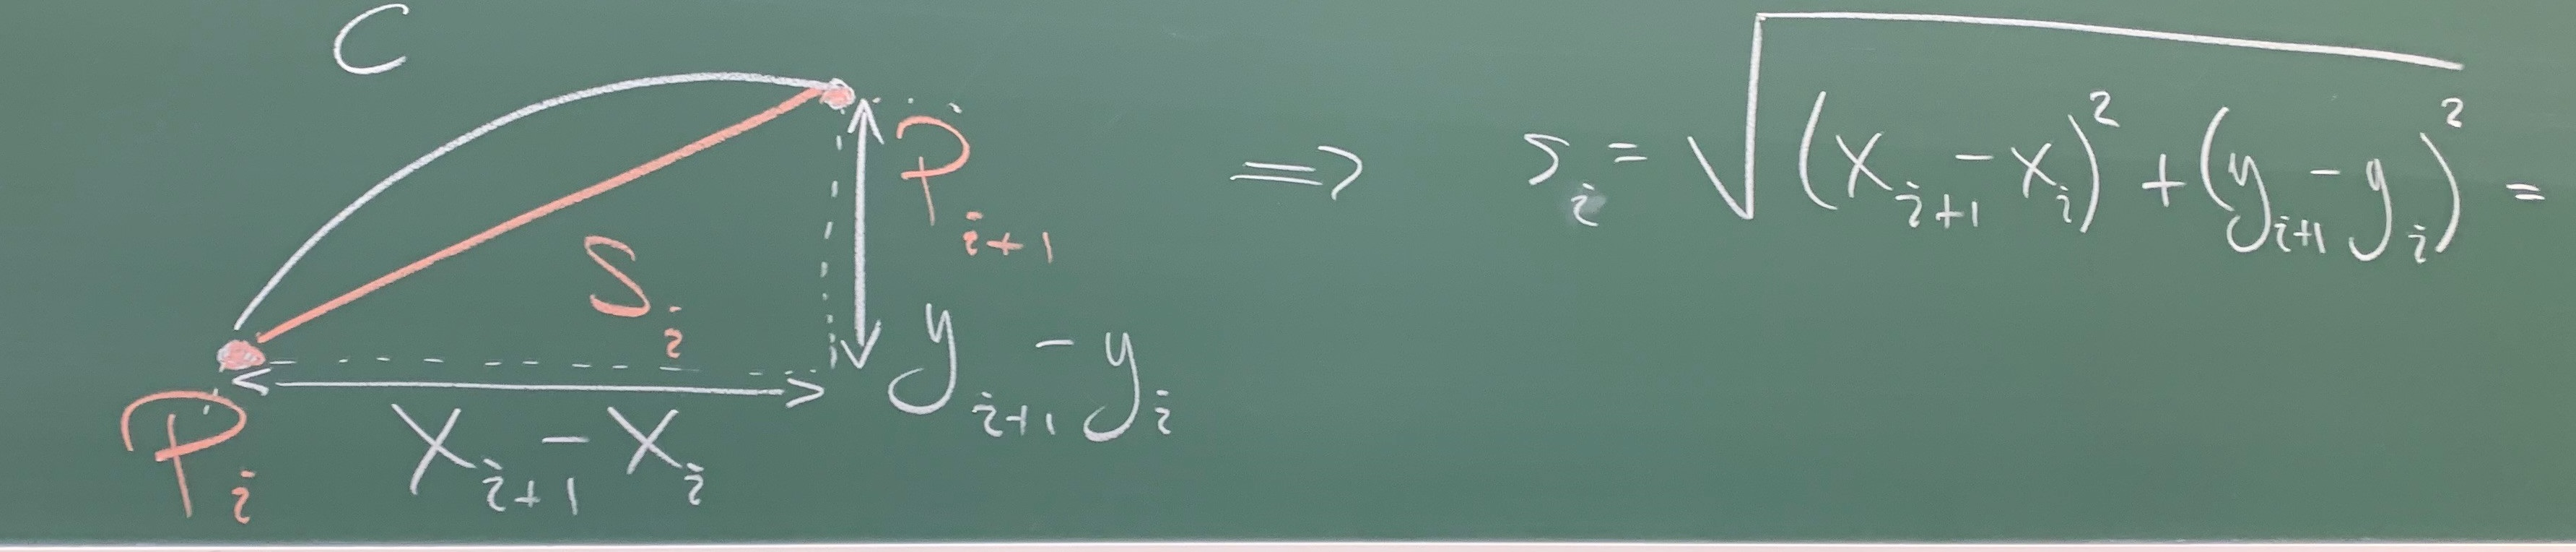
\includegraphics[scale=0.1]{lessons/lesson19/imgs/img10.jpg}
\begin{equation*}
    \Rightarrow s_i=
    \sqrt{(x_{i+1}-x_i)^2+(y_{i+1}-y_i)^2}=
    \sqrt{1+\frac{(y_{i+1}-y_i)^2}{(x_{i+1}-x_i)^2}}\cdot |x_{i+1}-x_i|
\end{equation*}
Om kurvans $y$-värden beskrivs av en funktion $f(x)$, polygontåget blir tätare och tätare och $f^\prime(x)$ existerar
\begin{equation*}
    s_i\to ds=\sqrt{1+(f^\prime(x))^2}\, dx
\end{equation*}
och $s=\int ds=\int_a^b\sqrt{1+(f^\prime(x))^2}\, dx$.

\paragraph*{Ex (7.3.12)} Bestäm längden av kurvan $x=-\frac{1}{2}$ och $x=\frac{1}{2}$ som definieras av grafen till $y=\ln(1-x^2)$.
\subparagraph{Lösning}
Kurvan kan skissas som\\
%infoga bild 11
%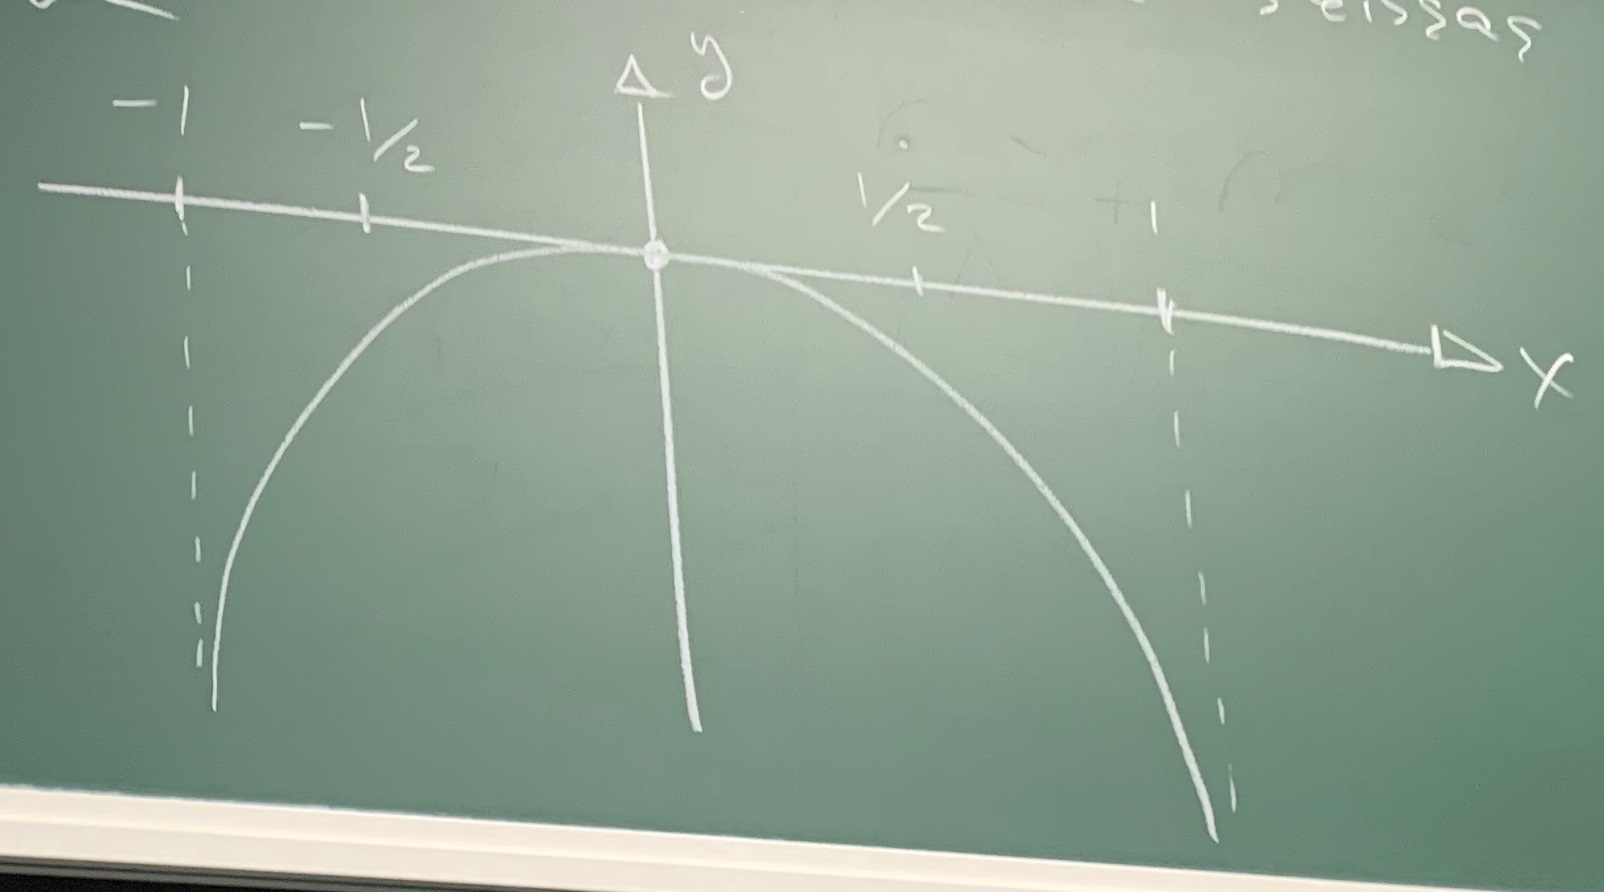
\includegraphics[scale=0.1]{lessons/lesson19/imgs/img11.jpg}
Det gäller att $y^\prime=\frac{1}{1-x^2}\cdot(-2x)=-\frac{2x}{1-x^2}$ för allla $x\in(-\frac{1}{2},\frac{1}{2})$ och alltså kan kurvans längd beräknas som:
\begin{equation*}
    s=\int_{-\frac{1}{2}}^\frac{1}{2}\sqrt{1+(-\frac{2x}{1-x^2})^2}\, dx=
    \int_{-\frac{1}{2}}^\frac{1}{2}\sqrt{1+\frac{4x^2}{(1-x^2)^2}}\, dx=
\end{equation*}
\begin{equation*}
    2\cdot\int_0^\frac{1}{2}\sqrt{1+\frac{4x^2}{(1-x^2)^2}}\, dx=
    2\int_0^\frac{1}{2}\sqrt{\frac{(1-x^2)^2+4x^2}{(1-x^2)^2}}\, dx=
\end{equation*}
\begin{equation*}
    2\int_0^\frac{1}{2}\sqrt{\frac{1-2x^2+x^4+4x^2}{(1-x^2)^2}}\, dx=
    2\int_0^\frac{1}{2}\sqrt{\frac{x^4-2x^2+1}{(1-x^2)^2}}\, dx=
\end{equation*}
\begin{equation*}
    2\int_0^\frac{1}{2}\sqrt{\frac{(x^2+1)^2}{(1-x^2)^2}}\, dx=
    2\int_0^\frac{1}{2}\frac{x^2+1}{1-x^2}=
    2\int_0^\frac{1}{2}\frac{x^2+1+2-2}{1-x^2}=
\end{equation*}
\begin{equation*}
    2\int_0^\frac{1}{2}\frac{2}{1-x^2}-1\, dx=
    \{\frac{2}{1-x^2}=\frac{A}{1+x}+\frac{B}{1-x}\Rightarrow A=B=1\}=
\end{equation*}
\begin{equation*}
    2\int_0^\frac{1}{2}\frac{1}{1+x}+\frac{1}{1-x}-1\, dx=
    2[\ln(|1+x|)-\ln(|1-x|)-x]_0^\frac{1}{2}=
\end{equation*}
\begin{equation*}
    2\cdot(\ln(\frac{3}{2})-\ln(\frac{1}{2})-\frac{1}{2})=
    2\ln(3)-1 \Box
\end{equation*}
Kan använda liknande teknik som för kurvlängder för att beräkna mantelytan av rotationssymmetriska kroppar till exempel om rotationssymmetrin längs $x$-axeln:\\
%infoga bild 12
%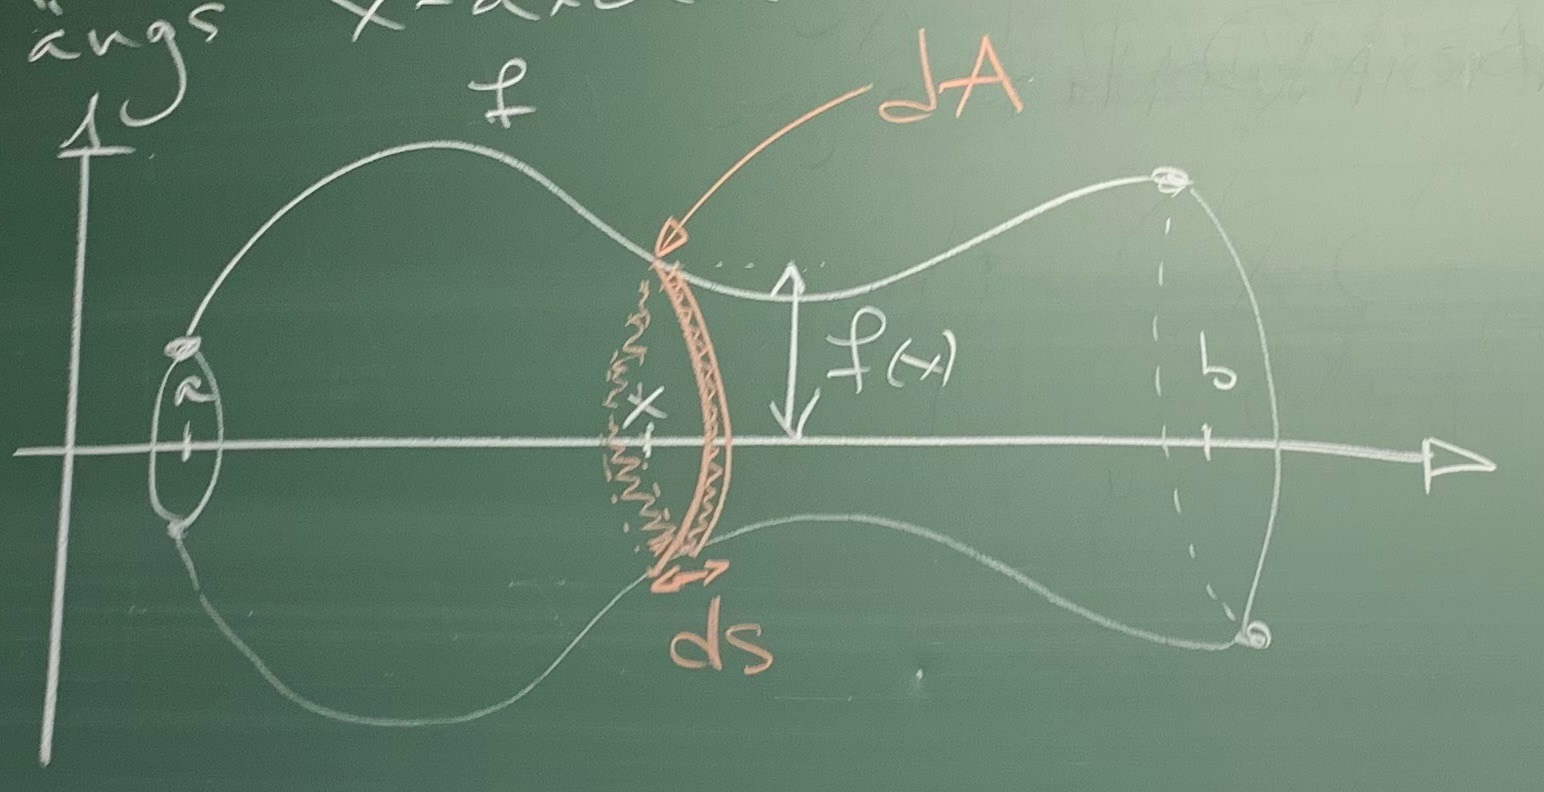
\includegraphics[scale=0.1]{lessons/lesson19/imgs/img12.jpg}\\
Måste hitta uttryck för area elementet $dA$ så att den totala mantelarean $A$ kan beräknas som $A=\int dA$.
Bandet med arean $dA$ kan "klippas upp" och tänkas som en rektangel med höjd $ds$ och längd $2\pi f(x)$, så:
\begin{equation*}
    dA=2\pi|f(x)|\, ds=
    2\pi|f(x)|\sqrt{1+(f^\prime(x))^2}\, dx
\end{equation*}
och allstå kan $A$ beräknas som
\begin{equation*}
    A=\int dA=2\pi\int_a^b|f(x)|\cdot\sqrt{1+(f^\prime(x))^2}\, dx
\end{equation*}
\section{Praktiska tillämpningar}
Inom klassisk mekanik studeras så kallade "stela kroppar", dvs. objekt som kan tänkas fullständigt oelastiska där inbördes relativa asvtånd är oförändrade under påverkan av yttre krafter.
För dessa r \underline{tyngdpunkt} ett centralt och viktigt begrepp.
För partikelsystem:\\
% infoga bild 1
% 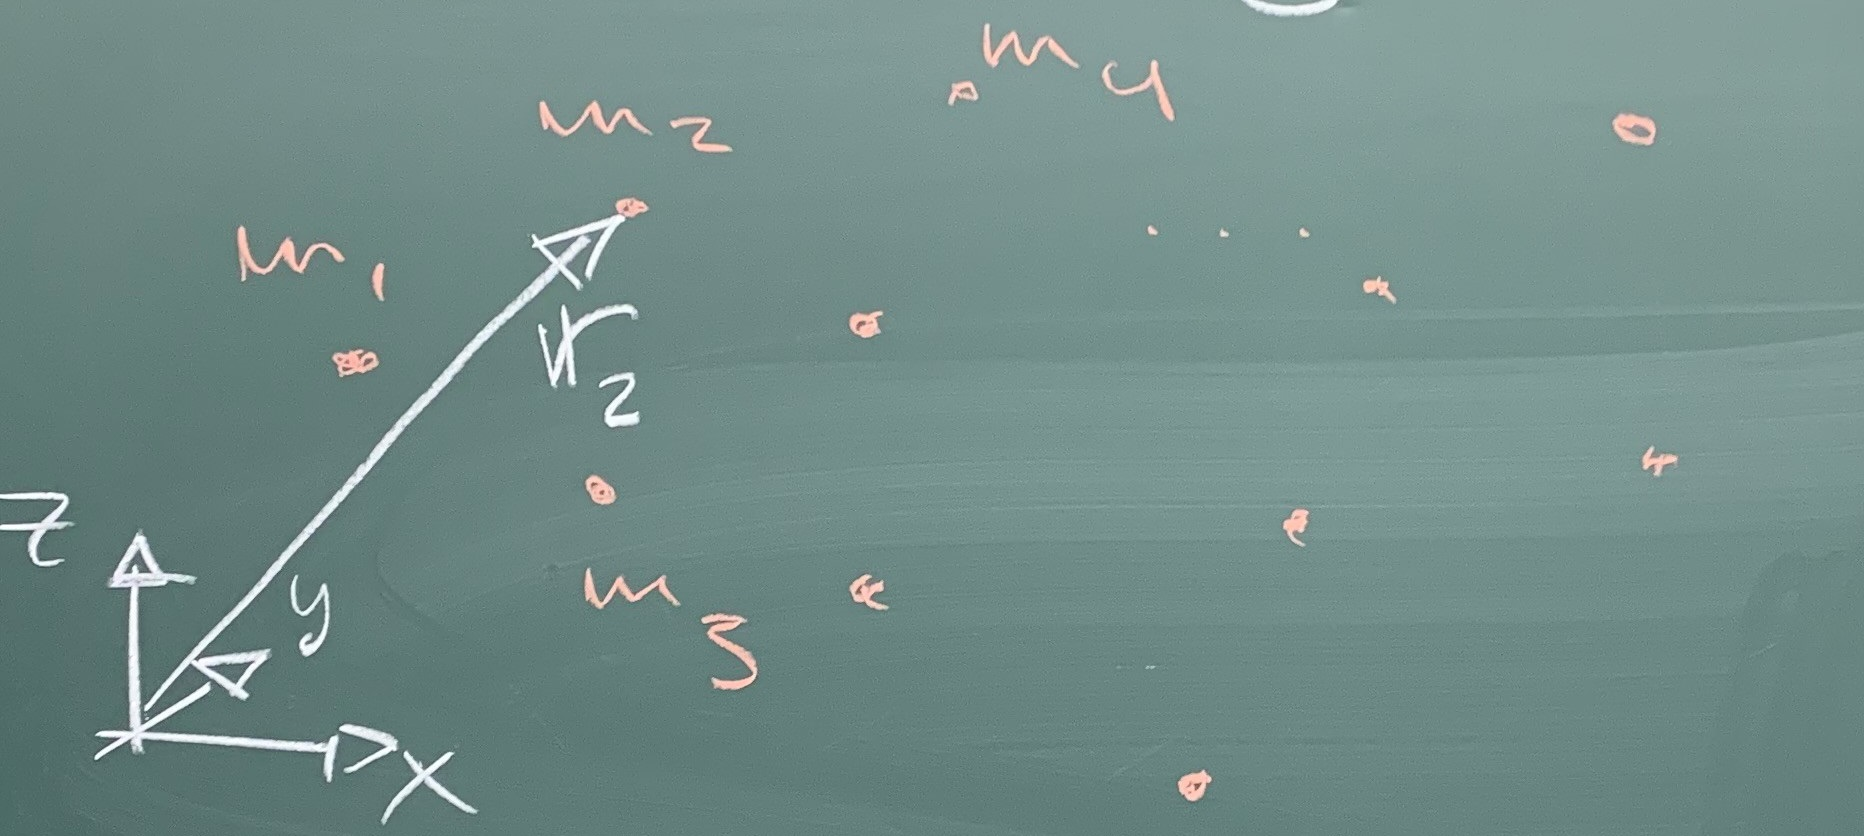
\includegraphics[scale=0.1]{lessons/lesson20/imgs/img01.jpg}\\
Systemets tyngdpunkt $\overline{r}$ definieras som:
\begin{equation*}
    \overline{r}=\frac{\sum_i r_i\cdot m_i}{\sum_i m_i}
\end{equation*}
Systemets moment betecknas $M_0$ och består av tre dimensionskomponenter:
\begin{equation*}
    M_0=(M_{x=0},M_{y=0},M_{z=0})
\end{equation*}
Vad blir motsvarande för en stel kropp vars densitet i en punkt $(x,y,z)$ beskrivs av $\varrho (x,y,z)$.
Stel kropp:\\
%infoga bild 2
%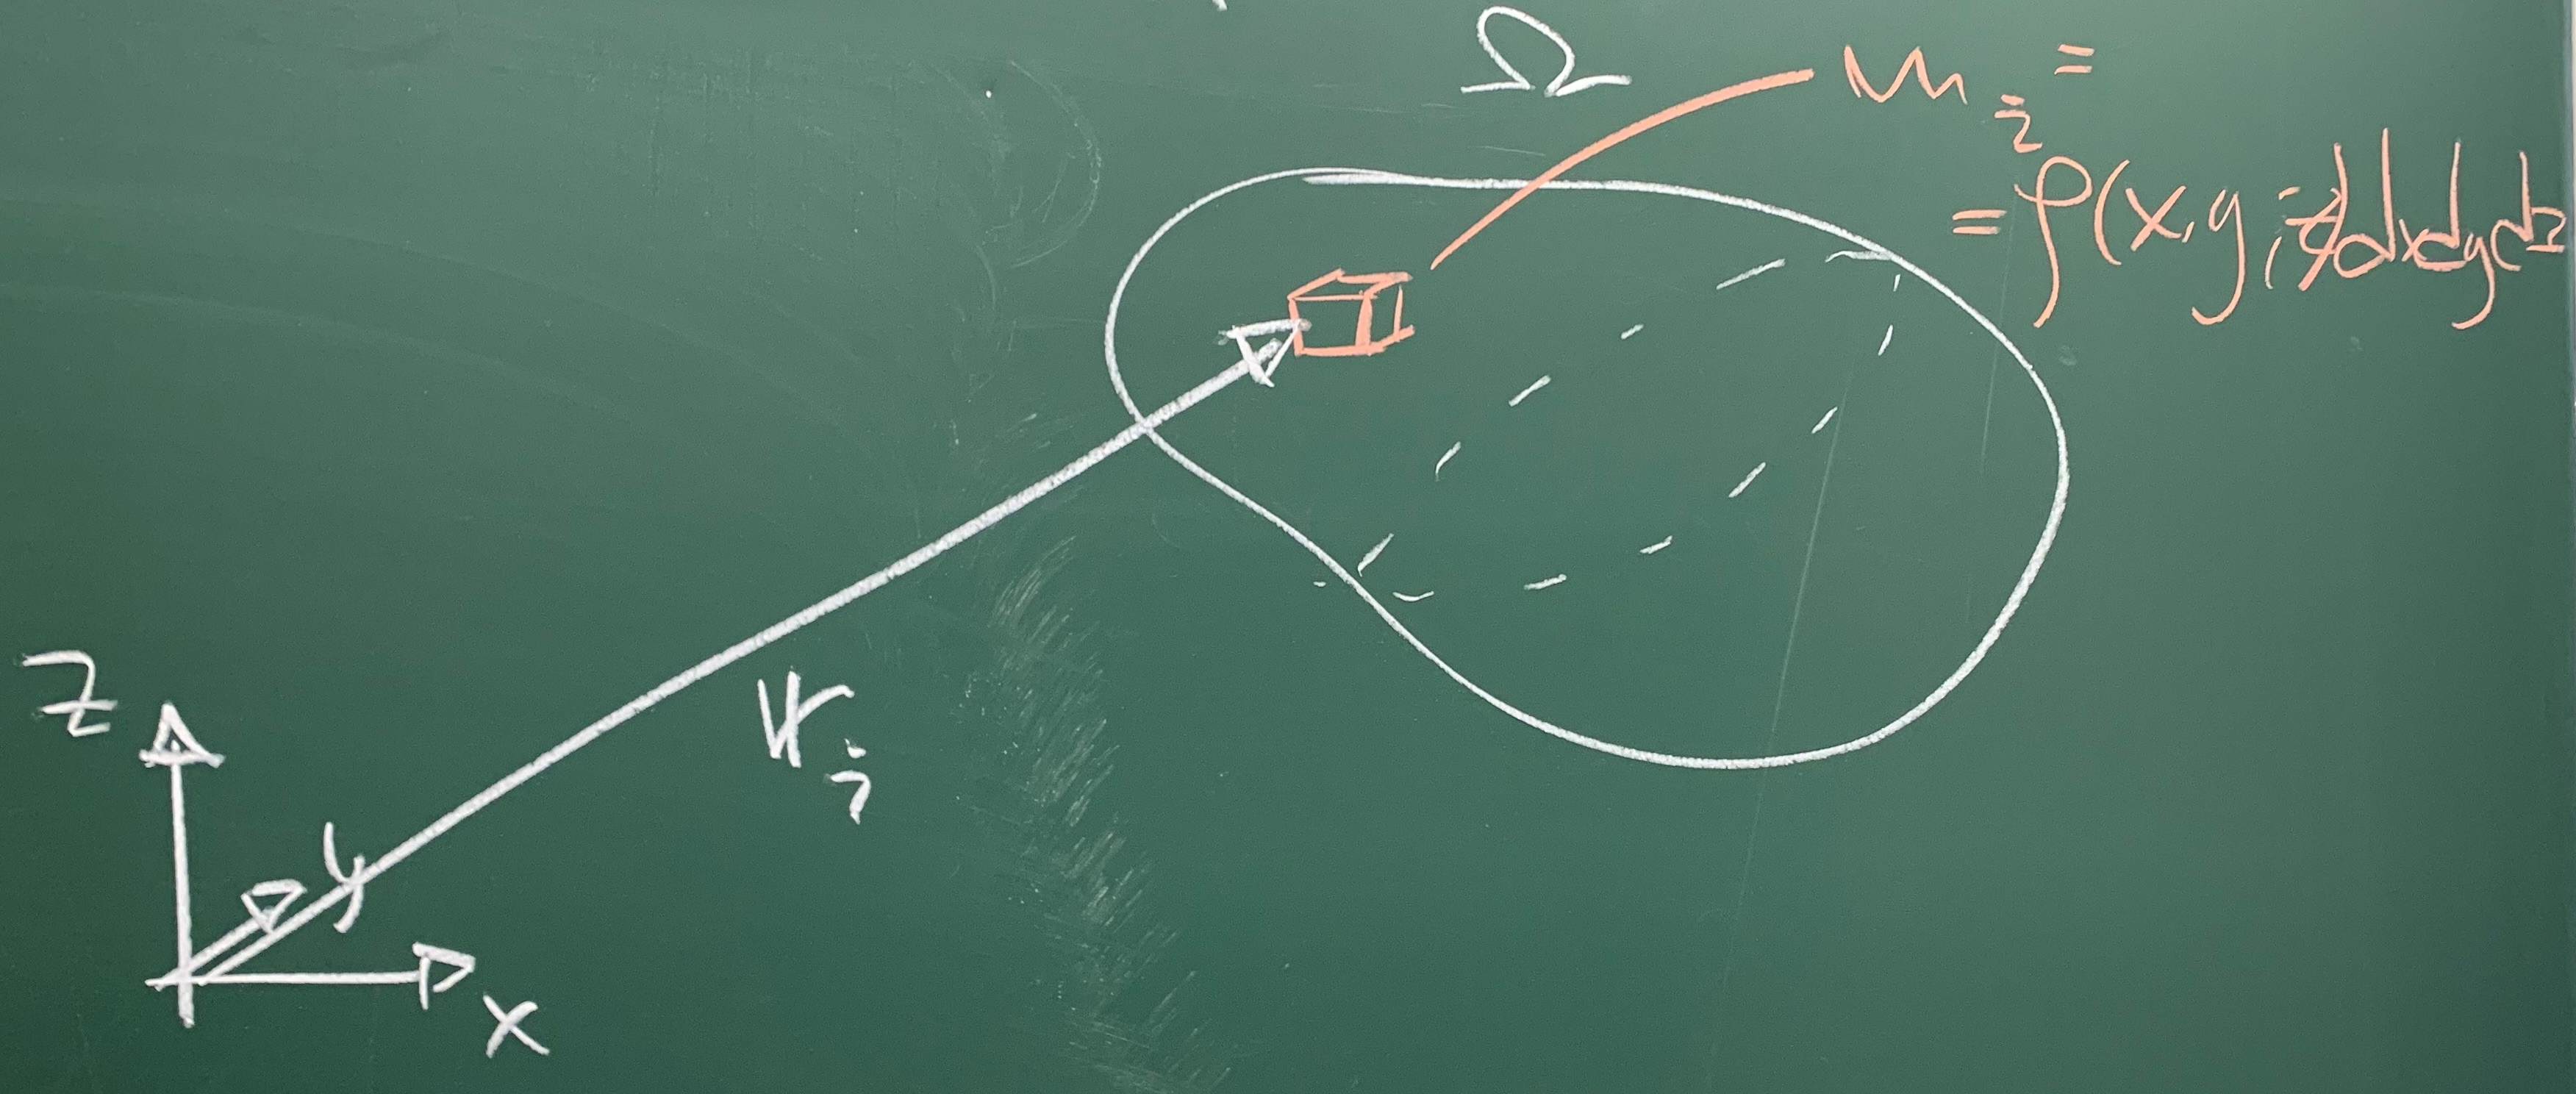
\includegraphics[]{lessons/lesson20/imgs/img02.jpg}\\
så tyngdpunkten för den stela kroppen blir:
\begin{equation*}
    \overline{r}=
    \sum_i \frac{m_i \overline{r}_i}{\sum_i m_i}\to
    \frac{\int_\Omega (x,y,z)\cdot\varrho(x,y,z)\, dx\, dy\, dz}{\int \varrho(x,y,z)\, dx\, dy\, dz}
\end{equation*}
Om man kan identifiera symmetrier ibland $\overline{r}$ beräknas med hjälp av "enkelintegraler".

\paragraph{Ex (7.4.7)} Beräkna tyngdpunkten för en kvadratisk platta med sidan $a$ cm om dess areadensitet är $\varrho(x)=k\cdot x$ g/cm$^2$ där $x$ är asvtåndet mellan en punkt $P$ på plattan och en av plattans sidor.
\subparagraph{Lösning}
Lägg plattan i ett koordinatsystem där "referenssidan" för plattans densitet är sammanfaller med y-axeln.\\
%infoga bild 3
%\includegraphics[scale=0.1]{lessons/lesson20/imgs/img03.jpg}\\
Uppenbart av symmetriskäl att tyngdpunkten i $y$-led ligger på höjden $\frac{a}{2}$.
Plattans totala massa $m$ blir:
\begin{equation*}
    m=\int dm=\int_0^a kx\cdot a\cdot\, dx=ka[\frac{x^2}{2}]_0^a=\frac{ka^3}{2}
\end{equation*}
Och momentet runt $x=0$ betecknas $M_{x=0}$, blir:
\begin{equation*}
    M_{x=0}=\int x\, dm=\int_0^a x\cdot kx\cdot a\cdot\, dx=ka[\frac{x^3}{3}]_0^a=\frac{ka^4}{4}
\end{equation*}
så tyngdpunkten i $x$-led hamnar i $\overline{x}=\frac{M_{x=0}}{m}=\frac{\frac{ka^3}{3}}{ka^3/2}=\frac{2a}{3}$
dvs. $\overline{r}=(\frac{2a}{3},\frac{a}{2}) \Box$

\paragraph*{Ex (7.4.14)} Beräkna tyngdpunkten för en boll med radie $R$ (m) om bollens densitet i en punkt $P$ är $\varrho(z)=z$ kg/m$^3$ där $z$ är asvtånd från $P$ till ett plan $2R$ m från bollems mittpunkt.
\subparagraph{Lösning}
% infoga bild 4
%\includegraphics[scale=0.1]{lessons/lesson20/imgs/img04.jpg}\\
Med angivet koordinatsystem angivet enligt bild så är det givet att bollens tyngdpunkt i $x$- respektive $y$-led är $0$ på grund av symmetri och att densiteten endast varierar i $z$-led, dvs. $\overline{r}=(0,0,\overbrace{z})$.
Använd plattor parallella med  $xy$-planet för att beräkna $m$ och $M_{z=0}$.\\
% infoga bild 5
%\includegraphics[scale=0.1]{lessons/lesson20/imgs/img05.jpg}
\begin{equation*}
    \Rightarrow dm=
    (2R-z)\cdot\pi(\sqrt{R^2-z^2})^2\, dz=
    \pi(2R-z)(R^2-z^2)\, dz
\end{equation*}
\begin{equation*}
    \Rightarrow m=
    \int dm=
    \int_{-R}^R\pi(2R-z)(R^2-z^2)\, dz=
    \pi\int_{-R}^R 2R^3-2Rz^2-zR^2+z^3\, dz=
\end{equation*}
\begin{equation*}
    \pi[2R^3z-\frac{2}{3}Rz^3]_{-R}^R=
    \frac{8}{3}\pi R^4
\end{equation*}
\begin{equation*}
    M_{z=0}=\int_{-R}^R z\, dm=
    \int_{-R}^R z\cdot\pi(2R-z)(R^2-z^2)\, dz=
    ...=
    \frac{4\pi}{15}R^5\Rightarrow
\end{equation*}
\begin{equation*}
    \overline{z}=\frac{4\pi\frac{R^5}{15}}{\frac{8\pi R^4}{3}}=
    ...=
    \frac{R}{10}\Box
\end{equation*}

\paragraph*{Ex (7.6.3)} En damm är $200$ m lång, $24$ m hög och är utformad som en $26$ m lång slip.
Om Vattenytan står vid dammens topp, hur stor kraft måste den då hålla emot från vattentrycket?
\subparagraph{Lösning}
%infoga bild 6
%\includegraphics[scale=0.1]{lessons/lesson20/imgs/img06.jpg}\\
Det hydrostatiska trycket på djupet $h$ m ges av $p=\varrho\cdot g\cdot h$ där $\varrho$ är vattnets densitet och $g$ är tyngdaccelerationen.\\
Betrakta en tunn delyta på dammen som kan betraktas som utsatt för ett konstant tryck.
Om ytans area är $dA$ så utsätts denna för en kraft $dF=p\cdot dA=\varrho g h\, dA$.
Vad är $dA$?\\
% infoga bild 7
%\includegraphics[scale=0.1]{lessons/lesson20/imgs/img07.jpg}
$dA=200\cdot ds=200\frac{dh}{\sin(\alpha)}$ där $\sin(\alpha)=\frac{24}{26}$ ($\Rightarrow\alpha\approx 67.4^\circ$) så
\begin{equation*}
    F_{\text{tot}}=
    \int dF=
    \int_0^24\varrho g h \cdot 200 \cdot\frac{dh}{\sin(\alpha)}=
    200\varrho g\frac{26}{24}\int_0^24h\, dh=
    200\varrho g\frac{26}{24}[\frac{h^2}{2}]_0^24=
    6.12\cdot10^8 \text{ N}
\end{equation*}

\paragraph{Ex (7.6.9)} Beräkkna det arbete som krävs för att pumpa allt vatten ur en (sfärisk) skål med radie $a$ m till en höjd $h$ m ovanför skålens top.
\subparagraph{Lösning}
%infoga bild 8
%\includegraphics[]{lessons/lesson20/imgs/img08.jpg}
Beräkna det arbete som krävs för att lyfta en tunn cirkulär vattenskiva från skålen till höjden $h$ enligt bild.
För cirkelbågen gäller att
%infoga bild 9
\begin{equation*}
    \text{så }dm=
    \varrho dV=
    \varrho A(x)\, dx=
    \varrho\pi f^2(x)\, dx=
    \varrho\pi(a^2-x^2)\, dx
\end{equation*}
Arbete att lyfta en massa $m$ till höjden $h$  ges av $W=mgh$ och alltså
\begin{equation*}
    dW=
    \varrho g\pi(a^2-x^2)(x+h)\, dx=
    \varrho g\pi(a^2x+a^2h-x^3-xh^2)\, dx
\end{equation*}
För att lyfta skvian vid $x$ till höjden $h$ krävs det totala arbetet $W_{\text{tot}}$ enligt
\begin{equation*}
    W_{\text{tot}}=
    \int dW=
    \int_0^a\varrho g\pi(a^2x+a^2h-x^4-hx^2)\, dx=
\end{equation*}
\begin{equation*}
    \varrho g\pi[\frac{a^2}{2}x^2+a^2hx-\frac{x^4}{4}-\frac{h}{3}x^3]_0^a=
    \varrho g\pi(\frac{a^4}{2}+a^3h-\frac{a^4}{4}-\frac{a^3h}{3})=
    \varrho g\pi(\frac{a^4}{4}+\frac{2a^3h}{3})=
\end{equation*}
\begin{equation*}
    \frac{\varrho g\pi a^3}{4}(a+\frac{8h}{3})=
    2450\pi a^3(a+\frac{8h}{3})\text{ J}\Box
\end{equation*}

% Exercises
%\chapter{Övningar}
%Här är kommer uppgifter med lösningar från övningspassen
%\section*{P1}
\paragraph{21}~\\
Lös olikheten $x^2-2x\leq 0$. Svara i termer av intervall.\\
\underline{Notera:} $f(x)=x^2-2x$ är kontinuerlig på hela reella linjen.
\paragraph{Lösning:}~\\
Först löser vi nollställen till vänsterledet, alltså $x^2-2x$.
Vi ställer upp följande:
\begin{equation*}
    x^2-2x=0\Leftrightarrow x(x-2)=0
\end{equation*}
Då är våra lösningar $x=0$ och $x=2$.
Med denna information gör vi en tabell.
\begin{equation*}
    \begin{matrix}
                   &   & 0 &   & 2 &   \\
        x          & - & 0 & + & + & + \\
        x-2        & - & - & - & 0 & + \\
        \text{Tot} & + & 0 & - & 0 & +
    \end{matrix}
\end{equation*}
Då $x$ ska vara mindre än $0$ letar vi efter intervallet i tabellen som uppfyller det kravet.
I denna uppgiften var det $[0,2]$
\underline{Svar:} $[0,2]$
\section*{P2}
\paragraph{29}~\\
Finn intercept och lutning till linjen $\sqrt{2}x-\sqrt{3}y=2$. Skissa grafen till linjen.
\paragraph{Lösning}~\\
Linjen korsar x och y axeln då y respektive x är 0.
Alltså:
\begin{itemize}
    \item $x=0$ ger: $0-\sqrt{3}y=2\Leftrightarrow y=-\frac{2}{\sqrt{3}}$
    \item $y=0$ ger: $\sqrt{2}x-0=2\Leftrightarrow x=\frac{2}{\sqrt{2}}=\sqrt{2}$
\end{itemize}
Nu har vi två punkter där linjen korsar x- och y-axeln, $(0, -\frac{2}{\sqrt{3}})$ och $(\sqrt{2}, 0)$.
Med $\frac{\Delta y}{\Delta   x}$ kan vi räkna ut lutningen.
\begin{equation*}
    \frac{-(-\frac{2}{\sqrt{3}})+0}{0-\sqrt{2}}=
    \frac{\frac{2}{\sqrt{3}}}{\sqrt{2}}=
    \frac{\sqrt{2}}{\sqrt{3}}
\end{equation*}
\underline{Svar:} $\frac{\sqrt{2}}{\sqrt{3}}$

\paragraph{33}~\\
Finn skärningspunkterna till linjerna $3x+4y=-6$ och $2x-3y=13$.
\paragraph{Lösning:}~\\
Vi ställer upp de båda linjerna i ett ekvationssystem.
Man kan lösa detta genom gausselimination men vi gör det genom substitution.
\begin{equation*}
    \begin{matrix}
        3x+4y=-6 \\
        2x-3y=13
    \end{matrix}
\end{equation*}
Vi separerar $x$:
$3x+4y=-6\Leftrightarrow 3x=-6-4y\Leftrightarrow x=-2-\frac{4}{3}y$\\
Vi substituerar $x$ med det vi fick:
\begin{equation*}
    2x-3y=13\Leftrightarrow
    2\cdot(2-\frac{4}{3}y)-3y=13\Leftrightarrow
    -4-\frac{8}{3}y-\frac{9}{3}=13\Leftrightarrow
    -\frac{17}{3}y=17\Leftrightarrow
    -\frac{1}{3}y=1\Leftrightarrow y=-3
\end{equation*}
Då vi vet vad $y$ är kan vi räkna ut punktens x värde med ytterliggare en substitution.
$4x+4(-3)=-6\Leftrightarrow 3x=6\Leftrightarrow x=2$\\
\underline{Svar:} $(2, -3)$

\section*{A1}
\paragraph{13}~\\
Bestäm absolutbeloppet och argument för $z=\sqrt{3}-i$

\paragraph{Lösning}~\\
Absolutbeloppet av ett komplext tal räknas ut genom att betrakta talet
som en punkt i det komplexa talplanet och räkna ut avståndet från origo
till punkten.\\
Alltså använder vi pythagoras sats:
$|z|^2=(\sqrt{3})^2+1^2=3+1=4\Leftrightarrow |z|=\sqrt{4}=2$.\\
Nu ska vi räkna ut $arg(z)$.
Vi får en triangel som har sidorna $\sqrt{3},1,2$.
Vinkeln kan man då räkna ut med $tan(\frac{1}{\sqrt{3}})=30^\circ$.
\underline{Svar:} $|z|=2$ och $arg(z)=30^{circ}$


\end{document}